\documentclass{book}

\usepackage{amsmath,amssymb}
\usepackage{amsfonts}
\usepackage{latexsym}
%\usepackage{psfig}
\usepackage{graphicx}
\usepackage{noweb}
\usepackage{caption}
\usepackage{color}\pagecolor{white}
\usepackage{algorithm}
\usepackage[noend]{algpseudocode}
%\usepackage{fontspec}
%\newfontfamily\devanagarifont{Noto Sans Devanagari}[Script=Devanagari]
\usepackage[utf8]{inputenc}
\usepackage{pgfplots}
 % or any recent installed version
\usepackage{tfrupee}
\pgfplotsset{compat=1.17}

\usepackage{hyperref}
\hypersetup{
    colorlinks,
    citecolor=blue,
    filecolor=black,
    linkcolor=blue,
    urlcolor=blue
}
\hypersetup{unicode=true}  % for Unicode in PDF bookmarks
\usepackage{microtype}
\usepackage{tikz} 
\usetikzlibrary{rulercompass,arrows.meta,positioning,fit,calc,patterns}
\usetikzlibrary{arrows.meta} % for nice arrowheads (optional)
\tikzset{>=Stealth}

\newtheorem {theorem}{Theorem}[chapter]
\newtheorem {claim}{Claim}[chapter]
\newtheorem{eqed}{Example}[chapter]
\newtheorem {lemma}{Lemma}[chapter]
\newtheorem {observation}[theorem]{Observation}
\newtheorem {remark}{Remark}[chapter]
\newtheorem {defn}{Definition}[chapter]
\newtheorem{definition}{Definition}[chapter]   % or [section]
\newtheorem {corl}{Corollary}[chapter]
\newtheorem {corollary}[theorem]{Corollary}
\newtheorem {proposition}[theorem]{Proposition}
\newtheorem {fact}[theorem]{Fact}
\newtheorem {example}{Example}[chapter]
\newtheorem {exercise}{Exercise}[chapter]
\newenvironment{proof}{{\it Proof:\ } }{\hfill$\Box$ }
\def\dmodels{\stackrel{\tenmi D}\models}
\def\implies{\Longrightarrow}
\def\leqv{\Longleftrightarrow}
\def\logeqv{\Longleftrightarrow}
\def\N{\mathbb{N}}
\def\Z{\mathbb{Z}}
\def\R{\mathbb{R}}
\def\Q{\mathbb{Q}}
\def\B{\mathbb{B}}
\def\P{\mathbb{P}}
\def\D{\mathbb{D}}
\def\eq{\Leftrightarrow}
\def\down{\downarrow}
\def\lamda{{\bf \lambda}}
\def\alphL{\alpha\!\!-\!\!LIST}
\newcommand{\Scheme}{{\tt Scheme }}
\newcommand{\Pascal}{{\tt Pascal }}
\newcommand{\C}{{\tt C }}
\newcommand{\Fortran}{{\tt Fortran }}
\newcommand{\ML}{{\tt ML }}
\newcommand{\Java}{{\tt Java }}
\newcommand{\Py}{{\tt Python }}
\newcommand{\Python}{{\tt Python }}

\setlength{\textheight}{9.0in}
\setlength{\textwidth}{6.0in}
\setlength{\topmargin}{-.25in}
\setlength{\headheight}{0.5in}
\setlength{\headsep}{0.25in}
\setlength{\evensidemargin}{0.0in}
\setlength{\parindent}{1pc}


\begin{document}

\title{\Large\bf Lecture Notes: Quantitative Reasoning and Mathematical Thinking\footnote{
Copyright \copyright~~  2025, Subhashis Banerjee.
 All Rights Reserved. These notes may be used in an academic
course with prior consent of the author.}
}

\author{Subhashis Banerjee\\[2mm]
{\em	Department of Computer Science } \\
{\em	Ashoka University} \\
{\em	Sonipat, Haryana, 131029 }\\
{\em	email: suban@ashoka.edu.in} \\
\\
}

\date{\today}

\maketitle
\tableofcontents
\chapter{Introduction}
\label{chap:intro}


Courant and Robbins, in \href{https://en.wikipedia.org/wiki/What_Is_Mathematics\%3F}{What is Mathematics? (1941)}, present mathematics not as a dry collection of formulas and tools, but as a living, creative discipline rooted in human thought and curiosity. For them, mathematics is both a pathway for understanding the natural world and an autonomous intellectual pursuit that reveals structures of order, beauty, and generality. They stress that its essence lies in the interplay between abstraction and concrete problem-solving: starting from simple, practical problems, mathematics ascends to general concepts and theories that then illuminate new domains.

They emphasize accessibility and unity: mathematics belongs to everyone who is willing to think rigorously, and its spirit combines logic with imagination. Rather than reducing it to calculation or technical skill, Courant and Robbins describe mathematics as “an expression of the human mind” where precision, creativity, and aesthetic appreciation converge. Their central idea is that mathematics is at once useful, philosophical, and artistic — simultaneously a language of science, a training ground for reasoning, and a source of intellectual delight.

Early mathematics was computational when the emphasis was on finding methods to obtain solutions. However, over the years, the disciplines of mathematics and computer science -- the subject of designing algorithms for problem solving -- have diverged. In mathematics abstraction is symbolic and logical. It seeks general structures, patterns, and proofs independent of implementation. It often endeavours to seek and  capture  common structures across different abstractions. The primary aim is truth and understanding -- developing rigorous proofs, ensuring logical consistency, and uncovering general laws. Utility often follows from this pursuit but is not always the main driver. In contrast, the role of abstraction in computational thinking  is more operational and algorithmic. It emphasizes creating computational process models for natural, social and even abstract phenomena for operational analysis. The primary aim is to construct effective procedures -- designing algorithms that solve problems efficiently, often under constraints of time, memory, and real-world complexity. The power lies in execution and exploration — trying to  reveal insights about systems too complex to solve analytically.  Both have become fundamental strands of epistemology that are essential for critical scientific thinking.

Data-driven inference represents a third way of knowing, distinct from the deductive rigour of mathematics and the constructive procedures of computational thinking. As practiced in modern data science and machine learning, it seeks knowledge not by proving theorems or designing explicit algorithms, but by discovering patterns and regularities directly from empirical data. Its epistemic core is induction at scale: hypotheses, models, or predictors are justified by their ability to capture hidden correlations and to generalize to new observations. Unlike mathematics, correctness is not absolute, and unlike computational thinking, procedures are not always fully transparent. Instead, credibility arises from empirical adequacy — the degree to which models explain, predict, or align with observed phenomena. This mode of inference expands our epistemic toolkit for a world where complexity and abundance of data overwhelm deductive or constructive methods, but it also brings new philosophical challenges: uncertainty about correctness, bias, and the gap between correlation and causation.

In this course we will try to cover some fundamentals of all of the above.


\chapter{God gave us numbers, and human thought created algorithms}
\label{chap:sets_and_numbers}

\begin{figure}[ht]
\begin{center}
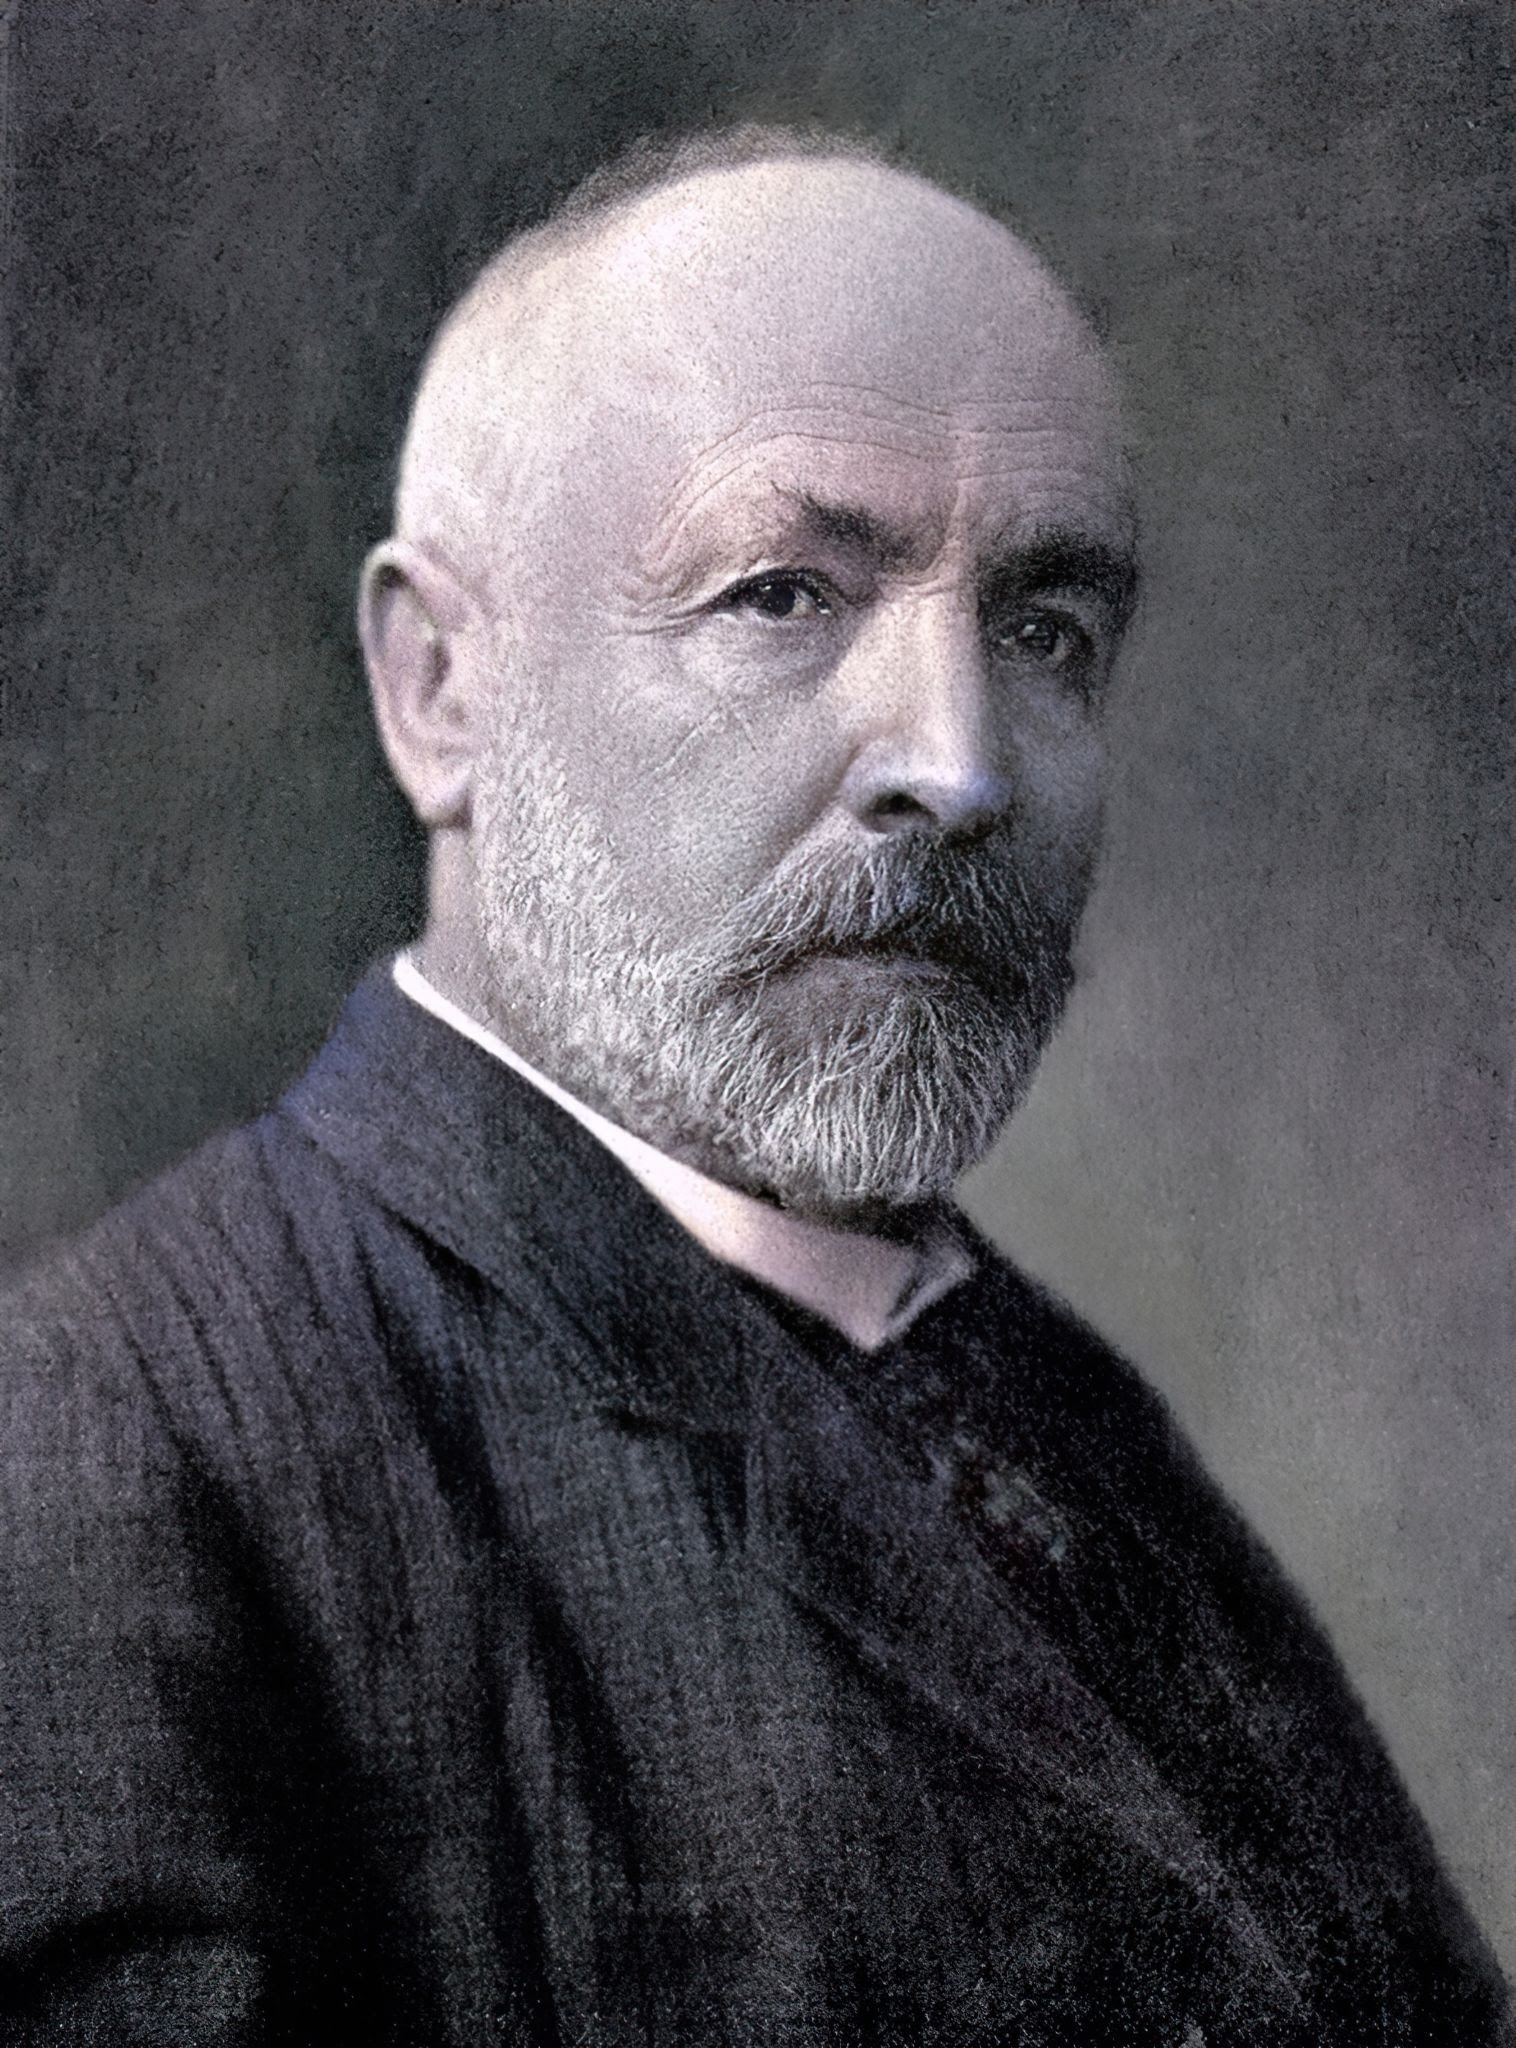
\includegraphics[width=1.0in]{images/cantor.jpeg}

\caption*{\small ``In mathematics the art of proposing a question must be held of higher value than solving it.'' \\
``A set is a Many that allows itself to be thought of as a One.''   -- Georg Cantor}
\end{center}
\end{figure}


\begin{figure}[ht]
\begin{center}
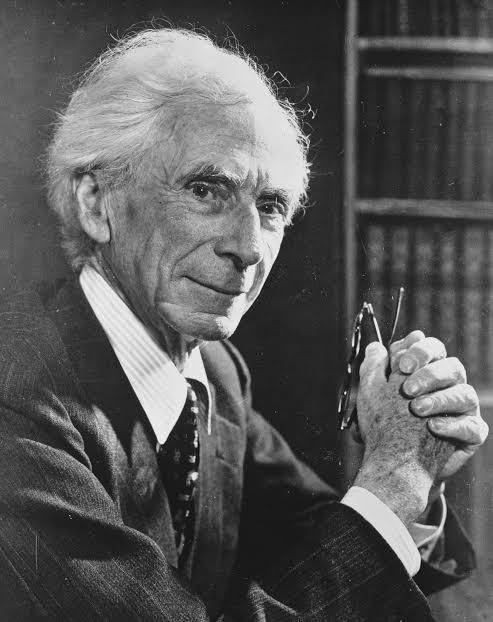
\includegraphics[width=1.0in]{images/russell.jpeg}
\caption*{\small ``A number will be a set of classes such as that any two are similar to each other,  and none outside the set are similar to any inside the set.'' \\
                ``Mathematics rightly viewed possesses not only truth but supreme beauty.'' -- Bertrand Russel}
\end{center}
\end{figure}

\section{Numbers}
\label{sec:numbers}
Our discussion on mathematics and computing must start with numbers. What are numbers after all? The same number may be represented  with symbols such as 3,  III, or even as a line of a fixed length. But what is the underlying concept behind the different representations?

\href{https://en.wikipedia.org/wiki/Bertrand_Russell}{Bertrand Russell} defined numbers as sizes (or {\em cardinality}) of {\em collections}. Some examples of  {\em equinumerous} collections are $\{Red, Blue, Green\}$, $\{Amir, Salman, Shahrukh\}$, $\{Godavari, Kaveri, Krishna\}$. {\em Collections} are also called {\em Sets} or {\em Classes} in Mathematics. All three Sets above are of cardinality 3. Russel defined a number as -- {\em the number of a class is the class of all those classes that are similar (equinumerous) to it}. So, according to Russel, a number is a class of classes.  

Note that {\em cardinality} of sets is not the only way to describe the concept of a number. A number may also be a measure of a length. For example, in the straight line below, if we define the segment $\overline{0a}$ to be the {\em unit length} representing the number 1, then the line segment $\overline{0b}$ which is twice the length of $\overline{0a}$ may  represent the number 2.

\vspace{0.5in}
\begin{tikzpicture}[stop jumping,constrain]
\path(0,0) node[name=O,ruler compass/point=red,label={0}];
\path (O)++(0:2) node[ruler compass/point=red,label={a}];
\ruler{O}{a}
\path (a)++(0:2) node[ruler compass/point=red,label={b}];
\ruler{a}{b}
%\compass{O}{a}
\end{tikzpicture}
\vspace{0.5in}

Without belabouring the point, it will suffice to say for our purpose that all of us intuitively understand what numbers mean.

\subsection{Numbers may be represented in multiple ways}

However, we need to do useful stuff with numbers -- we need to add, subtract, multiply and divide them for obvious practical reasons.  Indeed, the history of numbers date back to the Mesolithic stone age. The early humans had to figure out -- due to a variety of practical considerations -- that if they put two similar collections of size two and size three together, the larger collection becomes of size five.  

Civilisations have found many ways to represent numbers through the ages. Some examples are as tally marks in the prehistoric to early civilisations  -- as straight marks on bones, sticks, or stones --  as can be observed in the archaeological evidence of the Ishango bones from around 20000 BCE; as Egyptian --  a stroke for 1, heel bone for 10, coil of rope for 100, etc. -- or Roman -- I, V, X, L, C, D, M -- numerals; as Base-60 (sexagesimal) numbers written as combinations of ``1'' and ``10'' wedges by the Babylonians around 2000 BCE; as used rods arranged on counting boards in base-10 with positional notation in Chinese rod systems;  as positional decimal systems in Indian numerals in the Gupta period around $5^{th}$ century CE;  as beads or stones moved on rods or grooves to represent numbers in Abacus systems in China, Rome, Mesopotamia and Jerusalem; with  Indo-Arabic numerals in the medieval period; with various mechanical calculators such as  Napier’s bones,  Slide rules,  Pascal’s calculator, and  Leibniz's stepped reckoner in the $17^{th}$ century; as gears and levers in Charles Babbage's first programmable computer -- the Analytic Engine; and as bits and bytes in modern digital computers. Note, also, that the methods of carrying out these operations -- the algorithms -- will necessarily depend on the representation we choose for numbers. 

\section{Sets}
\label{sec:sets}
We will use {\em Sets} quite a bit in this course. We may describe a {\em Set} or a {\em Collection} by explicitly listing out its elements without duplicates, such as in the examples above. We may sometimes also describe a Set with a property like ``all students enrolled in the QRMT section FC-0306-3". We write this formally using a variable $x$ as $\{x \mid \mbox{$x$ is a student in the QRMT section FC-0306-3}\}$. The symbol $\mid$ is read as ``such that". 

If an element $x$ belongs to a set $A$, we usually write this as $x \in A$.

Here are some more examples of Sets:
\begin{enumerate}
\item $A = \{x \mid \mbox{$x$ is a student pursuing a degree in India}\}$
\item $B = \{x \mid  \mbox{$x$ is a CS Major student at Ashoka University}\}$
\item $C = \{x \mid \mbox{$x$ is a CS Major student at Ashoka University {\bf and} $x$ is female}\}$
\end{enumerate}

Clearly, all members of $C$ are also members of $B$, and all members of $B$ are members of $A$. We then say that $C$ is a {\em subset} of $B$  ($C \subseteq B$), and  $B$ is a {\em subset} of $A$ ($B \subseteq A$).  Formally, a set $B$ is a {\em subset} of another set $A$, denoted as $B \subseteq A$, if
$x \in A$ whenever $x \in B$. The empty set is denoted by $\phi$, its size is zero (0), and it is a subset of all sets.


Given two sets $A$ and $B$, the {\em union} $A \cup B$ is the set of all elements that are in $A$, or in $B$, or in both. Formally, $A \cup B = \{ x \mid x \in A \; \text{or} \; x \in B \}$. For example, if $A = \{1, 2, 3\}$ and $B = \{3, 4, 5\}$, then  $A \cup B = \{1, 2, 3, 4, 5\}$.

Given two sets $A$ and $B$, the {\em intersection} $A \cap B$ is the set of all elements that are in both  $A$ and $B$. Formally, 
$A \cap B = \{ x \mid x \in A \; \text{and} \; x \in B \}$. For example, if  $A = \{1, 2, 3\}$ and  $B = \{3, 4, 5\}$, then  $A \cap B = \{3\}$.

Clearly, for any set $A$, $A \cup \phi = A$ and $A \cap \phi = \phi$,

\begin{exercise}
Suppose $B \subseteq A$. Argue that
\begin{enumerate}
\item $A \cup B = A$
\item $A \cap B = B$
\end{enumerate}
\end{exercise}

\section{The set of Natural numbers}

Some sets can also be unbounded or infinite. We define the set of {\em Natural numbers} as $\N = \{0,1,2,3,\ldots\}$\footnote{0 is usually not included in the Set of Natural numbers in Mathematics. We will however include 0 in the set of Natural numbers in this course. After all,  it is quite natural to score a 0 in an examination}. 

While we all intuitively  understand this set, note that the elements of the set are as yet uninterpreted and undefined. We can overcome this lacunae by assuming a {\em God-gifted} ability to count. Given a number $n$ as the size of a Set or a length, let us assume that we can interpret and construct the successor of $n$ as $S(n) = n+1$. Then, we can formally define the set of Natural numbers $\N$ as:

\begin{definition}[Natural numbers]
~ \newline
\begin{enumerate}
\item $0 \in \N$, where $0$ is the symbol that denotes the size of the empty set, and
\item if $n \in \N$,  then $S(n) = n+1 \in \N$
\end{enumerate}
\end{definition}

We can then adopt a suitable representation for  successive elements in the set $\N$. Note that the set $\N$ is unbounded, because every number -- no matter how large -- has a successor.

The natural numbers are the numbers that we use for counting. Their usual order
begins
\[
0<1<2<3<\cdots.
\]
Thus there is a first natural number, and every natural number has a successor.
There is another important feature of this ordering: whenever we select a
non-empty collection of natural numbers, that collection has a smallest member.
This observation is called the \emph{Well-Ordering Principle}.

\subsection{The Well-Ordering Principle}
\label{sec:well-ordering}
Formally, the Well-Ordering Principle states that every non-empty subset of
$\N$ has a least element. That is, if $A\subseteq\N$ and $A\neq\phi$, then
there is an $m\in A$ such that
\[
m\leq a\qquad\mbox{for every }a\in A.
\]
For example, the set $\{5,8,11,14,\ldots\}$ has least element $5$. Similarly,
if
\[
A=\{n\in\N\mid n^2>1000\},
\]
then $30^2=900$, $31^2=961$, and $32^2=1024$, so the least element of $A$
is $32$.

This property is special to the natural numbers with their usual ordering. 

The Well-Ordering Principle makes precise an idea that is already present in
counting. If some natural numbers have a particular property, then there is a
\emph{first} natural number having that property. This also gives a useful way
of reasoning about a claim $P(n)$ that is supposed to hold for every
$n\in\N$. If the claim were false, the set
\[
C=\{n\in\N\mid P(n)\mbox{ is false}\}
\]
would be non-empty and would therefore have a least element. This element would
be the \emph{smallest counterexample}. Since every smaller natural number would
satisfy $P$, one can often use that fact to show that the smallest
counterexample must also satisfy $P$, obtaining a contradiction.

This method foreshadows the Principle of Mathematical Induction. In fact, the
Well-Ordering Principle for $\N$ and the Principle of Mathematical Induction
are equivalent: each can be used to prove the other. We shall return to this
connection when we study methods of proof.\footnote{ The Well-Ordering Principle used here should not be confused with the much more
general \emph{Well-Ordering Theorem}, which states that every set can be supplied
with some well-ordering. The Well-Ordering Theorem is equivalent to the Axiom of
Choice. Neither that theorem nor the Axiom of Choice is required for our present
discussion of $\N$.}

\subsection{Addition}

We observed that the underlying concept of a number is independent of specific representations. Ideally, so should be the concepts of carrying out various operations with numbers. We may think of addition -- the sum $a+b$ of two numbers $a$ and $b$ -- as just combining two similar sets of sizes $a$ and $b$. However, the procedure for ``combining'' is not representation independent. While simple ``putting together'' may work if we represent the numbers as collections of stones or marbles, it is not well defined for adding two numbers in the place-value representation that we are familiar with from junior school. Hence ``combining'' is a somewhat unsatisfactory way of defining addition. 

A better way of defining $a+b$ is by using the successor operation $S(a) = a+1$, $b$ times.  As long as we have a primitive method for computing $a+1$ in any representation for an arbitrary $a$, this definition of $a+b$ becomes representation independent.  We may  define the basic property of addition  using counting as:

For all $m,n \in \N$:
\begin{enumerate}
\item $m + 0 = m$
\item $m + S(n) = S(m+n)$
\end{enumerate}

In the above definition we have used the same trick as in definition of the set $\N$ above, of defining a larger concept as a successor of a smaller concept.  The process repeats, and the actual additions happen in the return path. For example,

\begin{eqnarray*}
\lefteqn{7+5}\\
 & & = (7 + 4) + 1\\
 & & = ((7 + 3) + 1) + 1 \\
 & & = (((7 + 2) + 1)  + 1) + 1 \\
 & & =  ((((7 + 1) + 1)  + 1) + 1) + 1\\
 & & =  (((((7 + 0) + 1) + 1) + 1)  + 1)  + 1 \\
 & & =  ((((7 + 1)  + 1) + 1) + 1) + 1\\
 & & =  (((8 + 1) + 1) + 1) + 1\\
 & & =   ((9 + 1)  + 1) + 1\\
 & & =   (10 + 1) + 1 \\
 & & =  11 + 1 \\
 & & = 12
\end{eqnarray*}

Note that the repeated substitution of a larger problem with a smaller problem is bounded, because the first condition of the definition works as a sentinel that we are bound to encounter as we keep reducing $n$.

We  can then describe a procedure for computing $a+b$ (Algorithm \ref{algo:sum}) based on the above principle, but avoiding the deferred computations. The procedure takes $a$ and $b$ as input and returns $sum$ as the output. $sum \leftarrow sum+1$ denotes the operation ``$sum$ is {\em assigned} $sum+1$'' indicating that $sum$ is incremented by 1.

\begin{algorithm}

\begin{algorithmic}[1]
\Procedure{add}{$a,b$}
\State $counter \leftarrow 0$
\State $sum \leftarrow a$  
\While{$counter < b$}
	\State $sum \leftarrow sum + 1$
	\State $counter \leftarrow counter + 1$
\EndWhile
\Return $sum$
\EndProcedure
\end{algorithmic}
\caption{An algorithm for $a+b$ by  $+1$ $b$-times. }
\label{algo:sum}
\end{algorithm}

\begin{exercise}
\begin{enumerate}
\item Assuming that the operation $a + 1$ is available as a primitive, convince yourself that the above procedure for adding two numbers are correct.
\item Argue that if the operation $a + 1$ is available as a primitive, then the above algorithm for addition is representation independent.
\item Describe how the algorithm may be implemented using pebbles or marbles to represent numbers.
\end{enumerate}
\end{exercise}

\subsection{Multiplication}
We can now define multiplication as repeated additions:

\begin{enumerate}
\item $n \times 0 = 0$, for all $n \in \N$
\item $n \times S(m) = n \times m + n$, for all $n,m \in \N$
\end{enumerate}
Note that here again we have defined $n \times S(m)$, in terms of a smaller problem $m \times n$ of the same type.
\begin{exercise}
\begin{enumerate}
\item Convince yourself that according to the above definition $n \times m = \underbrace{n + n + n + \ldots + n}_{m\; \; \mbox{times}}$.
\item Provide a representation independent algorithm, using only the successor function and addition, for multiplication of two numbers.
\item Describe how the algorithm may be implemented using pebbles or marbles to represent numbers.
\end{enumerate}
\end{exercise}

\subsection{Subtraction}

To define the subtraction operation $m-n$, we may first define a predecessor operation $P(n)$ -- analogous to $S(n)$  -- as
\begin{enumerate}
\item $P(0)$ is undefined
\item $P(n) = n - 1$ for all $n > 0$.
\end{enumerate}
We assume, as before, that we have a primitive counting based procedure for computing $P(n) = n - 1$ in any representation. We can define the subtraction operation $m - n$ similarly to addition:

For all $m,n \in \N, m \geq n$
\begin{enumerate}
\item $m - m = 0$
\item $m - n = S(P(m) - n)$
\end{enumerate}
As before, note that $P(m)-n$ is a smaller problem that $m-n$.

The subtraction algorithm may then be given as:


\begin{algorithm}
\begin{algorithmic}[1]
\Procedure{subtract}{$a,b$}
\State $counter \leftarrow 0$
\While{$counter < b$}
	\State $a \leftarrow  a - 1$
	\State $counter \leftarrow counter + 1$
\EndWhile
\Return $a$
\EndProcedure
\end{algorithmic}
\caption{An algorithm for $a-b$, $a \geq b$ by  $-1$ $b$-times. }
\label{algo:sub}
\end{algorithm}

\begin{exercise}
Provide alternative versions of Algorithms \ref{algo:sum} and \ref{algo:sub} without using the $counter$. Instead decrement $b$ using $b \leftarrow b-1$ repeatedly till $b = 0$.
\end{exercise}

\subsection{Division}

Division is a natural requirement in civilised societies, mainly for sharing. However, it may not always be possible to divide natural numbers in equal proportions. For example, a collection of size 3 cannot be divided in two proportions of equal sizes without breaking up at least one member element. We have the {\em division theorem}:
\begin{theorem}
Given two numbers $a,b \in \N$, there exist unique $q,r \in \N$ (quotient and remainder, respectively)  such that $a = bq + r$ and $0 \leq r < b$. 
\end{theorem}
\begin{proof}
Let us first argue that such $q$ and $r$ exist. Repeatedly compute $a - b,a - 2b, a - 3b, \ldots, a - kb$, $k \geq 0$, till $a - kb  <  b$ and subtraction is possible no more.  Set $q = k$ and $r = a -kb$. Clearly, $q$ is the total number of times $b$ can be subtracted from $a$, and $0 \leq r < b$. If $r=0$ then $b$ divides $a$ exactly.

To argue that that $q$ and $r$ obtained by the above procedure are unique, let us suppose they are not. Then, there exist $q_1,r_1$ and $q_2,r_2$ such that
\[
\begin{array}{l}
a = bq_1 + r_1, 0 \leq r_1 < 0 \\
a = bq_2 + r_2, 0 \leq r_2 < 0 
\end{array}
\]

Without loss of generality, let us assume that  $q_1 \geq q2$. The above implies that $b(q_1 - q_2) = r_2 - r_1$. One of two cases arise:
\begin{enumerate}
\item $q_1 = q_2$. This implies that $r_1 = r_2$, and hence uniqueness.
\item $q_1 > q_2$. This implies that $q_1 - q_2 \geq 1 \in \N$. Hence $r_2 - r_1 \geq b$. But this is not possible because $0 \leq r_1,r_2 < b$. Hence $q$ and $r$ must be unique.
\end{enumerate}
\end{proof}

In the above proof, we used {\em explicit construction} as a proof technique for establishing existence of such $q$ and $r$, and {\em contradiction} for establishing their uniqueness.  We will revisit these techniques later in the course when we discuss proofs.

\begin{exercise}
Describe an algorithm using repeated subtraction that computes $q$ and $r$ given $a$ and $b$.
\end{exercise}

\section{The Set of Integers}
\label{sec:int}
 
We defined  the subtraction operation $m-n, m \geq n, m,n \in \N$ as the number of times the successor operation $S()$ needs to be applied to reach $m$ from $n$. This definition requires the restriction that $m \geq n$. An obvious generalisation is to remove the restriction and measure the difference in terms of either the successor $S()$ or the predecessor $P()$ operator. Subtraction then becomes directional, and we require negative numbers to represent the direction. This leads us to the set of integers
\[
\Z = \{\ldots, -3,-2,-1,0,1,2,\ldots\}
\]

Arithmetic in the set $\Z$ follows the same principles as in $\N$, except that they are now directional.
\begin{exercise}
Rework the definitions and the algorithms for addition, multiplication, subtraction and division in $\Z$.
\end{exercise}

Note, that the set of negative integers
\[
\{-1,-2,-3,\ldots\}
\]
has no least element: given any member, there is always a smaller one. So, the set of  integers is not {\em well-ordered}.

\section{The Set of Rationals}
\label{sec:rat}
The division theorem tells us that given $m,n \in \N$, there exist $q,r \in \N$, such that $m$ can be divided in to $q$ parts of size $n$, possibly leaving a remainder $0 \leq r < n$. Division is an obvious fundamental need for resource sharing. If each unit is indivisible -- like live cattle, for example --  then the division theorem is the best we can do. However, items measured in units such as weight, volume or length --  such as meat from a hunted animal, or a pile of grains -- are often divisible in smaller proportions like $1/3^{rd}$, $2/25^{th}$ etc.  So, division inevitably leads us to fractions. We define the set of Rational numbers as
\[
\Q = \{x | x = p/q, p \in \Z, q \in \N, q \neq 0\}
\]
We often also write this as $\frac{p}{q}$. These are numbers of the type $\pm 1/1,\pm 1/2,\pm 1/3,\pm 1/4, \pm 2/5$ etc.  We may also insist that $p$ and $q$ should have no common factors (i.e., $gcd(p,q) = 1$;  see Section \ref{sec:gcd} for a formal definition of $gcd$) to avoid multiple representations for the same Rational number. Clearly $\N \subset \Z \subset \Q$.  

Note, however, that we now have a situation where between any two rational numbers there are infinitely many other rational numbers.
\begin{exercise}
Convince yourself of the above statement.
\end{exercise}

This implies that there is no well defined successor function for a rational number, and we need to revisit our definition of addition for rationals. We start by noting that, for example,
\[
\frac{1}{3} + \frac{2}{3} = \frac{1+2}{3} = 1
\]
i.e., we can add the numerators as in $\Z$ if the denominators are the same. However, the addition 
\[
\frac{2}{3} + \frac{3}{4}
\]
is not well defined unless the two fractions can be expressed in the same unit. But we can multiply the numerator and denominator of the first fraction by 4, and the second by three to convert to the same unit where the denominator of both is 12
\[
\frac{2 \times 4}{3 \times 4} + \frac{3 \times 3}{4 \times 3} = \frac{8}{12} + \frac{9}{12} = \frac{8+9}{12} = \frac{17}{12}
\]
Note that multiplying the numerator and the denominator of a fraction with the same number does not change the fraction. So, we can define the general rule for addition of two rational numbers as 
\[
\frac{p_1}{q_1} + \frac{p_2}{q_2} = \frac{p_1 \times q_2 + p_2 \times q_1}{q_1 \times q_2}
\]
where all the additions and multiplications are defined on the set $\Z$.

\begin{exercise}
Extend the above idea to define subtraction, multiplication and division in the set $\Q$.
\end{exercise}

 The set
of positive rational numbers
\[
\left\{1,\frac{1}{2},\frac{1}{3},\frac{1}{4},\ldots\right\}
\]
also has no least element, since $1/(n+1)<1/n$ for every positive natural
number $n$. Thus not every set of numbers is well-ordered by its usual order.

\section*{Problems}

\begin{enumerate}
  %\setcounter{enumi}{8}

  \item Give three different representations for the number 6 (for example: tally marks, Roman numerals, line segment lengths). Explain how the operation ``+1'' is carried out in each representation.  

  \item Research and briefly describe how numbers were represented in one historical number system not discussed in class (e.g., Mayan or Incan). Compare it with the decimal positional system.

  \item Let 
  \[
    A = \{x \mid x \text{ is an even number less than 20}\}, \quad 
    B = \{x \mid x \text{ is a prime number less than 20}\}.
  \]
  Compute $A \cap B$, $A \cup B$, and $A \setminus B$.

  \item Prove or disprove: If $A \subseteq B$ and $B \subseteq C$, then $A \subseteq C$.

  \item Construct a real-world example of three sets $A, B, C$ such that $C \subset B \subset A$.

  \item Using only the successor function $S(n) = n+1$, show step by step how to compute $4 + 3$.

  \item Show that addition defined by the recursive rules in the text is associative, i.e. prove $(a+b)+c = a+(b+c)$ using the definition.

  \item Starting from the definition $n \times S(m) = (n \times m) + n$, compute $3 \times 4$ step by step.

  \item Write pseudocode (representation-independent) for multiplication using only the successor function and addition.

  \item Explain how you could simulate multiplication using only pebbles to represent numbers.

  \item Using the predecessor function $P(n)$, compute $7 - 4$ step by step as in the recursive definition.

  \item Implement Algorithm 2 (subtraction by repeated decrementing of $b$) on the input $a = 10, b = 6$. Show the intermediate steps.

  \item Using the Division Theorem, compute the quotient and remainder when $a = 29, b = 5$ using repeated subtraction.

  \item Prove that the quotient and remainder obtained from the Division Theorem are unique.

  \item Extend the recursive definition of addition from natural numbers to integers, and compute $(-3) + 5$.

  \item Explain why we need negative numbers to generalize subtraction. Give a real-world example where negative numbers are essential.

  \item Give an example of two distinct rational numbers between $\tfrac{1}{3}$ and $\tfrac{1}{2}$.

  \item Prove that between any two rational numbers there exists another rational number. (Hint: use their average.)

  \item Compute $\tfrac{2}{3} + \tfrac{4}{5}$ using the common-denominator method.

  \item Extend the definition to show how to compute $\tfrac{3}{7} \div \tfrac{2}{5}$.

\end{enumerate}


\chapter{Ruler and compass algorithms}
\label{sec:rulerandcompasqs}
%

\begin{figure}[ht]
\begin{center}
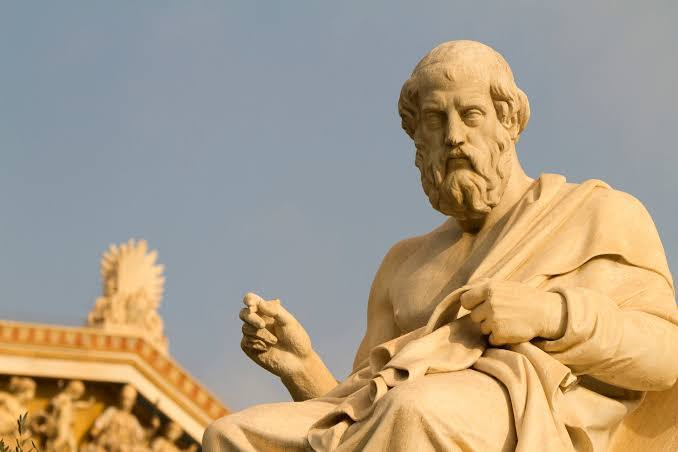
\includegraphics[width=1.5in]{images/plato.jpeg}
\caption*{\small ``Geometry is knowledge of the eternally existent… it compels the soul to look upwards, and leads us away from the world of appearance to the vision of truth.'' \\ ``Let no one ignorant of geometry enter here'' -- Plato}
\end{center}
\end{figure}


\begin{figure}[ht]
\centerline{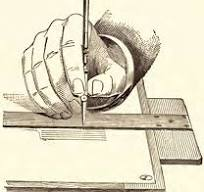
\includegraphics[width=2.0in]{images/straight.jpg}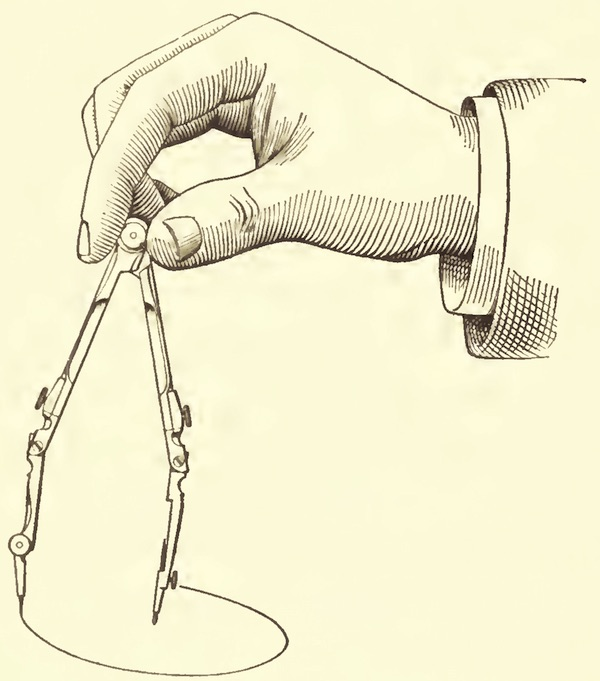
\includegraphics[width=2.0in]{images/compass.jpg}}
\caption{Ruler and compass. We will assume that the ruler is unmarked, and lengths can only be measured by adjusting the width of the compass.}
\label{fig:rulercompass}
\end{figure}

Our endeavour so far has been to define numbers, and operations on them, in a representation independent manner. Let us now consider a specific computational model -- \href{https://en.wikipedia.org/wiki/Straightedge\_and\_compass\_construction}{straightedge and compass constructions} introduced by the ancient Greeks -- and examine whether the abstract operations we have defined above can be translated in to definite constructible procedures, or {\em algorithms}. Most of the geometric constructions  date back to  \href{https://en.wikipedia.org/wiki/Euclid\%27s\_Elements}{Euclid's books of Elements} from around 300 BCE. We will often -- by force of habit -- refer to them as {\em ruler and compass constructions} but with the understanding that the ruler has no markings for length measurements, and can only be used to draw straight edges. See Figure \ref{fig:rulercompass}. 

Let us first consider some basic constructions. In what follows, the correctness of the constructions will often rely on the basic geometric properties of similar triangles. A reader may revise them from \href{https://en.wikipedia.org/wiki/Triangle}{here} and \href{https://en.wikipedia.org/wiki/Similarity\_(geometry)}{here}.

\section{Constructing a line perpendicular to a given line  passing through a point}
\label{sec:perp}
\begin{figure}
\begin{center}
\begin{tikzpicture}[scale=1.2]

% Draw circles
\draw(0,0) circle (1);
\draw (-1,0) circle (2);
\draw (1,0) circle (2);

% Draw horizontal line l
\draw[-] (-3.2,0) -- (3.2,0) node[right] {$\ell$};

% Draw vertical line through intersection
\draw[-] (0,-2.5) -- (0,2.5);

% Points A, x, B,a,b
\fill (-1,0) circle (2pt);
\fill (0,0) circle (2pt);
\fill (1,0) circle (2pt);
\fill (0,-1.72) circle (2pt);
\fill (0,1.72) circle (2pt);

% Labels (slightly below the line)
\node[below=4pt,left=1pt] at (-1,0) {$A$};
\node[below=4pt,right=1pt] at (0,0) {$x$};
\node[below=4pt,right=1pt] at (1,0) {$B$};
\node[above=4pt,right=0pt] at (0,1.8) {$a$};
\node[below=4pt,right=0pt] at (0,-1.8) {$b$};
\node[above=1pt] at (0.5,0) {$r$};

\end{tikzpicture}
\end{center}
\caption{Constructing a line perpendicular to a given line  passing through a point}
\label{fig:perp}
\end{figure}

Given a straight line $\ell$, and a point $x$ on it, let us consider the problem of constructing a line perpendicular to $\ell$ and passing through $x$. We give a construction  in Algorithm \ref{algo:perp}  (See Figure \ref{fig:perp}).
\begin{algorithm}
\begin{algorithmic}[1]
\Procedure{Perpendicular}{$x,\ell$}
\State $c = CIRCLE(x,r)$, where $r$ is a random length
\State $(A,B) = c \cap \ell$  
\State $c_A = CIRCLE(A,2r)$
\State $c_B = CIRCLE(B,2r)$
\State $(a,b) = c_A \cap c_B$
\State $result = LINE(a,b)$
\EndProcedure
\end{algorithmic}
\caption{Constructing a line perpendicular to a given line  passing through a point}
\label{algo:perp}
\end{algorithm}

We have described the algorithmic procedure using some standard primitives. $c = CIRCLE(x,r)$ denotes the construction of a circle $c$  centred at $x$ of radius $r$. $A$ and $B$ are the intersection points of $c$ with $\ell$, denoted in the algorithm as $(A,B) = c \cap \ell$. Similarly, $c_A$ and $c_B$ are circles of radius $2r$ centred at $A$ and $B$ respectively, and $a$ and $b$ are the intersection points of $c_A$ and $c_B$. $LINE(a,b)$ joins $a$ and $b$ and is the $result$.

\begin{exercise}
\begin{enumerate}
\item Convince yourself that the above construction is correct. Use properties of similar triangles.
\item Argue that $LINE(a,b)$ is also the perpendicular bisector of $AB$.
\end{enumerate}
\end{exercise}

\section{Constructing a line parallel to a given line  passing through a point}
\label{sec:parallel}
Given a line $\ell$, and an arbitrary point $x$, consider the problem of construction of a line parallel to $\ell$ passing through $x$. We give a construction  in Algorithm \ref{algo:parallel}  (See Figure \ref{fig:parallel}).

\begin{figure}
\begin{center}
\begin{tikzpicture}[line width=0.9pt, scale=1.2]

% ---- Parameters ----
\pgfmathsetmacro{\R}{2.2}   % circle radius
\pgfmathsetmacro{\h}{1.2}   % vertical offset from center to line \ell (positive)
\pgfmathsetmacro{\dx}{sqrt(\R*\R - \h*\h)} % half-chord length on \ell
\pgfmathsetmacro{\sx}{1.4}  % x-position of side guide lines (cosmetic)

% ---- Geometry ----
\coordinate (X) at (0,0);            % center of circle and label x
\coordinate (A) at (-\dx,-\h);       % left intersection with \ell
\coordinate (B) at ( \dx,-\h);       % right intersection with \ell
\coordinate (P) at (0,-\h);          % point on \ell vertically below x
\coordinate (Q) at (-\dx,0); 

% ---- Circle centered at x ----
\draw (X) circle (\R);

% ---- Horizontal lines: top through x, bottom \ell ----
\draw (-3,0) -- (3,0);                % top line through center
\draw (-3,-\h) -- (3,-\h);            % bottom line \ell
\node[left] at (-3,-\h) {$\ell$};

% ---- Vertical guides (left, center, right) ----
\draw (-\dx,-2.3) -- (-\dx,2.3);
\draw (0,-2.3) -- (0,2.3);
%\draw (\dx,-2.3) -- (\dx,2.3);

% ---- Points ----
\fill (A) circle (2pt);
\fill (B) circle (2pt);
\fill (P) circle (2pt);
\fill (X) circle (2pt);
\fill (Q) circle (2pt);

% ---- Labels (offset so they’re not on the lines) ----
\node[below left=4pt] at (X) {$x$};
\node[below left=4pt]  at (A) {$A$};
\node[below left=4pt]       at (P) {$P$};
\node[below left=4pt]       at (Q) {$Q$};
\node[below right=4pt] at (B) {$B$};

\end{tikzpicture}
\end{center}
\caption{Constructing a line parallel to a given line  passing through a point}
\label{fig:parallel}
\end{figure}

\begin{algorithm}
\begin{algorithmic}[1]
\Procedure{Parallel}{$x,\ell$}
\State $c = CIRCLE(x,r)$, where $r$ is a random length
\State $(A,B) = c \cap \ell$  
\State Construct $p$, the perpendicular bisector of $AB$ using Algorithm \ref{algo:perp}. Argue that $p$ passes through $x$.
\State $P = p \cap \ell$
\State Construct $q$, a perpendicular to $\ell$ passing through $A$ using Algorithm \ref{algo:perp}.
\State Construct $s$, a perpendicular to $p$ passing through $x$ using Algorithm \ref{algo:perp}.
\State $Q = q \cap s$
\State $result = LINE(Q,x)$
\EndProcedure
\end{algorithmic}
\caption{Constructing a line parallel to a given line  passing through a point}
\label{algo:parallel}
\end{algorithm}

Note that in steps 4,6 and 7 of the algorithm, we have used the procedure of Algorithm \ref{algo:perp}. We will routinely use a previously defined algorithm as a primitive to define a new algorithm.
\section{Constructibility and the compass equivalence theorem}

The above two sections give us several examples of construction of points, lines, line segments and circles. The informal definition of {\em constructibility} is as follows.  Given points are by definition constructible. A line joining two constructible points is constructible. So is the circle centred on one constructible point passing through another constructible point. A point is constructible if it is an intersection of constructible lines and circles.

The compass advocated by the Greek philosopher \href{https://en.wikipedia.org/wiki/Plato}{Plato} in these constructions is a {\em collapsing compass}, i.e., a compass that ``collapses'' whenever it is lifted from a page, so that it may not be directly used to transfer distances unlike in a modern fixable aperture compass. Note that nowhere in Sections \ref{sec:perp} and \ref{sec:parallel} have we transferred distances using a fixed size compass lifted from the page.

This is however not a limitation as the following construction shows.

\begin{theorem}
A collapsing compass can be used to transfer a given length to an arbitrary given point on a given line. That is, given an arbitrary length $\overline{AB}$, a line $\ell$ and a point $P$ on it, it is possible to construct using a collapsing compass a point $Q$ on $\ell$ such that $\overline{PQ} = \overline{AB}$.
\end{theorem}
\begin{proof}
\begin{figure}
\begin{center}
\includegraphics[width=0.5\textwidth]{rulercompass/no-collapse.png}

\end{center}
\caption{A compass-equivalence construction}
\label{fig:equiv}
\end{figure}

\begin{algorithm}
\begin{algorithmic}[1]
\Procedure{compass-equivalence}{$A$,$B$,$\ell$,$P$}
\State $c = CIRCLE(A,B)$; note that $\overline{AB} = d$
\State Construct $p$, the line parallel to $\ell$ passing through  $A$ using Algorithm \ref{algo:parallel}
\State $R = c \cap p$
\State $q = LINE(A,P)$
\State Construct $s$, the line parallel to $q$ passing through  $R$ using Algorithm \ref{algo:parallel}
\State $Q = s \cap \ell$
\State $\overline{PQ}$ is the result on $\ell$
\EndProcedure
\end{algorithmic}
\caption{A compass-equivalence construction}
\label{algo:equiv}
\end{algorithm}

\begin{exercise}
Convince yourself that $\overline{PQ} = \overline{AB}$.
\end{exercise}
\end{proof}

The above is different from the original construction and proof of correctness as given by Euclid in his Book of Elements. Interested readers may study a modern version of the original construction \href{https://en.wikipedia.org/wiki/Compass\_equivalence\_theorem}{here}.

\section{Rational numbers are constructible}

\begin{figure}
\begin{center}
\includegraphics[width=0.5\textwidth]{rulercompass/add.png}
\caption{Construction of $a+b$.}
\label{fig:add}
\end{center}
\end{figure}

\begin{figure}
\begin{center}
\includegraphics[width=0.5\textwidth]{rulercompass/sub.png}
\caption{Construction of $a-b$.}
\label{fig:sub}
\end{center}
\end{figure}

%\begin{figure}
%\begin{center}
%\includegraphics[width=0.5\textwidth]{rulercompass/mult.png}
%\caption{Construction of $ab$ given $a$ and $b$.}
%\label{fig:mult}
%\end{center}
%\end{figure}
%
%\begin{figure}
%\begin{center}
%\includegraphics[width=0.5\textwidth]{rulercompass/div.png}
%\caption{Construction of $a/b$ given $a$ and $b$.}
%\label{fig:div}
%\end{center}
%\end{figure}

% Multiplication: OA = a, OU = 1, OB = b, OX = ab.
\begin{figure}
\begin{center}
\begin{tikzpicture}[scale=1.1, line width=0.8pt]
    % Illustrative lengths: a = 1.8, b = 2.5.
    \coordinate (O) at (0,0);
    \coordinate (U) at (0,1);
    \coordinate (B) at (0,2.5);
    \coordinate (A) at (1.8,0);
    \coordinate (X) at (4.5,0);

    % Perpendicular lines through O.
    \draw (-0.15,0) -- (4.9,0) node[right] {$\ell$};
    \draw (0,-0.15) -- (0,2.85) node[above] {$m$};

    % AU and the parallel through B.
    \draw (U) -- (A);
    \draw (B) -- (X);

    % Right-angle mark.
    \draw (0,0.16) -- (0.16,0.16) -- (0.16,0);

    % Points and their auxiliary names.
    \foreach \P in {O,U,B,A,X}
        \fill (\P) circle (1.8pt);
    \node[below left=3pt] at (O) {$O$};
    \node[above right=3pt] at (U) {$U$};
    \node[above right=3pt] at (B) {$B$};
    \node[above right=3pt] at (A) {$A$};
    \node[above right=3pt] at (X) {$X$};

    % Vertical length markings.
    \draw[line width=0.5pt]
        (-0.30,0) -- (-0.30,1)
        node[midway,fill=white,inner sep=3pt] {$1$};
    \draw (-0.36,0) -- (-0.24,0);
    \draw (-0.36,1) -- (-0.24,1);

    \draw[line width=0.5pt]
        (-0.75,0) -- (-0.75,2.5)
        node[midway,fill=white,inner sep=3pt] {$b$};
    \draw (-0.81,0) -- (-0.69,0);
    \draw (-0.81,2.5) -- (-0.69,2.5);

    % Horizontal length markings.
    \draw[line width=0.5pt]
        (0,-0.40) -- (1.8,-0.40)
        node[midway,fill=white,inner sep=3pt] {$a$};
    \draw (0,-0.46) -- (0,-0.34);
    \draw (1.8,-0.46) -- (1.8,-0.34);

    \draw[line width=0.5pt]
        (0,-0.85) -- (4.5,-0.85)
        node[midway,fill=white,inner sep=3pt] {$ab$};
    \draw (0,-0.91) -- (0,-0.79);
    \draw (4.5,-0.91) -- (4.5,-0.79);
\end{tikzpicture}
\end{center}
\caption{Construction of $ab$ given $a$ and $b$.
Join $A$ to $U$ and draw the parallel through $B$,
meeting $\ell$ at $X$. Then $\overline{OX}=ab$.}
\label{fig:mult}
\end{figure}


% Division: OA = a, OB = b, OU = 1, OX = a/b.
\begin{figure}
\begin{center}
\begin{tikzpicture}[scale=1.1, line width=0.8pt]
    % Illustrative lengths: a = 4.5, b = 2.5.
    \coordinate (O) at (0,0);
    \coordinate (U) at (0,1);
    \coordinate (B) at (0,2.5);
    \coordinate (X) at (1.8,0);
    \coordinate (A) at (4.5,0);

    % Perpendicular lines through O.
    \draw (-0.15,0) -- (4.9,0) node[right] {$\ell$};
    \draw (0,-0.15) -- (0,2.85) node[above] {$m$};

    % AB and the parallel through U.
    \draw (B) -- (A);
    \draw (U) -- (X);

    % Right-angle mark.
    \draw (0,0.16) -- (0.16,0.16) -- (0.16,0);

    % Points and their auxiliary names.
    \foreach \P in {O,U,B,A,X}
        \fill (\P) circle (1.8pt);
    \node[below left=3pt] at (O) {$O$};
    \node[above right=3pt] at (U) {$U$};
    \node[above right=3pt] at (B) {$B$};
    \node[above right=3pt] at (X) {$X$};
    \node[above right=3pt] at (A) {$A$};

    % Vertical length markings.
    \draw[line width=0.5pt]
        (-0.30,0) -- (-0.30,1)
        node[midway,fill=white,inner sep=3pt] {$1$};
    \draw (-0.36,0) -- (-0.24,0);
    \draw (-0.36,1) -- (-0.24,1);

    \draw[line width=0.5pt]
        (-0.75,0) -- (-0.75,2.5)
        node[midway,fill=white,inner sep=3pt] {$b$};
    \draw (-0.81,0) -- (-0.69,0);
    \draw (-0.81,2.5) -- (-0.69,2.5);

    % Horizontal length markings.
    \draw[line width=0.5pt]
        (0,-0.40) -- (1.8,-0.40)
        node[midway,fill=white,inner sep=3pt] {$a/b$};
    \draw (0,-0.46) -- (0,-0.34);
    \draw (1.8,-0.46) -- (1.8,-0.34);

    \draw[line width=0.5pt]
        (0,-0.85) -- (4.5,-0.85)
        node[midway,fill=white,inner sep=3pt] {$a$};
    \draw (0,-0.91) -- (0,-0.79);
    \draw (4.5,-0.91) -- (4.5,-0.79);
\end{tikzpicture}
\end{center}
\caption{Construction of $a/b$ given $a$ and $b$, $b>0$.
Join $A$ to $B$ and draw the parallel through $U$,
meeting $\ell$ at $X$. Then $\overline{OX}=a/b$.}
\label{fig:div}
\end{figure}


First, we can consider any given length as 1, measure it using a non-collapsing compass -- which we just proved is equivalent to a collapsing compass -- and add it to any point on a given line by marking it off with the compass. We can similarly subtract. The operations $S(n)$ and $P(n)$ are thus realisable using ruler and compass. Consequently, the elements of the set $\Z$ are constructible. In Figures \ref{fig:add} and \ref{fig:sub} we give the direct constructions for $a+b$ and $a-b$.

Given integers $a$ and $b$ as line segments, we can also construct rational number $ab$ and $a/b$ directly using similar triangles. The construction of Figure \ref{fig:mult} involves marking off the lengths $a$ and $b$ in two perpendicular segments from $O$, constructing the unit length in the direction of $b$, and constructing a line parallel to the line $\overline{a1}$ through $a$ or $b$. The intercept of the parallel line in the direction of $a$ then marks  the length $ab$ by similarity of the triangles. We can similarly construct $a/b$ as depicted in Figure \ref{fig:div}. Rational numbers are thus constructible.  See the following Algorithms:

\begin{algorithm}
\begin{algorithmic}[1]
\Procedure{Multiply}{$a,b$}
\State Choose a horizontal line $\ell$ and a point $O$ on it
\State Construct $m$, the perpendicular to $\ell$ passing
       through $O$ using Algorithm \ref{algo:perp}
\State $c_a = CIRCLE(O,a)$
\State $A = c_a \cap \ell$, choosing the intersection
       to the right of $O$
\State $c_1 = CIRCLE(O,1)$
\State $U = c_1 \cap m$, choosing the intersection
       above $O$
\State $c_b = CIRCLE(O,b)$
\State $B = c_b \cap m$, choosing the intersection
       above $O$
\State $p = LINE(A,U)$
\State Construct $q$, the line parallel to $p$ passing
       through $B$ using Algorithm \ref{algo:parallel};
       if $B=U$, take $q=p$
\State $X = q \cap \ell$
\State $\overline{OX}$ is the result on $\ell$
\EndProcedure
\end{algorithmic}
\caption{Constructing $ab$ given $a$ and $b$}
\label{algo:mult}
\end{algorithm}

\begin{algorithm}
\begin{algorithmic}[1]
\Procedure{Divide}{$a,b$}
\State Choose a horizontal line $\ell$ and a point $O$ on it
\State Construct $m$, the perpendicular to $\ell$ passing
       through $O$ using Algorithm \ref{algo:perp}
\State $c_a = CIRCLE(O,a)$
\State $A = c_a \cap \ell$, choosing the intersection
       to the right of $O$
\State $c_b = CIRCLE(O,b)$
\State $B = c_b \cap m$, choosing the intersection
       above $O$
\State $c_1 = CIRCLE(O,1)$
\State $U = c_1 \cap m$, choosing the intersection
       above $O$
\State $p = LINE(A,B)$
\State Construct $q$, the line parallel to $p$ passing
       through $U$ using Algorithm \ref{algo:parallel};
       if $U=B$, take $q=p$
\State $X = q \cap \ell$
\State $\overline{OX}$ is the result on $\ell$
\EndProcedure
\end{algorithmic}
\caption{Constructing $a/b$ given $a$ and $b$, $b>0$}
\label{algo:div}
\end{algorithm}

\begin{exercise}
\begin{enumerate}
\item Describe a ruler and compass procedure for multiplication using repeated additions.
\item Describe a ruler and compass procedure for division (computing quotient and remainder) using repeated subtractions.
\end{enumerate}
\end{exercise}



\section{Euclid's GCD using ruler and compass}
\label{sec:gcd}
GCD of two integers $a > 0$, $b \geq 0$ is defined as the largest integer $d, d > 0$ that divides both $a$ and $b$. Consider the following algorithm for computing the GCD:
        \[
                gcd(a,b)
                 = \left\{      \begin{array}{ll}
                                a       &                     \mbox{if $b = 0$} \\
                                a       &                     \mbox{if $a = b$} \\
                                gcd(a-b,b)      &       \mbox{if $a > b$} \\
                                gcd(a,b-a)      &       \mbox{if $b > a$}
                                \end{array}
                        \right.
        \]
\begin{exercise}
\begin{enumerate}
\item        Convince yourself that the above algorithmic specification (rule) is correct for computing GCD. Carry out the pencil and paper computation using the  above algorithm for some  special cases.
\item         Describe the procedure for executing the algorithm using ruler and compass.
\end{enumerate}
\end{exercise}

The algorithm described above is from Euclid's Elements. You can find a description of it \href{https://en.wikipedia.org/wiki/Euclidean_algorithm}{here}. This is also considered to be the oldest non-trivial algorithm in common use.

Now that we have defined our first computational model, several questions arise. What are the full powers of the model? What are the other things that can be constructed? What are the limits of the model, and are there easily defied concepts that are not constructible? Can there be other computational models more powerful than ruler and compass?  These are the kind of questions we interrogate every computational model with. We will revisit some of these questions in the latter chapters.

\begin{exercise}
\label{exer:squarerootof2}
 Try to construct $\sqrt{2}$ using ruler and compass. (Hint: Use the Pythagoras theorem 
  on a right triangle with sides $1, 1$.) Argue why this length is constructible.
  \label{exer:sqrt2}
\end{exercise}


\section*{Problems}

\begin{enumerate}
  %\setcounter{enumi}{4}

  \item Construct, using ruler and compass, the perpendicular bisector of a line segment $AB$. 
  Show that any point $P$ on the perpendicular bisector is equidistant from $A$ and $B$.

  \item Given a triangle $ABC$, construct the three medians using ruler and compass. 
  Argue that they intersect at a single point (the centroid).  

  \item Using Algorithm~3 (perpendicular construction), describe step by step how to construct 
  the altitude from a vertex of a triangle. Illustrate your steps with a figure.

  \item Given a line $\ell$ and an external point $P$, use Algorithm~4 (parallel construction) 
  to draw the line parallel to $\ell$ through $P$. Prove that the two lines do not intersect.

  \item Show that the compass-equivalence construction (Algorithm~5) indeed allows one to 
  transfer a given length $AB$ to an arbitrary point $P$ on a line $\ell$. 
  Verify your construction with a worked example.

  \item Describe a ruler and compass procedure for multiplication of two integers $a, b$ 
  using repeated additions. Demonstrate the construction for $a=3, b=4$.

  \item Similarly, describe a ruler and compass procedure for division using repeated subtractions. 
  Apply your method to compute the quotient and remainder when dividing a segment of length $11$ 
  into parts of length $3$.

  \item Using constructions based on similar triangles, show step by step how to obtain 
  the product $ab$ given line segments $a$ and $b$.

  \item Construct the rational number $\tfrac{3}{5}$ on a line, starting with a unit segment. 
  Explain each step of your construction.

  \item Apply Euclid’s GCD algorithm (as given in Section 3.5) to the lengths $a = 21$, $b = 15$, 
  using repeated subtraction with compass and ruler. Show all intermediate steps.

  \item Prove that Euclid’s GCD algorithm terminates in a finite number of steps for all $a, b \in \mathbb{N}$. 
  (Hint: in each step one of the arguments strictly decreases.)

   

\end{enumerate}


\chapter{Abstraction turns problems and concepts into principles}
\label{chap:relationsandfunctions}


\begin{figure}[ht]
\centerline{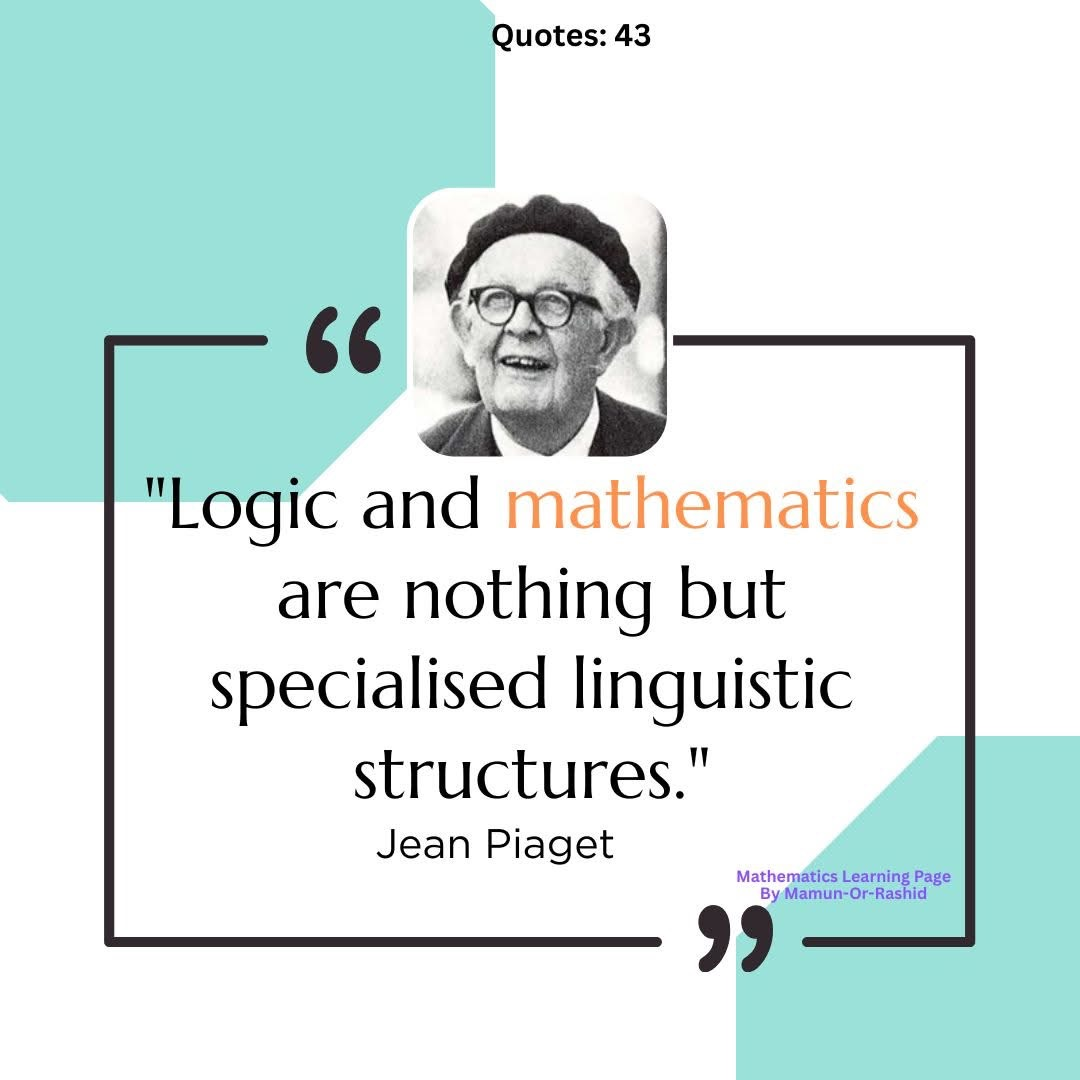
\includegraphics[width=2.0in]{images/piaget.jpg}}
\end{figure}

Modern mathematics and computer science are built upon a few simple but very powerful ideas. 
Among the most important are the notions of \emph{relations} and \emph{functions}, which 
allow us to describe how objects are connected or transformed. 
Counting, infinity, and the ways in which sets can be grouped into classes 
help us measure size, structure, and complexity. 
These ideas may look abstract at first, but they underlie the methods used 
in algorithms, data structures, and logical reasoning.

In computer science, functions capture the essence of computation: 
a program takes inputs and produces outputs, just as a function does. 
Understanding one-one and onto functions helps us reason about 
whether information is lost, preserved, or fully covered. 
Equivalence classes and partitions allow us to organise data into categories. 
Modular arithmetic, often called ``clock arithmetic,'' is fundamental 
in cryptography, error detection, and digital systems. 
Learning these concepts gives us a foundation to explore deeper 
mathematics and to apply it to practical computational problems.

\section{Relations}

The {\em Cartesian product} of two sets $A$ and $B$, denoted by
$A \times B$, is the set of all ordered pairs $(a,b)$ such that
$a \in A$ and $b \in B$. Thus,
\[
A \times B = \{(a,b) \mid (a \in A) \mbox{ and } (b \in B)\}
\]
$A^n$ is the set of all ordered $n$-tuples $(a_1,a_2,\ldots,a_n)$
such that $a_i \in A$ for all $i$. i.e.,
\[
A^n = \underbrace{A \times A \times \cdots \times A}_{n \mbox{ times}}
\]


A \emph{relation} tells us which elements of one set are connected to elements of another.

A {\em binary relation} $R$ from $A$ to $B$ is a subset of $A \times B$. It is
a characterisation of the intuitive notion that some of the elements of $A$ 
are related to some of the elements of $B$. 

If $A=\{1,2,3\}$ and $B=\{a,b,c\}$, then
$R=\{(1,a),(2,b),(3,a)\}$ is a relation from $A$ to $B$.
Familiar binary relations from
$\N$ to $\N$ are $=,\;\neq,\;<,\;\leq,\;>,\;\geq$. Thus the elements
of the set $\{(0,0),(0,1),(0,2),\ldots,(1,1),(1,2),\ldots\}$ are all members
of the relation $\leq$ which is a subset of $\N \times \N$.

\begin{figure}
\begin{center}
\begin{tikzpicture}[>=Stealth, node distance=10mm]
  % Left: relation that is not a function
  \node[draw, rounded corners, minimum width=3.2cm, minimum height=3.6cm,label=above:{\footnotesize Relation (not a function)}] (L) {};
  \node (A1) at ([xshift=-1.1cm,yshift=1.0cm]L.center) {$1$};
  \node (A2) at ([xshift=-1.1cm,yshift=0.0cm]L.center) {$2$};
  \node (A3) at ([xshift=-1.1cm,yshift=-1.0cm]L.center) {$3$};
  \node (B1) at ([xshift=1.1cm,yshift=1.0cm]L.center) {$a$};
  \node (B2) at ([xshift=1.1cm,yshift=0.0cm]L.center) {$b$};
  \node (B3) at ([xshift=1.1cm,yshift=-1.0cm]L.center) {$c$};
  \draw[->] (A1) -- (B1);
 % \draw[->] (A1) .. controls +(-0.2,-0.5) and +(0.2,0.5) .. (B2); % two outputs from 1
  \draw[->] (A1) -- (B2);
  \draw[->] (A2) -- (B3);

  % Right: valid function
  \node[draw, rounded corners, minimum width=3.2cm, minimum height=3.6cm, right=2.8cm of L,label=above:{\footnotesize Function}] (R) {};
  \node (C1) at ([xshift=-1.1cm,yshift=1.0cm]R.center) {$1$};
  \node (C2) at ([xshift=-1.1cm,yshift=0.0cm]R.center) {$2$};
  \node (C3) at ([xshift=-1.1cm,yshift=-1.0cm]R.center) {$3$};
  \node (D1) at ([xshift=1.1cm,yshift=1.0cm]R.center) {$a$};
  \node (D2) at ([xshift=1.1cm,yshift=0.0cm]R.center) {$b$};
  \node (D3) at ([xshift=1.1cm,yshift=-1.0cm]R.center) {$c$};
  \draw[->] (C1) -- (D1);
  \draw[->] (C2) -- (D2);
  \draw[->] (C3) -- (D2);
\end{tikzpicture}
\end{center}
\caption{Relation vs function: In a relation, an element in $A$ can be mapped to multiple elements in $B$, but not so in a function. In a function, all elements in $A$ must be covered, but not necessarily so in a relation. The set $B$ need not be fully covered in either. }
\label{fig:relationvsfunction}
\end{figure}

\section{Function}
A \emph{function} from $A$ to $B$ -- written as $f: A \to B$ -- is a special relation in which:
\begin{enumerate}
  \item every element of $A$ is related to some element of $B$, and
  \item no element of $A$ is related to more than one element of $B$.
\end{enumerate}
Equivalently, each input has \emph{exactly one} output. 

Some familiar examples of functions are 
\begin{enumerate}
\item   $+$ and $*$ (addition and multiplication) are functions of the type
        $f: \N \times \N \rightarrow \N$ 
\item   $-$ (subtraction) is a function of the type $f: \N \times \N \rightarrow
 \Z$.
\item   $div$ and $mod$ are functions of the type $f: \N \times \N \rightarrow \N$.
        If $a = q*b + r$ such that $0 \leq r < b$ and $a,b,q,r \in \N$ then
        the functions $div$ and $mod$ are defined as $div(a,b) = q$ and
        $mod(a,b) = r$. We will often write these binary functions as
        $a * b$, $a\; div \;b$, $a \; mod \; b$ etc.
\item   The binary relations $=,\;\neq,\;<,\;\leq,\;>,\;\geq$ are also functions of the type
        $f: \N \times \N \rightarrow \B$        where $\B = \{false,true\}$.
\item $f:\N\to\N,\ f(x)=x^2$.
\end{enumerate}


We write the definition of a function formally as follows.

A {\em function} from $A$ to $B$ is a binary relation $f$ from $A$ to $B$ such
that for {\em every} element $a \in A$ there is a {\em unique} element
$b \in B$ so the $(a,b) \in f$ (or $f(a) = b$)\footnote{This is sometimes written using mathematical notation as $\forall a \in A$, $\exists$ unique $b \in B$. $\forall$ is the usual symbol for {\em for all}, and $\exists$ is the usual symbol for {\em there exists}}. We will use the notation 
$f: A \rightarrow B$
to denote a function $f$ from $A$ to $B$. The set $A$ is called the 
{\em domain} of the function $f$ and the set $B$ is called the {\em co-domain}
of the function $f$. The {\em range} of a function $f: A \rightarrow B$ is the
set $\{b \in B \mid \mbox{for some $a \in A$, $f(a) = b$}\}$ denoting the subset of elements in $B$ that are actually covered by $f$. 


\subsection{One-One (injective), Onto (surjective), and bijective Functions}
When we study functions, it is often not enough to know that “every input has exactly one output.”
We also want to understand how well the function uses its codomain and whether different inputs remain distinct after applying the function.

Think of a classroom with students and seats:
\begin{itemize}
\item If no two students sit in the same seat, the “assignment” of students to seats is one-one (injective).
\item If every seat is occupied by at least one student, the assignment is onto (surjective).
\item If both conditions happen together — each student has exactly one seat, and every seat is filled — then the assignment is bijective. In such a case we may also define an inverse  function from seats to students.
\end{itemize}

\begin{figure}
\begin{center}
\begin{tikzpicture}[>=Stealth, node distance=8mm]
  % Injective not surjective
  \node[draw, rounded corners, minimum width=3.4cm, minimum height=3.6cm,label=above:{\footnotesize Injective, not surjective}] (I) {};
  \node (i1) at ([xshift=-1.2cm,yshift=1.0cm]I.center) {$1$};
  \node (i2) at ([xshift=-1.2cm,yshift=0.0cm]I.center) {$2$};
  \node (i3) at ([xshift=-1.2cm,yshift=-1.0cm]I.center) {$3$};
  \node (u1) at ([xshift=1.2cm,yshift=1.2cm]I.center) {$a$};
  \node (u2) at ([xshift=1.2cm,yshift=0.4cm]I.center) {$b$};
  \node (u3) at ([xshift=1.2cm,yshift=-0.4cm]I.center) {$c$};
  \node (u4) at ([xshift=1.2cm,yshift=-1.2cm]I.center) {$d$};
  \draw[->] (i1) -- (u1);
  \draw[->] (i2) -- (u2);
  \draw[->] (i3) -- (u3);
  % u4 is empty -> not surjective

  % Surjective not injective
  \node[draw, rounded corners, minimum width=3.4cm, minimum height=3.6cm, right=3.2cm of I,label=above:{\footnotesize Surjective, not injective}] (S) {};
  \node (s1) at ([xshift=-1.2cm,yshift=1.0cm]S.center) {$1$};
  \node (s2) at ([xshift=-1.2cm,yshift=0.0cm]S.center) {$2$};
  \node (s3) at ([xshift=-1.2cm,yshift=-1.0cm]S.center) {$3$};
  \node (v1) at ([xshift=1.2cm,yshift=0.6cm]S.center) {$a$};
  \node (v2) at ([xshift=1.2cm,yshift=-0.6cm]S.center) {$b$};
  \draw[->] (s1) -- (v1);
  \draw[->] (s2) -- (v1);
  \draw[->] (s3) -- (v2);

  % Bijective
  \node[draw, rounded corners, minimum width=3.4cm, minimum height=3.6cm, right=3.2cm of S,label=above:{\footnotesize Bijective}] (B) {};
  \node (b1) at ([xshift=-1.2cm,yshift=1.0cm]B.center) {$1$};
  \node (b2) at ([xshift=-1.2cm,yshift=0.0cm]B.center) {$2$};
  \node (b3) at ([xshift=-1.2cm,yshift=-1.0cm]B.center) {$3$};
  \node (w1) at ([xshift=1.2cm,yshift=1.0cm]B.center) {$a$};
  \node (w2) at ([xshift=1.2cm,yshift=0.0cm]B.center) {$b$};
  \node (w3) at ([xshift=1.2cm,yshift=-1.0cm]B.center) {$c$};
  \draw[->] (b1) -- (w1);
  \draw[->] (b2) -- (w2);
  \draw[->] (b3) -- (w3);
\end{tikzpicture}
\end{center}
\caption{{\em One-one (injective)}: different inputs give different outputs. (like roll numbers: no two students share one roll); {\em Onto (surjective)}: every element of the codomain gets hit by \emph{some} input. (no empty seats.); {\em Bijective}: both one-one and onto. (perfect pairing; has an inverse.)}
\end{figure}


The formal definitions below make the concepts precise.

Let $f:A \to B$ be a function. $f$ is 
\begin{description}
  \item[Injective]  if whenever  $f(a_1)=f(a_2)$ for $a_1, a_2 \in A$, we can conclude that $a_1 = a_2$
  \item[Surjective]  if for all $b \in B$, there exists $a \in A$ such that $f(a)=b$.
  \item[Bijective] if it is both injective and surjective.
\end{description}

\begin{example}
\begin{enumerate}
  \item $f:\N \to \R,\ f(n)=2n$ is injective but not surjective (odd numbers are not covered).
  \item $g:\N \to\N,\ g(0)=0;\;g(n)=n-1$  is surjective but not injective (why?).
 \end{enumerate}
 \end{example}
 
 \section{Counting, Finite and Infinite Sets}

Counting is one of the most fundamental activities in mathematics: it is how we measure the 
size of a set. At first glance this seems very straightforward — counting  laddoos in a box
or students in a class is familiar to everyone. However, mathematics asks us to extend this 
simple idea to more abstract settings: What does it mean for a set to be ``finite''? 
How can we formally compare the sizes of different sets, especially when some sets are 
infinite? For finite sets, the answer is clear: we can match the elements of the set 
to the numbers $\{1,2,\dots,n\}$. For infinite sets, the situation is more subtle, but 
surprisingly we can still talk about ``countable'' sets — those whose elements can be placed 
in a one-to-one correspondence with the natural numbers $\N$. This point of view leads to 
some striking and important results: for instance, that the set of all even numbers, the 
set of all integers, and even the set of all rational numbers are all countably infinite. 
At the same time,  we will see later in this course that there are sets of  numbers  so large that they cannot even be 
listed in sequence: these are called uncountable sets. These distinctions between finite, 
countably infinite, and uncountable sets form the foundation for much of modern mathematics, 
and are crucial in computer science as well, where questions of size, encoding, and 
enumeration play a central role.

\subsection{Finite sets}
A set is \emph{finite} if it has a finite number of elements.
Formally, a set $A$ is finite if there exists a natural number $n$ and a bijection
\[
f: A \to \{1,2,\dots,n\}.
\]
This means that the elements of $A$ can be paired exactly with the first $n$ natural numbers.

\begin{example}
The set $\{a,b,c\}$ is finite because we can define $f(a)=1$, $f(b)=2$, $f(c)=3$,
which is a bijection to $\{1,2,3\}$.
\end{example}

\subsection{Infinite sets and bijections to $\N$}
A set is \emph{infinite} if it is not finite. Some infinite sets are still ``countable''
because they can be put in one-to-one correspondence (bijection) with the natural numbers $\N$.  In such a case the elements of the set can be enumerated as {\em first}, {\em second}. {\em third}, and so on.

\paragraph{Definition.} 
A set $A$ is \emph{countably infinite} or {\em denumerable} if there exists a bijection $f:A\to\N$.

\begin{example}
\begin{enumerate}
\item The natural numbers $\N$ are countably infinite via the trivial bijection $f(n)=n$.
\item The set of even naturals $E=\{0,2,4,6,\dots\}$ is countably infinite. Define $f:\N\to E$ by $f(n)=2n$. This is a bijection.
\item The set of odd naturals $O=\{1,3,5,7,\dots\}$ is also countably infinite. Define $g:\N\to O$ by $g(n)=2n+1$. This is a bijection.
\end{enumerate}
\end{example}

\subsection{Integers and Rationals are countable}

The integers $\Z=\{\dots,-2,-1,0,1,2,\dots\}$ can be enumerated in a sequence:
\[
0,-1,1,-2,2,-3,3,-4,4,\dots
\]
Define a bijection $h:\N\to\Z$ by
\[
h(n) = \begin{cases}
\phantom{-}\tfrac{n}{2} & \text{if $n$ is even},\\[6pt]
-\tfrac{n+1}{2} & \text{if $n$ is odd}.
\end{cases}
\]
This shows that $\Z$ is countable.

The rationals $\Q=\{\tfrac{p}{q}: p,q\in\Z, q\neq 0\}$ are also countable, though the proof
is less obvious.

\paragraph{Step 1.} First, consider only the positive rationals $\Q^+$.
We can arrange them in a grid with numerator along one axis and denominator along the other:
\[
\begin{array}{c|cccc}
 & 1 & 2 & 3 & \dots \\
\hline
1 & \tfrac{1}{1} & \tfrac{1}{2} & \tfrac{1}{3} & \dots \\
2 & \tfrac{2}{1} & \tfrac{2}{2} & \tfrac{2}{3} & \dots \\
3 & \tfrac{3}{1} & \tfrac{3}{2} & \tfrac{3}{3} & \dots \\
\vdots & \vdots & \vdots & \vdots & \ddots
\end{array}
\]
Note, however, that this does not give us an enumeration.

\paragraph{Step 2.} Use \href{https://en.wikipedia.org/wiki/Georg\_Cantor}{Cantor}’s  method:
start at $\tfrac{1}{1}$, then $\tfrac{2}{1},\tfrac{1}{2}$, then $\tfrac{3}{1},\tfrac{2}{2},\tfrac{1}{3}$,
and so on, zig-zagging across the grid. This produces a sequence that eventually lists every positive rational.

\begin{tikzpicture}[>=Stealth, every node/.style={inner sep=1pt}]
  % grid size
  \def\M{5}

  % grid border and lines
  %\draw[very thin] (0.5,0.5) rectangle (\M+0.5,\M+0.5);
  %\foreach \x in {1,...,\M} \draw[very thin] (\x,0.5) -- (\x,\M+0.5);
  %\foreach \y in {1,...,\M} \draw[very thin] (0.5,\y) -- (\M+0.5,\y);

  % axis labels
  \node[below=2mm] at (\M/2+0.5,0.5) {$q$ (denominator)};
  \node[rotate=90,left=2mm] at (0.5,\M/2+0.5) {$p$ (numerator)};

  % place p/q labels at grid nodes: node Npq at (q, M+1-p)
  \foreach \p in {1,...,\M}{
    \foreach \q in {1,...,\M}{
      \node (N\p\q) at (\q,\M+1-\p) {\scriptsize $\frac{\p}{\q}$};
    }
  }

  % Cantor zig-zag sequence (first 15 terms) and successive arrows
  \def\seq{1/1, 2/1, 1/2, 3/1, 2/2, 1/3, 4/1, 3/2, 2/3, 1/4, 5/1, 4/2, 3/3, 2/4, 1/5}

  \newcount\step
  \step=0
  \def\prevnode{}
  \foreach \p/\q in \seq {
    \advance\step by 1
    % draw arrow from previous node to current node
    \ifx\prevnode\empty
    \else
      \draw[-{Stealth[length=2mm]}] (\prevnode) -- (N\p\q);
    \fi
    % dot and step number near the node
    \fill (N\p\q) circle (0.02);
    %\node[font=\tiny, fill=white, inner sep=0.4pt] at ([xshift=1.8mm,yshift=1.8mm] N\p\q) {\the\step};
    % update previous node
    \xdef\prevnode{N\p\q}
  }
\end{tikzpicture}

\begin{exercise}
\begin{enumerate}
\item Convince yourself that above ordering gives a bijection from $\N$ to ordered pairs $(p,q), p > 0, q > 0$.
\item Can you work out an explicit formula for the bijective function? ({\bf This can be challenging})
\end{enumerate}
\end{exercise}

\paragraph{Step 3.} To avoid repetitions, we can restrict to fractions in lowest terms
(e.g.\ $\tfrac{2}{2}$ is skipped since it equals $\tfrac{1}{1}$).

\paragraph{Step 4.} To cover negative rationals as well, interleave them with positives:
\[
0, \tfrac{1}{1}, -\tfrac{1}{1}, \tfrac{2}{1}, -\tfrac{2}{1}, \tfrac{1}{2}, -\tfrac{1}{2}, \dots
\]

This construction defines an explicit enumeration of $\Q$,
so $\Q$ is countably infinite.

\section{Equivalence Relations, Classes, and Partitions}

In mathematics, we often want to group objects together when they share some common property. 
For example,  in geometry all shapes that have the same size and shape are considered ``congruent,'' 
and in number theory two integers that leave the same remainder when divided by $n$ are considered ``equivalent.''  
These situations are captured formally by the concept of an \emph{equivalence relation}.  

Equivalence relations are important because they let us partition a large and possibly complicated set 
into smaller, simpler pieces (called \emph{equivalence classes}). Each equivalence class collects 
all elements that are considered ``the same'' under the relation. Many areas of mathematics, 
and even computer science (e.g.\ hashing, classification, state-space reduction), rely on such partitions.

\paragraph{Definition.} 
A relation $R$ on a set $A$ is an \emph{equivalence relation} if for all $a,b,c\in A$:
\begin{itemize}
  \item (Reflexive) $(a,a)\in R$,
  \item (Symmetric) $(a,b)\in R \Rightarrow (b,a)\in R$,
  \item (Transitive) $(a,b)\in R$ and $(b,c)\in R \Rightarrow (a,c)\in R$.
\end{itemize}
We will also write $(a,b) \in R$ as $a\; R \; b$ or as $a \sim b$. 

\paragraph{Definition.} 
Set of elements that are equivalent form an {\emph equivalent class}.  Given $a \in A$, the \emph{equivalence class} of $a$ under relation $R$ is
\[
[a] = \{ x \in A : (a,x)\in R \}.
\]


Here are some example of equivalent relations
\begin{example}
\begin{enumerate}

 \item \textbf{Same birthday.}  
  On the set of all students, define $x \sim y$ if $x$ and $y$ have the same birthday.  
  Each equivalence class is a group of students born on the same day.  
  
  \item \textbf{Congruent triangles.}  
  On the set of all triangles in the plane, define $T_1 \sim T_2$ if $T_1$ and $T_2$ are congruent 
  (same shape and size). This relation is reflexive (every triangle is congruent to itself), 
  symmetric (if $T_1$ is congruent to $T_2$, then $T_2$ is congruent to $T_1$), 
  and transitive (if $T_1$ is congruent to $T_2$ and $T_2$ to $T_3$, then $T_1$ is congruent to $T_3$).  
  

\item \textbf{Sets with same cardinality.}
Clearly, $A \sim B$ if there exists a bijection between $A$ and $B$. Since bijective functions have inverses that are bijections, and composition of two bijective functions is a bijection, we have
that sets with same cardinality for an equivalent class.
  
  \item \textbf{Congruence of integers (mod $n$).}  
  Define $a \sim b$ if $n$ divides $a-b$.  We write this as $a \sim b\pmod{n}$ or $a \equiv b\pmod{n}$.
  This is reflexive ($a-a=0$ is divisible by $n$), symmetric (if $a-b$ divisible by $n$, so is $b-a$), 
  and transitive (if $a-b$ and $b-c$ divisible by $n$, so is $a-c$).  
  The equivalence classes are the sets of integers with the same remainder when divided by $n$.
  
  For example, on a $12$-hour clock, $16\sim 4\pmod{12}$; and, for the minutes hand, $65\sim 5\pmod{60}$;
  
  \begin{center}
  \begin{tikzpicture}[scale=2]
  % Draw the clock circle
  \draw[thick] (0,0) circle(1);

  % Place hour numbers
  \foreach \num in {1,...,12} {
    \node at ({90-30*\num}:0.85) {\num};
  }

  % Minute hand (5 minutes -> at "1")
  \draw[thick, red] (0,0) -- ({90-30*1}:0.7);

  % Hour hand (4 hours + 5 minutes -> 4*30 + 2.5 = 122.5 degrees clockwise)
  \draw[thick, blue] (0,0) -- ({90-(4*30+2.5)}:0.5);

  % Center dot
  \fill (0,0) circle(0.03);
\end{tikzpicture}
\end{center}
\end{enumerate}
\end{example}

\begin{exercise}
Which of the following relations are not equivalent relations and why?
\begin{enumerate}
\item $a\;R\;b$ if $a = b$.
\item $a\;R\;b$ if $a \leq b$.
\item $a\;R\;b$ if $gcd(a,b) = 1$.
\end{enumerate}
\end{exercise}

\subsection{Equivalence classes and partitions}
\label{sec:eq-classes}

\begin{theorem}
An equivalence relation defined on  set $A$  {\emph partitions} $A$ into disjoint equivalence classes: every element of $A$ belongs 
to exactly one equivalence class, and the classes together cover all of $A$.
\end{theorem}

\begin{proof}
We have to argue for two things -- first, no element belongs to two or more equivalent classes; and second, the union of all the equivalence classes covers the whole set.

Suppose $x$ belongs to two distinct equivalence classes. Then there exits $a,b \in A$ such that $x \sim a$ and $x \sim b$ but $a \not \sim b$. But this is not possible because $\sim$ is symmetric and transitive.

And, by reflexivity, each $x$ is at least equivalent to itself. So, no element is left out.
\end{proof}

\begin{example}
The relation Congruence of integers (mod $3$)  split $\Z$  into three classes:
\[
[0] = \{\dots,-6,-3,0,3,6,\dots\}, \quad
[1] = \{\dots,-5,-2,1,4,7,\dots\}, \quad
[2] = \{\dots,-4,-1,2,5,8,\dots\}.
\]
These three classes form a partition of $\Z$.
\end{example}

\section{Modular Arithmetic, Magic Squares, and One-Time Pads}
\label{sec:modular}

\subsection{Modular arithmetic}
Consider, for example, the set $\mathbb{Z}_7 = \{0,1,2,3,4,5,6\}$ consists of all integers modulo $7$. 
This means that we can perform addition and multiplication, and then reduce the result 
to its remainder upon division by $7$.

\paragraph{Addition.}
Examples:
\[
3 + 5 \equiv 1 \pmod{7}, \quad 6 + 4 \equiv 3 \pmod{7}.
\]

Every element has an \emph{additive inverse}, i.e.\ a number $x$ such that 
$a + x \equiv 0 \pmod{7}$. We denote this as $x \equiv a^{-1} \pmod{7}$
\[
0^{-1} \equiv 0 \pmod{7},\quad 1^{-1} \equiv 6 \pmod{7}, \quad 2^{-1} \equiv 5, \pmod{7},\quad 3^{-1} \equiv 4 \pmod{7},.
\]

\paragraph{Multiplication.}
Examples:
\[
3 \times 5 \equiv 1 \pmod{7}, \quad 4 \times 6 \equiv 3 \pmod{7}.
\]
For multiplication, every nonzero element has a \emph{multiplicative inverse}, 
i.e.\ $a \cdot x \equiv 1 \pmod{7}$.
\[
1^{-1} \equiv 1 \pmod{7},\quad 2^{-1} \equiv 4 \pmod{7},\quad 3^{-1} \equiv 5 \pmod{7},,\quad 6^{-1} \equiv 6 \pmod{7},.
\]
Notice that $0$ has no multiplicative inverse.

Thus $(\mathbb{Z}_7, +)$ is a finite arithmetic structure under addition, 
and $(\mathbb{Z}_7^\times,\cdot)$ with $\{1,2,3,4,5,6\}$ is a finite arithmetic structure under multiplication. This has many interesting applications.

\subsection{Magic Squares}
A \emph{magic square} is an arrangement of numbers in a square grid such that the sums of each row, column, 
and both diagonals are the same. Modular arithmetic allows us to construct magic squares 
in structures like $\mathbb{Z}_n$, where the “magic sum” is computed modulo $n$.  
This is a playful illustration of modular addition applied to combinatorial design. 

A simple way to build a magic square \emph{modulo $n$} is to take any ordinary magic square
and reduce each entry modulo $n$. The \href{https://en.wikipedia.org/wiki/Luoshu\_Square}{LuoShu $3\times 3$ square}, which has a rich history in occult and numerology is given as
\[
\begin{array}{|c|c|c|}
\hline
4 & 9 & 2 \\
\hline
3 & 5 & 7 \\
\hline
8 & 1 & 6 \\
\hline
\end{array}
\qquad\text{(each line sums to $15$)}
\]
It reduces modulo $7$ to
\[
\begin{array}{|c|c|c|}
\hline
4 & 2 & 2 \\
\hline
3 & 5 & 0 \\
\hline
1 & 1 & 6 \\
\hline
\end{array}
\quad\in\; \mathbb{Z}_7^{\,3\times 3}.
\]
Since $15\equiv 1\pmod{7}$, every row, column, and diagonal now sums to $\overline{1}\in\mathbb{Z}_7$.
For instance,
\[
4+2+2 \equiv 8 \equiv 1 \pmod{7},\qquad
3+5+0 \equiv 8 \equiv 1 \pmod{7},\qquad
1+5+2 \equiv 8 \equiv 1 \pmod{7}.
\]
The diagonals also satisfy $4+5+6\equiv 15\equiv 1\pmod{7}$ and $2+5+1\equiv 8\equiv 1\pmod{7}$.

\paragraph{General recipe (odd moduli).}
Let $S$ be any $3\times 3$ magic square over the integers with magic sum $M$.
For any modulus $n\ge 2$, the entry-wise reduction $\overline{S}\in(\mathbb{Z}_n)^{3\times 3}$ is a
magic square in $\mathbb{Z}_n$ with magic sum $\overline{M}\in\mathbb{Z}_n$,
because modular addition preserves equality of sums. More generally, for any $\alpha,\beta\in\mathbb{Z}_n$,
the entry-wise  transform $\alpha S+\beta$ is again a magic square modulo $n$ with magic sum
$\alpha M+3\beta \pmod{n}$.

\subsection{Perfect Secrecy and One-Time Pads}
The idea of modular arithmetic is also central in cryptography.  
In the \emph{one-time pad}, a message (plaintext) is converted into numbers 
(say letters $A=0,\dots,Z=25$). A random secret key of the same length is chosen, 
and encryption is done by addition modulo $26$:
\[
\text{ciphertext}_i \equiv \text{plaintext}_i + \text{key}_i \pmod{26}.
\]
Decryption uses subtraction modulo $26$.  

Claude Shannon showed that if the key is truly random, used only once, and kept secret, 
then the ciphertext reveals no information about the plaintext: this is called 
\emph{perfect secrecy}. Thus, a simple application of modular addition gives us 
a theoretically unbreakable cryptosystem.

\subsection*{Summary}
Modular arithmetic provides the framework to work with remainders in a structured way. 
It underlies recreational mathematics like magic squares, as well as fundamental 
cryptographic protocols such as the one-time pad.


\section*{Problems}

\begin{enumerate}

  \item Let $A = \{1,2,3\}$ and $B = \{a,b,c\}$.  
  (a) List all elements of the Cartesian product $A \times B$.  
  (b) Define two different binary relations $R_1, R_2 \subseteq A \times B$.  
  (c) Which of them, if any, are functions?

  \item Show that the relation $\leq$ on $\mathbb{N}$ is a subset of $\mathbb{N} \times \mathbb{N}$.  
  Explicitly write out the first ten elements of this relation.

  \item Give an example of a relation from $\{1,2,3\}$ to $\{a,b\}$ that is not a function.  
  Explain why it fails to satisfy the definition of a function.

  \item Consider the function $f : \mathbb{N} \to \mathbb{N}$ defined by $f(n) = 2n$.  
  Argue that $f$ is injective but not surjective.  

  \item Consider the function $g : \mathbb{N} \to \mathbb{N}$ defined by  
  \[
    g(0) = 0, \qquad g(n) = n-1 \ \text{for } n > 0.
  \]
  Show that $g$ is surjective but not injective.  

  \item Let $h : \mathbb{Z} \to \mathbb{Z}$ be defined by $h(x) = x+5$.  
  Prove that $h$ is bijective and describe its inverse function.

  \item Define the function $p : \mathbb{N} \times \mathbb{N} \to \mathbb{N}$ by $p(a,b) = a \times b$.  
  Argue formally that $p$ is a well-defined function.

  \item Construct an example of a function $f : A \to B$ where $A = \{1,2,3,4\}$, $B = \{a,b\}$ 
  that is neither injective nor surjective. Explain why.

  \item Prove that if a function $f : A \to B$ is bijective, then there exists a unique inverse 
  function $f^{-1} : B \to A$ such that $f^{-1}(f(a)) = a$ for all $a \in A$.  

  \item Consider the function $f : \mathbb{N} \to \mathbb{N}$ defined recursively as  
  \[
    f(0) = 0, \quad f(n+1) = f(n) + (2n+1).
  \]
  Show that $f(n) = n^2$. What kind of function is this (injective, surjective, bijective)?  

  \item Give an everyday example (outside mathematics) of:  
  (a) an injective mapping,  
  (b) a surjective mapping, and  
  (c) a bijective mapping.  

  \item Challenge: Prove or disprove — the composition of two injective functions is injective, 
  and the composition of two surjective functions is surjective. What about bijective functions?  
  
  % Equivalence relations
  \item On the set $\{1,2,3,4,5,6\}$, define a relation $R$ by $a \sim b$ if $a-b$ is divisible by $2$. 
        \begin{enumerate}
            \item Show that $R$ is an equivalence relation.
            \item List the equivalence classes.
        \end{enumerate}

  \item Consider the relation ``$x$ has the same number of letters as $y$'' on the set of English words.
        Prove or disprove that it is an equivalence relation. What do the equivalence classes look like?

  % Modular arithmetic
  \item Work out the addition and multiplication tables of $\mathbb{Z}_5$. Identify all additive and multiplicative inverses.

  \item In $\mathbb{Z}_7$, solve the linear congruence $3x \equiv 2 \pmod{7}$.

  \item Find all solutions to $x^2 \equiv 1 \pmod{15}$. 

  % Bijections and countability
  \item Construct a bijection between the set of even numbers and $\mathbb{N}$. 
        Then, using a diagram, show how integers $\mathbb{Z}$ can be listed in sequence, proving that they are countable.

%  \item Use Cantor’s diagonal method to prove that the real numbers in $[0,1]$ are uncountable. Illustrate with a decimal expansion example.

  \item Show that the set of rational numbers $\mathbb{Q}$ is countable by describing an explicit enumeration strategy.

  % Magic squares and applications
  \item Verify that the LuoShu square
        \[
        \begin{array}{|c|c|c|}
        \hline
        4 & 9 & 2 \\
        \hline
        3 & 5 & 7 \\
        \hline
        8 & 1 & 6 \\
        \hline
        \end{array}
        \]
        is a magic square. What is its magic sum?

  \item Construct a $3\times 3$ magic square modulo $7$ using the method of reducing an ordinary magic square.
        What is the magic sum in $\mathbb{Z}_7$?

  % Cryptography
  \item In a one-time pad over the alphabet $\{A=0,B=1,\dots,Z=25\}$, encrypt the message 
        \texttt{MATH} with the key \texttt{CODE}. 
        Show the numerical steps modulo $26$ and give the ciphertext.

  \item Explain why re-using the same key in a one-time pad scheme can destroy perfect secrecy. 
        Give a simple example with short  strings.


\end{enumerate}

\chapter{We need precision in thought and action to win arguments}
\label{chap:logicandproofs}


\begin{figure}[ht]
\centerline{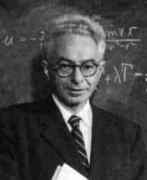
\includegraphics[width=1.0in]{images/courant.jpg}}
\caption*{\small ``Mathematics as an expression of the human mind reflects the active will, the contemplative reason, and the desire for aesthetic perfection. Its basic elements are logic and intuition, analysis and construction, generality and individuality.'' -- Richard Courant}
\end{figure}

\begin{figure}[ht]
\centerline{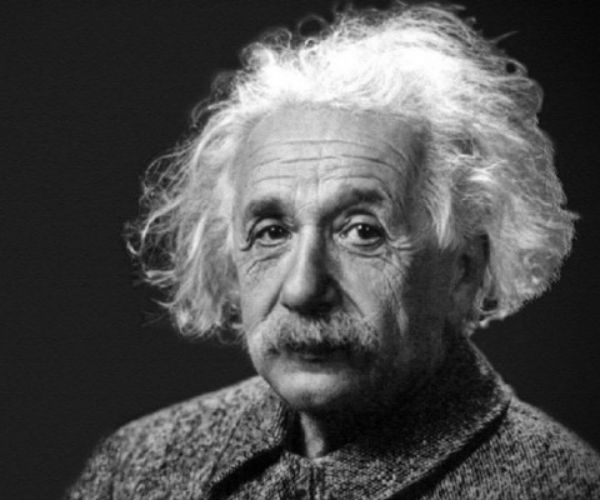
\includegraphics[width=1.0in]{images/einstein.jpeg}}
\caption*{\small ``Pure mathematics is, in its way, the poetry of logical ideas.'' -- Albert Einstein}
\end{figure}


Logic is the language of reasoning. Whenever we argue in mathematics, 
make a claim in science, or even decide something in everyday life, 
we  implicitly use the rules of logic. Boolean logic, named after the mathematician \href{https://en.wikipedia.org/wiki/George\_Boole}{George Boole}, 
provides a precise mathematical framework to study truth and falsity. 

In this chapter, we will introduce the basic building blocks of logic, 
learn how to represent them with truth tables, explore important rules like De Morgan’s laws, 
understand how to work with more than two statements at a time, 
and examine subtle but important ideas such as vacuous truth. 
Equally importantly, we will also study some of the standard methods of writing mathematical proofs. 
These include direct proofs, proofs by counter-examples, proofs by contrapositive, proofs by contradiction, 
and proofs by induction. Learning these strategies will allow you to apply logical reasoning 
to establish mathematical results with clarity and rigour.  

The aim of this chapter is to provide a foundation that is both rigorous and intuitive, 
preparing you for deeper study in mathematics and computer science, 
where careful reasoning and proof techniques are essential.

\section{Propositions, Basic Boolean Logic and Truth Tables}

In mathematics and computer science, many problems boil down to deciding whether something
is \emph{true} or \emph{false}.  
A statement that can be judged true or false is called a \emph{proposition}.  
For example:
\begin{itemize}
  \item ``2 is an even number'' is true.
  \item ``5 is less than 3'' is false.
  \item ``$x+2=7$'' is a proposition, but its truth depends on the value of $x$.
\end{itemize}

Boolean logic studies how we can combine such statements using logical operations 
like \textbf{AND}, \textbf{OR}, \textbf{NOT}, and \textbf{IMPLIES}.  
These operations are the foundation of digital circuits, programming languages, 
and formal mathematical proofs.

\subsection{The basic operations}
We denote truth values as T (true) and F (false).

\paragraph{Conjunction (AND).} 
The statement $p \land q$ is true only if both $p$ and $q$ are true.  
\emph{Example:} ``I will go for a walk \emph{and} it is sunny.''  
This is only true if both parts are true.

\paragraph{Disjunction (OR).}
The statement $p \lor q$ is true if at least one of $p$ or $q$ is true.  
\emph{Example:} ``I will have tea \emph{or} coffee.''  
In everyday language, ``or'' can sometimes mean ``one but not both,'' 
but in logic the inclusive sense is used: tea, coffee, or both makes the statement true.

\paragraph{Negation (NOT).}
The statement $\lnot p$ has the opposite truth value of $p$.  
\emph{Example:} If $p=$``It is raining,'' then $\lnot p=$``It is not raining.''

\paragraph{Implication (IF...THEN).}
The statement $p \Rightarrow q$ means ``$p$ implies $q$'' or ``If $p$ then $q$.''  
It is false only when $p$ is true but $q$ is false.  
In all other cases it is true.  
Think of it as a promise:  
``If you pass the QRMT course, then you will get a laddoo.''\footnote{Note, however, that I am making no such promise. It is just a supposition for making a point.} The only way the promise fails is if you pass but still do not get a laddoo.  
If (unfortunately) you do not pass, the promise is not broken if you still get a laddoo, so the implication is considered true. Passing QRMT is sufficient to get a laddoo, so we say that ``$p$ is {\em sufficient} for $q$''. Passing the course and yet not getting a laddoo will make the promise false, so we say that ``$q$ is {\em necessary} for $p$''.

\paragraph{Biconditional (IF AND ONLY IF).}
The statement $p \Leftrightarrow q$ is true when both  $p \Rightarrow q$ and  $q \Rightarrow p$, i.e., $p$ and $q$ have the same truth value, 
either both true or both false.  
\emph{Example:} ``A number is even if and only if it is divisible by 2.''

\paragraph{Exclusive OR (XOR).}
The statement $p \oplus q$ is true when exactly one of $p$ or $q$ is true, but not both.  
\emph{Example:} ``You can win first prize \emph{or} second prize.''  
You cannot win both at the same time.

\subsection{Truth tables}
Truth tables let us list all possible truth values of statements and see how the logical operations work.

\begin{center}
\begin{tabular}{|c|c||c|c|c|c|c|}
\hline
$p$ & $q$ & $p \land q$ & $p \lor q$ & $p \Rightarrow q$ & $p \Leftrightarrow q$ & $p \oplus q$ \\
\hline
T & T & T & T & T & T & F \\
T & F & F & T & F & F & T \\
F & T & F & T & T & F & T \\
F & F & F & F & T & T & F \\
\hline
\end{tabular}
\end{center}

\subsubsection{De Morgan’s Laws}
These laws explain how negation interacts with AND and OR:
\[
\lnot(p \land q) \equiv (\lnot p) \lor (\lnot q), 
\qquad
\lnot(p \lor q) \equiv (\lnot p) \land (\lnot q).
\]

\begin{example} 
Let $p=$``bring a wizard to the QRMT class'' $q=$``bring a dragon to the QRMT class''  
Then $\lnot(p \lor q)$ means ``do not bring a wizard or a dragon to the QRMT class,''  
which is the same as ``do not bring a wizard to the QRMT class {\em and} do not bring a dragon to the QRMT class''.
\end{example}
\begin{example}
In contrast,  $\lnot(p \land q)$  means  ``It is not the case that you bring both a wizard and a dragon to the QRMT class,'' which is logically equivalent to ``either you do not bring a wizard to the QRMT class \emph{or} you do not bring a dragon to the QRMT class (or both).''
\end{example}

\begin{exercise}
\begin{enumerate}
\item Convince yourself that the truth functions given in the table above, and the De Morgan's laws, are reasonable.
\item In particular, it is the truth table of $p \Rightarrow q$ that is most commonly used in logical deductions. Try to think of a few example English sentences that corroborate the truth table; especially the third row.
\item Argue, using both truth tables and language-based examples, that $p \Rightarrow q$ is equivalent to $\lnot q \Rightarrow \lnot p$. This is called {\em contrapositive}.
\item Argue, using both truth tables and language-based examples, that $p \Rightarrow q$ is equivalent to $\lnot p \lor q$.
\item Argue, using both truth tables and language-based examples, that $p \Leftrightarrow q$ is equivalent to $\lnot (p \oplus q)$.
\item Sometimes, in everyday life, we observe $q$, and hypothesize $p$ and $p \Rightarrow q$, i.e., we hypothesize that $p$ may have caused $q$. This is called {\emph abductive reasoning}.  Argue that such abductive reasoning will violate our rules of deduction in mathematics. However, abductive reasoning is essential for the sciences and the social sciences. Can you reason why, perhaps through some examples? The hypotheses generated through abductive reasoning of course need to be validated, even in the sciences and the social sciences.
\end{enumerate}
\label{exer:truthexers}
\end{exercise}

The truth tables that underlie propositional logic are not empirical discoveries but conventions inherited from linguistic and philosophical traditions. They represent a form of “agreed upon truth,” codifying how we collectively interpret connectives such as “and,” “or,” “not,” and ``implies." In this sense they are {\em axiomatic} in nature: we do not prove that $\lnot (p \lor q)$ should behave like $(\lnot p \land \lnot q)$, we simply accept the tabular assignments as the foundation upon which deductions are made. Logical proofs then proceed within this framework of shared agreement. If any one of us refuses to accept these conventions — if, for example, someone insists that “and,” “or,” or ``implies" should work differently — then there is no common ground to move forward, and the very possibility of building logical arguments collapses.

\subsection{Three-variable examples of truth tables}
When we have three propositions $p,q,r$, there are $2^3 = 8$ possible combinations 
of truth values. Truth tables become longer, but the method is the same.

\paragraph{Example 1.} 
Consider $p \land (q \lor r)$.  
We first compute $q \lor r$, then combine with $p$ using AND.

\begin{center}
\begin{tabular}{|c|c|c||c|c|}
\hline
$p$ & $q$ & $r$ & $q \lor r$ & $p \land (q \lor r)$ \\
\hline
T & T & T & T & T \\
T & T & F & T & T \\
T & F & T & T & T \\
T & F & F & F & F \\
F & T & T & T & F \\
F & T & F & T & F \\
F & F & T & T & F \\
F & F & F & F & F \\
\hline
\end{tabular}
\end{center}



\paragraph{Example 2.}
Consider $(p \Rightarrow q) \land (q \Rightarrow r)$.  
This corresponds to chaining two implications: 
``If $p$ then $q$, and if $q$ then $r$.''

\begin{center}
\begin{tabular}{|c|c|c||c|c|c|}
\hline
$p$ & $q$ & $r$ & $p \Rightarrow q$ & $q \Rightarrow r$ & $(p \Rightarrow q)\land(q \Rightarrow r)$ \\
\hline
T & T & T & T & T & T \\
T & T & F & T & F & F \\
T & F & T & F & T & F \\
T & F & F & F & T & F \\
F & T & T & T & T & T \\
F & T & F & T & F & F \\
F & F & T & T & T & T \\
F & F & F & T & T & T \\
\hline
\end{tabular}
\end{center}

\subsubsection{Venn diagram illustration}
The formula $p \land (q \lor r)$ can also be illustrated with sets. 
Think of $p,q,r$ as sets of outcomes where each proposition is true. 
The shaded area corresponds to outcomes where $p$ is true \emph{and} 
at least one of $q$ or $r$ is true.

\begin{center}
\begin{tikzpicture}[scale=1.3, thick]
  % circle radius and centers
  \def\r{1.2}
  \coordinate (P) at (0,0);
  \coordinate (Q) at (1.3,0.7);
  \coordinate (R) at (1.3,-0.7);

  % --- Shade P ∩ (Q ∪ R): clip to P, then fill Q and R ---
  \begin{scope}
    \clip (P) circle (\r);
    \fill[gray!35] (Q) circle (\r);
    \fill[gray!35] (R) circle (\r);
  \end{scope}

  % outlines
  \draw (P) circle (\r);
  \draw (Q) circle (\r);
  \draw (R) circle (\r);

  % labels for sets
  \node[left]  at ($(P)+(-0.9,0.9)$) {$p$};
  \node[right] at ($(Q)+(0.9,0.9)$) {$q$};
  \node[right] at ($(R)+(0.9,-0.9)$) {$r$};

  % universe box (optional)
  \draw[-, thin] ($(P)+(-1.8,-2)$) rectangle ($(Q)+(1.8,2)$);

  % title (optional)
  \node[below=6pt] at ($(P)!0.5!(Q)$) {$\;p \land (q \lor r)\;$};
\end{tikzpicture}
\end{center}

\section{Vacuous Truth}

The third line of the truth table for $p \Rightarrow q$, which suggests that if $p$ is {\em false} and $q$ is {\em true}, then   $p \Rightarrow q$ is {\em true}, requires special attention. This forms the basis for
many subtle logical arguments.
A statement of the form ``If $p$ then $q$'' is called an implication.  
As we saw, an implication is only false if $p$ is true and $q$ is false.  
Therefore, if $p$ is false, the implication is always true.  
This phenomenon is called \emph{vacuous truth}.  

\begin{example}
\begin{enumerate}
  \item ``If $5$ is even, then $5$ is prime.''  
        Since $5$ is not even, the whole statement is true, regardless of the second part.
  \item ``All unicorns have wings.''  
        This can be written as ``For every $x$, if $x$ is a unicorn then $x$ has wings.''  
        Since there are no unicorns, the condition never applies, and so the statement is vacuously true.
  \item ``If I am the king of France, then $2+2=5$.''  
        Because the condition ``I am the king of France'' is false, the implication is true.
\end{enumerate}
\end{example}

Vacuous truth is not a trick — it is a necessary feature of logic.  
It ensures that statements of the form ``All elements of an empty set have property $P$'' 
are automatically true.  
For example: ``All prime numbers greater than $1000$ and less than $1001$ are even.''  
There are no such numbers, so the statement is vacuously true. 

We will use this quite a bit in the latter chapters.

\section{Mathematical proofs}

A proof is a method for establishing the truth of a statement.  We use different methods in different spheres of life:

\begin{table}[h]
\centering
\begin{tabular}{|c|c|c|c|}
\hline
Rigour & Truth type & Field & Truth teller  \\
\hline
0 & Word of God        & Religion          & God/Priests \\
1 & Authoritative truth & Business/School & Boss/Teacher \\
2 & Legal truth         & Judiciary         & Law/Judge/Lawmakers \\
3 & Philosophical truth & Philosophy        & Plausible argument \\
4 & Scientific truth    & Physical sciences & Experiments/Observations \\
5 & Statistical truth   & Statistics        & Data sampling \\
6 & Mathematical truth  & Mathematics       & Logical deduction \\
\hline
\end{tabular}
%\caption{Different types of ``truth'' as presented on the slide ``What is a proof?''}
\end{table}
Mathematical reasoning applies the highest standards of rigour for what may be considered as a {\em proof}, but only for very tightly defined domains.
In mathematics we do not accept statements as true merely because  they seem plausible or reasonable, or because many examples seem to support them. A \emph{proof} is a logically complete argument that establishes truth from agreed assumptions, which may be definitions, axioms, or previously proved results. This chapter presents some core proof techniques, each with its own “feel’’ and natural use cases:
\begin{enumerate}
\item \textbf{Proof by Explicit Construction} — to prove that an element with some qualifying property exists, it is sufficient to construct an example.
\item \textbf{Proof by Counter-Example} — to disprove a universal claim, find one instance where it fails.
  \item \textbf{Direct Proof} — derive the conclusion straight from the hypothesis using definitions and algebra.
   \item \textbf{Proof by Contrapositive} — prove the logically equivalent statement \(\neg Q \Rightarrow \neg P\) instead of \(P \Rightarrow Q\).
  \item \textbf{Proof by Contradiction} — assume the negation of what you want, reach an impossibility, and conclude the original claim.
  \item \textbf{Proof by the Pigeonhole Principle} — to prove using the principle that if more objects are placed into fewer containers, then at least one container must hold more than one object.
  \item \textbf{Proof by exhaustion of cases} — prove that statement hold for all of an exhaustive set of cases.
   \item \textbf{Proof by Induction} — prove a base case and a step that carries truth from \(n\) to \(n{+}1\). 
   \item \textbf{Proof of equivalence} -- prove $P \; \Longleftrightarrow \;  Q$.
\end{enumerate}
Along the way, we emphasize \emph{how} to think when choosing a technique.

\subsection{Proof by Explicit Construction}

A \emph{proof by explicit construction} demonstrates the truth of a statement of
the form ``there exists $x$ such that $P(x)$'' by actually exhibiting such an
$x$ and verifying that it satisfies $P(x)$. This is perhaps the most concrete
kind of existence proof: instead of reasoning abstractly, we build or display
the required object \footnote{In ancient Mesopotamia (ca 2000 BCE), Babylonian mathematicians used algorithmic procedures to solve linear and quadratic equations for specific examples. The ancient Greeks -- most notably Euclid (ca 300 BCE) --  introduced geometric construction as a core part of geometric proofs. The ku\d{t}\d{t}aka (pulverizer) algorithm of \={A}ryabha\d{t}a ($5^{th}$ c) ($5^{th}$ c), Jayadeva (c. $10^{th}$–$11^{th}$ c.), and later Bh\'{a}skara II ($12^{th}$ c.) is a direct construction of integer solutions to linear Diophantine equations. Before the $19^{th}$ century most proofs were constructive in nature.}.

In our earlier discussion of \emph{ruler and compass} constructions in Section \ref{sec:rulerandcompasqs} we showed,
step by step, how to construct a length $a+1$ from a given length $a$, or how
to realize the greatest common divisor of two numbers geometrically. Each of
those is an instance of explicit construction: the proof of existence of a
geometric object lies in the instructions themselves.

Here are some other examples of proof by explicit construction. 

\begin{theorem}
There exist integers $x,y$ such that $14x+21y=7$.
\end{theorem}
\begin{proof}
We explicitly construct one such solution: take $x=-1$, $y=1$. Then
\[
14(-1)+21(1)=-14+21=7.
\]
Thus such integers exist. In fact, by varying $x$ and $y$ we can generate an
infinite family of solutions, but the single explicit example suffices to
establish existence.
\end{proof}

\begin{theorem}
There exist integers $a,b,c$ such that $a^2+b^2=c^2$.
\end{theorem}
\begin{proof}
Exhibit $(a,b,c)=(3,4,5)$. Indeed,
\[
3^2+4^2=9+16=25=5^2.
\]
Hence such integers exist. This triple is explicitly constructed and is known
as the smallest nontrivial Pythagorean triple.
\end{proof}

\begin{theorem}
For any rationals $r<s$, there exists a rational $q$ with $r<q<s$.
\end{theorem}
\begin{proof}
Explicitly construct $q=\tfrac{r+s}{2}$. Because $r<s$, we clearly have
$r<q<s$. Moreover, since $r$ and $s$ are rational, their average $q$ is also
rational. Thus such a $q$ exists.
\end{proof}

\begin{theorem}
\label{thm:diaphontine}
There exist integers $x,y$ such that
\[
35x + 22y = 1.
\]
\end{theorem}

\begin{proof}
To construct a solution, we compute the greatest common divisor of $35$ and $22$.

\begin{align*}
35 &= 1\cdot 22 + 13, \\
22 &= 1\cdot 13 + 9, \\
13 &= 1\cdot 9 + 4, \\
9 &= 2\cdot 4 + 1.
\end{align*}

Now back-substitute to express $1$ as a combination of $35$ and $22$:

\[
1 = 9 - 2\cdot 4.
\]

But $4 = 13 - 1\cdot 9$, so
\[
1 = 9 - 2(13-9) = 3\cdot 9 - 2\cdot 13.
\]

Now substitute $9 = 22 - 13$:
\[
1 = 3(22-13) - 2\cdot 13 = 3\cdot 22 - 5\cdot 13.
\]

Next, substitute $13 = 35 - 22$:
\[
1 = 3\cdot 22 - 5(35-22) = -5\cdot 35 + 8\cdot 22.
\]

Thus, one explicit solution is
\[
x=-5,\quad y=8.
\]
\end{proof}

\paragraph{Remark.}
Equations such as above are called {\em linear Diophantine equations}. A solution may not always exist. The above method of finding a solution if it exists  is called the {\em Extended Euclidean algorithm}, which not only proves that solutions exist when 
$\gcd(35,22)=1$, but by working through the steps we explicitly \emph{construct}
the solution \footnote{The origins of this algorithm can be traced back to the {\bf ku\d{t}\d{t}aka} (pulverizer) algorithm of \={A}ryabha\d{t}a ($5^{th}$ c), Jayadeva (c. $10^{th}$–$11^{th}$ c.) and later Bh\'{a}skara II ($12^{th}$ c.) refined and applied the ku\d{t}\d{t}aka extensively. Bh\'{a}skara in the L\={\i}l\={a}vat\={\i} and B\={\i}jaga\d{n}ita gives worked examples of solving linear Diophantine equations with what is recognizably the extended Euclid method.}.


\begin{theorem}
The integer $5$ has a multiplicative inverse modulo $17$.
\end{theorem}

\begin{proof}
We need an integer $x$ such that
\[
5x \equiv 1 \pmod{17}.
\]

This is equivalent to solving the linear Diophantine equation
\[
5x + 17y = 1
\]
for integers $x,y$.

Apply the Euclidean algorithm:
\begin{align*}
17 &= 3\cdot 5 + 2, \\
5  &= 2\cdot 2 + 1.
\end{align*}

Now back-substitute:
\[
1 = 5 - 2\cdot 2.
\]

But $2 = 17 - 3\cdot 5$, so
\[
1 = 5 - 2(17 - 3\cdot 5) = 7\cdot 5 - 2\cdot 17.
\]

Thus
\[
1 = 7\cdot 5 + (-2)\cdot 17,
\]
which shows that $x=7$, $y=-2$ is an explicit solution.

Therefore
\[
5\cdot 7 \equiv 1 \pmod{17},
\]
so $7$ is the multiplicative inverse of $5$ modulo $17$.
\end{proof}

\paragraph{Remark.}
This construction not only proves that $5$ has an inverse modulo $17$, but also
produces the explicit inverse $7$. In fact, the extended Euclidean algorithm
always gives such a construction whenever $\gcd(a,m)=1$.

\paragraph{When to prove by explicit construction.}
Proof by explicit construction is particularly valuable when the question is
``does there exist?'' and the object in question is concrete enough to build or
write down. It contrasts with nonconstructive methods (such as contradiction or
pigeonhole arguments, which we will study later) where existence is established without showing a specific
example. Both are mathematically valid, but constructive proofs have the added
advantage of providing insight into the nature of the object itself.


\subsection{Proof by Counter-Example}
A universal statement \(\forall x\, P(x)\) is false if there exists a single \(x\) with \(\neg P(x)\). Producing such an \(x\) \emph{disproves} the claim completely \footnote{Philosophically and logically, the concept of a counterexample existed in ancient Greek dialectics and argumentation, notably in the Socratic method where contradictory examples were used to challenge general claims or definitions. In medieval and early modern mathematics, counterexamples became more systematically used to falsify conjectures. Famous historical examples include \href{https://en.wikipedia.org/wiki/Fermat\_number}{Euler’s counterexample disproving the conjecture that all Fermat numbers are prime}.}. For example, consider the exchange of Figure \ref{fig:twitter} on social media

\begin{figure}[h]
\centerline{
\includegraphics[width=2.5in]{images/counterexample.jpg}}
\caption{A counter-example to a universal claim}
\label{fig:twitter}
\end{figure}

\begin{exercise}
Which basic logical reasoning method has been used here to disprove the universal claim?
\end{exercise}


\begin{example}
Let us consider a few more examples.
\begin{enumerate}
\item  {\bf Claim}: ``The product of any two prime numbers is prime.'' \newline
\noindent\textbf{Counter-example.} \(2\cdot 3=6\) is not prime.

\item {\bf Claim}: ``For all integers \(n\), the number \(n^2+n+41\) is prime.'' \newline
\noindent\textbf{Counter-example.} At \(n=41\), \(41^2+41+41=41\cdot 43\) is composite.

\end{enumerate}
\end{example}
.

\begin{figure}[h]
\begin{center}
\begin{tikzpicture}[every node/.style={font=\small}]
  % universal claim as circle
  \node[draw, circle, minimum size=3cm] (U) {$\forall x$ has property $P(x)$};

  % good elements inside
  \node[draw, circle, fill=black, inner sep=1.6pt, xshift=-1cm, yshift=0.8cm] (a) {};
  \node[draw, circle, fill=black, inner sep=1.6pt, xshift=0.5cm, yshift=-0.6cm] (b) {};

  % counterexample
  \node[draw, circle, fill=white, inner sep=1.6pt, very thick, xshift=0.8cm, yshift=0.8cm] (c) {};
 % \node[above right=8.5mm of c] {$x^\star$ with $\neg P(x^\star)$};

  % arrow explanation
  \draw[-{Latex}] (c) -- ++(1.2,0.2) node[right]{\begin{minipage}{2.5cm} $x^\star$ with $\neg P(x^\star)$ disproves the universal claim \end{minipage}};
\end{tikzpicture}
\end{center} 
\caption{One counterexample $x^\star$ inside the ``universe’’ circle shows the claim $\forall x \, P(x)$ is false.}
\end{figure}

\paragraph{What counter-examples teach.}
They refine sloppy universal claims. When a statement fails, analyzing \emph{why} the witness breaks it  often suggests a corrected statement. The expression $n^2 + n + 41$ produces prime numbers for all integers $n$ with $0 \le n \le 39$, but fails afterwards. 

\subsection{Direct Proof}
A direct proof of \(P \Rightarrow Q\) proceeds as a straight line: \(\text{Assume }P \;\rightarrow\) unpack definitions \(\rightarrow\) algebra/logic \(\rightarrow Q\).

Consider the following examples.

\paragraph{Definition.}
An integer \(n\) is \emph{even} if \(n=2k\) for some integer \(k\); it is \emph{odd} if \(n=2k+1\) for some integer \(k\).


\begin{theorem}\label{thm:even+even}
If \(a\) and \(b\) are even integers, then \(a+b\) is even.
\end{theorem}
\begin{proof}
Let \(a=2k\) and \(b=2m\) for integers \(k,m\). Then
\[
a+b=2k+2m=2(k+m),
\]
which is a multiple of \(2\), hence even.
\end{proof}

\begin{theorem}
If \(x\) is odd, then \(x^2\) is odd.
\end{theorem}
\begin{proof}
Let \(x=2k+1\). Then \(x^2=(2k+1)^2=4k^2+4k+1=2(2k^2+2k)+1\), which is odd.
\end{proof}

\begin{theorem}
$1 + 2 + 3 + \cdots + n  = n(n+1)/2$
\end{theorem}
\begin{proof}
Let $S = 1 + 2 + 3 + \cdots + n$. \\
Hence,  $S = n + (n-1) + (n-2) + \cdots + 1$,  in the reverse order. This implies that 
\[
2S = \underbrace{(n+1) + (n+1) + (n+1) + \cdots + (n+1)}_{\mbox{$n$ times}}
\]
Thus, $S = n(n+1)/2$.
\end{proof}

\begin{theorem}
Every odd integer is equal to the difference between the squares of two integers.
\end{theorem}
\begin{proof}
Let $a = 2k+1$ be an arbitrary odd integer. Then $a = 2k + 1 = k^2 + 2k + 1 -k^2 = (k+1)^2 - k^2$.
\end{proof}

\begin{theorem}
An integer $n$ is divisible by $3$ $\;\Longleftrightarrow\;$ the sum of its digits is divisible by $3$.
\end{theorem}

\begin{proof}
Write $n$ in decimal expansion as
\[
n = d_0 + 10d_1 + 10^2 d_2 + \cdots + 10^k d_k,
\]
where $d_0, d_1, \dots, d_k$ are the digits of $n$.

Since $10 \equiv 1 \pmod{3}$, it follows that
\[
10^i \equiv 1 \pmod{3} \quad \text{for every } i \geq 0.
\]
Therefore
\[
n \equiv d_0 + d_1 + \cdots + d_k \pmod{3}.
\]

%\textbf{($\Rightarrow$)} Suppose $n$ is divisible by $3$. Then $n \equiv 0 \pmod{3}$.
%But $n \equiv d_0+d_1+\cdots+d_k \pmod{3}$. Hence the digit sum is also
%congruent to $0$ modulo $3$, i.e. divisible by $3$.
%
%\textbf{($\Leftarrow$)} Conversely, suppose the digit sum is divisible by $3$.
%Then $d_0+d_1+\cdots+d_k \equiv 0 \pmod{3}$. Since $n \equiv d_0+\cdots+d_k \pmod{3}$, it follows that $n \equiv 0 \pmod{3}$, i.e. $n$ is divisible by $3$.
\end{proof}


\begin{theorem}
Let $n$ be a positive integer with decimal form $n=10q+u$, where $u$ is the units digit
and $q$ is the number formed by the remaining digits. Then
\[
n \text{ is divisible by } 7 \;\;\Longleftrightarrow\;\; q-2u \text{ is divisible by } 7.
\]
\end{theorem}

\begin{proof}
Working modulo $7$, note first that $10\equiv 3\pmod{7}$, hence
\[
n=10q+u \equiv 3q+u \pmod{7} \equiv 3(q-2u) + 7u \pmod{7}  \equiv  3(q-2u)  \pmod{7}
\]

Since $3$ is invertible modulo $7$ (indeed $3^{-1}\equiv 5\pmod{7}$), we have
\[
3q+u \equiv 0 \pmod{7} \;\Longleftrightarrow\; q-2u \equiv 0 \pmod{7}.
\]
Combining with $n \equiv 3q+u \pmod{7}$ yields
\[
n \equiv 0 \pmod{7} \;\Longleftrightarrow\; q-2u \equiv 0 \pmod{7}.
\]
%Then,
%\textbf{($\Rightarrow$)} If $n$ is divisible by $7$, then $n \equiv 0 \pmod{7}$.
%Hence $q - 2u \equiv 0 \pmod{7}$, i.e., $q - 2u$ is divisible by $7$.
%
%\textbf{($\Leftarrow$)} Conversely, if $q - 2u$ is divisible by $7$, then
%$q - 2u \equiv 0 \pmod{7}$. Since $n \equiv q - 2u \pmod{7}$, it follows that
%$n \equiv 0 \pmod{7}$, i.e., $n$ is divisible by $7$.

\end{proof}

\paragraph{Example.}
For $n=483$ we have $q=48$, $u=3$, so $q-2u=48-6=42$, a multiple of $7$. Hence $483$ is divisible by $7$.

\begin{exercise} 
Argue that for bigger numbers, the test can be applied repeatedly by computing  $q-2u$ on the result.
\end{exercise}


\paragraph{When to prefer direct proofs.}
They shine when definitions already carry the structure you need, or when simple algebra lifts \(P\) to \(Q\). If you find yourself repeatedly “expanding the definitions’’ as your first move, you are in direct-proof territory.

%\begin{figure}[h]
%\centering
%\begin{tikzpicture}[node distance=1.6cm, every node/.style={font=\small}]
%  \tikzstyle{step}=[rectangle, rounded corners, draw, minimum width=2.7cm, minimum height=0.9cm, inner sep=2pt]
%  \node[step] (P) {Assume $P$};
%  \node[step, right=2.4cm of P] (defs) {Unpack defs};
%  \node[step, right=2.4cm of defs] (algebra) {Algebra/logic};
%  \node[step, right=2.4cm of algebra] (Q) {Conclude $Q$};
%  \draw[-{Latex}] (P) -- (defs);
%  \draw[-{Latex}] (defs) -- (algebra);
%  \draw[-{Latex}] (algebra) -- (Q);
%\end{tikzpicture}
%\caption{Direct proof: a straight pipeline from $P$ to $Q$.}
%\end{figure}

\subsection{Proof by Contrapositive}
In Exercise \ref{exer:truthexers} we argued that  implications \(P\Rightarrow Q\) and \(\neg Q \Rightarrow \neg P\) are logically equivalent. Sometimes \(\neg Q \Rightarrow \neg P\) is cleaner because “failing \(Q\)” has a rigid structure (e.g., divisibility, parity), while \(Q\) itself would require awkward casework.

\begin{theorem}
\label{thm:contrapositiveisbetter}
For $n \in \N$, if $n \neq 0$ and $n \neq 1$, then $n^2 \neq n$.
\end{theorem}

\begin{proof}
Let $P = (n \neq 0$ and $n \neq 1)$ and $Q = (n^2 \neq n)$. We construct a direct proof of \(\neg Q \Rightarrow \neg P\) .

Suppose $n^2 = n$. Then
\[
n^2 - n = 0 \quad \Longrightarrow \quad n(n-1) = 0, 
\]
so $n = 0$ or $n = 1$. Hence the contrapositive \(\neg Q\Rightarrow \neg P\) holds, and thus the original implication.
%\begin{itemize}
%  \item If $n = 0$, this contradicts the assumption $n \neq 0$.
%  \item If $n = 1$, this contradicts the assumption $n \neq 1$.
%\end{itemize}
%Either way we reach a contradiction, so the assumption $n^2 = n$ must be false. Hence $n^2 \neq n$.
\end{proof}


\begin{theorem}
If $n^2$ is odd, then $n$ is odd.
\end{theorem}
\begin{proof}
Assume that $n$ is even, i.e., $n = 2k$ for some $k$. Then, $n^2 = 4k^2 = 2(2k^2)$ is also even. Hence the contrapositive \(\neg Q\Rightarrow \neg P\) holds, and thus the original implication.
\end{proof}

\begin{theorem}\label{thm:div3}
If \(n^2\) is divisible by \(3\), then \(n\) is divisible by \(3\).
\end{theorem}
\begin{proof}
Assume that $n$ is not divisible by 3. Then \(n\equiv 1\) or \(2 \pmod{3}\). In both cases \(n^2\equiv 1\pmod{3}\), so $n^2$ is not divisible by 3. Hence the contrapositive \(\neg Q\Rightarrow \neg P\) holds, and thus the original implication.
\end{proof}

\begin{theorem}
If $n$ does not divide $ab$, then $n$ does not divide $a$ and $n$ does not divide $b$.
\end{theorem}
\begin{proof}
Let ($n$ divides $a$) or ($n$ divides $b$). 

If $n$ divides $a$, then $a = nd$ for some $d > 0$. Thus $ab = ndb = n(db)$, which implies that $n$ divides $ab$.

If  $n$ divides $b$, argue similarly.

\end{proof}

\begin{theorem}
Let $n \in \Z$. If $n^2 - 6n + 5$ is even, then $n$ is odd.
\end{theorem}
\begin{proof}
Let $n$ be even, i.e., $n = 2k$ for some $k$. Then, $n^2 - 6n + 5 = (2k)^2 + 6(2k) + 4 + 1 =  2 (2k^2 + 6k +2 ) + 1$ which is odd. Hence the contrapositive is proved.
\end{proof}

\paragraph{Choosing contrapositive.}
Look for conclusions phrased as “is divisible by \(\cdot\), is even, is nonnegative, is a subset of \(\cdot\)”—their negations often have crisp arithmetical or set-theoretic descriptions that are easy to exploit.

\begin{figure}[h]
\centering
\begin{tikzpicture}[node distance=2.1cm, every node/.style={font=\small}]
  \tikzstyle{n}=[rectangle, rounded corners, draw, minimum width=2.6cm, minimum height=0.9cm]
  \node[n] (orig) {$P \Rightarrow Q$};
  \node[n, right=3.2cm of orig] (contra) {$\neg Q \Rightarrow \neg P$};
  \draw[<->, {Latex}-{Latex}] (orig) -- node[above]{equivalent} (contra);
\end{tikzpicture}
\caption{Proving the contrapositive proves the original implication.}
\end{figure}


\subsection{Proof by Contradiction}
To prove \(P \Rightarrow Q\) by contradiction, assume both \(P\) and \(\neg Q\). If these assumptions force an impossibility (a statement that cannot be true), then \(\neg Q\) must be false, hence \(Q\) true \footnote{Euclid’s Elements contains many early examples of proof by contradiction. For instance, in Book 1, Proposition 6, Euclid proves that if two angles of a triangle are equal, the sides opposite these angles are equal by assuming the contrary and deriving a contradiction. In the section we illustrate two other famous one's -- {\em $\sqrt{2}$ is irrational} and {\em there are infinitely many primes}. In Indian traditions too, the Jaina mathematicians (c. 6th–9th c.) often used impossibility reasoning, e.g. showing that certain infinite processes yield contradictions, to motivate definitions of infinity and infinitesimals.  Bh\'{a}skara’s arguments about the impossibility of certain rational approximations can also be read as of the reductio-style.  }. This style of reasoning is also called \href{https://en.wikipedia.org/wiki/Reductio\_ad\_absurdum}{reductio ad absurdum}.

Consider the following examples.

\begin{theorem}
If $n$ is odd, then $n^2$ is odd.
\end{theorem}

\begin{proof}
Let $P$ be the statement ``$n$ is odd,'' and $Q$ be the statement ``$n^2$ is odd.''  
Assume $P \land \neg Q$: that is, $n$ is odd but $n^2$ is even.  
If $n$ is odd, then $n = 2k+1$ for some integer $k$. Then
\[
n^2 = (2k+1)^2 = 4k^2 + 4k + 1 = 2(2k^2+2k) + 1,
\]
which is odd. This contradicts the assumption that $n^2$ is even.  
Therefore, $n^2$ must be odd.
\end{proof}

\begin{theorem}
If $ab$ is odd, then both $a$ and $b$ are odd.
\end{theorem}

\begin{proof}
Let $P$ be the statement ``$ab$ is odd,'' and $Q$ be the statement ``both $a$ and $b$ are odd.''  
Assume $P \land \neg Q$: that is, $ab$ is odd but at least one of $a$ or $b$ is even.  
If $a$ is even, say $a=2k$, then $ab=2kb$ is even, contradiction.  
Similarly, if $b$ is even then $ab$ is even, contradiction.  
Therefore, both $a$ and $b$ must be odd.
\end{proof}

\begin{theorem}
If $n^2$ is divisible by 3, then $n$ is divisible by 3.
\end{theorem}

\begin{proof}
Let $P$ be the statement ``$n^2$ is divisible by 3,'' and $Q$ be the statement ``$n$ is divisible by 3.''  
Assume $P \land \neg Q$: that is, $n^2$ is divisible by 3 but $n$ is not divisible by 3.  
If $n$ is not divisible by 3, then $n \equiv 1 \pmod{3}$ or $n \equiv 2 \pmod{3}$.  
In both cases,
\[
n^2 \equiv 1 \pmod{3},
\]
so $n^2$ is not divisible by 3. This contradicts our assumption.  
Therefore, $n$ must be divisible by 3.
\end{proof}

Often, the antecedent $P$ need not be explicit in contradiction proofs.  In what follows, we prove that $\sqrt{2}$ which we constructed using ruler and compass in Exercise \ref{exer:sqrt2} is not a rational number.

\begin{theorem}\label{thm:sqrt2}
\(\sqrt{2}\) is irrational.
\end{theorem}
\begin{proof}
We know from Exercise  \ref{exer:squarerootof2} that $\sqrt{2}$ can be constructed, so it exists. Assume \(\sqrt{2}=\frac{p}{q}\) in lowest terms with \(p,q\in\mathbb{Z}_{>0}, gcd(p,q) = 1\). Then \(p^2=2q^2\), so \(p\) is even; write \(p=2r\). Substituting, \(4r^2=2q^2\) gives \(q^2=2r^2\), hence \(q\) is even. Thus \(p,q\) share a factor \(2\), contradicting lowest terms.
\end{proof}

In this example the  antecedent $P$ is the silent statement ``the number $\sqrt{2}$ exists'', and $Q$ is the statement that \(\sqrt{2}\) is irrational. Note, that in this case $P$ is not a hypothesis but an independently 
established truth.

Also consider the following  examples:

\begin{theorem}
Every integer $n>1$ has at least one prime factor.
\end{theorem}

\begin{proof}
Let $n>1$. If $n$ is prime, then it is its own prime factor. 

Otherwise, suppose $n$ is composite. Let $d$ be the smallest divisor of $n$ greater than $1$. 
By definition, $d$ divides $n$. We claim that $d$ must be prime. 

Suppose, for contradiction, that $d$ is composite. Then $d=ab$ with $1<a<d$ and $1<b<d$. 
But then $a$ divides $d$, and since $d$ divides $n$, we also have $a$ divides $n$. 
This contradicts the minimality of $d$, because $a$ is a smaller divisor of $n$ greater than $1$. 

Therefore $d$ must be prime, and hence $n$ has a prime factor in all cases.
\end{proof}

\begin{theorem}
Let $p$ be a prime. If $p$ divides $n$, then $p$ does not divide $n+1$. 
\end{theorem}
\begin{proof}
Suppose $p$ divides $n$ and $p$ divides $n+1$. Then, for some integers $a$ and $b$, $n = pa$ and $n+1 = pb$. 

We then have that $(n+1) - n = 1 = p(b-a)$, or $p$ divides 1, which is impossible.
\end{proof}

\begin{theorem}
There exist infinitely many prime numbers.
\label{thm:infiniteprimes}
\end{theorem}

\begin{proof}

Assume, to the contrary, that there are only finitely many primes 
$p_1, p_2, \dots, p_n$. Consider the number
\[
N = p_1 p_2 \cdots p_n + 1.
\]
Clearly $N > 1$ and hence must have a prime divisor. But no $p_i$ divides $N$, 
since dividing $N$ by any $p_i$ leaves a remainder $1$. This contradicts the 
assumption that $p_1, \dots, p_n$ were all the primes. Therefore, there must 
exist infinitely many primes \footnote{This proof was given by Euclid. This is also the first proof from the \href{https://en.wikipedia.org/wiki/Proofs\_from\_THE\_BOOK}{Proofs from the Book}, which was written in the memory of the Hungarian mathematician \href{https://archive.nytimes.com/www.nytimes.com/books/first/h/hoffman-man.html}{Paul Erd\H{o}s}, who  liked to talk about The Book, in which God maintains the perfect proofs for mathematical theorems.}
\end{proof}

\begin{theorem}
There exists an irrational number $x$ such that $x^2$ is rational.
\label{thm:irrational}
\end{theorem}

\begin{proof}
Suppose, for contradiction, that no such number exists; that is, 
whenever $x$ is irrational, $x^2$ is irrational as well. Consider $x = \sqrt{2}$. 
Then $x$ is irrational, but
\[
x^2 = (\sqrt{2})^2 = 2,
\]
which is rational. This contradicts our assumption. Hence, there does exist 
an irrational number $x$ such that $x^2$ is rational.
\end{proof}

\begin{theorem}
\label{thm:contradictionisbetter}
If $x$ and $y$ are positive numbers with $x \neq y$, then
\[
\frac{x}{y} + \frac{y}{x} > 2.
\]
\end{theorem}

\begin{proof}
Suppose, for contradiction, that $P = (x, y > 0$, $x \neq y)$, but not $(Q = \frac{x}{y} + \frac{y}{x} > 2)$. That is,
\[
\frac{x}{y} + \frac{y}{x} \leq 2.
\]
Since $x, y > 0$, we may multiply both sides by $xy > 0$ without reversing the inequality:
\[
x^2 + y^2 \leq 2xy.
\]
Rearranging,
\[
(x - y)^2 \leq 0.
\]
Since a square is always nonnegative, this forces $(x-y)^2 = 0$, i.e., $x = y$. This contradicts our assumption that $x \neq y$. Hence the assumption was false, and
\[
\frac{x}{y} + \frac{y}{x} > 2.
\]
\end{proof}

\begin{exercise}
What are the antecedents $P$ and consequents $Q$ in Theorems \ref{thm:infiniteprimes} and \ref{thm:irrational}.
\end{exercise}

\paragraph{When to use contradiction.}
Contradiction is powerful for showing that something is impossible -- for example irrationality, no smallest positive rational, etc. -- but it also works beautifully for proving existence: to show ``there exists an object with property $P$,'' assume that no such object exists, and derive an inconsistency. 

\subsubsection{Contrapositive vs. contradiction}

First, let us convince ourselves that the two are equivalent.
\begin{exercise}
Argue that whatever can be proved by {\em contradiction} can also be proved by {\em contrapositive}, and vice versa.
\end{exercise}

In general, the method of contrapositive is preferable whenever we can directly prove \(\neg Q \Rightarrow \neg P\). In such situations starting with ($P$ and $\neg Q$) instead of just $\neg Q$ and deriving $False$ would be a \emph{roundabout} way of making the argument.

In contrast, consider Theorem \ref{thm:contradictionisbetter} where we work with both $P$ and $\neg Q$ to arrive at a contradiction. Working with just $\neg Q$ to prove $\neg P$ is possible, but the argument will then be not as clean.

\begin{exercise}
Prove Theorem \ref{thm:contradictionisbetter} by the method of contrapositive.
\end{exercise}

\subsection{Proof by the Pigeonhole Principle}

The \emph{Pigeonhole Principle} states that if $n+1$ or more objects are placed
into $n$ boxes, then some box must contain at least two objects. More generally,
if $N$ objects are placed into $k$ boxes, then some box contains at least
$\lceil N/k \rceil$ objects\footnote{$\lceil N/k \rceil$ is the smallest integer $q$ such that 
$qk \ge N$.}. The pigeonhole principle itself can be proved by either contradiction or contrapositive \footnote{The first known formal appearance  of the pigeonhole is often attributed to the German mathematician \href{https://en.wikipedia.org/wiki/Peter\_Gustav\_Lejeune\_Dirichlet}{Peter Gustav Lejeune Dirichlet} in 1834, who called it the “Schubfachprinzip” (drawer or box principle). The principle appears indirectly and informally much earlier, dating back at least to 1622 in a Latin work by the French Jesuit mathematician \href{https://en.wikipedia.org/wiki/Jean\_Leurechon}{Jean Leurechon}. But Indian combinatorial work (e.g. Pingala’s prosody, c. 200 BCE) already involved reasoning about distributing syllables into patterns — essentially counting arrangements that could be seen pigeonhole-wise. Later, in combinatorial discussions in the Chandas-\d{s}\={a}stra and in   Bh\'{a}skara’s combinatorics, one finds implicit arguments about  ``if you have more patterns than slots, something repeats.''}. 

\begin{exercise}
Prove the pigeonhole principle using both contradiction and contrapositive.
\end{exercise}

The pigeonhole principle however merits an independent consideration because this special form makes several proofs easier.
 This principle often provides quick existence proofs when explicit construction
is difficult. It guarantees that a certain configuration must exist, even if we
cannot point to the exact example.

\begin{example}
In a group of 13 people, at least two must share a birth month. Here the ``boxes'' are the 12 months, and the ``objects'' are the 13
people. By the pigeonhole principle, some month contains at least two birthdays.
\end{example}

Here are a few more examples.

\begin{theorem}
Among any $n+1$ integers, there exist two with the same remainder when divided
by $n$.
\end{theorem}
\begin{proof}
The possible remainders upon division by $n$ are $0,1,2,\dots,n-1$, giving $n$
``boxes.'' Placing $n+1$ integers into these boxes, two must land in the same
box. Therefore two of the integers have the same remainder.
\end{proof}

\begin{theorem}
Given $n$ integers $a_1,a_2,\dots,a_n$, there exists a non-empty subset whose
sum is divisible by $n$.
\end{theorem}
\begin{proof}
Consider the partial sums
\[
s_k = a_1+a_2+\cdots+a_k, \quad k=1,2,\dots,n.
\]
There are $n$ such sums. If any $s_k$ is divisible by $n$, we are done. 
Otherwise, each $s_k$ has a remainder in $\{1,2,\dots,n-1\}$. By the
pigeonhole principle, two of the $s_i,s_j$ (say $i<j$) have the same remainder.
Then $s_j-s_i$ is divisible by $n$, and this difference is the sum of the
subset $\{a_{i+1},\dots,a_j\}$. Hence such a subset always exists.
\end{proof}

\begin{theorem}
In any group of $n$ people, if friendship is always mutual, then at least two
people have the same number of friends.
\end{theorem}
\begin{proof}
Each person can have between $0$ and $n-1$ friends. But it is impossible to
have simultaneously one person with $0$ friends and another with $n-1$ friends,
since the ``friend of all'' would have to be friends with the ``friend of none.''
Therefore, the possible friend counts are at most $n-1$ distinct numbers. With
$n$ people, two must share the same friend count.
\end{proof}

\subsection{Proof by Exhaustion of cases}

Sometimes a proposition cannot be proved in one uniform argument, but instead
requires us to split the possible situations into a finite number of cases.  
A \emph{proof by exhaustion of cases} works by checking each case separately and
showing that the desired conclusion holds in all of them \footnote{The earliest history of the method of exhaustion can be traced back to Antiphon of Athens (ca. 480-411 BCE), but the full logical method as a form of a rigorous proof was formalised by Eudoxus of Cnidus (ca 408-355 BCE). There are several examples in Euclid's Elements and the work of Archimedes. \={A}ryabha\d{t}a (5th c.) and Bh\'{a}skara II (12th c.) used case-based reasoning to establish divisibility properties and to reduce large problems to smaller congruence classes. In the B\={\i}jaga\d{n}ita,  Bh\'{a}skara explicitly gives different rules depending on whether numbers are odd or even -- an early form of modular case-splitting. The most notable example of proof by case analysis is the modern \href{https://en.wikipedia.org/wiki/Four\_color\_theorem}{computer aided proof of the four colour theorem.}}. The structure is:

\begin{enumerate}
    \item Partition the domain of the problem into finitely many exhaustive and
    mutually exclusive cases.
    \item Prove the statement in each case individually using any of the proof techniques.
    \item Conclude that the statement holds in general.
\end{enumerate}

This method is indispensable when a property depends on a small number of
discrete possibilities, such as parity (even/odd), sign (positive/negative/zero),
or congruence classes modulo $n$.

Let us consider a few examples.

\begin{theorem}
For any integer $n$, the number $n^2+n$ is even.
\end{theorem}

\begin{proof}
We consider two exhaustive cases:

\begin{itemize}
    \item \textbf{Case 1:} $n$ is even. Then $n = 2k$ for some integer $k$. 
    So $n^2+n = (2k)^2 + 2k = 4k^2+2k = 2(2k^2+k)$, which is even.
    \item \textbf{Case 2:} $n$ is odd. Then $n = 2k+1$ for some integer $k$. 
    So $n^2+n = (2k+1)^2 + (2k+1) = 4k^2+6k+2 = 2(2k^2+3k+1)$, which is even.
\end{itemize}

In either case, $n^2+n$ is even. Therefore the theorem holds.
\end{proof}

\begin{theorem}
For any integers $a$ and $b$, $\;|a|\cdot |b| = |ab|$.
\end{theorem}

\begin{proof}
We proceed by cases on the signs of $a$ and $b$:

\begin{itemize}
    \item \textbf{Case 1:} $a \ge 0$, $b \ge 0$. Then $|a|=a$, $|b|=b$, so 
    $|a||b|=ab=|ab|$.
    \item \textbf{Case 2:} $a \ge 0$, $b < 0$. Then $|a|=a$, $|b|=-b$, and 
    $|a||b| = a(-b)=-ab$. Since $ab < 0$, $|ab|=-ab$, so equality holds.
    \item \textbf{Case 3:} $a < 0$, $b \ge 0$. Then $|a|=-a$, $|b|=b$, and 
    $|a||b|=(-a)b=-ab$. Again $ab<0$, so $|ab|=-ab$, equality holds.
    \item \textbf{Case 4:} $a < 0$, $b < 0$. Then $|a|=-a$, $|b|=-b$, so 
    $|a||b|=(-a)(-b)=ab$. Here $ab>0$, so $|ab|=ab$, equality holds.
\end{itemize}

In all possible cases, $|a||b|=|ab|$. 
\end{proof}

\begin{theorem}
There is no solution in integers to $(x^2 - y^2) \mbox{ mod } 4 = 2$.
\end{theorem}
\begin{proof}
\begin{itemize}
\item \textbf{Case 1:} $x$ is even and $y$ is even $\Rightarrow$ $x^2 = 4m, y^2=4n$ for some integers $m$ and $n$ $\Rightarrow$ $(x^2 - y^2) = 4(m-n)$.
\item \textbf{Case 2:} $x$ is even and $y$ is odd $\Rightarrow$ $x^2 = 4m, y^2=4n+1$ for some integers $m$ and $n$ $\Rightarrow$ $(x^2 - y^2) = 4(m-n) - 1$.
\item \textbf{Case 3:} $x$ is odd and $y$ is even $\Rightarrow$ $x^2 = 4m+1, y^2=4n$ for some integers $m$ and $n$ $\Rightarrow$ $(x^2 - y^2) = 4(m-n) + 1$.
\item \textbf{Case 4:} $x$ is odd and $y$ is odd $\Rightarrow$ $x^2 = 4m+1, y^2=4n+1$ for some integers $m$ and $n$ $\Rightarrow$ $(x^2 - y^2) = 4(m-n)$.
\end{itemize}
In all these four cases $(x^2 - y^2) \mbox{ mod } 4 \neq 2$.
\end{proof}

\begin{theorem}
An irrational raised to an irrational power may be rational.
\end{theorem}
\begin{proof}
We already know that $\sqrt{2}$ is irrational. Let $a = \sqrt{2}^{\sqrt{2}}$.  Two cases arise.
\begin{itemize}
\item \textbf{Case 1:}  $a$ is rational. Then, the proposition is clearly true.
\item \textbf{Case 2:} $a$ is irrational. In that case consider $ a^{\sqrt{2}} =  (\sqrt{2}^{\sqrt{2}})^{\sqrt{2}}  = \sqrt{2}^{\sqrt{2} \sqrt{2}} = \sqrt{2}^2 = 2$ which is a rational.
\end{itemize}
\end{proof}

\paragraph{When to use case analysis.}
Proof by exhaustion is most effective when the number of cases is small and
natural, such as two parities, three sign possibilities, or finitely many
congruence classes modulo $n$. However, it becomes impractical if the number of
cases grows large. As a general strategy, one should strive to minimize the
cases by exploiting symmetry, structure, or general arguments.


\subsection{Proof by Induction}

Proof by induction is a powerful technique for proving statements that are 
asserted to be true for all integers $n \geq n_0$. The method rests on two 
steps: establishing a base case and showing that if the statement holds for 
an arbitrary integer $k$, then it must also hold for $k+1$. 

\subsubsection*{The Induction Principle}
Suppose $P(n)$ is a statement depending on an integer $n$. To prove that 
$P(n)$ is true for all integers $n \geq n_0$, we proceed as follows:
\begin{enumerate}
    \item \textbf{Base case:} Verify that $P(n_0)$ is true.
    \item \textbf{Induction step:} Assume $P(k)$ is true for some arbitrary 
          integer $k \geq n_0$ (this assumption is called the \emph{induction hypothesis}), 
          and then show that $P(k+1)$ must also be true.
\end{enumerate}
If both steps succeed, then by the principle of mathematical induction, $P(n)$
is true for all integers $n \geq n_0$ \footnote{ The idea of proof by induction is ancient, though the formal principle was 
only stated in the nineteenth century. In the Western tradition, inductive 
reasoning appears already in Euclid's \emph{Elements} (Book IX, Proposition 8) 
and in his descent-style proof of prime factorisation (Book VII, Propositions 
30--32). Later, Islamic mathematicians such as al-Karaji 
(10th--11th c.) used inductive arguments for binomial expansions, 
and in Europe, Maurolico (16th c.) and Pascal (17th c.) applied the method in 
combinatorics and series. By the time of Euler and 
Gauss, induction was common in number theory, and Peano (1889) finally codified 
it as an axiom of the natural numbers. In the Indian tradition, 
recursive and inductive reasoning also played a central role: Pingala 
(c.\ 200 BCE) described prosodic patterns equivalent to Pascal's triangle, and Bh\={a}skara II (12th c.) used stepwise arguments in the 
\emph{L\={\i}l\={a}vat\={\i}} and \emph{B\={\i}jaga\d{n}ita} to establish general 
formulas. Thus, both traditions employed inductive reasoning 
long before its modern formal axiomatization.}.  Think of a staircase: show you can step onto the first stair (base case) and that from any stair you can step to the next (inductive step). Then you can reach all stairs.


Let us consider a few examples of proof by induction below.

\begin{theorem}
For all $n \geq 1$,
\[
1 + 2 + \cdots + n = \frac{n(n+1)}{2}.
\]
\end{theorem}
\begin{proof}

\noindent
\emph{Base case:} For $n=1$, the left-hand side is $1$, and the right-hand side 
is $\frac{1 \cdot 2}{2} = 1$. So the statement holds.

\noindent
\emph{Induction hypothesis:} Assume the formula holds for $n=k$, i.e.
\[
1 + 2 + \cdots + k = \frac{k(k+1)}{2}.
\]
\noindent
\emph{Induction step:} Now consider $n=k+1$:
\[
1+2+\cdots+k+(k+1) 
= \frac{k(k+1)}{2} + (k+1)
= \frac{k(k+1)+2(k+1)}{2}
= \frac{(k+1)(k+2)}{2}.
\]
This is exactly the formula with $n=k+1$. Hence the result follows.
\end{proof}

\begin{theorem}
For all $n \geq 1$,
\[
1+3+5+\cdots+(2n-1) = n^2.
\]
\end{theorem}
\begin{proof}

\noindent
\emph{Base case:} For $n=1$, the left-hand side is $1$ and the right-hand side 
is $1^2=1$.

\noindent
\emph{Induction hypothesis:} Assume true for $n=k$, i.e.
\[
1+3+\cdots+(2k-1) = k^2.
\]
\emph{Induction step:} Then for $n=k+1$,
\[
1+3+\cdots+(2k-1) + (2(k+1)-1) = k^2 + (2k+1) = (k+1)^2.
\]
Thus the claim holds for $n=k+1$.
\end{proof}

\begin{theorem}
For all $n \geq 1$, $10^n - 1$ is divisible by $9$.
\end{theorem}
\begin{proof}

\noindent
\emph{Base case:} For $n=1$, $10^1 - 1 = 9$, which is divisible by 9.

\noindent
\emph{Induction hypothesis:} Assume $10^k - 1$ is divisible by 9, i.e.,
$10^k - 1 = 9m$ for some $m$. 

\noindent
\emph{Induction step:} Then
\[
10^{k+1} - 1 = 10 \cdot 10^k - 1 = 10(9m+1) - 1 = 90m+9 = 9(10m+1).
\]
Thus $10^{k+1} - 1$ is divisible by 9.
\end{proof}

\begin{theorem}
For all integers $n \geq 4$, $2^n > n^2$.
\end{theorem}
\begin{proof}

\noindent
\emph{Base case:} For $n=4$, $2^4=16$ and $4^2=16$, so the inequality holds 
with equality. For $n=5$, $2^5=32 > 25$, so the inequality holds strictly. 

\noindent
\emph{Induction hypothesis:} Assume $2^k > k^2$ for some $k \geq 5$. 

\noindent
\emph{Induction step:} Then
\[
2^{k+1} = 2 \cdot 2^k > 2 \cdot k^2.
\]
  Since $k \geq 5$, we have $2k^2 \geq (k+1)^2$. Thus $2^{k+1} > (k+1)^2$.
\end{proof}

\begin{theorem}
Suppose we have stamps of two different denominations, 3 paise and 5 paise.
We want to show that it is possible to make up exactly any postage of 8 paise
or more using stamps of these two denominations. Thus we want to
show that every positive integer $n \geq 8$ is expressible  as  
$n = 3i + 5j$  where $i,j \geq 0$.
\end{theorem}
\begin{proof}

\noindent
\emph{Base case:} For $n = 8$, we have $n = 3 + 5$, i.e. $i = j = 1$.

\noindent
\emph{Induction hypothesis:} $n = 3i + 5j$ for an $n \geq 8$, $i, j \geq 0$.

\noindent
\emph{Induction step:} Consider $n+1$. If $j = 0$ then clearly $i \geq  3$ 
and  we  may  write $n+1$ as $3(i - 3) + 5(j + 2)$. Otherwise 
$n+1 = 3(i + 2) + 5(j - 1)$.
\end{proof}

\paragraph{Strong induction.} Strong induction is a variant where we assume the statement holds for  all integers up to $k$ and use this to prove it for $k+1$. Suppose $P(n)$ is a statement depending on an integer $n$. To prove that 
$P(n)$ is true for all integers $n \geq n_0$, we proceed as follows:
\begin{enumerate}
    \item \textbf{Base case:} Verify that $P(n_0)$ is true.
    \item \textbf{Induction step:} Assume $P(m)$ is true for all $m$, $n_0 \leq m \leq k$   for some arbitrary 
          integer $k$ (this assumption is called the strong version of the \emph{induction hypothesis}), 
          and then show that $P(k+1)$ must also be true.
\end{enumerate}


\begin{exercise}
Show that whatever can be proved with strong induction can be proved using the original induction principle, and vice versa.
\end{exercise}

Consider the following example.

\begin{theorem}
Let $F_0  = 0,\; F_1  = 1, \;F_2  = 1, \ldots$ be the  Fibonacci  sequence  where 
for all $n \geq 2$, $F_n =  F_{n-1}    + F_{n-2}$.  Let  
$\phi  = (1 + \sqrt{5})/2$.  We  now  show  that 
$F_n \leq \phi^{n-1}$   for all positive $n$.
\end{theorem}

\noindent
\begin{proof}

\noindent
\emph{Base case:} For $n = 1$, we have $F_1  = \phi^0  = 1$.

\noindent
\emph{Induction hypothesis:}  $F_n \leq \phi^{n-1}$  for all $m$, $1 \leq m \leq n$.

\noindent
\emph{Induction step:}
\[
        \begin{array}{llll}
                 F_{n+1} &  = & F_n  + F_{n-1} \\
                         & \leq & \phi^{n-1} + \phi^{n-2} & \mbox{(by the induction hypothesis)} \\
                         & = & \phi^{n-2}(\phi + 1) \\ 
                         & = & \phi^n & \mbox{(since $\phi^2 = \phi + 1$)}
        \end{array}
\]
\end{proof}

\begin{theorem}[Fundamental Theorem of Arithmetic]
\label{thm:primefactor}
Every integer $n > 1$ can be written as a product of primes, and this representation is unique up to reordering of the primes.
\end{theorem}

\begin{proof}
\emph{Existence:} We proceed by induction on $n$. For $n=2$, the result holds since $2$ is prime. 
Assume every integer $m$ with $2 \le m < n$ has a prime factorisation. 
If $n$ is prime, we are done. Otherwise, $n=ab$ with $1<a,b<n$. By the induction hypothesis, both $a$ and $b$ factor into primes. 
Thus $n$ factors into primes.

\emph{Uniqueness:} Suppose
\[
n = p_1 p_2 \cdots p_r = q_1 q_2 \cdots q_s,
\]
with all $p_i, q_j$ prime. 
Since $p_1 \mid q_1 q_2 \cdots q_s$, Euclid's Lemma implies $p_1 \mid q_j$ for some $j$. 
As both are prime, $p_1=q_j$. Cancelling $p_1$ from both sides and repeating the argument gives uniqueness by induction on the number of prime factors.
\end{proof}

\begin{exercise}
Complete the uniqueness part of the proof of the unique prime factorization theorem more formally using the principle of mathematical induction.
\end{exercise}

\begin{theorem}[Tiling a Deficient Chessboard with Trominoes]
\label{thm:tromino}
 A \emph{tromino} is an L-shaped tile made from three unit squares, as shown in Figure~\ref{fig:tromino}. Rotations and reflections of the tile are also allowed.

\begin{figure}[ht]
\centering
\begin{tikzpicture}[scale=0.75]

    \fill[gray!35] (0,0) rectangle (1,1);
    \fill[gray!35] (1,0) rectangle (2,1);
    \fill[gray!35] (0,1) rectangle (1,2);

    \draw[thick] (0,0) -- (2,0) -- (2,1) --
                 (1,1) -- (1,2) -- (0,2) -- cycle;

    \draw (1,0) -- (1,1);
    \draw (0,1) -- (1,1);

\end{tikzpicture}
\caption{An L-shaped tromino consisting of three unit squares.}
\label{fig:tromino}
\end{figure}

Suppose one square is removed from a $2^n\times2^n$  chessboard,
where $n\geq1$. Show that the remaining board can always be tiled completely
using L-shaped trominoes, irrespective of which square is removed.
\end{theorem}

\begin{proof}
Let $P(n)$ denote the statement
\[
P(n):\qquad
\text{Every $2^n\times2^n$ board with one square removed
can be tiled with L-shaped trominoes.}
\]
We shall prove $P(n)$ by mathematical induction.

\paragraph{Base case.}

For $n=1$, the board has size
\[
        2^1\times2^1=2\times2.
\]
It therefore consists of four unit squares. If any one square is
removed, the remaining three squares form exactly one L-shaped
tromino. Hence $P(1)$ is true.


\paragraph{Induction hypothesis.}

Suppose that $P(n)$ is true for some $n\geq1$. Thus we assume that
\emph{any} $2^n\times2^n$ board with one square removed can be tiled
completely using L-shaped trominoes.


\paragraph{Inductive step.}
We must show that $P(n+1)$ is true. Consider a
\[
        2^{n+1}\times2^{n+1}
\]
board from which one arbitrary square has been removed.

Divide the board into four equal quadrants. Each quadrant is a
$2^n\times2^n$ board. The missing square must lie in exactly one of
these four quadrants.

Without loss of generality, suppose that it lies in the top-left
quadrant, as illustrated in Figure~\ref{fig:tromino-induction}.

\begin{figure}[ht]
\centering

\begin{tikzpicture}[scale=0.70]

% An 8 x 8 board is used to illustrate the general construction.

% Shade the four quadrants lightly
\fill[gray!8]  (0,4) rectangle (4,8);
\fill[gray!16] (4,4) rectangle (8,8);
\fill[gray!16] (0,0) rectangle (4,4);
\fill[gray!8]  (4,0) rectangle (8,4);

% Grid
\draw[step=1,gray!55,thin] (0,0) grid (8,8);

% Outer boundary
\draw[very thick] (0,0) rectangle (8,8);

% Quadrant boundaries
\draw[very thick] (4,0) -- (4,8);
\draw[very thick] (0,4) -- (8,4);

% Original missing square in top-left quadrant
\fill[black] (1,6) rectangle (2,7);

% Central tromino:
% one square in top-right
\fill[gray!70] (4,4) rectangle (5,5);

% one square in bottom-left
\fill[gray!70] (3,3) rectangle (4,4);

% one square in bottom-right
\fill[gray!70] (4,3) rectangle (5,4);

% Borders of central tromino squares
\draw[thick] (4,4) rectangle (5,5);
\draw[thick] (3,3) rectangle (4,4);
\draw[thick] (4,3) rectangle (5,4);

% Quadrant labels
\node at (2,7.5) {\small Top-left};
\node at (6,7.5) {\small Top-right};
\node at (2,0.5) {\small Bottom-left};
\node at (6,0.5) {\small Bottom-right};

% Missing-square annotation
\draw[-{Latex},thick] (-0.5,6.5) -- (0.95,6.5);
\node[align=right] at (-1.6,6.5)
    {\small missing\\[-1mm]\small square};

% Central tromino annotation
\draw[-{Latex},thick] (9.1,3.7) -- (5.05,3.7);
\node[align=left] at (10.1,3.7)
    {\small central\\[-1mm]\small tromino};

\end{tikzpicture}
\caption{The $2^{n+1}\times2^{n+1}$ board is divided into four
$2^n\times2^n$ quadrants. The original missing square is shown in
black in the top-left quadrant. The shaded central L-shaped tromino
occupies one square in each of the other three quadrants.}
\label{fig:tromino-induction}
\end{figure}

Now comes the crucial observation. The top-left quadrant already has
one square missing. Place a single L-shaped tromino at the centre of
the board so that it occupies one central square in \emph{each of the
other three quadrants}.

After placing this central tromino:

\begin{enumerate}
    \item the top-left quadrant has exactly one square missing---the
          square that was originally removed;
    \item the top-right quadrant has exactly one square unavailable---the
          square occupied by the central tromino;
    \item the bottom-left quadrant similarly has exactly one square
          unavailable; and
    \item the bottom-right quadrant also has exactly one square
          unavailable.
\end{enumerate}

Thus we have transformed the original problem into four smaller
problems of precisely the form covered by the induction hypothesis.
Each quadrant is a $2^n\times2^n$ board with one square missing.

By the induction hypothesis, each of the four quadrants can therefore
be tiled completely with L-shaped trominoes. Together with the one
tromino that we have already placed at the centre, these tilings cover
the entire $2^{n+1}\times2^{n+1}$ board except for the originally
removed square.

Hence
\[
        P(n)\Longrightarrow P(n+1).
\]

Since $P(1)$ is true, the Principle of Mathematical Induction gives
\[
\boxed{
\text{Every $2^n\times2^n$ board with one square removed can be
tiled completely with L-shaped trominoes.}
}
\]
\end{proof}


\paragraph{Remarks.}
\begin{itemize}
  \item Induction proofs are especially useful for formulas involving sums, 
        products, inequalities, or divisibility.
  \item The induction hypothesis is a temporary assumption used to prove the 
        next case; it is not assumed globally.
  \item Strong induction is a variant where we assume the statement holds for 
        all integers up to $k$ and use this to prove it for $k+1$.
\end{itemize}

\subsection{Proofs of Equivalence}

Often in mathematics we want to prove a statement of the form
\[
P \;\Longleftrightarrow\; Q,
\]
which reads ``$P$ if and only if $Q$'' (abbreviated ``$P$ iff $Q$'').
This means both $P \Rightarrow Q$ and $Q \Rightarrow P$ hold. To prove such an
equivalence, we usually split the work into two parts:

\begin{enumerate}
\item Prove the \emph{forward implication} $P \Rightarrow Q$.
\item Prove the \emph{reverse implication} $Q \Rightarrow P$.
\end{enumerate}

Equivalences require a special discussion because sometimes the two directions may use very different arguments. Consider the following examples.


\begin{theorem}
An integer $n$ is even $\;\Longleftrightarrow\;$ $n^2$ is even.
\end{theorem}
\begin{proof}
\textbf{($\Rightarrow$)} Suppose $n$ is even, say $n=2k$. Then
$n^2=(2k)^2=4k^2=2(2k^2)$ is even.

\textbf{($\Leftarrow$)} Conversely, suppose $n^2$ is even. If $n$ were odd,
say $n=2k+1$, then $n^2=(2k+1)^2=4k^2+4k+1=2(2k^2+2k)+1$, which is odd —
a contradiction. Hence $n$ must be even.
\end{proof}


\begin{theorem}
The Well-Ordering Principle for $\mathbb N$ (Section \ref{sec:well-ordering})  and the Principle of Mathematical Induction 
 are equivalent.
\end{theorem}

\begin{proof}

\noindent
\textbf{($\Rightarrow$) Well-ordering implies mathematical induction}

Assume the Well-Ordering Principle.

Suppose that $P(n)$ is a statement satisfying
        $P(0)$  and $P(n)\Longrightarrow P(n+1) \text{ for every }n\in\mathbb N.$

We want to prove that $P(n)$ is true for every $n\in\mathbb N$.

Suppose, to the contrary, that this is not so. Then there is at least
one natural number for which $P(n)$ is false. Consider the set
\[
        C=\{n\in\mathbb N:P(n)\text{ is false}\}.
\]

Our assumption says that $C$ is non-empty. By the Well-Ordering
Principle, $C$ therefore has a least element. Call it $m$.

Since $P(0)$ is true,
\[
        m\neq0.
\]
Hence $m>0$, and therefore $m-1\in\mathbb N$.

Since $m$ is the \emph{least} member of $C$, $m-1$ cannot belong to
$C$. Consequently,
\[
        P(m-1)
\]
must be true.

But the inductive condition tells us that
\[
        P(m-1)\Longrightarrow P(m).
\]
Therefore $P(m)$ is true.

This contradicts the fact that $m\in C$, which says that $P(m)$ is
false.

Hence $C$ must be empty. There are no counterexamples, and therefore
\[
        P(n)\text{ is true for every }n\in\mathbb N.
\]

Thus the Well-Ordering Principle implies the Principle of Mathematical
Induction.

Notice the idea behind this argument. If induction were to fail, there
would have to be a \emph{first} place where it fails. But if the
statement is true immediately before that first failure, the inductive
step says that it must also be true at the supposed first failure.
This is impossible.

\noindent
\textbf{($\Leftarrow$)Mathematical induction implies well-ordering}

Now assume the Principle of Mathematical Induction.

We want to prove the Well-Ordering Principle. Suppose, to the contrary,
that it is false. Then there exists some non-empty set
\[
        S\subseteq\mathbb N
\]
that has no least element.

We shall use induction to show that no natural number can belong to
$S$. This will contradict the assumption that $S$ is non-empty.

Define the statement
\[
        P(n):
        \qquad
        0,1,\ldots,n\notin S.
\]

In other words, $P(n)$ says that none of the natural numbers from $0$
through $n$ belongs to $S$.

\paragraph{Base case.}
We claim that
\[
        0\notin S.
\]
For if $0\in S$, then $0$ would automatically be the least element of
$S$, since no natural number is smaller than $0$. This contradicts our
assumption that $S$ has no least element.

Therefore $P(0)$ is true.

\paragraph{Inductive step.}
Suppose $P(n)$ is true. Thus
\[
        0,1,\ldots,n\notin S.
\]

We must show that $P(n+1)$ is true.

Suppose instead that
\[
        n+1\in S.
\]
Since none of
\[
        0,1,\ldots,n
\]
belongs to $S$, there can be no element of $S$ smaller than $n+1$.
Therefore $n+1$ would be the least element of $S$.

But we assumed that $S$ has no least element. Hence
\[
        n+1\notin S.
\]

Thus
\[
        P(n)\Longrightarrow P(n+1).
\]

By the Principle of Mathematical Induction, $P(n)$ is true for every
$n\in\mathbb N$. Hence
\[
        n\notin S
        \qquad\text{for every }n\in\mathbb N.
\]

Therefore
\[
        S=\emptyset.
\]

But this contradicts our assumption that $S$ is non-empty. Consequently,
every non-empty subset of $\mathbb N$ must have a least element.

Thus mathematical induction implies the Well-Ordering Principle.
\end{proof}

\paragraph{Remark.} The two principles describe the same fundamental structure of the
natural numbers from different viewpoints.

The Well-Ordering Principle looks \emph{backwards}: if something happens
somewhere among the natural numbers, there must be a \emph{first} place
where it happens.

Mathematical induction looks \emph{forwards}: start at $0$, and if a
property can always be carried from $n$ to $n+1$, then it propagates
through all the natural numbers.

This also explains why the method of the \emph{smallest counterexample}
is so closely related to induction. To prove that $P(n)$ holds for all
$n$, suppose that counterexamples exist. Well-ordering gives us a
smallest counterexample. We then use what is true for smaller numbers
to show that this supposed smallest counterexample cannot actually be
one.

Thus induction, well-ordering, and proofs using a smallest
counterexample are not unrelated tricks. They are different
manifestations of the same underlying structure of the natural numbers.


%%%%%%%%%%%
\subsection{Equivalence of Several Statements: Circular Implication}
\label{sec:circular-implication}

We have seen that to prove two statements $P$ and $Q$ equivalent, we
prove both directions
\[
        P\Longrightarrow Q
        \qquad\text{and}\qquad
        Q\Longrightarrow P.
\]

What should we do if we want to prove that three statements $P$, $Q$,
and $R$ are all equivalent?

One possibility would be to prove every implication separately:
\[
\begin{array}{ccc}
P\Rightarrow Q, & P\Rightarrow R, &
Q\Rightarrow P,\\
Q\Rightarrow R, & R\Rightarrow P, &
R\Rightarrow Q.
\end{array}
\]
But this is unnecessary. It is enough to prove the three implications
\[
        P\Longrightarrow Q,\qquad
        Q\Longrightarrow R,\qquad
        R\Longrightarrow P.
\]
These form a \emph{circular implication}:
\[
\boxed{
        P\Longrightarrow Q
        \Longrightarrow R
        \Longrightarrow P.
}
\]

Why is this sufficient? For example, $P\Rightarrow R$ follows by
combining
\[
        P\Rightarrow Q\Rightarrow R,
\]
while $Q\Rightarrow P$ follows from
\[
        Q\Rightarrow R\Rightarrow P.
\]
Similarly,
\[
        R\Rightarrow P\Rightarrow Q
\]
gives $R\Rightarrow Q$. Thus every statement implies every other
statement, and hence
\[
        P\Longleftrightarrow Q\Longleftrightarrow R.
\]

This method is particularly useful when different links in the circle
are naturally proved in different ways.


\subsubsection*{Example 1: Three characterizations involving even integers}

Let $n\in\mathbb Z$. Consider the following three statements:
\[
\begin{aligned}
P &: \quad n \text{ is even},\\
Q &: \quad n^2 \text{ is even},\\
R &: \quad n^2+2n \text{ is even}.
\end{aligned}
\]

We shall prove that
\[
        P\Longleftrightarrow Q\Longleftrightarrow R
\]
by establishing the circular implication
\[
        P\Longrightarrow Q
        \Longrightarrow R
        \Longrightarrow P.
\]

\paragraph{$P\Rightarrow Q$.}
Suppose $n$ is even. Then
\[
        n=2k
\]
for some $k\in\mathbb Z$. Therefore
\[
        n^2=(2k)^2=4k^2=2(2k^2),
\]
so $n^2$ is even. Hence
\[
        P\Longrightarrow Q.
\]

\paragraph{$Q\Rightarrow R$.}
Suppose $n^2$ is even. Since $2n$ is also even,
\[
        n^2+2n
\]
is the sum of two even integers and is therefore even. Hence
\[
        Q\Longrightarrow R.
\]

\paragraph{$R\Rightarrow P$.}
For this direction it is convenient to prove the contrapositive.
Suppose $n$ is odd. Then $n+2$ is also odd. Since
\[
        n^2+2n=n(n+2),
\]
and the product of two odd integers is odd, $n^2+2n$ is odd.

Thus
\[
        n\text{ odd}
        \Longrightarrow
        n^2+2n\text{ odd}.
\]
Taking the contrapositive,
\[
        n^2+2n\text{ even}
        \Longrightarrow
        n\text{ even}.
\]
Hence
\[
        R\Longrightarrow P.
\]

We have therefore completed the circle:
\[
\boxed{
n\text{ even}
\Longrightarrow
n^2\text{ even}
\Longrightarrow
n^2+2n\text{ even}
\Longrightarrow
n\text{ even}.
}
\]

Consequently,
\[
\boxed{
n\text{ is even}
\quad\Longleftrightarrow\quad
n^2\text{ is even}
\quad\Longleftrightarrow\quad
n^2+2n\text{ is even}.
}
\]

Notice that the three parts of the proof need not use the same proof
technique. The first implication follows directly from the definition
of an even integer, the second uses the fact that the sum of two even
integers is even, and the third is most naturally proved by
contrapositive. Circular implication tells us how these separate
arguments can be assembled into a single proof of equivalence.


\subsubsection*{Example 2: Divisibility by $6$}

Here is a slightly more substantial example. Let $n\in\mathbb Z$ and
consider
\[
\begin{aligned}
P &: \quad 6\mid n,\\
Q &: \quad 2\mid n\text{ and }3\mid n,\\
R &: \quad 6\mid n^2.
\end{aligned}
\]

We shall again prove
\[
        P\Longleftrightarrow Q\Longleftrightarrow R
\]
by establishing
\[
        P\Longrightarrow Q
        \Longrightarrow R
        \Longrightarrow P.
\]

\paragraph{$P\Rightarrow Q$.}
Suppose $6\mid n$. Then
\[
        n=6k
\]
for some $k\in\mathbb Z$. But
\[
        n=2(3k)
        \qquad\text{and}\qquad
        n=3(2k).
\]
Therefore
\[
        2\mid n
        \qquad\text{and}\qquad
        3\mid n.
\]
Hence
\[
        P\Longrightarrow Q.
\]

\paragraph{$Q\Rightarrow R$.}
Suppose
\[
        2\mid n
        \qquad\text{and}\qquad
        3\mid n.
\]
Since $2$ and $3$ are relatively prime, this implies
\[
        6\mid n.
\]
Thus $n=6k$ for some $k\in\mathbb Z$, and consequently
\[
        n^2=36k^2=6(6k^2).
\]
Hence
\[
        6\mid n^2,
\]
and therefore
\[
        Q\Longrightarrow R.
\]

\paragraph{$R\Rightarrow P$.}
Suppose
\[
        6\mid n^2.
\]
Then
\[
        2\mid n^2
        \qquad\text{and}\qquad
        3\mid n^2.
\]

We use the fact that if $p$ is prime and
\[
        p\mid a^2,
\]
then
\[
        p\mid a.
\]
Since both $2$ and $3$ are prime, it follows that
\[
        2\mid n
        \qquad\text{and}\qquad
        3\mid n.
\]
Since $2$ and $3$ are relatively prime,
\[
        6\mid n.
\]
Therefore
\[
        R\Longrightarrow P.
\]

We have again completed the circle:
\[
\boxed{
6\mid n
\Longrightarrow
(2\mid n\text{ and }3\mid n)
\Longrightarrow
6\mid n^2
\Longrightarrow
6\mid n.
}
\]

Thus
\[
\boxed{
6\mid n
\quad\Longleftrightarrow\quad
(2\mid n\text{ and }3\mid n)
\quad\Longleftrightarrow\quad
6\mid n^2.
}
\]

This example requires two elementary facts about divisibility:
\[
\gcd(2,3)=1
\quad\Longrightarrow\quad
(2\mid n\text{ and }3\mid n)\Longrightarrow6\mid n,
\]
and, for a prime $p$,
\[
        p\mid n^2\Longrightarrow p\mid n.
\]
The latter is a consequence of Euclid's Lemma. 


\subsubsection*{Circular implication in general}

The same idea extends beyond three statements. Suppose we want to show
that
\[
        P_1,P_2,\ldots,P_k
\]
are all equivalent. It is sufficient to establish the cycle
\[
\boxed{
P_1\Longrightarrow P_2
\Longrightarrow P_3
\Longrightarrow\cdots
\Longrightarrow P_k
\Longrightarrow P_1.
}
\]

Starting from any one of these statements, we can follow the arrows
around the circle to reach any of the others. Hence every statement
implies every other statement.

This can substantially reduce the amount of work required. If we tried
to prove every directed implication separately, there would be
\[
        k(k-1)
\]
implications to prove. A circular proof requires only
\[
        k
\]
implications.

The important point, however, is not merely that circular implication
saves work. It allows us to choose the \emph{most natural direction}
between successive statements. One implication may have a simple
direct proof, another may follow from an already established theorem,
and another may be easiest to prove by contrapositive. The resulting
circle then establishes the equivalence of all the statements.


%%%%%%%%%%%%

%\paragraph{Discussion.}
%When faced with an equivalence, it is often useful to remember that
%``$P \Longleftrightarrow Q$'' is logically the same as
%``$(P \Rightarrow Q) \land (Q \Rightarrow P)$.''
%It is also common to use \emph{contrapositive arguments} in one or both directions.
%\subsection{Proof by Induction}
%Induction proves infinitely many cases with two finite checks. Think of a staircase: show you can step onto the first stair (base case) and that from any stair you can step to the next (inductive step). Then you can reach all stairs.
%
%\begin{theorem}\label{thm:sum}
%For all \(n\ge 1\),
%\[
%1+2+\cdots+n=\frac{n(n+1)}{2}.
%\]
%\end{theorem}
%\begin{proof}
%\textbf{Base case:} \(n=1\) gives \(1=\tfrac{1\cdot2}{2}\). \\
%\textbf{Inductive step:} Assume true for \(n=k\):
%\(
%1+\cdots+k=\frac{k(k+1)}{2}.
%\)
%Then
%\[
%1+\cdots+k+(k+1)=\frac{k(k+1)}{2}+(k+1)=\frac{(k+1)(k+2)}{2}.
%\]
%Thus true for \(k{+}1\). By induction, true for all \(n\ge1\).
%\end{proof}

%\paragraph{Tips for induction.}
%(1) State the predicate \(P(n)\) explicitly. (2) In the step, begin with the left-hand side for \(n{+}1\) and \emph{inject} the hypothesis where it naturally matches. (3) Strong induction is the variant where you assume all cases up to \(k\) to prove \(k{+}1\).
%
%\begin{figure}[h]
%\centering
%\begin{tikzpicture}[x=1.2cm,y=0.9cm, every node/.style={font=\small}]
%  % stairs
%  \foreach \i in {0,...,5}{
%    \draw (0,\i) -- (5-\i,\i);
%    \draw (5-\i,\i) -- (5-\i,\i+1);
%  }
%  % labels
%  \node at (0.3,0.4) {$n=1$};
%  \node at (1.3,1.4) {$n=2$};
%  \node at (2.3,2.4) {$n=3$};
%  \node at (3.3,3.4) {$\cdots$};
%  % arrows
%  \draw[-{Latex}] (-0.8,0.5) -- (0,0.5) node[midway, above] {Base case};
%  \draw[-{Latex}] (0.8,0.9) -- (1,1.1);
%  \draw[-{Latex}] (1.8,1.9) -- (2,2.1);
%  \draw[-{Latex}] (2.8,2.9) -- (3,3.1);
%  \node[align=left] at (4.3,4.7) {Inductive step\\ $n\Rightarrow n{+}1$};
%\end{tikzpicture}
%\caption{Induction as a staircase: base case + step implies all cases.}
%\end{figure}
%
%
%
%
%\section{Further Worked Examples (Variety)}
%\paragraph{Direct (case split).} Let \(\operatorname{MAX}(a,b)=\max\{a,b\}\). If \(a>c\) and \(b>c\), then \(\operatorname{MAX}(a,b)-c>0\). \emph{Proof:} If \(a\ge b\), then \(\operatorname{MAX}=a>c\Rightarrow a-c>0\). If \(b>a\), similarly \(b-c>0\).
%
%\paragraph{Contradiction (infinitely many primes).} Assume only finitely many primes \(p_1,\dots,p_n\). Consider \(k=p_1\cdots p_n+1\). Any prime divisor of \(k\) differs from each \(p_i\), contradiction.
%
%\paragraph{Induction (divisibility).} Show \(7\mid (8^n-1)\) for all \(n\ge1\). Base \(n=1\): \(8-1=7\). Step: \(8^{k+1}-1=8(8^k-1)+7\) is divisible by \(7\) if \(8^k-1\) is.
%
%\paragraph{Contrapositive (parity).} If \(x^2\) is even, then \(x\) is even. Contrapositive: if \(x\) is odd, \(x^2\) is odd (proved above).

\subsection{Conclusion}
There is no single ``best'' technique; experienced problem solvers try viewpoints. If definitions seem aligned, push a direct proof. If ``not \(Q\)’’ feels structured, flip to a contrapositive. If a statement ranges over integers, try induction. If you suspect a claim is too strong, hunt a counter-example. And whenever “assuming the opposite’’ quickly generates an impossibility, contradiction is often the sharpest tool.

\section*{Problems}

\begin{enumerate}

% -------------------------
% Truth Tables
% -------------------------
\item \textbf{Truth Tables}
  \begin{enumerate}
    \item Construct the truth table for $(p \land q) \lor (\lnot r)$.
    \item Verify by a truth table that $(p \Rightarrow r) \land (q \Rightarrow r)$
          is equivalent to $(p \lor q) \Rightarrow r$.
    \item Determine whether $(p \Rightarrow q) \Rightarrow r$ and
          $p \Rightarrow (q \Rightarrow r)$ are equivalent.
    \item Show by truth table that $p \lor (q \land r)$ is not equivalent to
          $(p \lor q) \land (p \lor r)$.
  \end{enumerate}

% -------------------------
% Three-variable / multi-variable Logic
% -------------------------
\item \textbf{Three-variable Logic}
  \begin{enumerate}
    \item Construct the truth table for $(p \oplus q) \oplus r$ and check whether it is associative.
    \item Verify that $\lnot(p \land q \land r)$ is equivalent to $\lnot p \lor \lnot q \lor \lnot r$.
    \item Show that $(p \Rightarrow q) \land (q \Rightarrow r)$ does not imply $(p \Rightarrow r)$ by giving a truth table.
    \item Identify all assignments of $p,q,r$ for which $(p \lor q) \Rightarrow (q \lor r)$ is false.
  \end{enumerate}

% -------------------------
% Vacuous Truth
% -------------------------
\item \textbf{Vacuous Truth}
  \begin{enumerate}
    \item State a universally quantified claim about an empty set and explain why it is true.
    \item Explain why the statement ``If $n$ is an integer with $n^2=-1$, then $n$ is prime'' is vacuously true.
    \item Let $A=\varnothing$. Prove that ``For all $x\in A$, $x^2=0$'' is vacuously true.
    \item Formulate a vacuous truth involving divisibility (e.g.\ ``All integers divisible by both 2 and 3 and equal to 5 are even''), and justify why it is vacuously true.
  \end{enumerate}

% -------------------------
% Explicit Construction
% -------------------------
\item \textbf{Proof by Explicit Construction}
  \begin{enumerate}
    \item Find integers $x,y$ such that $17x+29y=1$.
    \item Exhibit an explicit Pythagorean triple different from $(3,4,5)$ and $(5,12,13)$.
    \item Construct a rational number between $\tfrac{7}{9}$ and $\tfrac{8}{9}$.
    \item Show by construction that there exists an integer solution to $12x+18y=6$.
  \end{enumerate}

% -------------------------
% Counter-Example
% -------------------------
\item \textbf{Proof by Counter-Example}
  \begin{enumerate}
    \item Disprove: ``For all integers $n$, $n^2-n+41$ is prime.''
    \item Disprove: ``For all integers $n$, $n^3+2$ is prime.''
    \item Disprove: ``Every integer greater than 2 is the sum of two primes.'' (Give a counterexample.)
    \item Find a counterexample to: ``If $a$ divides $bc$, then $a$ divides $b$.'' 
  \end{enumerate}

% -------------------------
% Direct Proof
% -------------------------
\item \textbf{Direct Proof}
  \begin{enumerate}
    \item Prove that the product of two even integers is even.
    \item Prove that if $a$ is divisible by 12 and $b$ is divisible by 6, then $a+b$ is divisible by 6.
    \item Show directly that if $n$ is a multiple of 4, then $n^2$ is a multiple of 16.
    \item Prove directly that if $a\equiv b \pmod{m}$ and $c\equiv d \pmod{m}$, then $a+c \equiv b+d \pmod{m}$.
  \end{enumerate}

% -------------------------
% Contradiction
% -------------------------
\item \textbf{Proof by Contradiction}
  \begin{enumerate}
    \item Prove by contradiction that $\sqrt{7}$ is irrational.
    \item Show by contradiction that there is no integer solution to $2x=2y+1$.
    \item Prove by contradiction that there are infinitely many primes congruent to 1 modulo 4.
    \item Prove by contradiction that $\sqrt[3]{2}$ is irrational.
  \end{enumerate}

% -------------------------
% Contrapositive
% -------------------------
\item \textbf{Proof by Contrapositive}
  \begin{enumerate}
    \item Prove: If $n^2$ is divisible by 9, then $n$ is divisible by 3.
    \item Prove: If $ab$ is even, then at least one of $a$ or $b$ is even.
    \item Prove: If $n^2$ is divisible by 8, then $n$ is divisible by 2.
    \item Prove: If $x^2$ is divisible by 12, then $x$ is divisible by 6.
  \end{enumerate}

% -------------------------
% Pigeonhole
% -------------------------
\item \textbf{Proof by the Pigeonhole Principle}
  \begin{enumerate}
    \item Show that among any 8 integers, two leave the same remainder modulo 7.
    \item Prove that in a group of 32 people, at least two share the same day of the month for their birthday.
    \item Show that in any set of 6 integers, at least three must have the same parity.
    \item Prove that in any group of 367 people, at least two have the same exact birthday (ignoring leap years).
  \end{enumerate}

% -------------------------
% Exhaustion
% -------------------------
\item \textbf{Proof by Exhaustion of Cases}
  \begin{enumerate}
    \item Prove that the cube of any integer is congruent to $-1,0,$ or $1$ modulo 7.
    \item Show that if $n$ is an integer, then $n^2 \equiv 0,1,4 \pmod{5}$.
    \item By checking cases, show that for any integer $n$, $n^2-n$ is even.
    \item Prove by exhaustion of parities that the product of two consecutive integers is even.
  \end{enumerate}

% -------------------------
% Equivalence
% -------------------------
\item \textbf{Proofs of Equivalence}
  \begin{enumerate}
    \item Prove that $n$ is divisible by 2 if and only if $n^2$ is divisible by 4.
    \item Prove that $a \equiv b \pmod{n}$ if and only if $a$ and $b$ leave the same remainder when divided by $n$.
    \item Prove that an integer $n$ is divisible by 11 if and only if the alternating sum of its digits is divisible by 11.
    \item Prove that $a$ and $b$ are both even if and only if $a+b$ is even and $a-b$ is even.
  \end{enumerate}
  
\item \textbf{Proof by Induction}
\begin{enumerate}

      \item  Find the fallacy in the following proof by {\bf PMI}. \newline
        {\bf Theorem}
        Given any collection of $n$ blonde girls. If at least one of the 
        girls has blue eyes, then all $n$ of them have blue eyes. \newline
        \begin{proof}
        The statement is obviously true for $n = 1$. The step from $k$ to
        $k+1$ can be illustrated by going from $n = 3$ to $n = 4$. Assume,
        therefore, that the statement is true for $n = 3$ and let
        $G_1,G_2,G_3,G_4$ be four blonde girls, at least one of which,
        say $G_1$, has blue eyes.  Taking $G_1,G_2,$ and $G_3$ together
        and using the fact that the statement is true when $n = 3$, we find
        that $G_2$ and $G_3$ also have blue eyes. Repeating the process
        with $G_1,G_2$ and $G_4$, we find that $G_4$ has blue eyes. Thus
        all four have blue eyes. A similar argument allows us to make
        the step from $k$ to $k+1$ in general.
        \end{proof} \newline
        {\bf Corollary.} All blonde girls have blue eyes. \newline
        \begin{proof}
        Since there exists at least one blonde girl with blue eyes, we
        can apply the foregoing result to the collection consisting
        of all blonde girls.
        \end{proof}  \newline
        {\em Note:} This example is from G. P\'{o}lya, who suggests that the reader may want to test the validity of the statement by experiment.
        
        \item Suban announces to the QRMT class:

               ``There will be a surprise test next week. You will not know in advance on which day it will be held.''

One student in the class reasons as follows, by induction on $n = 5 - k$:
\begin{itemize}
	\item	The test cannot be on Friday (the last working day of the week, $k=5,n=0$), because if it hasn’t happened before then, the class would know it must be on Friday — and so it would not be a surprise.
	 \item	Similarly, the test cannot be on Thursday, because if it hasn’t happened before then, and Friday has already been ruled out, the class would know it must be on Thursday — and so it would not be a surprise.
	\item	Continuing this reasoning backwards, the test cannot be on Wednesday, Tuesday, or Monday either.
	\item	Therefore, the teacher cannot give a surprise test at all!
\end{itemize}
Yet, when Suban gives the test on Wednesday, the students are indeed surprised. Identify the flaw in the student's reasoning.

    
      \item Prove by induction that for all integers $n \geq 1$,
      \[
      1^2 + 2^2 + 3^2 + \cdots + n^2 = \frac{n(n+1)(2n+1)}{6}.
      \]
   

      \item Show by induction that $7^n - 1$ is divisible by $6$ for all integers $n \geq 1$.
      \item Prove that for all $n \geq 1$, $n^3 - n$ is divisible by $6$.

      \item Prove that for all integers $n \geq 4$, 
      \[
      n! > 2^n.
      \]
      \item Show that for all integers $n \geq 1$,
      \[
      3^n \geq n^3.
      \]


      \item Prove using strong induction that every integer $n > 1$ can be written as a product of prime numbers.
      \item A tiling problem: Prove by strong induction that any $2^n \times 2^n$ chessboard with one square removed can be covered completely by L-shaped trominoes (three-square pieces).
   
\end{enumerate}

\end{enumerate}


\chapter{Induction gives us algorithms}
\label{chap:algorithms}

% Portrait files are supplied in the accompanying images/ directory.
\begin{center}
\begin{minipage}[t]{0.46\textwidth}
\centering
\vspace{0pt}
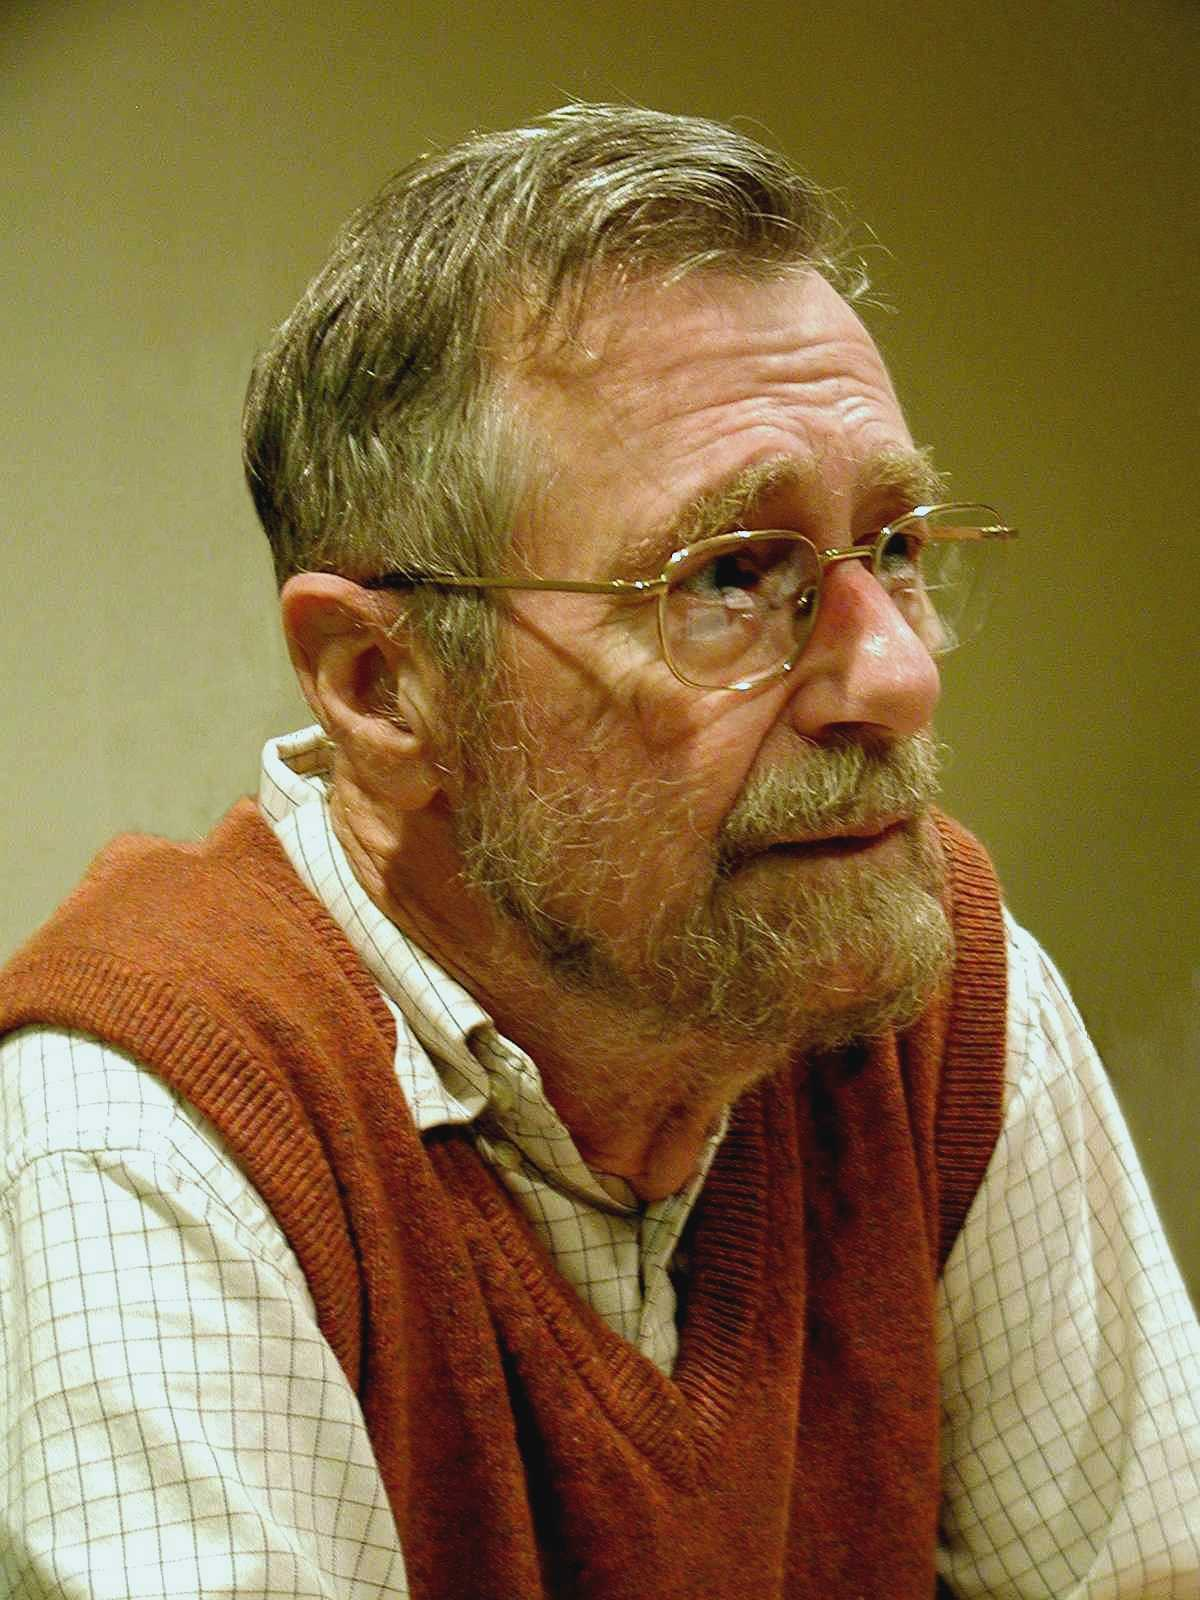
\includegraphics[height=1.15in]{images/dijkstra.jpg}\par
\medskip
{\small\itshape ``programming is as hard or as easy as proving''\par}
\smallskip
{\small Edsger W. Dijkstra\par}
{\scriptsize\href{https://www.cs.utexas.edu/~EWD/transcriptions/EWD12xx/EWD1243a.html}{\emph{The next fifty years} (excerpt)}\par}
\smallskip
{\scriptsize Photo: \copyright\ 2002 Hamilton Richards;\\
\href{https://www.cs.utexas.edu/~EWD/}{E. W. Dijkstra Archive, UT Austin}.\par}
\end{minipage}\hfill
\begin{minipage}[t]{0.46\textwidth}
\centering
\vspace{0pt}
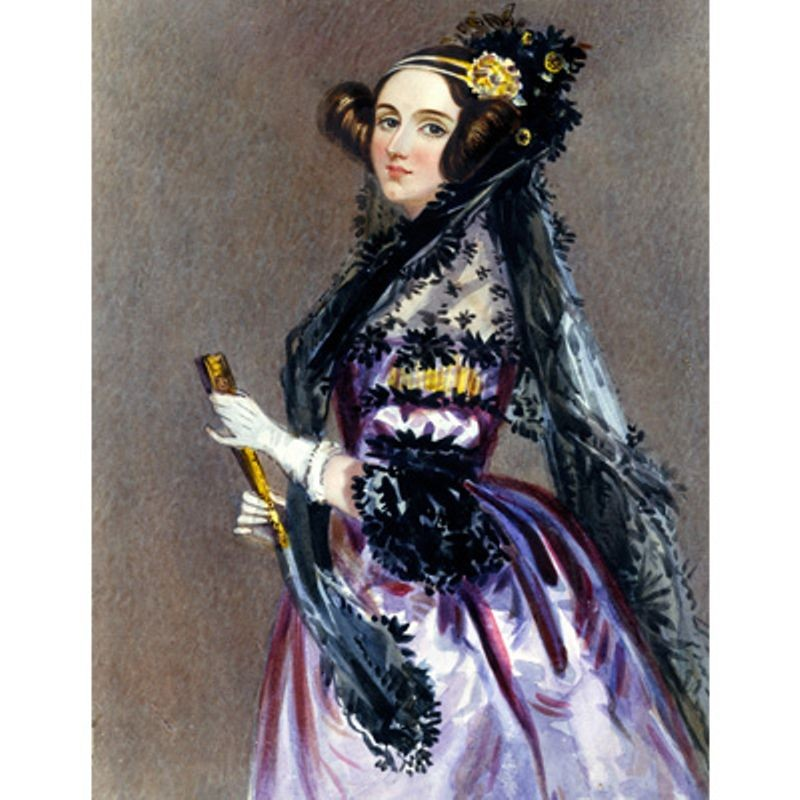
\includegraphics[height=1.15in]{images/lovelace.jpg}\par
\medskip
{\small\itshape ``The Analytical Engine weaves algebraic patterns just as the
Jacquard loom weaves flowers and leaves.''\par}
\smallskip
{\small Ada Lovelace, 1843\par}
{\scriptsize\href{https://www.computerhistory.org/babbage/adalovelace/}{As reproduced by the Computer History Museum}\par}
\smallskip
{\scriptsize Portrait, c. 1838: Science Museum;\\
via the Computer History Museum.\par}
\end{minipage}
\end{center}
\medskip

In the chapter on proofs, induction allowed us to establish infinitely many
claims using a base case and an inductive step. A closely related idea lets us
\emph{compute}: give the answer for a base case, and describe how to obtain a
new answer from answers to smaller problems. We have already done this when
we defined addition using the successor function. We now make that idea into
a model of computation.

\section{Why do we need a model of computation?}

An algorithm is a finite, unambiguous description of a procedure for obtaining
an answer from an input. For an algorithm that solves a problem on a stated
domain, the procedure must terminate and give the right answer on every input
in that domain. A description such as ``find the answer'' is not enough: we
must say what operations are available and how to combine them.

A model of computation supplies these rules. It separates the mathematical
procedure from the machine, programming language, or representation used to
carry it out. It also makes three different questions precise: what answer
is required, whether a procedure computes that answer, and how much work the
procedure takes. Two procedures can compute the same function with very
different amounts of work.

Our starting point is a function $f:\N\rightarrow\N$, where, as earlier,
$\N=\{0,1,2,\ldots\}$. An input is a natural number and a terminating
computation produces a natural number. We freely use functions of several
arguments, such as $\operatorname{add}:\N^2\rightarrow\N$. Using several arguments makes the notation easier to read. Pairs can be encoded as
single natural numbers; for example,
\[
\langle a,b\rangle=\frac{(a+b)(a+b+1)}{2}+b.
\]
This lists pairs by successive diagonals of $\N^2$. Its encoding and decoding
are effective finite procedures. Repeating the construction encodes tuples.
Finite strings, lists, and other finite data can likewise be represented by
natural numbers. This explains why numerical functions are a useful starting
point even when the eventual application concerns words or pictures.\footnote{
Ada Lovelace met Charles Babbage in 1833, when she was seventeen, and saw
him demonstrate a working section of his calculating engine. In her 1843
notes she went beyond arithmetic to envisage operations on other kinds of
symbols, even the composition of music. See the
\href{https://www.computerhistory.org/babbage/adalovelace/}{Computer History
Museum's account}.}

\section{Functions defined by induction}

Recall the successor function $S(n)=n+1$. We may start with zero, successor,
and functions that select an argument, and build new functions by
\emph{composition} and \emph{recursion}. Composition means using the output
of one function as the input of another: $h(n)=g(f(n))$.
A basic recursion scheme is
\[
f(\mathbf{x},m)=\begin{cases}
g(\mathbf{x}),&\text{if }m=0,\\
h(\mathbf{x},n,f(\mathbf{x},n)),&\text{otherwise}.
\end{cases}
\]
Here $\mathbf{x}$ denotes a tuple of additional arguments, and $g$ and $h$
are functions already constructed. In the otherwise branch, $n$ denotes
the unique predecessor of $m$, so $m=S(n)$; this branch is used only when
$m>0$. The recursive call decreases the last argument by one. These rules
determine a unique value on every input, provided the computations of $g$
and $h$ always finish on the inputs used.
This scheme is called \emph{primitive recursion}.

\subsection{Addition and multiplication}

Write $\operatorname{pred}(b)$ for the predecessor of a positive $b$, so
$\operatorname{pred}(S(n))=n$. It is used only in the nonzero branch.
To compute $a+b$, begin with $a+0=a$. If we can compute $a+n$, applying
successor gives $a+S(n)$. This proof pattern gives the algorithm
\[
\operatorname{add}(a,b)=\begin{cases}
a,&\text{if }b=0,\\
S(\operatorname{add}(a,\operatorname{pred}(b))),&\text{otherwise}.
\end{cases}
\]
\textbf{Correctness, by induction on $b$.}
\emph{Basis:} $\operatorname{add}(a,0)=a=a+0$ for every $a$.
\emph{Induction hypothesis:} for an arbitrary integer $n\geq0$ and every $a\in\N$,
$\operatorname{add}(a,n)=a+n$.
\emph{Inductive step:}
\[
\operatorname{add}(a,S(n))=S(\operatorname{add}(a,n))
=S(a+n)=a+S(n).
\]
The call decreases $b$ to its predecessor, so it also terminates.

For multiplication, the base product is zero. If we can compute $an$, one
more addition of $a$ gives $aS(n)$. Thus
\[
\operatorname{mul}(a,b)=\begin{cases}
0,&\text{if }b=0,\\
\operatorname{add}(\operatorname{mul}(a,\operatorname{pred}(b)),a),&\text{otherwise}.
\end{cases}
\]
\textbf{Correctness, by induction on $b$.}
\emph{Basis:} $\operatorname{mul}(a,0)=0=a\cdot0$.
\emph{Induction hypothesis:} for an arbitrary integer $n\geq0$,
$\operatorname{mul}(a,n)=an$ for every $a\in\N$.
\emph{Inductive step:} using the already established correctness of addition,
\[
\operatorname{mul}(a,S(n))
=\operatorname{add}(\operatorname{mul}(a,n),a)=an+a=aS(n).
\]
Again, the second argument decreases to zero. For example,
$\operatorname{mul}(4,3)$ computes $4+4+4$ through three additions to an
initial zero.

\paragraph{A notational simplification.}
From here onwards, we write $n+1$ instead of $S(n)$, and $n-1$ for the
predecessor when $n>0$. We also use ordinary addition and multiplication
symbols for the functions just constructed. These symbols abbreviate the computations we have just defined.

\subsection{Conditions, specifications, and algorithms}

Our specification language also includes \emph{if--then--else}. For example,
\[
K(x)=\begin{cases}
u(x),&\text{if }C(x),\\
v(x),&\text{otherwise}.
\end{cases}
\]
First evaluate the condition $C(x)$. If it is true, compute $u(x)$;
otherwise compute $v(x)$. Only the selected branch is evaluated. With more
than two cases, test the conditions in order and use the first that holds;
``otherwise'' covers the remaining inputs. For this to be an algorithm,
the test itself must have a definite computational procedure. The curly
braces alone do not make a mathematical specification executable.

For example, consider the following specification:
\[
\operatorname{sqrt}(n)=\begin{cases}
m,&\text{if some }m\in\N\text{ satisfies }m^2=n,\\
0,&\text{otherwise}.
\end{cases}
\]
The natural-number root, when it exists, is unique. This is a valid
specification: return the exact root for a perfect square and zero otherwise.
It also returns zero for $n=0$; zero is therefore not a distinct failure code.
But the first condition neither says how to find $m$ nor how to establish
that none exists. This description states the required answer without yet
providing a method of computing it.

A procedure can start with a candidate $m=0$ and test successive candidates:
\[
R(n,m)=\begin{cases}
m,&\text{if }m^2=n,\\
0,&\text{if }m^2>n,\\
R(n,m+1),&\text{otherwise}.
\end{cases}
\]
Evaluate $R(n,0)$. Each test is computable using multiplication and comparison.
Candidates smaller than $m$ have already been checked; once $m^2>n$, no
larger candidate can succeed. The search stops no later than $m=n+1$.
Thus it returns exactly the value specified above. For example,
$R(9,0)=R(9,1)=R(9,2)=R(9,3)=3$, whereas the search for $8$ stops at
$m=3$ and returns zero. The distinction is between a condition describing
an answer and instructions that actually find it.

We read our algorithmic equations as evaluation rules from left to right.
An equation such as $f(n)=f(n)$, by itself, gives no procedure for finding a
value. Neither a familiar function name nor mathematically valid notation
supplies the missing computational steps.

\paragraph{An algorithm can be read from a proof.}
The examples suggest a method of construction. Rather than guess a sequence
of steps, start with what is to be computed. Find a base case that can
be solved directly. Then assume that a smaller instance can be solved, and
show how its answer gives the answer to the current instance. The algorithm
is a \emph{computational rendering of this inductive proof}: the base case
becomes a stopping rule, the induction hypothesis becomes a recursive call,
and the inductive step becomes the computation using its result. Finding a
useful induction may require ingenuity, but the proof guides the construction.
\footnote{Dijkstra once illustrated the limits of exhaustive testing with
his university's multiplication hardware: at the quoted speed, trying every
possible pair of inputs would take roughly 30,000 years. His point was that
understanding why a procedure works can cover cases that we will never have
time to test individually. See
\href{https://www.cs.utexas.edu/~EWD/transcriptions/EWD03xx/EWD303.html}{EWD303,
``On the reliability of programs''}.}

A recursive call need not decrease an argument by exactly one. It may
decrease some other natural-number measure. The Well-Ordering Principle
rules out an infinite descent; induction on that measure proves correctness.
In the examples below, we make both the measure and the proof explicit.

\subsection{Quotient and remainder}
\label{sec:alg-division}

For $b>0$, the division theorem gives $a=bq+r$, with $0\leq r<b$.
We use \emph{induction on the quotient $q$} to construct the algorithms.
When $q=0$, $a<b$, so the quotient is zero and the remainder is $a$.
If $a=b(q+1)+r$, subtracting $b$ leaves $bq+r$: solve this smaller-quotient
problem, add one to its quotient, and keep its remainder. This gives
\[
\operatorname{div}(a,b)=\begin{cases}
0,&\text{if }a<b,\\
\operatorname{div}(a-b,b)+1,&\text{otherwise},
\end{cases}
\]
\[
\operatorname{mod}(a,b)=\begin{cases}
a,&\text{if }a<b,\\
\operatorname{mod}(a-b,b),&\text{otherwise}.
\end{cases}
\]
Subtraction and comparison are the natural-number operations introduced
earlier. Here $a-b$ is used only when $a\geq b$.

\textbf{Correctness, by induction on $q$.}
The precise claim is: for every $q\geq0$, every $b>0$, and every
$0\leq r<b$,
\[
\operatorname{div}(bq+r,b)=q,\qquad
\operatorname{mod}(bq+r,b)=r.
\]
\emph{Basis:} when $q=0$, the first argument is $r<b$, so the two base
branches return $0$ and $r$.
\emph{Induction hypothesis:} for an arbitrary integer $q\geq0$, both claims
hold for all $b>0$ and $0\leq r<b$.
\emph{Inductive step:} for $a=b(q+1)+r$, we have $a\geq b$ and $a-b=bq+r$.
Consequently,
\[
\begin{aligned}
\operatorname{div}(a,b)&=\operatorname{div}(bq+r,b)+1=q+1,\\
\operatorname{mod}(a,b)&=\operatorname{mod}(bq+r,b)=r.
\end{aligned}
\]
Each call reduces the quotient by one, so after $q$ calls the base case is
reached. The algorithm need not \emph{know} $q$ in advance: $q$ is the
measure used in its proof, and $a<b$ detects the stopping case.
For example,
\[
\begin{aligned}
\operatorname{div}(17,5)&=\operatorname{div}(12,5)+1
=(\operatorname{div}(7,5)+1)+1=3,\\
\operatorname{mod}(17,5)&=\operatorname{mod}(12,5)
=\operatorname{mod}(7,5)=\operatorname{mod}(2,5)=2.
\end{aligned}
\]
Division by zero is excluded from the domain.

\subsection{Powers and factorials}
\label{sec:alg-powers-factorials}

For $x,n\in\N$, the identities $x^0=1$ and $x^n=x^{n-1}x$ suggest
\[
\operatorname{pow}(x,n)=\begin{cases}
1,&\text{if }n=0,\\
\operatorname{pow}(x,n-1)\cdot x,&\text{otherwise}.
\end{cases}
\]
\textbf{Correctness, by induction on $n$.}
\emph{Basis:} $\operatorname{pow}(x,0)=1=x^0$.
\emph{Induction hypothesis:} for an arbitrary integer $k\geq0$,
$\operatorname{pow}(x,k)=x^k$ for every $x\in\N$.
\emph{Inductive step:}
$\operatorname{pow}(x,k+1)=\operatorname{pow}(x,k)x=x^kx=x^{k+1}$.
We adopt $0^0=1$ in this discrete definition, consistent with the empty
product. The exponent decreases to zero.

Similarly, $0!=1$ and $n!=n(n-1)!$ give
\[
\operatorname{fact}(n)=\begin{cases}
1,&\text{if }n=0,\\
n\cdot\operatorname{fact}(n-1),&\text{otherwise}.
\end{cases}
\]
\textbf{Correctness, by induction on $n$.}
\emph{Basis:} $\operatorname{fact}(0)=1=0!$.
\emph{Induction hypothesis:} for an arbitrary integer $k\geq0$,
$\operatorname{fact}(k)=k!$.
\emph{Inductive step:}
\[
\operatorname{fact}(k+1)=(k+1)\operatorname{fact}(k)=(k+1)k!=(k+1)!.
\]
The argument decreases to zero, proving termination. In each example, the
same induction both suggests the algorithm and establishes its correctness.

\subsection{Unfolding recursion: work that waits}
\label{sec:alg-deferred}

Let us follow the factorial algorithm exactly, at the level where
multiplication is available. Each recursive call leaves a multiplication
waiting for its answer:
\[
\begin{aligned}
\operatorname{fact}(5)
 &=5\cdot\operatorname{fact}(4)\\
 &=5\cdot(4\cdot\operatorname{fact}(3))\\
 &=5\cdot(4\cdot(3\cdot\operatorname{fact}(2)))\\
 &=5\cdot(4\cdot(3\cdot(2\cdot\operatorname{fact}(1))))\\
 &=5\cdot(4\cdot(3\cdot(2\cdot(1\cdot\operatorname{fact}(0)))))\\
 &=5\cdot(4\cdot(3\cdot(2\cdot(1\cdot1))))\\
 &=5\cdot(4\cdot(3\cdot(2\cdot1)))\\
 &=5\cdot(4\cdot(3\cdot2))\\
 &=5\cdot(4\cdot6)\\
 &=5\cdot24\\
 &=120.
\end{aligned}
\]
The expression first grows as the calls descend to zero. No multiplication
can yet be completed under these evaluation rules: the inner answer is not
available. After the base value $1$ is obtained, the expression shrinks as
the pending multiplications are performed. These are \emph{deferred
computations}. A direct evaluator remembers the unfinished calls in a
\emph{stack}.

Contrast this with computing the successive products $1,5,20,60,120,120$
as we count down from $5$ to $0$. Here every multiplication can be completed
immediately, and its result carried forward. In
Section~\ref{sec:alg-iteration} we will derive the tail-recursive algorithm
for this second process and trace the same input. Both function definitions
are recursive; only the first process accumulates deferred multiplications.

\subsection{Summing the values of a function}
\label{sec:alg-sum}

Suppose a procedure for computing $f(i)\in\N$ is already available and
finishes for every argument used. We want to compute
$\sum_{i=a}^{b}f(i)$ for $a,b\in\N$, taking an empty sum ($a>b$) as zero.
The empty interval is the base case. For a nonempty interval, the first term
plus the sum of the remaining terms gives the required answer:
\[
\operatorname{Sum}_f(a,b)=\begin{cases}
0,&\text{if }a>b,\\
f(a)+\operatorname{Sum}_f(a+1,b),&\text{otherwise}.
\end{cases}
\]
The subscript $f$ means that we use a fixed, already available function;
choosing another $f$ gives another summation procedure. For $f(i)=i^2$,
\[
\operatorname{Sum}_f(2,4)=4+(9+(16+0))=29.
\]
The additions are deferred until the recursive answers are available.

\textbf{Correctness, by induction on the number $\ell$ of terms.}
Here $\ell=0$ if $a>b$, and $\ell=b-a+1$ otherwise.
\emph{Basis:} an empty interval returns $0$, the empty sum.
\emph{Induction hypothesis:} for an arbitrary integer $k\geq0$, the
procedure returns the correct sum for \emph{every} interval of $k$ terms.
\emph{Inductive step:} an interval $[a,b]$ of $k+1$ terms has $k$ terms
remaining in $[a+1,b]$. Therefore
\[
\operatorname{Sum}_f(a,b)
=f(a)+\operatorname{Sum}_f(a+1,b)
=f(a)+\sum_{i=a+1}^{b}f(i)=\sum_{i=a}^{b}f(i).
\]
Each call removes one term, so the computation terminates. Notice that the
first argument increases: it is the \emph{number of remaining terms} that
decreases. Taking $f(i)=i$, $i^2$, or $1$ gives sums of integers, sums of
squares, or a count of terms using the same proof and algorithm.

\section{How much work? Complexity and Big O}

Correctness does not tell us whether a computation is practical.
\emph{Time complexity} counts work as the input grows; \emph{space
complexity} measures the storage needed. We begin by counting the main
operations: additions in summation, multiplications in factorial and powers,
and remainder computations in Euclid's algorithm.\footnote{These counts use
whole-number operations as units of work. They need not equal counts of
successor operations or individual bit operations. For example, a remainder
computed by repeated subtraction may require many elementary steps. A more
detailed analysis would expand the operations being counted.}\footnote{A
number's value and the length of its representation are different measures.
In binary, $n\geq1$ has $L=\lfloor\log_2 n\rfloor+1$ bits. A procedure
using $n$ steps can therefore take order $2^L$ steps in the input length.
Large-number arithmetic also costs more than small-number arithmetic.
We set these questions of bit complexity aside in this first discussion.}

\subsection{Recurrences count the work}

A \emph{time-complexity recurrence} expresses the work on an input in terms
of the work of its recursive calls, plus the work done outside those calls.
It has a base case, just like the algorithm. This is an important tool for
estimating steps: identify the calls, count the extra work, then unfold the
recurrence or bound its solution by induction. Count every recursive call;
two calls to the same smaller problem are still two computations unless
the result is explicitly computed once and reused.

For factorial, let $T(n)$ count multiplications. Reading the definition gives
\[
T(n)=\begin{cases}
0,&\text{if }n=0,\\
1+T(n-1),&\text{otherwise}.
\end{cases}
\]
Unfolding gives $T(n)=1+T(n-1)=2+T(n-2)=\cdots=n+T(0)=n$.
There are also $n+1$ factorial calls, and at most $n$ pending multiplications.
This measures the work of this algorithm, not a lower bound for every
possible factorial algorithm.

For summation, counting one addition per term gives
\[
A(\ell)=\begin{cases}
0,&\text{if }\ell=0,\\
A(\ell-1)+1,&\text{otherwise},
\end{cases}
\qquad\text{so }A(\ell)=\ell.
\]
There are also $\ell$ evaluations of $f$.\footnote{If evaluating $f(i)$
costs $C_f(i)$ steps, the full count includes $\sum_{i=a}^{b}C_f(i)$ as
well as additions and bookkeeping. Our addition count isolates the work
of the summation procedure itself.}

For successor-based addition, exactly $b$ successor operations are performed,
so the work grows linearly with $b$. Multiplication makes $b$ additions,
each applying successor $a$ times, for a total of $ab$ successor operations.
These simple counts already distinguish linear growth from growth in the
product of two inputs.\footnote{Including tests and call bookkeeping adds
work proportional to the number of calls. Under a constant cost for each
such step, addition is bounded by a constant times $b+1$, and multiplication
by a constant times $ab+b+1$. The extra terms account for zero inputs too.}

\begin{definition}[Big O]
For nonnegative functions $T$ and $g$, we write $T(n)=O(g(n))$ if there are
constants $C>0$ and $n_0$ such that
\[
T(n)\leq Cg(n)\qquad\text{for all }n\geq n_0.
\]
\end{definition}
Thus $3n+7=O(n)$: for $n\geq1$, $3n+7\leq10n$. Constant factors and
lower-order terms do not affect this upper bound. Big O need not be tight:
$3n+7$ is also $O(n^2)$, although the linear bound tells us more. Typical
orders of growth are $O(1)$, $O(\log n)$, $O(n)$, $O(n\log n)$, $O(n^2)$, and $O(2^n)$.
Big O itself does not mean ``worst case''; we first choose whether $T$
measures worst-case, average, or some particular execution cost.

\subsection{Seeing the difference in growth rates}

Figure~\ref{fig:alg-growth} plots representative functions for the five
orders of growth. The curves are $\log_2 n$, $n$, $n\log_2 n$, $n^2$,
and $2^n$ themselves: Big O denotes a class of upper bounds, not one
particular curve. Constant factors are taken as one for comparison.

\begin{figure}[htbp]
\centering
\begin{tikzpicture}
\begin{axis}[
width=0.88\textwidth,height=5.2cm,
xmin=2,xmax=32,ymin=0,ymax=1100,
xlabel={$n$},ylabel={Work $f(n)$},
title={Ordinary vertical scale},
xtick={2,8,16,24,32},ytick={0,250,500,750,1000},
grid=major,grid style={gray!20},
tick label style={font=\small},label style={font=\small},
legend style={font=\small,at={(0.5,-0.27)},anchor=north,draw=none},
legend columns=5]
\addplot[blue,thick,domain=2:32,samples=100] {ln(x)/ln(2)};
\addlegendentry{$\log_2 n$}
\addplot[black,thick,dashed,domain=2:32] {x};
\addlegendentry{$n$}
\addplot[teal,thick,dashdotted,domain=2:32,samples=100] {x*ln(x)/ln(2)};
\addlegendentry{$n\log_2 n$}
\addplot[orange!85!black,thick,densely dotted,domain=2:32,samples=100] {x*x};
\addlegendentry{$n^2$}
\addplot[red!75!black,thick,domain=2:11,samples=100] {2^x};
\addlegendentry{$2^n$}
\end{axis}
\end{tikzpicture}

\medskip
\begin{tikzpicture}
\begin{semilogyaxis}[
width=0.88\textwidth,height=5.2cm,
xmin=2,xmax=100,ymin=1,ymax=1e31,
xlabel={$n$},ylabel={Work $f(n)$ (log scale)},
title={Each vertical interval multiplies work by $10^5$},
xtick={2,20,40,60,80,100},
ytick={1,1e5,1e10,1e15,1e20,1e25,1e30},
grid=major,grid style={gray!20},
tick label style={font=\small},label style={font=\small}]
\addplot[blue,thick,domain=2:100,samples=100] {ln(x)/ln(2)};
\addplot[black,thick,dashed,domain=2:100] {x};
\addplot[teal,thick,dashdotted,domain=2:100,samples=100] {x*ln(x)/ln(2)};
\addplot[orange!85!black,thick,densely dotted,domain=2:100,samples=100] {x*x};
\addplot[red!75!black,thick,domain=2:100,samples=100] {2^x};
\end{semilogyaxis}
\end{tikzpicture}
\caption{Five growth rates on two scales; the same styles identify curves
in both panels. In the upper panel, $2^n$ leaves the displayed range just
after $n=10$. The logarithmic scale below keeps it visible up to $n=100$;
its straight appearance there represents exponential growth.}
\label{fig:alg-growth}
\end{figure}

Doubling $n$ adds one to $\log_2 n$, doubles $n$, changes $n\log_2 n$
by a factor $2(1+1/\log_2 n)$, and quadruples $n^2$. For $2^n$, doubling
$n$ \emph{squares the amount of work}. Even increasing $n$ by just one
doubles it. These statements concern the displayed functions, not arbitrary
algorithms known only to satisfy the corresponding Big O upper bounds.

\paragraph{How bad is exponential growth?}
Suppose an algorithm actually performs $2^n$ steps, and imagine a machine
performing a billion ($10^9$) of those steps each second. Then:
\begin{center}
\begin{tabular}{r r l}
\hline
$n$ & Steps $2^n$ (approximately) & Time (approximately)\\
\hline
10 & $1.02\times10^3$ & $1.02$ microseconds\\
30 & $1.07\times10^9$ & $1.07$ seconds\\
50 & $1.13\times10^{15}$ & $13$ days\\
100 & $1.27\times10^{30}$ & $4.02\times10^{13}$ years\\
\hline
\end{tabular}
\end{center}
At $n=100$, the other four representative counts are only about $6.64$,
$100$, $664$, and $10{,}000$. A machine a thousand times faster buys the
exponential algorithm only $\log_2 1000\approx10$ additional units of input
in the same time budget. Better hardware changes a constant factor; a
better algorithm may change the growth rate. Exponential algorithms can
still be useful for small inputs, but scale very poorly. An $O(2^n)$ upper
bound alone does not establish exponential behaviour; the example assumes
an actual $2^n$ step count.

\subsection{A faster way to compute powers}
\label{sec:alg-fast-power}

The power algorithm removes one factor at a time. Can we make a bigger
reduction? If we know $x^k$, one squaring gives $x^{2k}$; one further
multiplication by $x$ gives $x^{2k+1}$. Define the helper
\[
\operatorname{sqr}(y)=y\cdot y.
\]
Then use the parity of the exponent to choose the appropriate rule:
\[
E(x,n)=\begin{cases}
1,&\text{if }n=0,\\
\operatorname{sqr}(E(x,\operatorname{div}(n,2))),&\text{if }n\text{ is even},\\
x\cdot\operatorname{sqr}(E(x,\operatorname{div}(n,2))),&\text{otherwise}.
\end{cases}
\]
Only one branch is used. In that branch the argument of $\operatorname{sqr}$
is evaluated once; the helper then multiplies the resulting number by itself.
Thus there is just one recursive call at each level.

\textbf{Correctness, by strong induction on the exponent $n$.}
\emph{Basis:} $E(x,0)=1=x^0$ for every $x\in\N$.
\emph{Induction hypothesis:} for an arbitrary integer $n\geq1$, assume
$E(x,j)=x^j$ for every integer $0\leq j<n$ and every $x\in\N$.
\emph{Inductive step:} put $k=\operatorname{div}(n,2)$, so $0\leq k<n$.
If $n=2k$, the algorithm returns $(x^k)^2=x^n$ by the hypothesis.
If $n=2k+1$, it returns $x(x^k)^2=x^n$. In both cases the recursive
exponent is smaller, so the computation also terminates.

\paragraph{Deriving the logarithmic bound.}
Let $M(n)$ be the number of multiplications made by this fast-power algorithm.
Its exact recurrence is
\[
M(n)=\begin{cases}
0,&\text{if }n=0,\\
M(\lfloor n/2\rfloor)+1,&\text{if }n>0\text{ is even},\\
M(\lfloor n/2\rfloor)+2,&\text{otherwise}.
\end{cases}
\]
There is one recursive call; an even exponent adds one multiplication,
and an odd exponent adds two. For $n\geq1$, after
$L=\lfloor\log_2 n\rfloor+1$ halvings the exponent is zero. Hence
\[
L\leq M(n)\leq2L,
\qquad M(n)=O(\log{n}).
\]
Equivalently, unfold the upper-bound recurrence
$M(n)\leq M(\lfloor n/2\rfloor)+2$ for $L$ levels.
For $n=16$, the exponents are $16,8,4,2,1,0$, and the count is
$1+1+1+1+2=6$, compared with $16$ multiplications for ordinary power.

The helper $\operatorname{sqr}$ matters. Replacing it by two separate calls
$E(x,\operatorname{div}(n,2))\cdot E(x,\operatorname{div}(n,2))$ would repeat
the smaller computation. For even $n$, the new multiplication count would
satisfy $D(n)=2D(n/2)+1$. Unfolding this recurrence for $n=2^k$ gives
$D(2^k)=3\cdot2^k-1$, since $D(1)=2$: the count is now linear in $n$.
Halving the problem helps only if we avoid doing the same work twice.
\footnote{The logarithmic bound counts multiplications. It treats the
halving and parity tests as auxiliary operations; implementing division by
repeated subtraction would add further work. The sizes of the multiplied
numbers matter in a bit-operation analysis.}

\subsection{Euclid's algorithm: correctness and efficiency}
\label{sec:alg-euclid}

For $a,b\in\N$ not both zero, the greatest common divisor is the largest
positive integer dividing both. Euclid's algorithm gives a particularly
clear example of a proof guiding an efficient computation.\footnote{In
\href{https://mathcs.clarku.edu/~djoyce/elements/bookVII/propVII2.html}{Book VII,
Proposition 2 of the \emph{Elements}}, Euclid describes the reduction by
continually subtracting the smaller number from the larger. Computing a
remainder packages several such subtractions into one step. The notation
has changed, but the common-divisor argument is the same.} Its key is the
following claim.

\textbf{Claim.} If $a=bq+r$, $b>0$, and $0\leq r<b$, then
$\gcd(a,b)=\gcd(b,r)$.
\emph{Proof:} let $d=\gcd(a,b)$. Since $d$ divides both $a$ and $b$, it
divides $r=a-bq$, so it is a common divisor of $b,r$. Conversely, any
positive common divisor $c$ of $b,r$ divides $bq+r=a$, so it is a common
divisor of $a,b$ and hence $c\leq d$. Thus $d$ is the greatest common
divisor of $b,r$. This includes $r=0$.

The claim reduces the second argument from $b$ to $r<b$. Assuming we can
solve all such smaller cases, we obtain the algorithm
\[
G(a,b)=\begin{cases}
a,&\text{if }b=0,\\
G(b,\operatorname{mod}(a,b)),&\text{otherwise}.
\end{cases}
\]
\textbf{Correctness, by strong induction on $b$.}
We prove $G(a,b)=\gcd(a,b)$ for every $b\geq0$ and \emph{every} $a>0$.
\emph{Basis:} $G(a,0)=a=\gcd(a,0)$.
\emph{Induction hypothesis:} for an arbitrary integer $k\geq0$,
assume that for all integers $0\leq j\leq k$ and all $u>0$,
$G(u,j)=\gcd(u,j)$.
\emph{Inductive step:} let $b=k+1$ and $r=\operatorname{mod}(a,b)$.
Since $0\leq r<b$ and $b>0$,
\[
G(a,b)=G(b,r)=\gcd(b,r)=\gcd(a,b).
\]
The middle equality uses the induction hypothesis, and the last uses the
claim. Quantifying over \emph{every} first argument is essential: the
recursive call changes it from $a$ to $b$. The decreasing second argument
also proves termination.

For completeness, if $a=0<b$, the algorithm returns $G(b,0)=b$, as required.
We may set $G(0,0)=0$ by convention to obtain a numerical function defined on every pair;
this does not assert that zero has a greatest positive divisor.
For example,
\[
G(48,18)=G(18,12)=G(12,6)=G(6,0)=6.
\]
The following chapter on primes and gcd develops the number-theoretic
consequences further.

\paragraph{Why logarithmically many steps?}

Let $C(a,b)$ count remainder computations. Directly from the algorithm,
\[
C(a,b)=\begin{cases}
0,&\text{if }b=0,\\
1+C(b,\operatorname{mod}(a,b)),&\text{otherwise}.
\end{cases}
\]
Merely observing that the second argument decreases proves termination,
but gives only a crude linear bound. We need to show that it shrinks quickly.
Put $r=\operatorname{mod}(a,b)$, so $0\leq r<b$. If $r=0$, we stop after
one step. If $0<r\leq b/2$, the new second argument is already at most half
of $b$. Otherwise $b/2<r<b$, so the next remainder is
\[
\operatorname{mod}(b,r)=b-r<b/2,
\]
because $b$ contains exactly one copy of $r$. Thus within at most two
remainder steps, either the computation stops or its second argument at
least halves.

After at most $2\lceil\log_2 b\rceil$ steps, a starting $b\geq1$ has
therefore either reached zero or become at most $1$; one further step then
finishes. Hence
\[
C(a,b)\leq2\lceil\log_2 b\rceil+1\quad(b\geq1).
\]
This shows that the algorithm requires $O(\log b)$  steps. It requires no assumption that $a\geq b$.\footnote{The
bound counts remainder computations. It does not count the subtractions
or bit operations used to implement each remainder.}

\section{Iteration through tail recursion}
\label{sec:alg-iteration}

Return to factorial. To avoid deferred multiplications, let $p$ record the
product already computed and $k$ count the factors still to be processed.
We want $p=n!$ when $k=0$. A useful relation to maintain throughout is
\[
0\leq k\leq n,\qquad p\cdot k!=n!.
\]
Initially this holds with $(k,p)=(n,1)$. If $k>0$, replacing $(k,p)$ by
$(k-1,pk)$ preserves the relation, since $(pk)(k-1)!=pk!$.
This reasoning \emph{derives} the algorithm
\[
F(k,p)=\begin{cases}
p,&\text{if }k=0,\\
F(k-1,p\cdot k),&\text{otherwise}.
\end{cases}
\]
To compute $n!$, evaluate $F(n,1)$. Its evaluation for $n=5$ is
\[
\begin{aligned}
F(5,1)&=F(4,5)\\
      &=F(3,20)\\
      &=F(2,60)\\
      &=F(1,120)\\
      &=F(0,120)\\
      &=120.
\end{aligned}
\]
At each transition the multiplication is carried out \emph{before} the next
call. Compare the two factorial computations:
\begin{center}
\begin{tabular}{p{0.43\textwidth} p{0.43\textwidth}}
\hline
\textbf{Deferred computation} & \textbf{Direct accumulation}\\
\hline
$5\cdot\operatorname{fact}(4)$ waits for the inner answer.
& $F(5,1)\longrightarrow F(4,5)$ carries a completed product.\\
Pending multiplications accumulate, then are performed on return.
& Completed products are carried forward in $p$.\\
The evaluator remembers unfinished work.
& The current state $(k,p)$ contains all the information needed.\\
\hline
\end{tabular}
\end{center}

In $F$, nothing remains to be done with the result of the recursive call.
Such a call is in \emph{tail position}; a function whose recursive calls
all have this form is \emph{tail recursive}. A recursively written function
can therefore generate an \emph{iterative process}: repeatedly replace a
current state by a next state, without accumulating unfinished calls.
In general,
\[
I(s)=\begin{cases}
\operatorname{answer}(s),&\text{if }\operatorname{stop}(s),\\
I(\operatorname{next}(s)),&\text{otherwise}.
\end{cases}
\]
The state $s$ may be a tuple of natural numbers. Tail recursion alone does
not guarantee termination: we must still show that a stopping state is reached.

\subsection{Invariants are induction over state changes}
\label{sec:alg-invariants}

An \emph{invariant} is a statement about the current state, possibly also
referring to the fixed original input, that holds initially and is preserved
by every transition. The values of the state variables change; the truth of
the statement does not. To establish correctness using an invariant, check:
\begin{enumerate}
\item \emph{Initialisation:} the initial state satisfies it.
\item \emph{Preservation:} if it holds before a nonterminal step, it holds
      after that step.
\item \emph{Conclusion:} the invariant together with the stopping condition
      implies that the returned answer is the required one.
\end{enumerate}
This is induction on the number $t$ of transitions. Initialisation proves
the claim for $t=0$. For an arbitrary integer $t\geq0$, assume the
invariant holds after $t$ transitions. Preservation proves it after the
next transition, if one is made. A separate termination argument shows
that a stopping state is eventually reached.

For $F(n,1)$, the invariant we designed was $0\leq k\leq n$ and $pk!=n!$.
\emph{Initialisation:} $1\cdot n!=n!$.
\emph{Preservation:} $(pk)(k-1)!=pk!=n!$ and $0\leq k-1\leq n$ when $k>0$.
\emph{Conclusion:} at $k=0$, $p\cdot0!=p=n!$.
\emph{Termination:} $k$ decreases by one and cannot decrease below zero.
This shows how an invariant can guide the design, not merely check an
algorithm after it has been written.

The same result can be proved by induction on $k$, the number of factors
remaining. The claim is: \emph{for every $k,p\in\N$, $F(k,p)=p\cdot k!$}.
\emph{Basis:} $F(0,p)=p=p\cdot0!$.
\emph{Induction hypothesis:} for an arbitrary integer $k\geq0$,
$F(k,u)=u\cdot k!$ for \emph{every} accumulator $u\in\N$.
\emph{Inductive step:}
\[
F(k+1,p)=F(k,p(k+1))=p(k+1)k!=p(k+1)!.
\]
Taking $p=1$ gives the desired factorial. The hypothesis must cover every
accumulator, since its value changes in the recursive call.

\subsection{Further examples of iterative processes}
\label{sec:alg-iterative-examples}

For addition, begin with $(a,b)=(a_0,b_0)$ and preserve $a+b=a_0+b_0$:
\[
A(a,b)=\begin{cases}
a,&\text{if }b=0,\\
A(a+1,b-1),&\text{otherwise}.
\end{cases}
\]
The initial equality is immediate. Each step preserves it because
$(a+1)+(b-1)=a+b$. At termination $b=0$, so the returned $a$ equals
$a_0+b_0$; termination follows from decreasing $b$.
For example, $A(4,3)=A(5,2)=A(6,1)=A(7,0)=7$.

Multiplication and powers use an accumulator in the same way:
\[
M(a,k,p)=\begin{cases}
p,&\text{if }k=0,\\
M(a,k-1,p+a),&\text{otherwise},
\end{cases}
\]
\[
P(x,k,p)=\begin{cases}
p,&\text{if }k=0,\\
P(x,k-1,p\cdot x),&\text{otherwise}.
\end{cases}
\]
For $ab$, start with $M(a,b,0)$ and maintain $p+ak=ab$.
The initial equality is $0+ab=ab$, a step preserves it since
$(p+a)+a(k-1)=p+ak$, and $k=0$ implies $p=ab$.
For $x^n$, start with $P(x,n,1)$ and maintain $px^k=x^n$.
It holds initially, is preserved by $(px)x^{k-1}=px^k$ for $k>0$, and
implies $p=x^n$ at $k=0$. Both counters decrease to zero. Include
$0\leq k\leq b$ or $0\leq k\leq n$, respectively, in the invariants.

Euclid's $G$ is already tail recursive. For an initial pair $(a_0,b_0)$
not both zero, its invariant is
\[
a,b\in\N,\quad a+b>0,\quad \gcd(a,b)=\gcd(a_0,b_0).
\]
It holds initially. The common-divisor claim proves preservation under
$(a,b)\mapsto(b,\operatorname{mod}(a,b))$, and $b>0$ ensures the new pair
is not $(0,0)$. When $b=0$, the invariant says the returned $a$ is the
original gcd. The second argument decreases, proving termination. Thus the
inductive proof and the invariant express the same mathematical reason for
correctness in two forms.

\subsection{Summation as iteration}
\label{sec:alg-sum-iteration}

For the same fixed function $f$ as in Section~\ref{sec:alg-sum}, use $c$ as
the next index and $s$ as the sum already accumulated:
\[
J_f(c,b,s)=\begin{cases}
s,&\text{if }c>b,\\
J_f(c+1,b,s+f(c)),&\text{otherwise}.
\end{cases}
\]
To compute $\sum_{i=a}^{b}f(i)$, start with $J_f(a,b,0)$.
For $f(i)=i^2$ the computation is
\[
J_f(2,4,0)=J_f(3,4,4)=J_f(4,4,13)=J_f(5,4,29)=29.
\]
Every addition is completed before the next call, in contrast with the
nested additions in $\operatorname{Sum}_f(2,4)$.

If $a>b$, the initial call immediately returns the empty sum. Otherwise
an invariant for the initial interval $[a,b]$ is
\[
a\leq c\leq b+1,\qquad s=\sum_{i=a}^{c-1}f(i).
\]
Equivalently, the accumulated sum plus the remaining sum equals the target:
\[
s+\sum_{i=c}^{b}f(i)=\sum_{i=a}^{b}f(i).
\]
\emph{Initialisation:} $c=a$ and $s=0$, the sum over an empty prefix.
\emph{Preservation:} when $c\leq b$, adding $f(c)$ extends the prefix by
one term, and replacing $c$ by $c+1$ identifies the next unprocessed term.
\emph{Conclusion:} stopping gives $c=b+1$, so $s=\sum_{i=a}^{b}f(i)$.
\emph{Termination:} $b-c+1$, the number of remaining terms, decreases to zero.
Again, the invariant tells us what to initialise, how to update the state,
and when to return the answer.

Both versions evaluate $f$ and add once per term: their addition count is
$\ell=b-a+1$ for $a\leq b$. Tail recursion removes the chain of deferred
additions without changing that count.\footnote{The work and storage
needed inside $f$ itself are additional in both versions.}

\paragraph{What does tail recursion save?}
The direct factorial computation leaves $n$ multiplications waiting for
answers. The accumulator version still performs $n$ multiplications, but
carries only the current pair $(k,p)$. It replaces a growing record of
unfinished work by a fixed number of state variables.\footnote{An evaluator
must reuse tail calls as state transitions to obtain this storage saving;
one that retains every call frame may still build a stack. A fixed number
of variables is not a fixed number of bits: the accumulator eventually
holds $n!$. Storage and work inside arithmetic helpers must also be counted
in a more detailed analysis.} This is a change in how the work is organised,
not a reduction in the number of multiplications.

\section{How far does this model reach?}

\subsection{Why these rules are a reasonable model}

Imagine carrying out a calculation with pencil and paper, following explicit
instructions without inventing new steps. At any moment there is a finite
record: the input, intermediate numbers, and the instruction to perform next.
One step reads part of this record, performs a specified elementary operation,
and produces a new record. It may choose what to do next by a test. A long
computation repeats such steps until its stopping condition is met.

Our model expresses these ingredients directly. Numbers encode finite data;
composition connects one calculation to the next; if--then--else makes a
choice using a computable test; and recursion describes repetition. As we
saw with iteration, a tuple can hold the entire current state. Including the
current instruction in that state also permits different operations at
different stages. The amount of data and the number of steps need not have
a fixed universal bound: each completed computation uses only finitely much.
These observations explain the model's plausibility without reference to
any particular machine or programming language.

There is one limitation to address. Primitive recursion repeats a
construction a number of times controlled by a supplied natural number.
It guarantees termination when its component computations terminate, but
there are effective procedures that cannot be expressed using only those
rules. To describe computation in general, we must also allow continuing
until a computable test succeeds, without requiring a previously supplied
bound on how many trials to make.

\subsection{Bounded search and unbounded search}

A \emph{bounded search}, also called \emph{bounded minimisation}, tests
$y=0,1,\ldots,B$ and returns the first successful candidate, or reports that
none in that range works. The bound $B$ may depend on the input; it need not
be a constant. If the test always finishes, the search always finishes.
For square roots, such a bound is available: no natural-number root of $n$
can exceed $n$ when $n\geq1$, and $n=0$ is immediate. Our earlier procedure
uses the sharper stopping test $m^2>n$.

But failure up to $B$ means only ``no solution yet'', unless we can prove
that no later candidate could succeed. Imagine running a given procedure
for successively larger limits: first $0$ steps, then $1$, then $2$, and so
on, each time checking whether it has finished. Every bounded trial is a
finite task. Failure to finish within $B$ steps does not show that the
procedure will never finish.
Requiring a suitable bound to be computed first would impose an extra task
on every procedure. The ability to take the next step does not require such
a bound to be known in advance.

Bounded search can already be expressed by primitive recursion, provided
its bound and tests can: count through the permitted candidates and remember
the first success. Adding this kind of search therefore gives no new
computational power. Some terminating procedures lie beyond these rules,
though proving this is beyond our scope. Allowing a more powerful procedure
to compute the bound would simply move the difficulty into that procedure.

In \emph{unbounded search}, we keep trying the next candidate until the test
succeeds. For a previously constructed numerical procedure $g$, write
\[
H(\mathbf{x},y)=\begin{cases}
y,&\text{if }g(\mathbf{x},y)=0,\\
H(\mathbf{x},y+1),&\text{otherwise}.
\end{cases}
\]
Start with $H(\mathbf{x},0)$. Each test must finish before proceeding to the
next candidate. If no test succeeds, or a required test never finishes, this
computation produces no answer. ``Unbounded'' means no advance cutoff, not
that a successful search performs infinitely many steps. If the first
successful candidate is $k$ and all preceding tests finish, only $k+1$
candidates are tested.

\subsection{What completeness means}

Informally, a \emph{total function} assigns an answer to every input in its
stated domain. A \emph{partial function} may leave some inputs without an
answer. In our computational setting, this latter possibility describes a
procedure that runs forever on some inputs. All the arithmetic algorithms
above finish on their stated domains; permitting unbounded search means
that our language can also describe computations that fail to finish.
For example, searching only for $y^2=n$, with no overshoot test, never
finishes on a nonsquare. The bounded square-root algorithm shows that this
failure belongs to that particular search procedure, not to the problem.

Starting with the elementary numerical functions and closing under
composition, primitive recursion, and unbounded search gives the standard
\emph{partial recursive} model. Computable conditionals can be expressed
within it. Its rules themselves are mechanical, and the state-and-step
view above explains why it is reasonable to regard them as sufficient for
any effective calculation on finite data. This is an argument for the
model's adequacy, not a proof that every imaginable mathematical function
has an algorithm.

The same idea of effective calculation can be approached in different ways.
Alan Turing described a machine that follows elementary rules for reading,
writing, and moving among symbols. Alonzo Church approached computation
through functions and rules for applying them. Their starting points look
quite different, yet both models compute exactly the same numerical
functions as the recursive model we have described. This equivalence is a
mathematical theorem.

\begin{figure}[ht]
\centerline{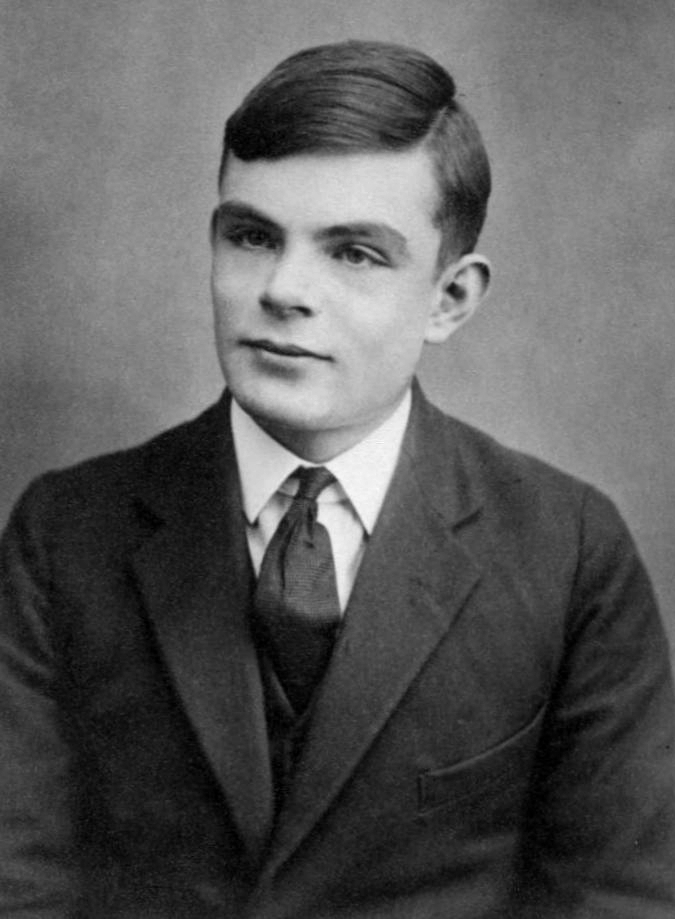
\includegraphics[width=1.0in]{images/turing.jpg}}
\caption*{\small ``A function is said to be `effectively calculable' if its
values can be found by some purely mechanical process.'' -- Alan Turing,
\href{https://doi.org/10.1112/plms/s2-45.1.161}{\emph{Systems of Logic Based
on Ordinals}} (1939), p.~166.}
\end{figure}

\begin{figure}[ht]
\centerline{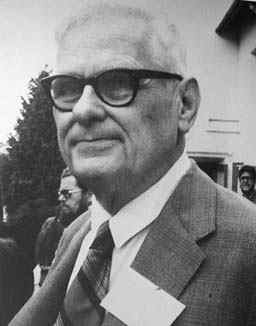
\includegraphics[width=1.0in]{images/church.jpg}}
\caption*{\small ``a function of positive integers shall be called
effectively calculable if it is recursive'' -- Alonzo Church,
\href{https://phil415.pbworks.com/f/Church.pdf}{\emph{An Unsolvable Problem
of Elementary Number Theory}} (1936), p.~346, footnote~3 (excerpt).}
\end{figure}

The agreement of these independently developed models gives us confidence
that they capture the informal idea of calculation by explicit, mechanical
rules. The assertion that they encompass \emph{every effective mechanical
procedure} is the \emph{Church--Turing thesis}. Unlike the equivalence of
the formal models, this assertion is not a mathematical theorem: it connects
a precise mathematical definition with an informal idea. In Church's
quotation, ``recursive'' includes the possibility of unbounded search;
primitive recursion alone would not suffice. We need no knowledge of the
other models to use ours. Its scope concerns what can be computed, not
whether every procedure we write terminates or gives the intended answer.




\section*{Problems}
\begin{enumerate}
\item Unfold $\operatorname{add}(2,4)$ and $\operatorname{fact}(5)$.
Mark the operations that are deferred. Trace the corresponding tail-recursive
computations and identify their states.
\item State the induction hypothesis for division and remainder using the
quotient $q$. Explain why using $q$ in the proof does not require knowing
it before running the algorithm.
\item Trace quotient and remainder for $(23,4)$. Define a tail-recursive
function that computes both together, using a remainder candidate and a
quotient accumulator. State and prove its invariant.
\item Trace $G(105,252)$. Explain why an initial assumption $a\geq b$ is
unnecessary, and why the second argument is a suitable termination measure.
\item Prove that $5n^2+3n+8=O(n^2)$. Explain why an $O(n^2)$ upper bound
alone does not establish that an algorithm needs quadratic time.
\item Compare the number of multiplications for $3^{16}$ using
$\operatorname{pow}$ and $E$, following the definitions exactly. Explain
what happens if $\operatorname{sqr}$ is replaced by two independently
evaluated recursive calls.
\item Explain how the invariant for $F(k,p)$ determines its next state. Describe which value must be used
in the multiplication if the two components of its state are updated one
at a time.
\item Under the hypothetical rate of $10^9$ steps per second, estimate the
time for $2^{60}$ steps. How much does a thousandfold speed-up increase the
input size possible in a fixed time? Compare with an algorithm taking $n^2$
steps.
\item For $f(i)=2i+1$, unfold $\operatorname{Sum}_f(1,3)$ and trace
$J_f(1,3,0)$. Check the invariant at each state, and state the addition-count
recurrence. What changes if one evaluation of $f(i)$ costs $i$ steps?
\item Prove the upper bound for fast power by induction using its recurrence.
Explain why counting one recursive call instead of two is decisive.
\item In Euclid's algorithm, show that two consecutive positive remainders
cannot both exceed half the earlier second argument. Use this to derive
a logarithmic bound without assuming anything about Fibonacci numbers.
\item Explain why ``no successful candidate at most $B$'' does not usually
mean ``no successful candidate exists''. What extra fact makes a bounded
search sufficient in the square-root example?
\item Explain why the unbounded search for a square root may fail to halt.
Modify it to return a special failure code when no natural-number square root
exists, and explain why the modified search always terminates.
\item Define recursive and tail-recursive algorithms for
$\prod_{i=a}^{b}f(i)$, with an empty product equal to $1$. Prove the recursive
version correct by induction on the number of factors. Give an invariant
for the iterative version.
\item Let $B(0)=1$ and $B(n)=B(n-1)+B(n-1)$ for $n>0$. Show by induction
on $n$ that $B(n)=2^n$. If the two recursive calls are evaluated separately,
derive the recurrence for the number of additions and solve it. Rewrite the
algorithm to use only $n$ additions.
\item The Fibonacci numbers are $F_0=0$, $F_1=1$, and
$F_{n+2}=F_{n+1}+F_n$. Design an iterative algorithm that starts with
$(i,u,v)=(0,0,1)$ and maintains $u=F_i$, $v=F_{i+1}$. State its stopping
condition, prove correctness, and count its additions.
\item Evaluate $G(34,21)$ and $G(55,34)$. Compare the successive remainders
with the Fibonacci numbers. Explain why each reduction is small compared
with the case in which the smaller input divides the larger exactly.
\item Construct a tail-recursive fast-power algorithm using a state $(b,k,p)$
with invariant $p b^k=x^n$. Start with $(b,k,p)=(x,n,1)$.
What state change works when $k$ is even? What works when it is odd?
Prove that the algorithm terminates and uses logarithmically many
multiplications. State what happens when $n=0$.
\item To count how many values among $f(a),\ldots,f(b)$ are even, define a
recursive algorithm using an if--then--else test. Prove it correct by induction
on the number of terms. Then derive an iterative version and its invariant.
\item Suppose an algorithm has a correct invariant but its state never
changes. Must it return the right answer? Give an example and explain
precisely what an invariant proves and what a termination argument adds.
\end{enumerate}

% Includable chapter; uses amsmath, amssymb, algorithm, algpseudocode,
% tikz, hyperref, caption. These are already present in the main notes.
\chapter{Changing state, preserving truth:  the Imperative model of computation}
\label{chap:imperative}
\vspace{-0.5in}
%\noindent{\LARGE\itshape The Imperative model of computation}\par\bigskip
\begin{center}
\begin{minipage}[t]{0.48\textwidth}
\centering\vspace{0pt}
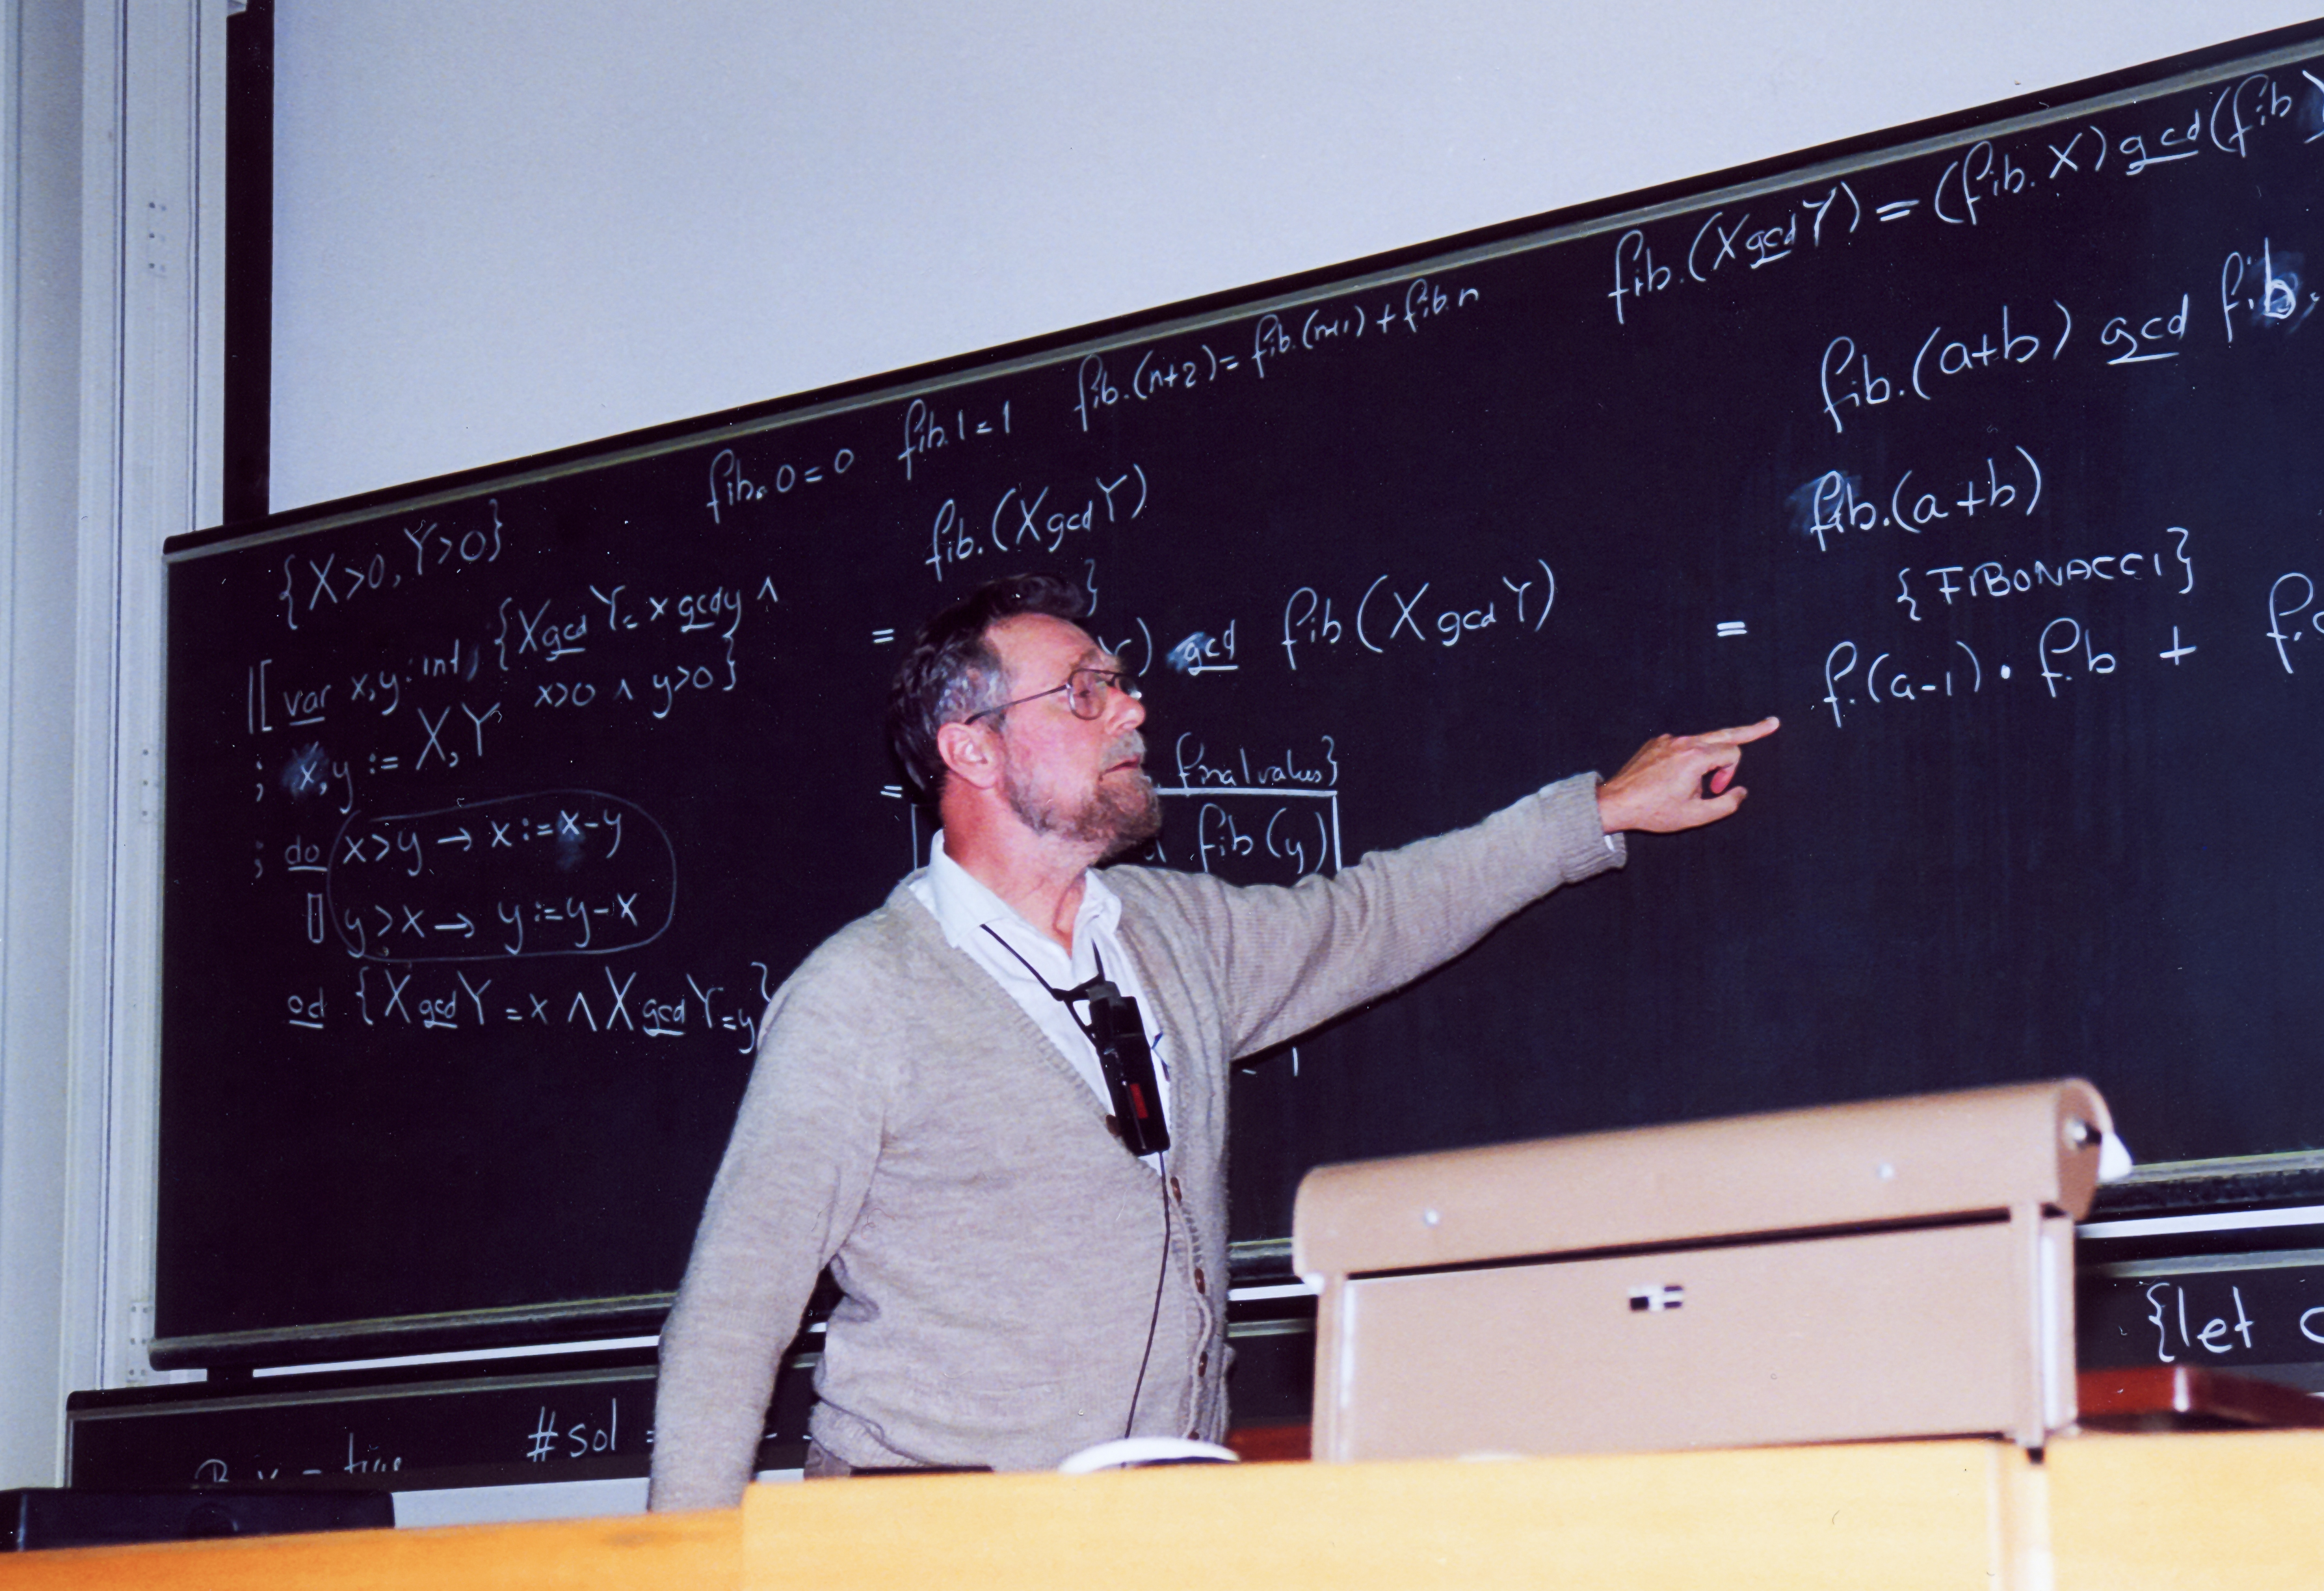
\includegraphics[height=1.12in]{images/dijkstra-1994.jpg}
\captionof*{figure}{\small ``one designs the correctness proof and derives
the program from that proof.''\\
---Edsger W. Dijkstra, \href{https://www.cs.utexas.edu/~EWD/transcriptions/EWD10xx/EWD1073.html}{EWD~1073} (excerpt).}
{\scriptsize ETH Zurich, 1994. Photo: Andreas F. Borchert,
\href{https://creativecommons.org/licenses/by-sa/4.0/}{CC BY-SA 4.0}.}
\end{minipage}\hfill
\begin{minipage}[t]{0.48\textwidth}
\centering\vspace{0pt}
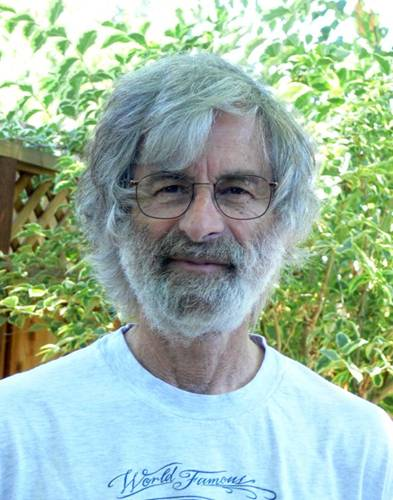
\includegraphics[height=1.12in]{images/lamport.jpg}
\captionof*{figure}{\small ``Invariants play an important role in understanding
algorithms and programs.''\\
---Leslie Lamport, \href{https://lamport.azurewebsites.net/pubs/state-machine.pdf}{\emph{Computation and State Machines}}, Section~5.1.1.}
{\scriptsize \href{https://awards.acm.org/award_winners/_1205376.cfm}{2013 Turing Award}. Photo courtesy Leslie Lamport.}
\end{minipage}
\end{center}

In Chapter~\ref{chap:algorithms}, an iterative computation passed its current state
to the next call. For factorial, the state $(k,p)$ was replaced by
$(k-1,pk)$ until $k=0$. The invariant $p\cdot k!=n!$ explained why the
answer survived each change. We now describe the same process by storing
$k$ and $p$ and giving instructions that change their contents.

This is the \emph{imperative model}: a computation is a sequence of
commands that transform a stored state. We will keep asking two questions.
What changes when a command is performed? What remains true despite that
change? The first describes the computation; the second helps us design it
and prove that it works.

Our procedures use mathematical notation and ordinary instructions, in the
style of the ruler-and-compass constructions. They do not depend on a
particular programming language. The available actions will be stated in
each setting: storing a number, exchanging two entries, placing a tile, or
moving a disk. A more detailed implementation would explain how to carry
out these actions on a particular machine.

\section{Variables become places to store values}

In the equation $y=x+1$, the letters denote mathematical values. In a
functional call $F(4,1)$, the parameters receive those values for that call;
a later call $F(3,4)$ has a new set of parameter values. Neither changes
the meaning of the earlier call.

An imperative variable has a different role. Think of it as the name of a
storage location, or a labelled box. The name stays the same while the
value in the box may change. A \emph{state} is a snapshot of the contents
of the boxes. To describe the complete progress of a computation we also
need to know which instruction comes next.

We write $x\leftarrow e$ for \emph{assignment}: evaluate the expression
$e$ using the current contents of the variables, and then store the result
in $x$, replacing its previous contents. Other locations retain their
contents. Thus $x\leftarrow x+1$ is a perfectly sensible command. If $x$
contains $4$, it will contain $5$ afterwards. The equation $x=x+1$, by
contrast, is false for every integer $x$. We reserve $=$ for equality.

\begin{figure}[ht]
\centering
\begin{tikzpicture}
\node at (0,0.65) {before}; \node at (5,0.65) {after};
\draw (-0.65,-0.35) rectangle (0.65,0.35);\node at (0,0) {$4$};\node at (0,-0.65) {$x$};
\draw (4.35,-0.35) rectangle (5.65,0.35);\node at (5,0) {$5$};\node at (5,-0.65) {$x$};
\draw[->,thick] (1,0)--(4,0) node[midway,above] {$x\leftarrow x+1$};
\end{tikzpicture}
\caption{The location retains its name; assignment replaces its contents.}
\end{figure}

Start with $x=4$ and perform $y\leftarrow x$ followed by $x\leftarrow x+1$.
The final state is $x=5$, $y=4$. The first command copied a value; it did
not make $y$ follow all later changes to $x$. In our model, differently
named scalar variables denote separate locations. Every variable must be
assigned a value before an instruction reads it.\footnote{Real languages
also offer ways for several names to refer to the same storage. We do not
need that additional complication here. Our mathematical integers have no
fixed upper limit; a machine implementation must provide suitable storage.}

In the procedure displays, comments beginning with \texttt{\# PRE},
\texttt{\# INV}, and \texttt{\# POST} state the required initial condition,
loop invariant, and promised final condition. A \texttt{\# BOUND} comment
states a decreasing bound function for termination, defined below. A \texttt{\# ASSERT} comment
records an intermediate fact. They are mathematical statements, not
instructions. A straight-line procedure has intermediate assertions rather
than a loop invariant.

\subsection{Order matters: exchanging two values}

Suppose $x$ and $y$ initially contain $A$ and $B$. Here $A$ and $B$ are
fixed mathematical names for the original values, not locations that the
procedure changes. We want to finish with $x=B$ and $y=A$.
The commands $x\leftarrow y$ followed by $y\leftarrow x$ do not achieve
this: the first destroys the old value of $x$, and both boxes finish with
$B$. We must save the value before overwriting it.

\begin{algorithm}[H]
\begin{algorithmic}[1]
\Procedure{Exchange}{$x,y$}
\Statex \texttt{\# PRE:} $x=A$, $y=B$; $A,B$ are fixed original values.
\State Store the current contents of $x$ in a temporary location $t$.
\Statex \texttt{\# ASSERT:} $t=A$, $x=A$, $y=B$.
\State $x\leftarrow y$
\Statex \texttt{\# ASSERT:} $t=A$, $x=B$, $y=B$.
\State $y\leftarrow t$
\Statex \texttt{\# POST:} $x=B$, $y=A$.
\EndProcedure
\end{algorithmic}
\caption{Exchange the contents of two specified locations.}
\end{algorithm}

\[
\begin{array}{c|ccc}
 &x&y&t\\\hline
\text{initially}&A&B&\text{unused}\\
\text{after the first command}&A&B&A\\
\text{after the second command}&B&B&A\\
\text{after the third command}&B&A&A
\end{array}
\]
A command reads the state left by the preceding command. Translating a
simultaneous state transition into separate assignments therefore requires
care: save any old value that will still be needed.

\section{Commands, decisions, and repetition}

We use three ways to organise commands.
\begin{enumerate}
\item \emph{Sequence}: perform commands in the stated order.
\item \emph{Selection}: \textbf{if} a condition is true, perform one block
of commands; \textbf{otherwise}, perform the other. Only the chosen block
is performed.
\item \emph{Repetition}: \textbf{while} a condition is true, perform a
block of commands, then test the condition again.
\end{enumerate}
The condition of a while loop is checked \emph{before} each repetition,
so the block may be performed zero times. Indentation identifies the
commands belonging to a block. A call to a named procedure performs its
commands and then resumes the calling procedure.

For example, to store the larger of $a$ and $b$ in $m$, use
\begin{algorithmic}[1]
\Statex \texttt{\# PRE:} $a=A$, $b=B$ are comparable values.
\If{$a\geq b$}
\State $m\leftarrow a$
\Else
\State $m\leftarrow b$
\EndIf
\Statex \texttt{\# POST:} $m=\max(A,B)$, $a=A$, $b=B$.
\end{algorithmic}
The test asks a question about the current state; it does not change either
value. An assignment changes the state. Keeping these roles separate is
essential.

\subsection{What a procedure promises}

Before designing a procedure, state its \emph{precondition}: what must be
true when it begins. State its \emph{postcondition}: what it must make
true when it finishes. For Exchange these are, respectively,
\[
x=A\ \text{and}\ y=B,\qquad x=B\ \text{and}\ y=A.
\]
An \emph{assertion} is a mathematical statement about a state at a specified
point in a procedure. It describes what we claim, rather than instructing
the machine to make the claim true. Our proof must justify it.

Correctness has two parts: the procedure must finish, and its final state
must satisfy the postcondition whenever its initial state satisfies the
precondition. A rule that would give the right answer \emph{if} it finished
is not enough to solve the problem on every permitted input.

\section{A loop invariant is an induction hypothesis}

The tail-recursive factorial construction in Section~\ref{sec:alg-iteration}, with its invariant proved in Section~\ref{sec:alg-invariants}, gives the transition
$(k,p)\mapsto(k-1,pk)$. We now store the two components and update them
with assignments. The same invariant guides these updates.

Start with the desired loop postcondition: $k=0$ and $p=n!$.
To generalise it, allow unfinished work, represented by $k!$, so that
$p\cdot k!=n!$. At $k=0$ this reduces to the required answer.
At each test of the loop condition, we therefore claim
\[
I:\qquad 0\leq k\leq n\quad\text{and}\quad p\cdot k!=n!.
\]
This is a \emph{loop invariant}. Its truth is preserved from one test of
the condition to the next, even though the values in it change.
It need not hold between every pair of commands inside the loop.


To obtain $p=n!$ at the end, let $k!$ represent the work still to do.
The invariant suggests starting with $k=n$ and $p=1$, and stopping at
$k=0$. When $k>0$, decreasing $k$ by one must be balanced by multiplying
$p$ by the old $k$, because $(pk)(k-1)!=pk!$. Thus the multiplication must
precede the decrement. We obtain the following commands from that reasoning.

\begin{algorithm}[H]
\begin{algorithmic}[1]
\Procedure{Factorial}{$n$}
\Statex \texttt{\# PRE:} $n\in\mathbb N$ is fixed.
\State $k\leftarrow n$
\State $p\leftarrow1$
\Statex \texttt{\# INV:} $k,p\in\mathbb N$, $0\leq k\leq n$, $p\cdot k!=n!$.
\Statex \texttt{\# BOUND:} $k$.
\While{$k>0$}
\State $p\leftarrow p\cdot k$
\State $k\leftarrow k-1$
\EndWhile
\Statex \texttt{\# POST:} $k=0$ and $p=n!$; $n$ is unchanged.
\State \Return $p$
\EndProcedure
\end{algorithmic}
\caption{Factorial by successive changes of state.}
\end{algorithm}

\paragraph{Initialisation.}
Before the first test, $k=n$ and $p=1$, so $I$ holds.

\paragraph{Preservation.}
Suppose $I$ holds at a test for which $k>0$. Call the values at that point
$K$ and $P$. The two commands produce $p=PK$ and $k=K-1$. Since $K\geq1$,
\[
p\cdot k!=(PK)(K-1)!=P K!=n!.
\]
The bounds on $k$ persist too. This proves preservation for one execution
of the \emph{whole} loop body.

\paragraph{Exit.}
When the condition becomes false, $k\leq0$. Together with the invariant
this gives $k=0$, and hence $p=n!$.

\paragraph{Termination.}
A \emph{bound function} assigns a nonnegative integer to each state
at a loop test. Whenever the body executes, its value must strictly
decrease from one test to the next. It therefore decreases monotonically
along the computation, and cannot decrease forever. If its initial value
is $B$, there can be at most $B$ repetitions, provided each execution of
the body itself finishes. The bound need not decrease by exactly one,
and the loop may stop before it reaches zero.

For factorial the bound function is $k$: it starts at $n$ and decreases
by one on every repetition. A bound function is also called a
\emph{loop variant}. An invariant tells us what remains true; a bound
function establishes progress towards termination. Merely never increasing
is insufficient: a constant value would permit endless repetition.
Nor is strict decrease among nonnegative real numbers enough: the sequence
$1,1/2,1/4,\ldots$ never ends. Here we use nonnegative integers.

Where was induction used? We induct on the number $j$ of completed
repetitions. The invariant holds for $j=0$. For every integer $j\geq0$,
if it holds after $j$ repetitions and another repetition is performed,
preservation shows that it holds after $j+1$. Thus it holds at every
reached test, including the final one. This is the induction principle
applied to a computation's history.

For $n=4$, the states $(k,p)$ at successive tests are
\[
(4,1),\ (3,4),\ (2,12),\ (1,24),\ (0,24).
\]
They are the same states as in the tail-recursive version. The model of
description has changed; the invariant and the computation have not.

\subsection{From the postcondition to the invariant and the loop}

We first stated the factorial postcondition, then generalised it to an
invariant before writing commands. The invariant supplied
the initial state, the update, and the stopping condition. Reversing the
two assignments would multiply by the new $k$ and break that reasoning.
This order of development applies to the remaining examples too.
Begin with the final assertion, and generalise it to describe partial
progress: replace a completed range by a growing prefix, allow an
unfinished remainder, or retain a smaller equivalent problem. Keep the
conditions that protect data and preserve the meaning of the answer.
The invariant must be weak enough to hold initially and strong enough to
yield the postcondition at exit. This is a design method, not a mechanical
recipe for finding an invariant.
For a loop with invariant $I$ and condition $C$, prove:
\begin{enumerate}
\item The initialisation establishes $I$.
\item If $I$ and $C$ hold, the body re-establishes $I$.
\item $I$ together with the failure of $C$ implies the required answer.
\item A nonnegative integer bound function strictly decreases on every
execution of the body, and each execution finishes.
\end{enumerate}
The first three establish the answer on exit; the fourth establishes that
exit is reached. A loop that repeatedly leaves $k$ unchanged can preserve
$k\geq0$ forever. Preservation alone does not imply progress.

\section{Familiar computations, now with stored state}

\subsection{Summation: the processed part and the remaining part}

Recall the recursive sum in Section~\ref{sec:alg-sum} and its iterative
form in Section~\ref{sec:alg-sum-iteration}. We now implement that same
accumulation by assignments.

Let $f:\mathbb N\to\mathbb N$ be a function whose values can always be computed, and let $a,b\in\mathbb N$.
The loop postcondition is $k>b$ and $s=\sum_{i=a}^{b}f(i)$,
taking an empty sum to be zero. Generalise the completed upper endpoint
$b$ to $k-1$: only the terms before the moving index $k$ have been added.
The inputs and the rule for $f$ remain fixed throughout the procedure.
Choose a location $s$ for the sum so far and a location $k$ for the next
index to be processed. The invariant, including the empty-interval case, is
\[
a\leq k\leq\max(a,b+1),\qquad s=\sum_{i=a}^{k-1}f(i).
\]
The empty processed part suggests $k=a$, $s=0$. To extend it by one term,
add $f(k)$ before advancing $k$.

The same invariant can be written as
\[
s+\sum_{i=k}^{b}f(i)=\sum_{i=a}^{b}f(i).
\]
Work already done and work still to do together make the whole task.
This is a useful pattern for discovering invariants.

\begin{algorithm}[H]
\begin{algorithmic}[1]
\Procedure{Sum}{$f,a,b$}
\Statex \texttt{\# PRE:} $a,b\in\mathbb N$; $f:\mathbb N\to\mathbb N$ is computable; inputs fixed.
\State $s\leftarrow0$
\State $k\leftarrow a$
\Statex \texttt{\# INV:} $s\in\mathbb N$, $a\leq k\leq\max(a,b+1)$,
\Statex \texttt{\#} $s=\sum_{t=a}^{k-1}f(t)$; $f,a,b$ unchanged.
\Statex \texttt{\# BOUND:} $\max(0,b-k+1)$.
\While{$k\leq b$}
\State $s\leftarrow s+f(k)$
\State $k\leftarrow k+1$
\EndWhile
\Statex \texttt{\# POST:} $k>b$, $s=\sum_{t=a}^{b}f(t)$ (zero for an empty interval).
\State \Return $s$
\EndProcedure
\end{algorithmic}
\caption{Accumulate the sum of successive function values.}
\end{algorithm}

Initially the sum in the invariant is empty. If the old index is $K\leq b$,
then the updated values satisfy
\[
s_{\rm new}=\sum_{i=a}^{K-1}f(i)+f(K)=\sum_{i=a}^{K}f(i),
\qquad k_{\rm new}=K+1.
\]
Thus the invariant is preserved. Induction on the number of completed
repetitions, beginning at zero and with the step valid for every integer
$j\geq0$ for which the loop continues, proves it at every test. At exit, if $a\leq b$, then $k=b+1$, so the sum is the desired one.
The bound function $\max(0,b-k+1)$ decreases by one whenever the body
executes. Each evaluation of $f$ finishes by the precondition. If $a>b$,
the loop is skipped and returns zero, as required.

The procedure evaluates $f$ exactly $b-a+1$ times when $a\leq b$.
Its total time must also include the cost of those evaluations.

\subsection{Quotient and remainder together}

Section~\ref{sec:alg-division} constructed quotient and remainder by
repeated subtraction. Here we compute both together, retaining the same
relationship that justified the inductive step. For fixed $a\geq0$ and
$b>0$, the postcondition is $a=bq+r$, $q\geq0$, and $0\leq r<b$.
Generalise it by dropping the final restriction $r<b$: the remainder may
still contain whole copies of $b$. Maintain
\[
a=bq+r,\qquad q\geq0,\quad r\geq0.
\]
Here $q$ counts the copies of $b$ already removed, while $r$ is what remains.
The invariant suggests $q=0,r=a$ initially. If $r\geq b$, subtracting
$b$ from $r$ must be balanced by adding one to $q$. Stopping when $r<b$
then gives both the quotient and the required remainder bound. These
choices follow from the relationship we have decided to preserve.

\begin{algorithm}[H]
\begin{algorithmic}[1]
\Procedure{Divide}{$a,b$}
\Statex \texttt{\# PRE:} $a,b\in\mathbb N$ and $b>0$.
\State $q\leftarrow0$
\State $r\leftarrow a$
\Statex \texttt{\# INV:} $q,r\in\mathbb N$, $a=bq+r$; $a,b$ fixed.
\Statex \texttt{\# BOUND:} $r$.
\While{$r\geq b$}
\State $r\leftarrow r-b$
\State $q\leftarrow q+1$
\EndWhile
\Statex \texttt{\# POST:} $a=bq+r$, $q\geq0$, $0\leq r<b$; inputs unchanged.
\State \Return $(q,r)$
\EndProcedure
\end{algorithmic}
\caption{Each repetition removes one more copy of the divisor.}
\end{algorithm}

Initialisation is immediate. If $a=bQ+R$ and $R\geq b$, then
$a=b(Q+1)+(R-b)$, so the full body preserves the invariant and nonnegativity.
This is induction on the number of completed subtractions, which is the
quotient counter $q$: the base is $q=0$, and the step applies to every
integer $q\geq0$ for which another subtraction is made.
At exit $0\leq r<b$, giving precisely the quotient and remainder conditions.
The bound function is the nonnegative remainder $r$; it strictly decreases on every repetition.
For $(a,b)=(17,5)$, the states $(q,r)$ at tests are
$(0,17),(1,12),(2,7),(3,2)$.

\subsection{Euclid: preserving the answer while changing the problem}

Section~\ref{sec:alg-euclid} proved the common-divisor property, and
Section~\ref{sec:alg-iterative-examples} expressed it as an invariant.
The functional transition $(u,v)\mapsto(v,\operatorname{mod}(u,v))$
preserves the gcd. To realise it with assignments, compute the remainder
before overwriting $u$.

For fixed inputs $a,b\in\mathbb N$ not both zero, the loop postcondition
is $v=0$ and $u=\gcd(a,b)$. Since $\gcd(u,0)=u$ for $u>0$,
rewrite the answer as $\gcd(u,v)=\gcd(a,b)$ at $v=0$.
Generalise by allowing $v$ to be nonzero, while keeping the gcd fixed.
This gives the invariant
\[
u,v\in\mathbb N,\qquad u+v>0,\qquad \gcd(u,v)=\gcd(a,b).
\]
Initialising $(u,v)=(a,b)$ establishes it. The common-divisor property
suggests the update above, while the stopping condition $v=0$ makes the
invariant yield $u=\gcd(a,b)$. Temporary storage lets us implement that
update without losing an old value that is still needed.

\begin{algorithm}[H]
\begin{algorithmic}[1]
\Procedure{Euclid}{$a,b$}
\Statex \texttt{\# PRE:} $a,b\in\mathbb N$, not both zero.
\State $u\leftarrow a$
\State $v\leftarrow b$
\Statex \texttt{\# INV:} $u,v\in\mathbb N$, $u+v>0$, $\gcd(u,v)=\gcd(a,b)$; $a,b$ fixed.
\Statex \texttt{\# BOUND:} $v$.
\While{$v>0$}
\State $r\leftarrow\operatorname{mod}(u,v)$
\State $u\leftarrow v$
\State $v\leftarrow r$
\EndWhile
\Statex \texttt{\# POST:} $v=0$, $u=\gcd(a,b)$; inputs unchanged.
\State \Return $u$
\EndProcedure
\end{algorithmic}
\caption{Preserve the gcd, using temporary storage for the remainder.}
\end{algorithm}

The chosen invariant holds initially. The common-divisor argument from
Section~\ref{sec:alg-euclid} proves preservation for the complete body. Induction
on the number of completed repetitions proves it at every test, with base
zero and the preservation step for every reached iteration.
On exit $v=0$, so $u=\gcd(a,b)$. The new $v$ is smaller than the old
positive $v$. Thus $v$ is a bound function, proving termination. The logarithmic bound on the
number of remainder steps from Section~\ref{sec:alg-euclid} is unchanged
by this translation.

\section{Lists and a non-numerical invariant}

Suppose a list occupies indexed locations $L[1],\ldots,L[m]$. An entry
may contain a letter, a name, or another finite object. Reading $L[i]$
retrieves that entry; assigning to $L[i]$ replaces it. We can reverse the
list by exchanging its outermost entries and moving inwards.

Let $L_0$ be the fixed original list of length $m$. Write $L[a..b]$
for an indexed segment, empty if $a>b$, and write $\operatorname{rev}(S)$
for a sequence $S$ read backwards. These describe mathematical sequences;
no extra copies need be stored. Relax the final requirement
$L=\operatorname{rev}(L_0)$ by marking exactly which segments are finished.
At each loop test the invariant is
\[
\begin{gathered}
|L|=m,\quad 1\leq\ell\leq m+1,\quad 0\leq r\leq m,\\
\ell\leq r+1,\qquad \ell+r=m+1,\\
L[1..\ell-1]=\operatorname{rev}(L_0[r+1..m]),\\
L[\ell..r]=L_0[\ell..r],\\
L[r+1..m]=\operatorname{rev}(L_0[1..\ell-1]).
\end{gathered}
\]
Thus the current left end is the reversal of the corresponding original
right end; the current right end is the reversal of the original left end;
and the entire middle is still unchanged. The two finished ends are not
asserted to be reversals of \emph{each other}. Their relation is to the
original list, which need not be a palindrome.
\[
\underbrace{L[1..\ell-1]}_{\text{finished left end}}\quad
\underbrace{L[\ell..r]}_{\text{unchanged middle}}\quad
\underbrace{L[r+1..m]}_{\text{finished right end}}.
\]
Initialising $\ell=1,r=m$ makes both finished ends empty. While $\ell<r$,
the equality $\ell+r=m+1$ identifies two original entries that belong
in each other's final positions. Exchanging them and moving the boundaries
inwards extends both finished ends. When $\ell\geq r$, the middle is
empty or is the single central entry, whose original position is already
its final position. The invariant then implies that the whole list is
reversed. This gives the procedure below.

\begin{algorithm}[H]
\begin{algorithmic}[1]
\Procedure{Reverse}{$L,m$}
\Statex \texttt{\# PRE:} $L=L_0$, $|L_0|=m\geq0$; $m$ fixed.
\State $\ell\leftarrow1$
\State $r\leftarrow m$
\Statex \texttt{\# INV:} $|L|=m$, $1\leq\ell\leq m+1$, $0\leq r\leq m$,
\Statex \texttt{\#} $\ell\leq r+1$, $\ell+r=m+1$.
\Statex \texttt{\#} $L[1..\ell-1]=\operatorname{rev}(L_0[r+1..m])$.
\Statex \texttt{\#} $L[\ell..r]=L_0[\ell..r]$.
\Statex \texttt{\#} $L[r+1..m]=\operatorname{rev}(L_0[1..\ell-1])$.
\Statex \texttt{\# BOUND:} $\max(0,r-\ell+1)$.
\While{$\ell<r$}
\State Exchange the contents of locations $L[\ell]$ and $L[r]$.
\State $\ell\leftarrow\ell+1$
\State $r\leftarrow r-1$
\EndWhile
\Statex \texttt{\# POST:} $\ell\geq r$, $|L|=m$, $L=\operatorname{rev}(L_0)$.
\EndProcedure
\end{algorithmic}
\caption{Reverse a list by modifying its entries.}
\end{algorithm}

Initially the outside part is empty. If $\ell<r$, the two untouched
end entries belong in each other's positions because $r=m+1-\ell$.
Exchanging them and moving the boundaries preserves the claim. Induction
on the number of completed exchanges, with base zero and the step for each
integer $j\geq0$ at which another exchange is made, proves the invariant.

At exit there are either no unprocessed entries or just the middle entry,
which is already in its correct position. Thus the list is reversed.
The bound function $\max(0,r-\ell+1)$ decreases by two whenever the loop runs,
so it terminates after $\lfloor m/2\rfloor$ exchanges. For example,
\[
[\mathrm A,\mathrm B,\mathrm C,\mathrm D,\mathrm E]
\longrightarrow[\mathrm E,\mathrm B,\mathrm C,\mathrm D,\mathrm A]
\longrightarrow[\mathrm E,\mathrm D,\mathrm C,\mathrm B,\mathrm A].
\]
The output is a changed arrangement, and the invariant describes which
part of that arrangement is finished.

\section{Searching for an entry in a list}
\label{sec:imp-search}

Random access means that $L[i]$ gives direct access to the entry at index
$i$; it does not mean that the index is chosen by chance. We count an
entry access, assignment, or comparison as one operation.\footnote{This
is a model of indexed storage. Following links in a chain or comparing
long strings can have additional costs.}

We shall work on a segment $L[l..r]$ of a list of length $m$, where
$1\leq l\leq r+1\leq m+1$. It is empty when $l=r+1$.
The parameters $l,r,m,x$ remain
fixed. All index variables are integers. Assertions over empty segments
are true. In every procedure below the input assertions, loop invariants,
and output assertions are written as comments beginning with \texttt{\#}.
They describe the states to be established, not extra commands to execute.

\subsection{Sequential search}
\label{sec:imp-linear-search}

\paragraph{Specify the answer.}
Given an established segment and a target $x$, return its first matching
index, or $-1$ if there is no match. The list must remain unchanged.
Use a Boolean variable $found$ and an index $i$. The loop postcondition
is: 
\[
(found\ \text{and }\ (l\leq i\leq r\ \text{and }L[i]=x))\ \text{or } (\neg found\ \text{and } (L[t]\ne x\quad\text{for every }l\leq t<r+1)).
\]
Either $found$ is true and $L[i]$ is the first match, or $found$ is false and
$i=r+1$, which indicates that every entry of the segment differs from $x$.  Generalise the completed unsuccessful scan by allowing $i$ to
mark an unfinished position.

\paragraph{Relax the final assertion to obtain the invariant.}
Instead of claiming that the entire segment has been searched, describe
the part before $i$. At every loop test require the following invariant to hold
\[
\begin{gathered}
l\leq i\leq r+1,\\
(found\ \text{and }\ (l\leq i\leq r\ \text{and }L[i]=x))\ \text{or } (\neg found\ \text{and } (L[t]\ne x\quad\text{for every }l\leq t<i))
\end{gathered}
\]
The prefix before $i$ has been ruled out. If $found$ is true, the current
entry is a valid first match. If it is false, the current entry may still
need to be checked: false does not assert absence from the whole segment.
This distinction keeps the invariant true both before and after success.

\paragraph{Initialise, then preserve.}
Set $found$ to false and $i=l$. The ruled-out prefix is empty.
Continue while no match is recorded and $i\leq r$. If $L[i]=x$, set
$found$ to true and retain $i$ as the answer. Otherwise increase $i$:
the failed comparison allows this entry to join the ruled-out prefix.
At exit either a first match is recorded, or $i=r+1$ and the entire
segment has been ruled out. The commands follow from these assertions.

\begin{algorithm}[H]
\begin{algorithmic}[1]
\Procedure{SequentialSearch}{$L,l,r,x$}
\Statex \texttt{\# PRE:} $|L|=m$, $1\leq l\leq r+1\leq m+1$; $x$ is established.
\State $found\leftarrow\mathrm{false}$; $i\leftarrow l$
\Statex \texttt{\# INV:} $(found\ \text{and }\ (l\leq i\leq r\ \text{and }L[i]=x))\ \text{or } (\neg found\ \text{and } (L[t]\ne x\quad\text{for every }l\leq t<i))$,
\Statex \texttt{\#}  $l\leq i\leq r+1$
\Statex \texttt{\# BOUND:} $r-i+1$ if not $found$, otherwise $0$.
\While{$\neg found$ and $i\leq r$}
\If{$L[i]=x$}
\State $found\leftarrow\mathrm{true}$
\Else
\State $i\leftarrow i+1$
\EndIf
\EndWhile
\Statex \texttt{\# POST:} $(found\ \text{and }\ (l\leq i\leq r\ \text{and }L[i]=x))\ \text{or } (\neg found\ \text{and } (L[t]\ne x\quad\text{for every }l\leq t<r+1))$
\If{$found$}
\State \Return $i$
\Else
\State \Return $-1$
\EndIf
\EndProcedure
\end{algorithmic}
\caption{Search by extending a prefix known not to contain the target.}
\end{algorithm}

Induct on the number of completed iterations. Initialisation proves the
base case zero; the two cases just described preserve every clause for
any integer $t\geq0$ at which another iteration is made. On success the
loop stops; on failure $r-i+1$ decreases. Equivalently, use the bound function
$r-i+1$ when $found$ is false and zero otherwise. Each executed iteration
strictly decreases it. There are at most $r-l+1$ comparisons for a nonempty
segment, so the worst-case work is linear in its length.

\subsection{Binary search}
\label{sec:imp-binary-search}

\paragraph{}
Now consider that the given segment is sorted in nondecreasing order. Return any matching
index, or $-1$ if the target is absent, without changing the list. We can then construct a more efficient search algorithm.

This is also a search problem, and the loop postcondition is unchanged: 
\[
(found\ \text{and }\ (l\leq i\leq r\ \text{and }L[i]=x))\ \text{or } (\neg found\ \text{and } (L[t]\ne x\quad\text{for every }l\leq t \leq r)).
\]
 Since the list is sorted in the increasing order, 
a middle entry smaller than $x$ excludes itself and every entry to its
left; a larger entry excludes itself and every entry to its right.
We therefore relax the final assertion by keeping a candidate interval
$[left,right]$ inside the original segment.

\paragraph{The invariant.}
Let $mid = \operatorname{div}(left+right,2)$. Then, we can define the invariant condition by relaxing the postcondition as:
\[
\begin{gathered}
(found\ \text{and }\ (l\leq mid\leq r\ \text{and }L[mid]=x))\\
\text{or } \\
(\neg found\ \text{and } ((L[t]\ne x\quad\text{for every }l\leq t< left)\ \text{and } (L[t]\ne x\quad\text{for every }right <  t \leq r).
\end{gathered}
\]
This statement concerns all occurrences, including duplicates. A recorded
match lies within the remaining interval; an empty interval certifies absence.

\paragraph{Initialise and derive the loop.}
Take $found=\mathrm{false}$, $left=l$, $right=r$. No entries have been
excluded and the invariant holds. While there is no recorded match and the interval is nonempty,
inspect its middle. Equality sets $found$ to true. The two strict inequality
cases move the appropriate boundary past the middle entry. Sortedness is
exactly what makes these exclusions preserve the invariant.

\begin{algorithm}[H]
\begin{algorithmic}[1]
\Procedure{BinarySearch}{$L,l,r,x$}
\Statex \texttt{\# PRE:}$|L|=m$, $1\leq l\leq r+1\leq m+1$;
\Statex \texttt{\#} $L[l..r]$ is sorted; entries and $x$ are established
\State $found\leftarrow\mathrm{false}$; $left\leftarrow l$; $right\leftarrow r$
\Statex \texttt{\# INV:}  $(found\ \text{and }\ (l\leq mid\leq r\ \text{and }L[mid]=x))$
\Statex \texttt{\#} $\text{              OR} $
\Statex \texttt{\#} $(\neg found\ \text{and } ((L[t]\ne x\quad\text{for every }l\leq t< left)\ \text{and } (L[t]\ne x\quad\text{for every }right <  t \leq r)$ 
\Statex \texttt{\# BOUND:} $right-left+1$ if not $found$, otherwise $0$.
\While{$\neg found$ and $left\leq right$}
\State $mid\leftarrow\operatorname{div}(left+right,2)$
\If{$L[mid]=x$}
\State $found\leftarrow\mathrm{true}$
\ElsIf{$L[mid]<x$}
\State $left\leftarrow mid+1$
\Else
\State $right\leftarrow mid-1$
\EndIf
\EndWhile
\Statex \texttt{\# POST:} $(found\ \text{and }\ (l\leq mid\leq r\ \text{and }L[mid]=x))\ \text{or } (\neg found\ \text{and } (L[t]\ne x\quad\text{for every }l\leq t \leq r))$
\If{$found$}
\State \Return $mid$
\Else
\State \Return $-1$
\EndIf
\EndProcedure
\end{algorithmic}
\caption{Bracket every possible match between two moving boundaries.}
\end{algorithm}

A bound function is $right-left+1$ when $found$ is false and zero
when it is true. It is nonnegative at each test and strictly decreases
on every iteration, including the successful one.
An unsuccessful iteration at least halves the interval length; a successful
one ends the search. For a segment of length $n$, the inspection count obeys
$B(0)=0$ and $B(n)\leq1+B(\lfloor n/2\rfloor)$ for $n>0$.
Thus the total work is $O(\log{n})$, as with the halving recurrence
in Section~\ref{sec:alg-fast-power}.
For $L=[2,5,8,12,16,18,23,31]$, $l=1,r=8$, searching for $18$ inspects
indices $4,6$ and succeeds. Searching for $17$ inspects $4,6,5$ and
finishes with $left=6,right=5$, certifying absence.


\section{Sorting by selecting the smallest remaining entry}
\label{sec:imp-sort}

Suppose we want to sort a segment $L[l..r]$ in nondecreasing order.
Write $L_0$ for the original list, and assume
$1\leq l\leq r+1\leq |L|+1$. The segment is empty when $l=r+1$.
The entries can be compared, and the indices $l$ and $r$ remain fixed.

The postcondition has three parts:
\[
\begin{gathered}
L[l..r]\text{ is sorted in nondecreasing order},\\
L[l..r]\text{ is a rearrangement of }L_0[l..r],\\
\text{every entry outside }[l,r]\text{ is unchanged}.
\end{gathered}
\]
A rearrangement preserves every entry, including its multiplicity.
Throughout the procedure, the length of the list is unchanged.

We develop the procedure in two stages. First we describe the outer
loop, leaving its inner task specified by a postcondition. Then we
derive a procedure that accomplishes that task.

\subsection{The outer loop: extend a sorted partition}

Generalise the final assertion by introducing a boundary $i$.
The segment $L[l..i-1]$ is the sorted part, while $L[i..r]$ is the
remaining part. Calling the latter ``unsorted'' means that we have
not yet established its order.

A sorted prefix alone is not enough. To extend it by choosing the
smallest remaining entry, we also require that every entry already
in the prefix is at most every remaining entry. Our outer invariant is
\[
\begin{array}{lcl}
I_{outer} & = &l\leq i\leq r+1,
L[l..i-1]\text{ is sorted},
L[a]\leq L[b]\qquad
\text{whenever }l\leq a<i\leq b\leq r,\\
&&L[l..r]\text{ rearranges }L_0[l..r],
\text{ entries outside }[l,r]\text{ and the list length are unchanged}.
\end{array}
\]
Assertions about all entries of an empty segment hold automatically.
Thus $i=l$ establishes the invariant: the sorted part is empty.

Suppose $i\leq r$. What must be accomplished before advancing the
boundary? The required assertion, which we call $Q$, is
\[
\begin{array}{lcl}
Q & = & L[l..i]\text{ is sorted},
L[a]\leq L[b]\qquad
\text{whenever }l\leq a\leq i<b\leq r,\\
&&L[l..r]\text{ rearranges }L_0[l..r], 
\text{ entries outside }[l,r]\text{ and the list length are unchanged}.
\end{array}
\]
Here $i$ has not yet changed. Once $Q$ holds, the assignment
$i\leftarrow i+1$ restores the outer invariant.

To establish $Q$, select a minimum entry of $L[i..r]$ and exchange
it with $L[i]$. The old sorted prefix remains unchanged. Its entries
are at most the selected minimum, and that minimum is at most every
entry still to its right. An exchange also preserves multiplicities.
We postpone the implementation of this task.

\begin{algorithm}[H]
\begin{algorithmic}[1]
\Procedure{SelectionSort}{$L,l,r$}
\Statex \texttt{\# PRE:} $L=L_0$,
$1\leq l\leq r+1\leq |L|+1$; entries are comparable.
\State $i\leftarrow l$
\Statex \texttt{\# INV:} $I_{outer}$
\Statex \texttt{\# BOUND:} $r-i+1$.
\While{$i\leq r$}
    \State Establish $Q$ by selecting a minimum of $L[i..r]$
    and exchanging it with $L[i]$.
    \Statex \hspace{0.45in} \texttt{\# INNER POST:} $Q$ 
    \State $i\leftarrow i+1$
\EndWhile
\Statex \texttt{\# POST:} $L[l..r]$ is sorted and rearranges $L_0[l..r]$;
\Statex \texttt{\#} outside entries and the list length are unchanged.
\EndProcedure
\end{algorithmic}
\caption{The outer loop, with the inner task specified  (Statement 4) but not yet implemented.}
\end{algorithm}

The instruction to establish $Q$ is a task still to be developed.
Assuming it finishes with its stated postcondition, the following
increment preserves the outer invariant.

The bound function $r-i+1$ is a nonnegative integer at every loop
test and decreases by one on each completed iteration. To finish
the termination argument, we must show that the inner task terminates.

\subsection{The inner task: find a minimum and exchange it}

The inner task must establish $Q$. As argued above, it is enough to
find an index $p$ satisfying
\[
R = i\leq p\leq r,\qquad
L[p]\leq L[t]\quad\text{for every }i\leq t\leq r,
\]
without changing the list during the search, and then exchange
$L[p]$ with $L[i]$.

This is the postcondition of the minimum-search loop. Generalise
its completed search range $[i,r]$ to $[i,j-1]$, where $j$ is the
next position to inspect. The inner invariant becomes
\[
I _{inner} = i+1\leq j\leq r+1,\qquad
i\leq p<j,\qquad
L[p]\leq L[t]\quad(i\leq t<j).
\]
The list remains unchanged during this loop, as do $i,l,r$.
Consequently, the outer invariant continues to hold during the search.

Initially, set $p=i$ and $j=i+1$. The inspected segment contains
just one entry, which is necessarily a minimum of that segment.
If $j\leq r$, compare $L[j]$ with the recorded minimum.
When $L[j]<L[p]$, replace $p$ by $j$; otherwise retain $p$.
Advancing $j$ then extends the inspected segment by one entry
and restores the invariant.

\begin{algorithm}[H]
\begin{algorithmic}[1]
\Procedure{SelectAndPlaceMinimum}{$L,i,r$}
\Statex \texttt{\# PRE:} the outer invariant holds and $i\leq r$.
\State $p\leftarrow i$
\State $j\leftarrow i+1$
\Statex \texttt{\# INV:} $I_{inner}$
\Statex \texttt{\# BOUND:} $r-j+1$.
\While{$j\leq r$}
    \If{$L[j]<L[p]$}
        \State $p\leftarrow j$
    \EndIf
    \State $j\leftarrow j+1$
\EndWhile
\Statex \texttt{\# LOOP POST:} $R$,
\Statex \texttt{\#} The list is unchanged, so the outer invariant still holds.
\State Exchange the contents of $L[p]$ and $L[i]$.
\Statex \texttt{\# POST:} $Q$: $L[l..i]$ is sorted;
\Statex \texttt{\#} every entry of $L[l..i]$ is at most every entry of $L[i+1..r]$; $L[l..r]$ rearranges $L_0[l..r]$;
outside entries and length unchanged.
\Statex \texttt{\#} 
\EndProcedure
\end{algorithmic}
\caption{The independent refinement of the inner task.}
\end{algorithm}

 bound function $r-j+1$ is nonnegative at each test and strictly
decreases on every iteration. At exit $j=r+1$, so $p$ identifies a
minimum of the whole remaining segment. The exchange establishes
$Q$, completing both the inner task and the justification of the
outer loop. If $p=i$, the exchange leaves the list unchanged.

Replacing the specified task in the outer outline by
\textsc{SelectAndPlaceMinimum} gives the complete selection-sort
procedure.

\begin{algorithm}[H]
\begin{algorithmic}[1]
\Procedure{SelectionSort}{$L,l,r$}
\Statex \texttt{\# PRE:} $L=L_0$,
$1\leq l\leq r+1\leq |L|+1$; entries are comparable.
\State $i\leftarrow l$
\Statex \texttt{\# INV:} $I_{outer}$
\Statex \texttt{\# BOUND:} $r-i+1$.
\While{$i\leq r$}
    \State  $p\leftarrow i$
    \State $j\leftarrow i+1$
   \Statex \hspace{0.45in} \texttt{\# INV:} $I_{inner}$
   \Statex \hspace{0.45in} \texttt{\# BOUND:} $r-j+1$.
   \While{$j\leq r$}
     \If{$L[j]<L[p]$}
           \State $p\leftarrow j$
     \EndIf
          \State $j\leftarrow j+1$
    \EndWhile
    \Statex \hspace{0.45in} \texttt{\# LOOP POST:} $R$,
    \Statex \hspace{0.45in} \texttt{\#} The list is unchanged, so the outer invariant still holds.
    \State Exchange the contents of $L[p]$ and $L[i]$.
    \Statex \hspace{0.45in} \texttt{\# INNER POST:} $Q$: $L[l..i]$ is sorted;
    \Statex \hspace{0.45in} \texttt{\#} every entry of $L[l..i]$ is at most every entry of $L[i+1..r]$; $L[l..r]$ rearranges $L_0[l..r]$;
               outside entries and length unchanged.
    \State $i\leftarrow i+1$
\EndWhile
\Statex \texttt{\# POST:} $L[l..r]$ is sorted and rearranges $L_0[l..r]$;
\Statex \texttt{\#} outside entries and the list length are unchanged.
\EndProcedure
\end{algorithmic}
\caption{The Selection Sort Algorithm.}
\end{algorithm}

\subsection{Counting the work}

For a segment of length $n=r-l+1$, let $T(n)$ be the number of comparisons required. Then, the recurrence for $T(n)$ is governed by
\[
\begin{array}{lcl}
T(1) & = & 0 \\
T(n) & = & T(n-1) + (n-1) \\
\end{array}
\]
Unfolding the recurrence we obtain
\[
T(n) = (n-1)+(n-2)+\cdots+1=\frac{n(n-1)}{2}
\]
entry comparisons. There are at most $n$ exchanges, including
exchanges of an entry with itself. Thus the running time is $O(n^2)$
under constant-cost comparisons, accesses, and exchanges.
The comparison count is the same even when the original segment
is already sorted.

%%%%%%%%%%%%%%%%%%%%%%%%%%%%%%%%%%%%
%
%\section{Sorting: derive the loops from the desired order}
%\label{sec:imp-sort}
%
%For sorting a segment $L[l..r]$, the postcondition has three parts: it is sorted
%in nondecreasing order, it is a rearrangement of the original segment
%$L_0[l..r]$, and entries outside that segment are unchanged. A rearrangement
%preserves entries with their multiplicities. Sorting must not discard or
%invent entries. In the following procedures $l,r,m$ are fixed and the
%entries have a total order.
%
%\subsection{Insertion sort: put the next entry into the sorted prefix}
%
%We develop just one sorting method, in two stages. First we design the
%outer loop, leaving the insertion task specified but not implemented.
%Then that specification becomes the postcondition from which we derive
%the inner loop.
%
%\subsubsection*{Stage 1: the outer loop and the insertion specification}
%The required final assertion is that $L[l..r]$ is a sorted rearrangement
%of $L_0[l..r]$, with every outside entry unchanged. Generalise the completed
%endpoint $r$ to $i-1$. Our outer invariant is
%\[
%l\leq i\leq r+1,\qquad L[l..i-1]\text{ is a sorted rearrangement of }L_0[l..i-1],
%\]
%with every entry outside this prefix unchanged from $L_0$ and $|L|=m$.
%The prefix need not contain the smallest entries of the whole list.
%As in Section~\ref{sec:alg-sum-iteration}, the moving boundary records
%how much of the original input has been processed.
%
%Initially $i=l$ gives an empty sorted prefix. To extend it, save $x=L[i]$.
%Think of one position $j$ as a \emph{logical hole}: its stored value is
%ignored until we put $x$ there. What must the insertion task accomplish?
%Its final assertion, denoted $Q$, is:
%\begin{enumerate}
%\item $l\leq j\leq i\leq r$ and $x=L_0[i]$; $i$ and $x$ are fixed during the task.
%\item The blocks $L[l..j-1]$ and $L[j+1..i]$ are sorted; every left entry
%is at most $x$, and every right entry is greater than $x$.
%\item The two blocks together with saved $x$ contain exactly the entries
%of $L_0[l..i]$, counting multiplicities; the hole $L[j]$ is excluded.
%\item Every entry outside $[l,i]$ is unchanged from $L_0$, and $|L|=m$.
%\end{enumerate}
%Once $Q$ holds, exchange $x$ with the contents of the hole $L[j]$.
%This puts the saved entry in its place; the discarded hole value moves to
%$x$, which is no longer needed. An assignment $L[j]\leftarrow x$ has the
%same effect on the list. Advancing $i$ then restores the outer invariant.
%
%\begin{algorithm}[H]
%\begin{algorithmic}[1]
%\Procedure{InsertionSort}{$L,l,r$}
%\Statex \texttt{\# PRE:} $L=L_0$, $|L|=m$, $1\leq l\leq r+1\leq m+1$; entries ordered.
%\State $i\leftarrow l$
%\Statex \texttt{\# OUTER INV:} $l\leq i\leq r+1$, $|L|=m$; $L[l..i-1]$ is sorted
%\Statex \texttt{\#} and rearranges $L_0[l..i-1]$; every other entry equals its original.
%\Statex \texttt{\# BOUND:} $r-i+1$.
%\While{$i\leq r$}
%\State $x\leftarrow L[i]$
%\State Establish assertion $Q$ (the inner loop is derived in Stage 2).
%\Statex \texttt{\# INNER POST:} $Q$: sorted left block $\leq x$, sorted right block $>x$;
%\Statex \texttt{\#} blocks plus $x$ rearrange $L_0[l..i]$, excluding hole $j$;
%\Statex \texttt{\#} $l\leq j\leq i$, $x=L_0[i]$; outside entries and length unchanged.
%\State Exchange the contents of $L[j]$ and $x$.
%\Statex \texttt{\# ASSERT:} $L[l..i]$ is a sorted rearrangement of $L_0[l..i]$.
%\State $i\leftarrow i+1$
%\EndWhile
%\Statex \texttt{\# POST:} $i=r+1$; $L[l..r]$ is sorted and rearranges $L_0[l..r]$;
%\Statex \texttt{\#} all outside entries and the length are unchanged.
%\EndProcedure
%\end{algorithmic}
%\caption{Stage 1: derive the outer loop, leaving insertion as a specified task.}
%\end{algorithm}
%
%This is a refinement outline: ``establish $Q$'' is a task still to be
%implemented, not an available primitive instruction. Assuming that task
%finishes with $Q$, the exchange and increment preserve the outer invariant.
%Induction on the number $i-l$ of completed insertions proves it at every
%test, starting at zero and using the argument for each nonnegative count
%at which the loop continues. At exit $i=r+1$ gives the sorting postcondition.
%The bound function $r-i+1$ decreases by one per completed outer iteration.
%We must still show that the inner task can always be completed.
%
%\subsubsection*{Stage 2: derive the inner loop from $Q$}
%Use $Q$ as the inner loop's specification. Its demanding clause is that
%all left entries are at most $x$. Generalise by allowing some of them to
%be larger than $x$, while preserving their order relative to the right
%block. The inner invariant is:
%\begin{enumerate}
%\item $l\leq j\leq i\leq r$, $x=L_0[i]$; $i,x$ remain fixed.
%\item $L[l..j-1]$ and $L[j+1..i]$ are sorted, and every left entry is
%at most every right entry.
%\item Every right entry is greater than $x$.
%\item The two blocks together with saved $x$ rearrange $L_0[l..i]$,
%counting multiplicities and excluding the hole at $j$.
%\item Every entry outside $[l,i]$ equals its original value, and $|L|=m$.
%\end{enumerate}
%Start with $j=i$. The right block is empty, the left block is the sorted
%prefix, and $x$ accounts for the entry excluded at the hole. Thus all
%clauses hold. If $j>l$ and $L[j-1]>x$, move the last left entry into the
%hole and move the hole one place left. Because the left block was sorted,
%its last entry belongs before all existing right entries. Because it is
%greater than $x$, the right block's other property is preserved too.
%The collection of entries represented by the two blocks and $x$ is unchanged.
%
%\begin{algorithm}[H]
%\begin{algorithmic}[1]
%\Statex \texttt{\# PRE:} the outer invariant holds, $i\leq r$, and $x=L[i]=L_0[i]$.
%\State $j\leftarrow i$
%\Statex \texttt{\# INNER INV:} $l\leq j\leq i\leq r$, $x=L_0[i]$; $i,x$ fixed.
%\Statex \texttt{\#} Left and right blocks sorted; every left entry $\leq$ every right entry.
%\Statex \texttt{\#} Right entries $>x$; both blocks plus $x$ rearrange $L_0[l..i]$.
%\Statex \texttt{\#} Hole $L[j]$ excluded; outside entries and length unchanged.
%\Statex \texttt{\# BOUND:} $j-l$.
%\While{$j>l$ and $L[j-1]>x$}
%\State $L[j]\leftarrow L[j-1]$
%\State $j\leftarrow j-1$
%\EndWhile
%\Statex \texttt{\# POST:} $Q$: left block sorted and $\leq x$; right block sorted and $>x$;
%\Statex \texttt{\#} bounds, collection, fixed-value, and unchanged-entry clauses still hold.
%\end{algorithmic}
%\caption{Stage 2: replace ``establish $Q$'' by this inner loop.}
%\end{algorithm}
%
%Check $j>l$ first; if false, do not read $L[j-1]$. Induction on the
%number of shifts, starting at zero, proves the invariant, with the
%preservation step valid for each nonnegative count at which a shift is
%made. The nonnegative integer bound function $j-l$ decreases by one on
%every shift. At exit $j=l$ or $L[j-1]\leq x$. Since the left block is
%sorted, this establishes that all its entries are at most $x$, giving
%exactly $Q$. Substituting this loop into Stage 1 completes the algorithm.
%
%For $[5,2,4,1]$, completed insertions give $[5,2,4,1]$, $[2,5,4,1]$,
%$[2,4,5,1]$, and $[1,2,4,5]$. When inserting $4$, saving it and shifting
%$5$ temporarily gives $[2,5,5,1]$, with the second position the hole.
%The blocks $[2]$ and $[5]$ together with saved $4$ still contain exactly
%the original prefix entries. The final exchange puts $4$ in the hole.
%The stored list itself need not be a rearrangement during the inner loop;
%that is why its collection assertion excludes the hole and includes $x$.
%
%\subsection{Counting the work}
%For a segment of length $n=r-l+1$, insertion sort makes at most
%$1+2+\cdots+(n-1)=n(n-1)/2$ entry comparisons and at most that many
%shifts. Distinct entries in decreasing order attain the shift count.
%The worst-case time is $O(n^2)$. On an already sorted nonempty segment,
%there are only $n-1$ entry comparisons and no shifts, so the time is $O(n)$.
%The bound functions establish termination; summing the work over the
%successive prefix lengths gives the complexity estimate.\footnote{These
%counts use constant-cost entry accesses, comparisons, and assignments.
%A fixed number of auxiliary locations need not mean a fixed number of bits.}
%
%Sorting to make one search faster can cost more than scanning once.
%For many searches of unchanged data, establishing order may repay its cost.
%The relevant comparison concerns the whole task.

\section{Procedures can be recursive too}

Imperative computation does not require us to abandon recursion. A
procedure can call itself on a smaller task. Each call has its own input
parameters and temporary locations; when that call finishes, execution
resumes at the next instruction in its caller. Unfinished calls require
storage, just as deferred computations did in the previous chapter.

A procedure such as Factorial returns a value. A procedure such as Exchange
or Reverse changes specified storage. The following procedures change a
board or a puzzle configuration. Their specifications must say both what
they accomplish and what they leave undisturbed. This allows the result
of one call to be used safely by the next.

\subsection{Trominoes: carrying out an inductive proof}

Recall the proof that a $2^n\times2^n$ board with one square missing can be
tiled by L-shaped trominoes. Its inductive step was already a plan of
action: divide the board into quadrants, place one central tromino, and
solve four smaller problems.

For a recursive procedure, broaden the description of a missing square.
A square may be \emph{reserved}: either it is the original missing square
or it is already covered by a tile placed at an earlier stage.
A call must fill all other squares of its region, and must not touch the
reserved square or anything outside that region. All other squares in
the region are initially empty. This is the precondition that the recursive
calls actually need.

The quadrant loop's postcondition is that all four quadrants are tiled,
with their reserved squares and everything outside the region unchanged,
and no overlaps. Generalise ``all four'' to ``the first $j$'': after
$j$ calls, where $0\leq j\leq4$, the first $j$ quadrants in clockwise order
are completely covered except for their reserved squares; the remaining
quadrants have only their reserved squares unavailable and are otherwise
empty. All reserved squares, and everything outside the region, are
unchanged. No tiles overlap. The central tile has already been placed.
The case $j=0$ describes the state immediately after that placement.
Completing one ready quadrant establishes the case $j+1$ without disturbing
the others; $j=4$ gives the required covering. The inductive specification
for a recursive call is exactly what is needed to preserve this invariant.

\begin{algorithm}[H]
\begin{algorithmic}[1]
\Procedure{Tile}{$B,h$}
\Statex \texttt{\# PRE:} $B$ is a $2^n\times2^n$ region, $n\geq0$, with one reserved square
$h$; its other squares are empty.
\If{$B$ consists of one square}
\State Do nothing.
\Else
\State Divide $B$ into its four equal quadrants.
\State Find the quadrant containing $h$.
\State Place one tromino on the three central squares in the other quadrants.
\Statex \texttt{\# INV:} after $j$ calls, $0\leq j\leq4$; the first $j$ quadrants are tiled,
\Statex \texttt{\#} each remaining quadrant is empty except its reserved square;
\Statex \texttt{\#} no overlaps; reserved squares and everything outside $B$ unchanged.
\Statex \texttt{\# BOUND:} $4-j$, where $j$ is the number of completed calls.
\For{each quadrant $Q$, clockwise from the upper left}
\State Let $h_Q$ be $h$ if $h\in Q$; otherwise let it be the square of $Q$ just covered by the central tromino.
\State Call \Call{Tile}{$Q,h_Q$}.
\EndFor
\EndIf
\Statex \texttt{\# POST:} all initially empty squares in $B$ are tiled exactly once;
\Statex \texttt{\#} $h$ and everything outside $B$ are unchanged.
\EndProcedure
\end{algorithmic}
\caption{The inductive tiling construction as a procedure that places tiles.}
\end{algorithm}

\begin{figure}[ht]
\centering
\begin{tikzpicture}[scale=0.48]
\fill[black] (1,6) rectangle (2,7);
\fill[gray!45] (4,4) rectangle (5,5);
\fill[gray!45] (3,3) rectangle (5,4);
\draw[step=1,gray!65,thin] (0,0) grid (8,8);
\draw[thick] (0,0) rectangle (8,8);
\draw[very thick] (4,0)--(4,8) (0,4)--(8,4);
\node[right,align=left] at (8.5,6) {Black: original\\reserved square};
\node[right,align=left] at (8.5,3) {Grey: central tile;\\one reserved square\\in each other quadrant};
\end{tikzpicture}
\caption{One placement creates four smaller instances of the same task.}
\end{figure}

\paragraph{Correctness by induction on $n$.}
For $n=0$, the only square is reserved, so no tile is needed. Assume, for
some integer $k\geq0$, that the procedure correctly completes every
$2^k\times2^k$ region satisfying its precondition, without changing any
reserved square or any square outside the region. Consider a region of
side $2^{k+1}$. Its three chosen central squares are empty and form an L,
so the placement is legal. Each quadrant now has exactly one reserved
square, and its other squares remain empty. The induction hypothesis
applies to each call. The quadrants are disjoint, and each call leaves the
others alone. Together the four completed tilings and the central tile
cover exactly the required squares, with no overlap. This proves the step.
The quadrant loop has bound function $4-j$, decreasing by one per
completed call. Each call finishes by induction on $n$: its subcalls
have parameter $n-1$, and at $n=0$ there are none. Thus the loop bound
and the decreasing recursive parameter together establish termination.

If $T(n)$ counts tiles placed, then
\[
T(0)=0,\qquad T(n)=4T(n-1)+1\quad(n\geq1),
\qquad T(n)=\frac{4^n-1}{3}.
\]
The last equality follows by unfolding the recurrence or by counting squares.
With constant work per call apart from its subcalls, the running time is
proportional to the board's area $4^n$. It is exponential in $n$, but linear
in the number of squares to be covered. Here the size parameter matters:
the produced tiling itself contains that many pieces of information.

\subsection{The Tower of Hanoi: a computation that produces actions}

Three pegs hold $n$ disks of different sizes. Initially all disks are on
one peg, with smaller disks above larger ones. Move the tower to another
peg, moving only one top disk at a time and never placing a larger disk
on a smaller one. The third peg is available as a spare.

\begin{figure}[ht]
\centering
\begin{tikzpicture}[x=1cm,y=0.55cm]
\foreach \x/\name in {0/A,3/B,6/C}{
\draw[thick] (\x-1.1,0)--(\x+1.1,0);
\draw[thick] (\x,0)--(\x,3.7);
\node at (\x,-0.55) {$\name$};}
\filldraw[fill=gray!50] (-1,0.05) rectangle (1,0.65);
\filldraw[fill=gray!30] (-0.75,0.7) rectangle (0.75,1.3);
\filldraw[fill=gray!15] (-0.5,1.35) rectangle (0.5,1.95);
\node at (3,2) {spare};\node at (6,2) {destination};
\end{tikzpicture}
\caption{Three disks initially on $A$. Move the whole tower to $C$.}
\end{figure}

To uncover the largest disk, first move all smaller disks to the spare
peg. Then move the largest disk to the destination. Finally move the
smaller tower onto it. The proof suggests the procedure directly.

The promised result is that the specified tower moves from $A$ to $C$
in legal order, using only legal moves, and all larger disks remain where
they were. Allowing larger disks underneath the moving tower is important:
that is the situation faced by the recursive calls.

Throughout these actions the disks must remain distributed among the
three pegs without loss or duplication, each peg must have smaller disks
above larger ones, and all disks outside the specified tower must remain
in place. These are the properties to preserve. Since this procedure is
recursive rather than a loop, its main correctness argument will use the
inductive specification of each call.

\begin{algorithm}[H]
\begin{algorithmic}[1]
\Procedure{Hanoi}{$n,A,B,C$}
\Statex \texttt{\# PRE:} $n\in\mathbb N$. The $n$ disks form a top tower on $A$; the pegs are distinct.
Any other disks on the three pegs are larger than these $n$ disks.
\Statex \texttt{\# INV (safety):} no disks lost or duplicated; each peg remains ordered;
\Statex \texttt{\#} all disks outside this tower remain in place.
\If{$n>0$}
\State Call \Call{Hanoi}{$n-1,A,C,B$}.
\Statex \texttt{\# ASSERT:} the smaller tower is on $B$; the largest disk is exposed on $A$.
\State Move the top disk from $A$ to $C$.
\State Call \Call{Hanoi}{$n-1,B,A,C$}.
\EndIf
\Statex \texttt{\# POST:} the specified tower is on $C$ in order, all moves were legal,
\Statex \texttt{\#} and every other disk is unchanged.
\EndProcedure
\end{algorithmic}
\caption{Move $n$ disks from the first named peg to the last, using the middle peg as spare.}
\end{algorithm}

\paragraph{Correctness by induction on $n$.}
For $n=0$, doing nothing meets the specification. Suppose for some integer
$k\geq0$ that every call moving $k$ disks satisfies the specification.
In a call moving $k+1$ disks, the first recursive call legally moves the
$k$ smaller disks from $A$ to $B$, leaving the largest disk exposed.
The top of $C$ is empty or larger than that disk, so the single move from
$A$ to $C$ is legal. The second recursive call legally moves the smaller
tower from $B$ to $C$, on top of the disk just moved. Both calls preserve
all larger disks. This proves the step. The call parameter decreases to
zero, proving termination.

For two disks, the actions are $A\to B$, $A\to C$, $B\to C$.
For three disks, they are
\[
A\to C,\ A\to B,\ C\to B,\ A\to C,\ B\to A,\ B\to C,\ A\to C.
\]
Each arrow means ``move the top disk'', not ``move the entire tower''.
The output is an ordered sequence of actions. Changing their order can
make a move illegal, even if the same peg names occur.

If $H(n)$ counts moves, then
\[
H(0)=0,\qquad H(n)=2H(n-1)+1\quad(n\geq1).
\]
Adding one on both sides and unfolding gives $H(n)+1=2^n$, so
$H(n)=2^n-1$. This exponential growth is unavoidable for three pegs.
Before the first move of the largest disk, all smaller disks must have
been transferred to a single other peg. After the last move of the largest
disk onto its destination, all smaller disks again form a tower on another
peg and must be transferred onto it. These are two separate transfers of
$n-1$ disks, with at least one move of the largest disk between them.
Thus, if $M(n)$ is the minimum number of moves,
$M(n)\geq2M(n-1)+1$. Induction on $n$, with base $M(0)=0$ and step
$M(k+1)\geq2(2^k-1)+1=2^{k+1}-1$ for every integer $k\geq0$, gives the
lower bound. Our procedure attains it.

At one move per second, $64$ disks require about $585$ billion years.
A short recursive description can specify a very long computation.
\footnote{\'Edouard Lucas published the puzzle in 1883 under the name
N.~Claus de Siam, an anagram of Lucas d'Amiens. Its accompanying temple
story is part of the puzzle's presentation, not evidence of an ancient
algorithm. See the \href{https://mathshistory.st-andrews.ac.uk/Extras/Hanoi/}{MacTutor historical account}.}

\section{What the two models share}

For a tail-recursive procedure, the arguments describing the current state
become stored variables; the stopping test becomes a loop condition;
and the recursive transition becomes the loop body. Its invariant carries
over. Separate assignments must implement the intended transition correctly,
which may require temporary storage.

For general recursion, unfinished calls also form part of the state. Hanoi
must remember to move the largest disk and make the second call after its
first call finishes. A stack can record these pending tasks. We can in
principle replace recursive calls by a loop processing such a stack, but
this does not remove the pending work or its storage requirements.
Recursion and iteration remain different ways of organising computation
within an imperative description.

The functional viewpoint emphasises how an answer is built from answers
to smaller problems. The imperative viewpoint emphasises how instructions
change a stored state. Neither confines us to numerical answers: a tiling,
a reversed list, or a sequence of moves can be represented as finite data.
The numerical model of Chapter~\ref{chap:algorithms} can encode such data; here
we describe it in the form most natural for the task.

The thread connecting all these examples is the proof. An induction tells
us how to divide a recursive task. An invariant tells us how to change a
state without losing the relationship that leads to the answer. In both
cases, reasoning is part of constructing the procedure.

\section*{Problems}
For each loop you design, first state its postcondition, generalise it to
an invariant, and then derive the commands. Give a nonnegative integer
bound function and show that it strictly decreases on every iteration.
\begin{enumerate}
\setlength{\itemsep}{1pt}\setlength{\parsep}{0pt}
\item Start with $x=3,y=7$. Trace $x\leftarrow x+y$ followed by
$y\leftarrow x-y$. Add one assignment that exchanges the original values.
Explain why a temporary location is often easier to reason about.
\item Translate $(u,v)\mapsto(v,u+v)$ into sequential assignments.
Give a failing translation and explain which old value it loses.
\item Trace Factorial for $n=0$ and $n=5$. At which point inside the body
can its invariant fail? Show that it is restored before the next test.
\item Design an increasing-counter factorial loop with invariant
$p=k!$ and $0\leq k\leq n$. Give initialisation, preservation, exit, and
termination arguments. Compare its update order with Factorial.
\item Translate repeated-addition multiplication into a loop. Use the
invariant $p+ak=ab$ from Section~\ref{sec:alg-iterative-examples}, with
fixed inputs $a,b\geq0$. Count additions.
\item Construct an imperative power procedure from $p x^k=X^N$, where
$X,N$ are fixed inputs. Compare Sections~\ref{sec:alg-fast-power}
and~\ref{sec:alg-iterative-examples}. Use even and odd cases to halve $k$ on each
repetition. Specify assignment order and prove correctness.
\item Trace Sum for $f(i)=i^2$, $a=2$, $b=5$. Explain why advancing $k$
before adding $f(k)$ changes the terms summed. Handle $a>b$.
\item Trace Divide for $(23,4)$. Prove that its repetition count is the
quotient. Explain why $b>0$ is necessary for termination.
\item Replace Euclid's body by $u\leftarrow v$ followed by
$v\leftarrow\operatorname{mod}(u,v)$. Find a counterexample and explain
the failure in terms of storage.
\item Give a loop and a true invariant for which the loop never ends.
Explain which part of a correctness proof is missing.
\item Trace Reverse on lists of lengths $0,1,2$, and $6$. Prove that no
entry outside the list is accessed. Count the temporary locations needed.
\item Design a procedure that finds a largest entry of a nonempty list.
Use an invariant describing the largest entry in the processed prefix.
State what happens when the largest value occurs more than once.
\item Draw every tile placed by Tile on a $4\times4$ board with one
corner missing. Repeat with an interior square missing. Label the order
of placements, following the stated quadrant order.
\item Why must Tile permit a reserved square that is already occupied?
Explain why ``one square is physically missing'' is not a suitable
specification for every recursive call.
\item Prove $T(n)=(4^n-1)/3$ from its recurrence by induction on $n$,
explicitly quantifying the induction hypothesis. Relate this to area.
\item Trace Hanoi for three disks, recording the peg state after each
move. Check legality as well as the final destination.
\item Prove the lower bound for Hanoi by induction on the number of disks.
Which step relies on having exactly three pegs and fails with a fourth?
\item Describe a stack of pending Hanoi tasks that a loop could process.
In what order must tasks be placed on a last-in, first-out stack to reproduce
the recursive procedure? Distinguish the task stack from the pegs.
\item For Exchange, Sum, Tile, and Hanoi, state the input, output or changed
state, and permitted actions. Explain how the non-numerical data could,
in principle, be encoded by natural numbers.
\item Trace SequentialSearch on a list containing several copies of its target.
Prove that it returns the first occurrence. Give its best and worst cases.
\item Trace BinarySearch for an absent target smaller than every entry,
larger than every entry, and between two consecutive entries. Include the
empty list and the one-entry list.
\item Modify BinarySearch to return the first occurrence of its target.
State a new invariant that records a possible answer as the interval shrinks.
\item Find an unsorted list on which BinarySearch incorrectly reports
absence. Identify precisely which preservation argument fails.
\item In Stage 1 of insertion sort, why is a sorted prefix alone an
incomplete invariant? Explain the roles of multiplicities and unchanged entries.
\item Starting from the assertion $Q$, justify every clause of the inner
invariant. Give an example where the entire stored list is temporarily
not a rearrangement of its original contents.
\item Give a nonnegative real-valued function that strictly decreases
in an infinite loop. Explain why our definition requires integer values.
\item Give bound functions for both searches, including successful
iterations. Why does the number of uninspected entries alone fail to
strictly decrease on a successful iteration?
\item Trace every assignment while inserting $1$ into the sorted prefix
$[2,4,5]$. Mark the logical hole and the saved value after each shift.
\item Why does replacing $L[j-1]>x$ by $L[j-1]\geq x$ in InsertionSort
still sort the values but change the order in which equal entries can finish?
Use labelled cards such as $2_a$ and $2_b$ to illustrate.
\item Prove that insertion sort makes exactly $m(m-1)/2$ shifts on
$m$ distinct entries presented in decreasing order. State the induction
parameter and quantify the induction hypothesis.
\item Suppose an unchanging list of length $m$ will be searched $q$ times.
Compare $q$ linear searches with insertion sort followed by $q$ binary
searches, using the bounds in this chapter. Explain why these bounds alone
do not determine an exact practical crossover point.
\end{enumerate}

\chapter{Primes, GCD, and and the intrigue of Cryptography}

\begin{figure}[ht]       
\centerline{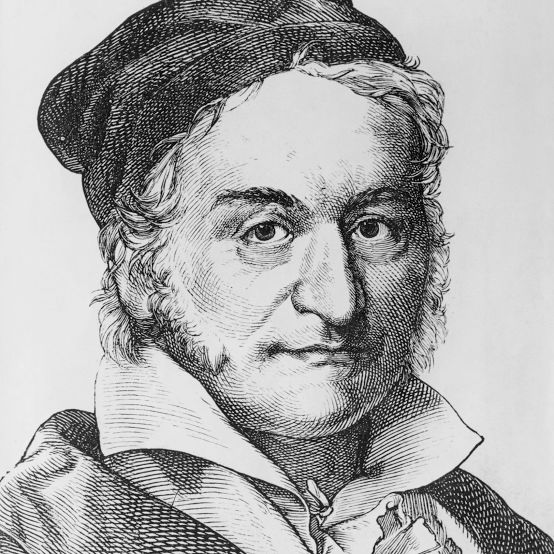
\includegraphics[width=1.0in]{images/gauss.jpeg}}
\caption*{\small ``The primes are the jewels in the crown.'' -- Carl Friedrich Gauss}
\end{figure}

\begin{figure}[ht]
\centerline{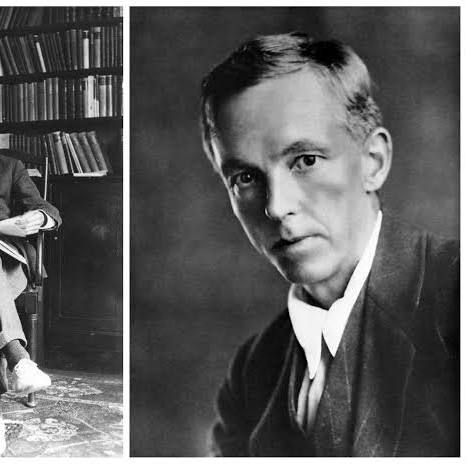
\includegraphics[width=1.0in]{images/Hardy.jpeg}}
\caption*{\small ``A mathematician, like a painter or a poet, is a maker of patterns. If his patterns are more permanent than theirs, it is because they are made with ideas. And the primes are the most eternal patterns of all.'' -- G. H. Hardy}
\end{figure}

\begin{figure}[ht]
\centerline{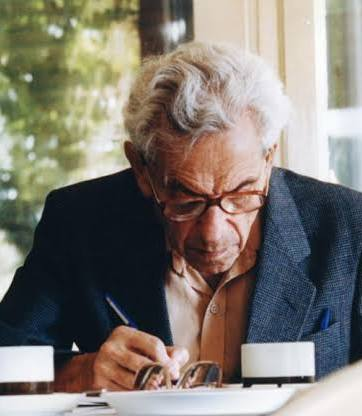
\includegraphics[width=1.0in]{images/Erdoss.jpeg}}
\caption*{\small ``God may not play dice with the universe, but something strange is going on with the prime numbers.'' --  Paul Erd\H{o}s}
\end{figure}

The theory of prime numbers and their properties forms the foundation of number theory.  At first sight, the study of primes may seem like a purely mathematical pursuit. 
Yet today prime numbers play a crucial role in modern life, because they underpin  cryptographic systems that secure communication over the internet. 

In this chapter we introduce the basic ideas of primes and factorisation, 
methods for computing greatest common divisors, some crucial algorithms and theorems about primes, 
and finally explain how these notions are used in public-key cryptography, especially the \href{https://en.wikipedia.org/wiki/RSA\_cryptosystem}{RSA cryptosystem}.

\section{Primes}

We have informally discussed primes several times in these notes. We give a formal definition here
\begin{definition}
A \emph{prime number} is an integer $p > 1$ whose only positive divisors are $1$ and $p$ itself.
\end{definition}

Numbers greater than 1 that are not prime are called \emph{composite}.  
$2,3,5,7,11$ are some examples of primes, while $12=3 \times 4$ is composite.  In what follows, we develop some properties of prime numbers.

\subsection{There are infinitely many primes}

In Theorem \ref{thm:infiniteprimes} we proved there are infinitely many primes. We repeat the theorem here for the sake of completeness.

\begin{theorem}[Euclid]
There are infinitely many prime numbers.
\end{theorem}
\begin{proof}
Suppose there are only finitely many: $p_1,\dots,p_k$. 
Consider $N=p_1\cdot p_2\cdots p_k+1$. 
No $p_i$ divides $N$, since each leaves remainder $1$. 
Thus $N$ is prime or divisible by a new prime, contradicting the assumption\footnote{Assume you have a finite list of primes. Multiply them together and add 1. Either that number is prime — or you just found a new factor. Either way, you’re wrong. Welcome to mathematics!}. 
\end{proof}
\vspace{2mm}

\subsection{Unique prime factorisation}

The  \emph{Unique Prime Factorisation theorem}  (Theorem \ref{thm:primefactor}) establishes that primes are the ``atoms'' of arithmetic: every integer factors into primes, and no further. We again repeat it here for completeness.
\begin{theorem}[Fundamental Theorem of Arithmetic]
Every integer $n>1$ can be written as a product of primes. 
This factorisation is unique up to the order of the factors.
\end{theorem}
\begin{proof}
\emph{Existence:} If $n$ is prime, we are done. Otherwise, assume that the claim is true for all $m$ such that $2 \leq m < n$. Let  $n=ab$ with $a,b<n$. By the induction hypothesis, each of $a$ and $b$ has a prime factorisation, hence so does $n$.

\emph{Uniqueness:} Suppose
\[
n = p_1p_2\cdots p_k = q_1q_2\cdots q_m
\]
with all $p_i, q_j$ prime. Then $p_1$ divides the right side, hence some $q_j$. But since $q_j$ is prime, $p_1=q_j$. Cancelling, we continue inductively to conclude that the multisets $\{p_i\}$ and $\{q_j\}$ are identical.
\end{proof}

\subsection{The Sieve of Eratosthenes}

One of the oldest known algorithms for finding prime numbers is due to 
\emph{Eratosthenes of Cyrene} (around 200 BCE). 
The method, called the \href{https://en.wikipedia.org/wiki/Sieve\_of\_Eratosthenes}{Sieve of Eratosthenes}, systematically eliminates 
composite numbers from a list, leaving only primes.

\begin{quote}
Sift the Two's and Sift the Three's: \\
The Sieve of Eratosthenes. \\
When the multiples sublime, \\
The numbers that remain are Prime. \\

\hspace{1.0in}	-- Anonymous
\end{quote}

\subsubsection*{The Algorithm}
To find all primes up to a given number $N$:

\begin{enumerate}
\item Write down the list of integers $2,3,4,\dots,N$.
\item Start with the first number $p=2$. It is prime.
\item Cross out all multiples of $p$ greater than $p$ itself in the list.
\item Find the next uncrossed number. This is the next prime. Set $p$ to this number and repeat Step 3.
\item Continue until $p^2 > N$. All remaining uncrossed numbers are prime.
\end{enumerate}

\begin{example}{Primes up to 30}

\begin{figure}[h]
\centering
\begin{tikzpicture}[>=stealth, x=1.1cm, y=1.1cm]
  % Style for number boxes
  \tikzstyle{num}=[draw, minimum width=7mm, minimum height=7mm, align=center]

  % Place numbers 2..30 in a 3x10 grid (10 per row)
  \foreach \n [count=\k from 1] in {2,...,30}{
    \pgfmathtruncatemacro{\col}{mod(\k-1,10)}
    \pgfmathtruncatemacro{\row}{floor((\k-1)/10)}
    \node[num] (N\n) at (\col,-\row) {\small \n};
  }

  % Cross out composites:
  % Multiples of 2 (>=4): red X
  \foreach \m in {4,6,8,10,12,14,16,18,20,22,24,26,28,30}{
    \draw[red, thick] (N\m.south west) -- (N\m.north east);
    \draw[red, thick] (N\m.south east) -- (N\m.north west);
  }

  % Multiples of 3 (>=6): blue diagonal (overlay)
  \foreach \m in {6,9,12,15,18,21,24,27,30}{
    \draw[blue, very thick] (N\m.south west) -- (N\m.north east);
  }

  % Multiples of 5 (>=10): green horizontal (overlay)
  \foreach \m in {10,15,20,25,30}{
    \draw[green!60!black, very thick] (N\m.west) -- (N\m.east);
  }

  % Legend
  \node[anchor=west] at (-0.2, -3.6) {\footnotesize \textbf{Legend:}};
  \draw[red, thick] (-0.2,-3.9) -- +(0.6,0);
  \node[anchor=west] at (0.5,-3.9) {\footnotesize multiples of 2};
  \draw[blue, very thick] (3.6,-3.9) -- +(0.6,0);
  \node[anchor=west] at (4.3,-3.9) {\footnotesize multiples of 3};
  \draw[green!60!black, very thick] (7.4,-3.9) -- +(0.6,0);
  \node[anchor=west] at (8.1,-3.9) {\footnotesize multiples of 5};
\end{tikzpicture}
\caption{Sieve of Eratosthenes up to 30. Uncrossed boxes are primes.}
\label{fig:sieve}
\end{figure}

Start with the numbers $2$ to $30$ (see Figure \ref{fig:sieve}).

\begin{itemize}
\item $2$ is prime. Cross out $4,6,8,\dots,30$.
\item Next uncrossed is $3$. Cross out $6,9,12,\dots,30$.
\item Next uncrossed is $5$. Cross out $10,15,20,25,30$.
\item Next uncrossed is $7$. Since $7^2=49>30$, we stop.
\end{itemize}

The remaining numbers are $2,3,5,7,11,13,17,19,23,29$, exactly the primes $\leq 30$.
\end{example}
\subsection*{Remarks}
\begin{itemize}
\item The sieve is simple and efficient for generating primes up to a moderately large bound.
\item It takes  $O(N \log \log N)$ steps for large $N$, making it far faster than testing each number individually for divisors.
\item This method, though ancient, is still used sometimes\footnote{Unfortunately, this algorithm is too inefficient in practice. The problem of primality testing -- how to test whether a given integer is a prime -- has been open  at least since the times of Euclid and Eratosthenes. The first ``efficient'' solution for the problem was the \href{https://en.wikipedia.org/wiki/AKS_primality_test}{AKS algorithm from IIT Kanpur} in 2002. In practice, an even faster \href{https://en.wikipedia.org/wiki/Miller–Rabin_primality_test}{Miller-Rabin test} is used, but it uses probabilistic coin tosses as a primitive, and can give a wrong answer with a very small probability. We will study some of these methods later in these otes}.
\end{itemize}

\begin{exercise}
Find all primes between 2 and 100 using the Sieve of Eratosthenes.
\end{exercise}

\subsection{The Prime Number Theorem}

The distribution of primes among the natural numbers is highly irregular: 
sometimes primes cluster close together, other times they are far apart. 
A natural question, posed already by \href{https://en.wikipedia.org/wiki/Carl\_Friedrich\_Gauss}{Gauss} and \href{https://en.wikipedia.org/wiki/Adrien-Marie\_Legendre}{Legendre} around the year 1800 when he was a teenager\footnote{Historians like to quip: ``Even at 15, Gauss preferred to keep his prime secrets private.''}, is:
\emph{How many primes are there up to a large number $n$?}

\begin{theorem}[\href{https://en.wikipedia.org/wiki/Prime\_number\_theorem}{Prime Number Theorem}]
\label{thm:primenumber}
Let $\pi(n)$ denote the number of primes $\leq n$. Then
\[
\pi(n) \sim \frac{n}{\ln n}, \quad \text{as } n \to \infty,
\]
meaning that
\[
\lim_{n\to\infty} \frac{\pi(n)}{n/\ln n} = 1.
\]
\end{theorem}

\begin{figure}[h]
\centering
\begin{tikzpicture}
\begin{semilogxaxis}[     % log scale on x-axis
    xlabel={$n$},
    ylabel={$\ln(n)$},
    width=12cm, height=7cm,
    log basis x=10,
    xtick={1,10,100,1000,10000,100000,1000000,10000000,100000000,1000000000,10000000000},
    xticklabels={$10^0$,$10^1$,$10^2$,$10^3$,$10^4$,$10^5$,$10^6$,$10^7$,$10^8$,$10^9$,$10^{10}$},
    ytick={0,5,10,15,20,25},
    grid=both
]
\addplot[domain=1:1e10, samples=500, thick, blue] {ln(x)};
\end{semilogxaxis}
\end{tikzpicture}
\caption{The natural logarithm $\ln(n)$ grows very slowly, even as $n$ reaches $10^{10}$.}
\label{fig:lnn}
\end{figure}


In words: the density of primes around $n$ is roughly $\tfrac{1}{\ln n}$.  The \href{https://en.wikipedia.org/wiki/Natural\_logarithm}{natural logarithm function} $\ln n$ is a rather slowly growing function. It can be intuitively understood as a way of answering the question: ``How much time does it take to grow from 1 to $n$, assuming continuous growth at a fixed rate?". See Figure \ref{fig:lnn} for a plot. We will revisit the natural logarithm function later in these notes. So, primes are not very sparse at all\footnote{Carl Friedrich Gauss (1792–93), as a teenager, investigated prime tables and conjectured the approximation $\pi(n) \approx \operatorname{Li}(n)$, where $\operatorname{Li}(n) = \int_2^n \tfrac{dt}{\ln t}$ is the logarithmic integral.  He recorded this insight in his diary, long before publishing it. Adrien-Marie Legendre independently proposed the formula $\pi(n)\approx \tfrac{n}{\ln n - 1.08366}$ in 1798. The theorem was finally proved independently in 1896 by \href{https://en.wikipedia.org/wiki/Jacques\_Hadamard}{Jacques Hadamard}  and \href{https://en.wikipedia.org/wiki/Charles\_Jean\_de\_la\_Vall\%C3\%A9e\_Poussin}{Charles Jean de la Vall\'ee Poussin}, using complex analysis and properties of the Riemann zeta function.   Their proof showed how deep connections between prime numbers and complex analysis truly are. Interested students will have to wait for a few later course in mathematics to study the proofs}.
For example, around $n=10^6$, about one in every $14$ numbers is prime.

The proof of the prime number theorem is unfortunately out of the scope of these notes. Interested readers will have to follow up QRMT with some courses on calculus, analysis and algebra for the proof to be accessible.

\begin{exercise}
Use a calculator to stimate the number of primes between $10^6$ and $10^7$ using the prime number theorem.
\end{exercise}


\subsection{Fermat’s Little Theorem}

Prime numbers have remarkable properties in modular arithmetic. 
One of the most beautiful and useful is a result discovered by \href{https://en.wikipedia.org/wiki/Pierre\_de\_Fermat}{Pierre de Fermat} in 1640, 
long before the modern development of number theory. 
It shows that when we raise a number to a large power, the remainder upon division by a prime 
behaves in a very simple way.

Fermat wrote that if $p$ is a prime and $a$ is not divisible by $p$, then
$a^{p-1} \equiv 1 \pmod p$. 
He gave no proof, and the first rigorous demonstrations came later from \href{https://en.wikipedia.org/wiki/Leonhard\_Euler}{Leonhard Euler} and others.

This theorem is central in number theory. 
It lies behind efficient algorithms for primality testing, 
and it forms one of the key mathematical tools used in public-key cryptography.
Before proving it, let us state it precisely.
\begin{theorem}[Fermat’s Little Theorem]
\label{thm:fermat}
If $p$ is prime and $p\nmid a$, then
\[
a^{p-1}\equiv 1 \pmod p.
\]
\end{theorem}
\begin{proof}
Multiplication by $a$ permutes the set $\{1,2,\dots,p-1\}$ modulo $p$ (why?)
Thus
\[
a\cdot 2a\cdots (p-1)a \equiv 1\cdot 2\cdot \cdots (p-1) \pmod p.
\]
This gives $a^{p-1}(p-1)!\equiv (p-1)! \pmod p$. Since $(p-1)!$ is not divisible by $p$, we may cancel to obtain $a^{p-1}\equiv 1 \pmod p$.
\end{proof}

\begin{exercise}
Argue that multiplication by $a$  permutes the set $\{1,2,\dots,p-1\}$ modulo $p$. That is, the operation is injective.
\end{exercise}


The Fermat's little theorem  can be used for primality testing as follows:

\subsubsection*{Fermat Primality Test Algorithm}

\begin{enumerate}
\item Given an integer \( n > 2 \), choose a random integer \( a \) where \( 1 < a < n-1 \) and \( \gcd(a, n) = 1 \).
\item Compute \( a^{n-1} \bmod n \).
\item If 
\[
a^{n-1} \not\equiv 1 \pmod{n},
\]
then \( n \) is definitely composite.
\item If 
\[
a^{n-1} \equiv 1 \pmod{n}
\]
holds for several randomly chosen values of \( a \), then \( n \) is probably prime.
\end{enumerate}

\subsubsection*{Limitations}
\begin{itemize}
\item The test is \emph{probabilistic}, not deterministic.
\item Certain composite numbers, known as \textit{Fermat pseudoprimes}, can satisfy the congruence for some bases \( a \), causing false positives.
\item To reduce error probability, test multiple values of \( a \) independently.
\end{itemize}

\begin{example}
For \( n = 11 \):
\[
2^{10} \equiv 1 \pmod{11}, \quad 3^{10} \equiv 1 \pmod{11},
\]
so 11 is probably prime.

For a composite number \( n = 15 \):
\[
2^{14} \not\equiv 1 \pmod{15},
\]
so 15 is composite.
\end{example}


\section{The Greatest Common Divisor}

\begin{figure}[ht]
\centerline{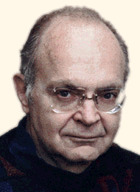
\includegraphics[width=1.0in]{images/don.jpg}}
\caption*{\small ``The Euclidean algorithm is one of the oldest nontrivial algorithms that has survived to the present day. It can be considered the first efficient algorithm ever devised.'' -- Donald Knuth}
\end{figure}

%\begin{figure}[ht]       
%\centerline{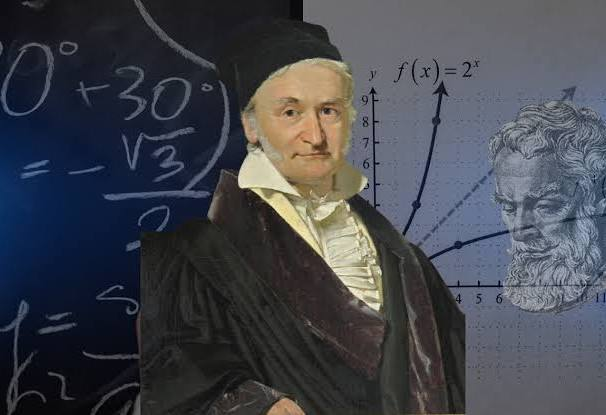
\includegraphics[width=1.0in]{images/gauss2.jpg}}
%\caption*{\small ``The algorithm of Euclid is the finest jewel in the crown of elementary number theory.'' -- Carl Friedrich Gauss}
%\end{figure}


When working with integers, one of the most natural questions is: given two numbers, 
what is the largest number that divides them both? For example, for $18$ and $24$ the answer is $6$, 
since $6$ is the largest integer that divides both without remainder. 
This simple idea is called the \emph{greatest common divisor}, or \emph{gcd} for short.

The gcd plays a central role in number theory. It captures the notion of 
the ``common part’’ of two numbers, and it is fundamental for simplifying fractions, 
solving equations in integers, and developing modular arithmetic. 
As we will see, the efficient algorithm to compute gcds, due to Euclid, 
is one of the oldest and most beautiful algorithms in all of mathematics.

\begin{definition}
The \emph{greatest common divisor} $\gcd(a,b)$ of two integers $a,b$ is the largest integer that divides both.
\end{definition}

\begin{example}
\[
\gcd(18,24)=6, \qquad \gcd(13,27)=1.
\]
\end{example}


\subsection{Euclid’s Algorithm}
Euclid, over 2000 years ago, discovered a remarkably efficient method, $Euclid\_gcd$, for computing $\gcd(a,b)$, $a > 0, b \geq 0$:
\begin{eqnarray*}
\begin{array}{ll}
Euclid\_gcd(a,b) = a & \mbox{if $b=0$} \\
Euclid\_gcd(a,b) = Euclid\_gcd(b,\, a \bmod b) & \mbox{otherwise}
\end{array}
\label{algo:Egcd}
\end{eqnarray*}
Repeating this step until the remainder is $0$ yields the gcd.

\begin{example}
To compute $\gcd(252,105)$:
\[
252=105\cdot2+42, \quad Euclid\_gcd(252,105)=Euclid\_gcd(105,42),
\]
\[
105=42\cdot2+21, \quad Euclid\_gcd(105,42)=Eucid\_gcd(42,21),
\]
\[
42=21\cdot2+0 \quad\Rightarrow\quad Euclid\_gcd(21,0) =21.
\]
\end{example}


\subsubsection{Correctness of Euclid's GCD algorithm}

To prove the correctness of Euclid's algorithm, we first require the following result which was
proved by Euclid. \newline
{\bf Claim:} If $a = qb + r$, $0 < r < b$, then $gcd(a,b) = gcd(b,r)$ \newline
\begin{proof}
If $d = gcd(a,b)$ then $d \mid a$ ($d$ divides $a$) and $d \mid b$ which, in turn, implies that
$d \mid (a - qb)$, or $d \mid r$. Thus $d$ is a common divisor of $b$ and $r$.
If $c$ is any common divisor of $b$ and $r$, then $c \mid (qb + r)$ which implies
that $c \mid a$. Thus $c$ is a common divisor of $a$ and $b$. Since $d$ is the largest
divisor of both $a$ and $b$, it follows that $c \leq d$.
It now follows from definition that $d = gcd(b,r)$.
\end{proof}

We can then prove the correctness of $Euclid\_gcd$ using the principle of mathematical induction.

\begin{theorem}
 For all $b \geq 0$, for all $a > 0$, $Euclid\_gcd(a,b)$ computes $\gcd(a,b)$, the largest common divisor of $a$ and $b$.
 \end{theorem}

\begin{proof}
\begin{description}
\item[Basis.] $b = 0$. If $b = 0$ then for all $a > 0$, 
      $Euclid\_gcd(a,b) = a = gcd(a,b)$.
\item[Induction hypothesis.] For all $b \leq k$ such that $0 \leq b$, for all $a > 0$,
         $Euclid\_gcd(a,b) = gcd(a,b)$.
\item[Induction step.] Consider $b = k+1$,  $a > 0$. 
         \[
         \begin{array}{llll}
         Euclid\_gcd(a,b) & = & Euclid\_gcd(b,a\;mod\;b) \\
                & = & gcd(b,a\;mod\;b) & \mbox{by the inductive hypothesis} \\
                & = & gcd(a,b) & \mbox{by the Claim above}
         \end{array}
         \]
\end{description}
\end{proof}


\begin{definition}
Two positive integers are  \emph{relatively prime} if their gcd is 1, i.e.,  they have no non-trivial factors in common.
\end{definition}

\subsection{The Extended Euclidean Algorithm}



Euclid’s algorithm is remarkable because it quickly computes the gcd of two numbers. 
But sometimes we need more than just the gcd: we want to write the gcd 
as a sum of multiples of the two numbers themselves\footnote{Euclid tells us what the gcd is; the extended Euclid tells us how to make it.}.

For example, for $a=30$ and $b=12$, not only is $\gcd(30,12)=6$, but also
\[
6 = 30 \times (-1) + 12 \times 3.
\]

In other words, the gcd can be expressed as a whole-number combination of $a$ and $b$.  This means we can “build” the gcd by taking suitable multiples of $30$ and $12$.
This fact is called \href{https://en.wikipedia.org/wiki/B\%C3\%A9zout\%27s_identity}{B\'ezout's identity}. 

The \emph{Extended Euclidean Algorithm} is just a way to find these multipliers
at the same time as we compute the gcd. 

\paragraph{How it works (idea).}
We start the same way as in Euclid’s algorithm:
\[
a = q_1 b + r_1, \quad b = q_2 r_1 + r_2, \quad \dots
\]
until we reach a remainder $0$.  
While we do this, we also keep track of how each remainder is made from $a$ and $b$.  
At the end, the last nonzero remainder is the gcd, and the numbers in front of $a$ and $b$ 
give us the multipliers we want.

\begin{figure}[ht]
\centerline{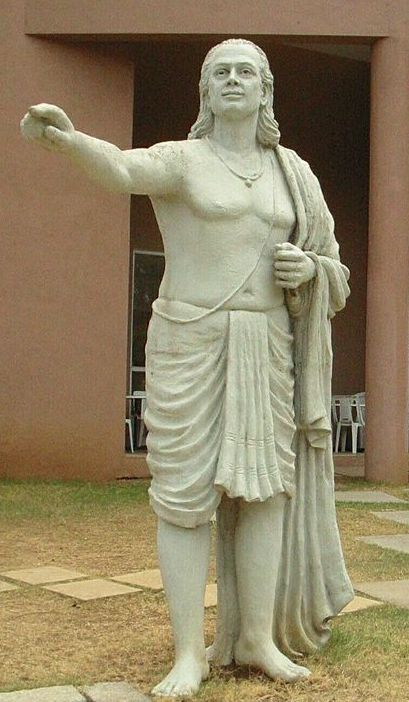
\includegraphics[width=1.0in]{images/Aryabhata_IUCAA.jpg}}
\caption*{\={A}ryabha\d{t}a's statue in the Inter-University Centre for Astronomy and Astrophysics (IUCAA) at Pune}
\end{figure}

\begin{example}
Let’s find the gcd of $26$ and $7$, and also write it as a combination of $26$ and $7$.

\[
26 = 3 \times 7 + 5, \quad
7 = 1 \times 5 + 2, \quad
5 = 2 \times 2 + 1, \quad
2 = 2 \times 1 + 0.
\]

So $\gcd(26,7)=1$.  

Now work backwards:
\[
1 = 5 - 2 \times 2,
\]
\[
1 = 5 - 2 \times (7 - 1 \times 5) = 3 \times 5 - 2 \times 7,
\]
\[
1 = 3 \times (26 - 3 \times 7) - 2 \times 7 = 3 \times 26 - 11 \times 7.
\]

So we have
\[
1 = 3 \times 26 + (-11) \times 7.
\]

This shows that $-11$ is a multiplier for $7$ that makes $7 \times (-11) \equiv 1 \pmod{26}$.  
In other words, $7$ has an inverse modulo $26$, and it is $15$ (since $-11 \equiv 15 \pmod{26}$) \footnote{We had discussed this earlier in Theorem \ref{thm:diaphontine}. The origins of this algorithm can be traced back to  \={A}ryabha\d{t}a ($5^{th}$ c), Jayadeva (c. $10^{th}$–$11^{th}$ c.) and later Bh\'{a}skara II ($12^{th}$ c.). Bh\'{a}skara in the L\={\i}l\={a}vat\={\i} and B\={\i}jaga\d{n}ita gives worked examples of solving linear Diophantine equations with what is recognizably the extended Euclid method.}.  
\end{example}

The steps of the general algorithm can then be given as:

\paragraph{General Algorithm (Extended Euclid).}

\label{algo:extended-Euclid}
Given two integers $a$ and $b$:

\begin{enumerate}
\item If $b=0$, then $\gcd(a,0)=a$ and we return $(x,y)=(1,0)$.
\item Otherwise, divide $a$ by $b$: 
\[
a = q b + r, \quad 0 \leq r < b.
\]
\item Inductively apply the algorithm to $(b,r)$ to get
\[
\gcd(b,r) = xb + yr.
\]
\item Substitute $r=a - qb$ to express the gcd in terms of $a$ and $b$:
\[
\gcd(a,b) = y a + (x - qy)b.
\]
\item Return $(x',y')=(y,\,x-qy)$.
\end{enumerate}

At the end, we obtain integers $x,y$ such that
\[
ax + by = \gcd(a,b).
\]

\begin{exercise}
(Bh\'{a}skara I, c. 600) ``Tell me at once, O mathematician, that number which leaves unity as remainder when divided by any of the numbers from 2 to 6 but is exactly divisible by 7." [Ans : 301]
\end{exercise}

\begin{exercise}
(Mah\={a}v\={\i}ra, c. 850) ``Five heaps of fruits added with two fruits were divided equally between nine travellers; six heaps added with four fruits were divided amongst eight; four heaps increased by one fruit were divided amongst seven. Tell the number of fruits in each heap.” [(Least) Ans : 194]
\end{exercise}

\paragraph{Why this matters.}
The extended Euclidean algorithm is very useful:
\begin{itemize}
\item It gives the gcd of two numbers.  
\item It shows how to write the gcd using those two numbers.  
\item If the gcd is $1$, it also finds a modular inverse, which is essential in cryptography.  
\end{itemize}

But how many steps does the Euclidean algorithm take? Is it slow or fast? Amazingly, the answer lies in the famous \href{https://en.wikipedia.org/wiki/Fibonacci_sequence}{Fibonacci sequence}\footnote{Though named after \href{https://en.wikipedia.org/wiki/Fibonacci}{Fibonacci}, also referred to as the {\em Leonardo of Pisa}, the sequence was known to ancient Indian mathematicians like \href{https://en.wikipedia.org/wiki/Pingala}{Pingala}, \href{https://en.wikipedia.org/wiki/Bharata\_(sage)}{Bharata muni}, \href{https://en.wikipedia.org/wiki/Virahanka}{Virahanka}, \href{https://en.wikipedia.org/wiki/Hemachandra}{Gopala and Hemachandra}.} defined as:
\[
\begin{array}{l}
F_0 = 0 \\
F_1 = 1 \\
F_k = F_{k-1} + F_{k-2}, \mbox{ for } i \geq 2
\end{array}
\]


The following theorem establishes the worst-case run rime of the Euclidean algorithm:

\begin{theorem}
If $a > b \geq 1$ and the invocation $Euclid\_gcd(a, b)$ performs $k \geq 1$ repeated calls, then $a \geq F_{k+2}$ and
$b \geq F_{k+1}$.
\end{theorem}

\begin{exercise}
Prove the above theorem using the principle of mathematical induction.
\end{exercise}

The following result immediately follows:
\begin{theorem}[Lam\'e's theorem]
For any integer $k \geq 1$, if $a > b \geq 1$ and $b < F_{k+1}$, then  $Euclid\_gcd(a, b)$ makes fewer than
$k$ repeated calls.
\end{theorem}

It is well known that $F_k \leq \phi^{k-1}$ for all $k > 0$, where $\phi = \frac{1+\sqrt{5}}{2}$ is the \href{https://en.wikipedia.org/wiki/Golden_ratio}{golden ratio}. 

\begin{exercise}
\begin{enumerate}
\item Prove that $F_k \leq \phi^{k-1}$ for all $k > 0$ using the principle of mathematical induction.
\item Argue that if  $b < F_{k+1} \leq \phi^k$, then the number of steps required will be approximately $\log{b}$, which is rather small. So, the algorithm is very efficient.
\end{enumerate}
\end{exercise}

\section{Chinese Remainder Theorem}


The Chinese Remainder Theorem (CRT) is one of the most beautiful and useful results in number theory. 
It says that if we know the remainder of a number when divided by several pairwise coprime moduli, 
then we can uniquely determine the number modulo the product of those moduli.

In other words, instead of working with a single large modulus, we can break a problem into 
several smaller ones, solve them separately, and then combine the answers back together. 
This is extremely powerful in computations, because working modulo small numbers is easier.

\medskip
\noindent
The theorem was discovered in ancient China, and first appeared in the work of 
Sun Tzu around the 3rd century AD, who posed problems like:
\emph{``Find a number which leaves remainder 2 when divided by 3, remainder 3 when divided by 5, and remainder 2 when divided by 7.''}  
The answer is unique modulo $3\cdot 5 \cdot 7 = 105$.

\medskip
\noindent
The CRT has many applications:
\begin{itemize}
\item Efficient computation in modular arithmetic (e.g. fast exponentiation).
\item Cryptography, especially RSA, where it is used to speed up decryption.
\item Error correction in coding theory.
\end{itemize}
Thus, the CRT is not only a striking piece of mathematics but also a practical tool.

\begin{example}{An example (\href{https://en.wikipedia.org/wiki/Sunzi_Suanjing}{Sun Tzu}, 3rd century AD).} \\

 ``There are certain things whose number is unknown. If we count them by threes, we have two left over; by fives, we have three left over; and by sevens, two are left over. How many things are there?” 


Suppose we want to find a number $N$ such that
\[
N \equiv 2 \pmod{3}, \quad 
N \equiv 3 \pmod{5}, \quad 
N \equiv 2 \pmod{7}.
\]

\noindent
Step 1. The moduli $3,5,7$ are pairwise coprime, so the CRT applies.  
The product is $M = 3 \cdot 5 \cdot 7 = 105$.

\smallskip
\noindent
Step 2. For each congruence, compute
\[
M_1 = \frac{M}{3} = 35, \quad 
M_2 = \frac{M}{5} = 21, \quad 
M_3 = \frac{M}{7} = 15.
\]

\smallskip
\noindent
Step 3. Find numbers $y_i$ such that
\[
M_1 y_1 \equiv 1 \pmod{3}, \quad 
M_2 y_2 \equiv 1 \pmod{5}, \quad 
M_3 y_3 \equiv 1 \pmod{7}.
\]

\begin{itemize}
\item $35 \equiv 2 \pmod{3}$, and $2\cdot 2 \equiv 1 \pmod{3} \implies y_1=2$.
\item $21 \equiv 1 \pmod{5}$, so $y_2=1$ works.
\item $15 \equiv 1 \pmod{7}$, so $y_3=1$ works.
\end{itemize}

\smallskip
\noindent
Step 4. Combine everything:
\[
N \equiv a_1 M_1 y_1 + a_2 M_2 y_2 + a_3 M_3 y_3 \pmod{M},
\]
where $(a_1,a_2,a_3)=(2,3,2)$.

\[
N \equiv 2 \cdot 35 \cdot 2 + 3 \cdot 21 \cdot 1 + 2 \cdot 15 \cdot 1 \pmod{105}.
\]

\[
N \equiv 140 + 63 + 30 = 233 \pmod{105}.
\]

\noindent
Step 5. Reduce: $233 \equiv 23 \pmod{105}$.

\medskip
\noindent
Therefore, the solution is 
\[
N \equiv 23 \pmod{105}.
\]

\smallskip
\noindent
Indeed, $23 \equiv 2 \pmod{3}$, $23 \equiv 3 \pmod{5}$, and $23 \equiv 2 \pmod{7}$.
\end{example}

\begin{theorem}[Chinese Remainder Theorem]
\label{thm:chinese}
Let $n_1,\dots,n_k$ be pairwise relatively prime  (i.e.\ $\gcd(n_i,n_j)=1$ for $i\neq j$), and $N=n_1\cdots n_k$. Then for any integers $a_1,\dots,a_k$ there is a unique solution $x \pmod N$ to
\[
x\equiv a_i \pmod{n_i}, \qquad i=1,\dots,k.
\]
\end{theorem}
\begin{proof}
Let $N_i=N/n_i$. Since $\gcd(N_i,n_i)=1$, there exists $y_i$ with $N_i y_i\equiv 1\pmod{n_i}$. 
Then $x=\sum a_i N_i y_i$ solves the congruences. Uniqueness follows: if $x$ and $x'$ are both solutions, then each $n_i$ divides $x-x'$, hence so does $N$.
\end{proof}

This also has an useful special form:

\begin{theorem}
Let $n_1,n_2,\dots,n_k$ be pairwise relatively prime, and let $N=n_1n_2\cdots n_k$. Then for all integers $x,a$,
\[
x \equiv a \pmod{n_i}\ \text{for each }i=1,2,\dots,k
\quad\Longleftrightarrow\quad
x \equiv a \pmod{N}.
\]
\end{theorem}

\begin{proof}
($\Rightarrow$) Assume $x \equiv a \pmod{n_i}$ for each $i$. Then $n_i \mid (x-a)$ for all $i$.
Since the $n_i$ are pairwise coprime, we claim that
\[
n_1n_2\cdots n_k \mid (x-a).
\]

Thus $x\equiv a\pmod{N}$.

\smallskip
($\Leftarrow$) Conversely, if $x\equiv a \pmod{N}$ then $n\mid(x-a)$. Since $n_i\mid N$, we have $n_i\mid(x-a)$ for each $i$, i.e.\ $x\equiv a\pmod{n_i}$ for all $i$.

\smallskip
This proves the equivalence.
\end{proof}

\begin{exercise}
(Yih-hiang, c. 700) ``Find the number of completed units of work, the same number of units to be performed by each of four sets of 2, 3, 6, 12 workmen, such that after certain whole days’ work, there remains 1, 2, 5, 5 units not completed by the respective sets.” [(Least) Ans : 17]
\end{exercise}

\section{Public-Key Cryptography}

From ancient times to the digital present, cryptography\footnote{See here for an \href{https://courses.cs.washington.edu/courses/cse490h1/19wi/exhibit/artifacts/crypto.pdf}{abridged history of cryptography.}} has carried with it an air of 
mystery and intrigue. In the past, emperors and generals relied on secret codes to 
protect messages from falling into enemy hands. The \href{https://en.wikipedia.org/wiki/Caesar\_cipher}{Caesar cipher}, for instance, shifted 
letters by a fixed number of places in the alphabet, and even such a simple trick was 
often enough to change the course of a battle, either way.

But as history has shown, secrecy is never easy to preserve. 
Every cipher invites the challenge of decryption: a contest between the code maker and 
the code breaker. This cat-and-mouse game gave rise to ingenious methods on both sides 
— from the \href{https://en.wikipedia.org/wiki/Bletchley\_Park}{codebreakers at Bletchley Park} during World War II, who cracked the \href{https://en.wikipedia.org/wiki/Enigma\_machine}{German 
Enigma machine}, to modern-day mathematicians working on factoring large numbers.

Public key cryptography is one of the most astonishing turns in this story. 
Until the 1970s, it was believed that secure communication required two parties to 
share a secret key in advance. The invention of public key cryptography overturned this 
assumption: it showed that two people could establish secure communication without ever 
having met before, using only openly published keys. 

This breakthrough was so surprising that it seemed almost paradoxical at first. 
How can one lock a message with a key that is public, and yet keep it safe from anyone 
but the intended recipient? The resolution lies in deep number theory, and in particular 
in the surprising difficulty of problems such as factoring large numbers. 
It is here that the elegance of mathematics meets the intrigue of secrecy.

In a public key cryptosystem, each participant has
\begin{itemize}
\item a \textbf{public key} (made widely known),
\item a \textbf{private key} (kept secret).
\end{itemize}
The public and the secret keys specify functions that can be
applied to any message $M$ which belongs to the set of permissible
messages ${\cal D}$.  The public and secret keys for a participant are a ``matched
pair'' in that they specify functions that are inverses of each other.
That is,
\[
\begin{array}{lll}
M & =  &S(P(M)), \\
M  &=  &P(S(M))
\end{array}
\]
for any $M \in {\cal D}$.
The challenge in designing a workable public-key cryptosystem is in figuring out how to create a system in which we can reveal a transformation $P()$, without thereby revealing how to compute the inverse transformation $S()$. Public-key cryptography solves this.

\subsection{How to encrypt?}

\begin{figure}[h]
\centering
\begin{tikzpicture}[
  node distance=4.5cm and 4.5cm,
  >=Stealth,
  every node/.style={font=\sffamily},
  box/.style={draw, rectangle, rounded corners, align=center, minimum width=3cm, minimum height=1cm}
]

% Nodes
\node[box] (bob) {Bob};
\node[box, right=of bob] (alice) {Alice};

\node[below=2cm of bob] (msg1) {Message $M$};
\node[below=2cm of alice] (msg2) {Decrypted $M = S_A(C)$};

% Encryption arrow
\draw[->, thick] (bob.east) -- node[above=0.3cm, align=center, text width=5cm]
{Encrypt $C = P_A(M)$ \\ using Alice's public key $P_A$} (alice.west);

% Decryption key note
\node[below right=0.6cm and -1.5cm of alice] (key) {Alice's secret key $S_A$};

% Dotted lines to show message association
\draw[dashed] (msg1.north) -- (bob.south);
\draw[dashed] (msg2.north) -- (alice.south);

\end{tikzpicture}
\caption{Encrypting a message with the receiver's public key.}
\end{figure}

Suppose Bob wishes to send a message $M$ to Alice, encrypted so that it will look like unintelligible gibberish to an eavesdropper. The procedure for doing so in a public-key cryptosystem is:

\begin{itemize}
\item Bob obtains Alice's key $P_A$, from a public directory, or directly from Alice.
\item Bob computes the \textit{ciphertext} $C = P_A(M)$, corresponding to the message $M$ and sends $C$ to Alice.
\item When Alice receives the ciphertext $C$, she applies her secret key $S_A$ to retrieve the original message: $M = S_A(C)$.
\end{itemize}

Since $S_A$ and $P_A$ are inverse functions, Alice can recover $M$ from $C$. Only Alice is able to compute $M$ from $C$, as only Alice knows $S_A$.

\subsection{Digital signature}

\begin{figure}[h]
\centering
\begin{tikzpicture}[
  node distance=4.5cm and 4.5cm,
  >=Stealth,
  every node/.style={font=\sffamily},
  box/.style={draw, rectangle, rounded corners, align=center, minimum width=3cm, minimum height=1cm}
]

% Nodes
\node[box] (alice) {Alice};
\node[box, right=of alice] (bob) {Bob};

\node[below=2cm of alice] (msg1) {Message $M'$};
\node[below=2cm of bob] (msg2) {Verification: $P_A(\sigma) \stackrel{?}{=} M'$};

% Signing arrow
\draw[->, thick] (alice.east) -- node[above=0.3cm, align=center, text width=5cm]
{Sign $\sigma = S_A(M')$ \\ using Alice's secret key $S_A$ \\ Send $(M',\sigma)$} (bob.west);

% Public key note
\node[below right=0.6cm and -1.5cm of bob] (key) {Alice's public key $P_A$};

% Dotted lines to show message association
\draw[dashed] (msg1.north) -- (alice.south);
\draw[dashed] (msg2.north) -- (bob.south);

\end{tikzpicture}
\caption{Digital signature: Alice signs the message $M'$ with her secret key to produce $\sigma=S_A(M')$. Bob verifies by checking $P_A(\sigma)=M'$ using the public key.}
\end{figure}

A signature is a device by which the receiver of the signed message can be assured of the identity of the sender and the integrity of the message. Digital signatures are fairly easy to implement in a public-key cryptosystem. Suppose Alice wishes to send Bob a digitally signed response $M'$. The procedure is as follows:

\begin{itemize}
\item Alice computes her \textit{digital signature} $\sigma$ for the message $M'$ using her secret key $S_A$ and the relation $\sigma = S_A(M')$.
\item Alice sends the message-signature pair $(M', \sigma)$ to Bob.
\item When Bob receives $(M', \sigma)$, he can verify that it came from Alice by using Alice's public key $P_A$ to verify the relation $M' = P_A(\sigma)$. (We presume that $M'$ contains Alice's name, so that Bob knows whose public key to use.) If the equation holds, then Bob concludes that Alice had sent it. If the equation does not hold, then he concludes that either $M'$ or $\sigma$ was corrupted by transmission errors, or $(M', \sigma)$ is an attempted forgery. Note that appending a digital signature necessarily increase the size of the total message.

\end{itemize}     

One can easily combine the two schemes to send signed and encrypted messages.

\begin{exercise}
Combine the two schemes above to derive a protocol for sending signed and encrypted messages.
\end{exercise}


\section{The RSA Cryptosystem}

\begin{figure}[h]
\begin{center}
\begin{tabular}{ccc}
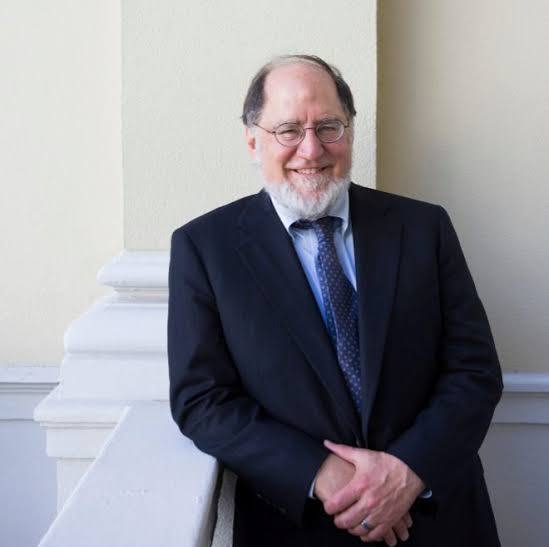
\includegraphics[width=1.0in]{images/rivest.jpeg} & 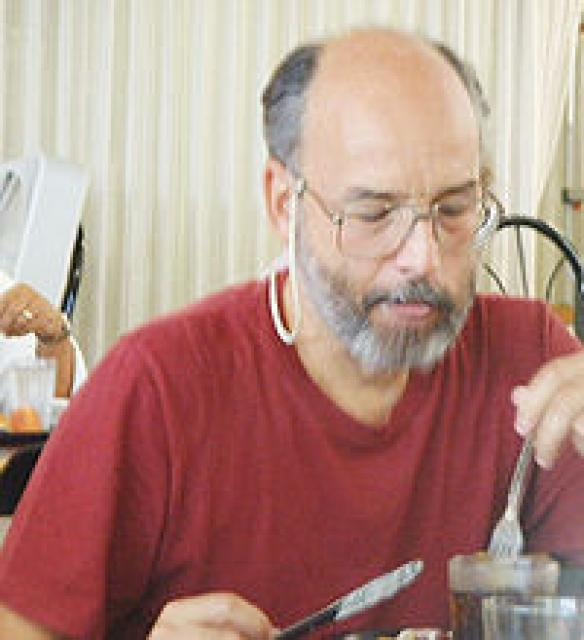
\includegraphics[width=0.9in]{images/adi-shamir-1.jpg} & 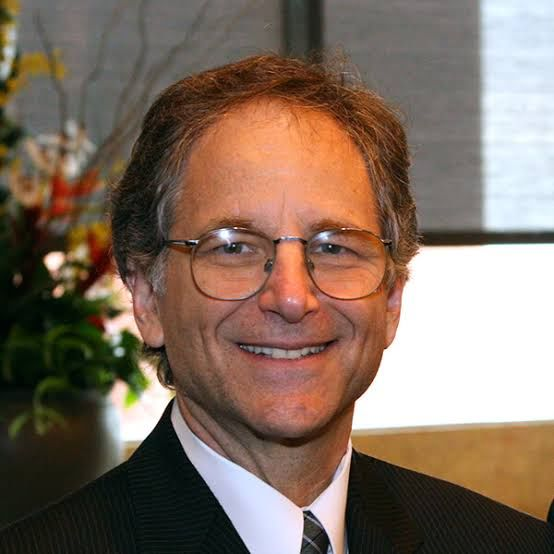
\includegraphics[width=1.0in]{images/adleman.jpeg} \\
Ronald Rivest & Adi Shamir & Leonard Adleman \\
\end{tabular}
\end{center}
\end{figure}
%\begin{figure}[ht]
%\centerline{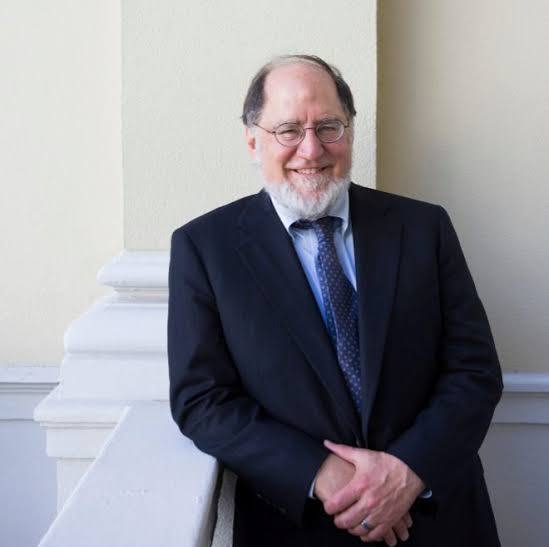
\includegraphics[width=1.0in]{images/rivest.jpeg}}
%\caption*{\small ``We stumbled on public-key cryptography almost by accident, but once we realized what we had, it was like discovering a new continent.'' -- Ron Rivest}
%\end{figure}
%
%\begin{figure}[ht]
%\centerline{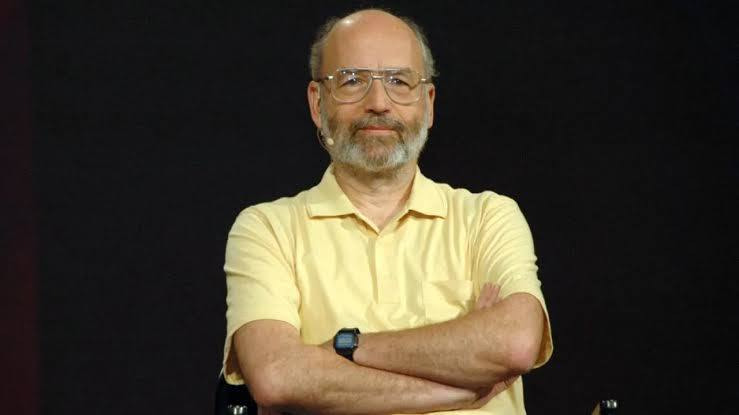
\includegraphics[width=1.0in]{images/shamir.jpeg}}
%\caption*{\small ``Cryptography is the only field where advances in pure mathematics can immediately create or destroy billions of dollars in value.'' -- Adi Shamir}
%\end{figure}
%
%\begin{figure}[ht]
%\centerline{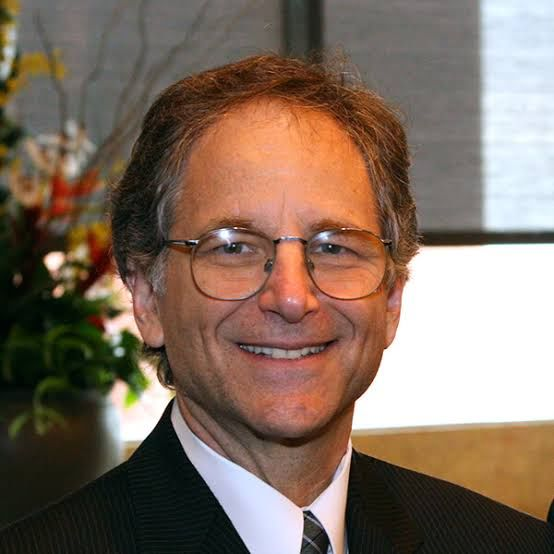
\includegraphics[width=1.0in]{images/adleman.jpeg}}
%\caption*{\small ``RSA worked because of a mathematical truth, not because anyone promised it would.'' -- Leonard Adleman}
%\end{figure}

The \href{https://en.wikipedia.org/wiki/RSA\_cryptosystem}{RSA cryptosystem} was proposed by \href{https://en.wikipedia.org/wiki/Ron\_Rivest}{Ronald Rivest}, \href{https://en.wikipedia.org/wiki/Adi\_Shamir}{Adi Shamir} and
\href{https://en.wikipedia.org/wiki/Leonard\_Adleman}{Leonard Adleman} in 1977. They got the \href{https://en.wikipedia.org/wiki/Turing\_Award}{Turing award} for their result in 2002.

\subsection{The RSA procedure}

To create his public and secret keys, a person uses the following procedure:

\begin{itemize}
\item Select two large prime numbers, $p$ and $q$, typically of 300 to 600 digits each. To select primes, choose random numbers of this size and test for primality using the Fermat's Little Theorem (Theorem \ref{thm:fermat}). By the Prime Number Theorem (Theorem \ref{thm:primenumber}) we are guaranteed to succeed in just a few trials.
\item Compute $n = pq$.
\item Select a small odd integer $e$ that is relatively prime to $m = (p-1)(q-1)$. Use Euclid's GCD to test whether a randomly chosen $e$ is relatively prime to $m$.
\item Compute $d$, the multiplicative inverse of $e$ modulo $m$.  Use the Extended Euclid Algorithm.
\item Publish the pair $P = (e,n)$ as his RSA public key.
\item Keep secret the pair $S = (d,n)$ as his RSA secret key.
\end{itemize}

For this scheme, the domain ${\cal D}$ is $\Z_n = \{0,1,\ldots,n-1\}$. That is,
the message $M$ must be such that $M \in  \Z_n$.The transformation of a message $M$ associated with a public key $P = (e,n)$ is \\
\[
P(M) = M^e \mod n
\]
The transformation of the ciphertext $C$ associated with a secret ket $S = (d,n)$ is \\
\[
S(C) = C^d \mod n
\]

These equations apply both to encryption and signatures.

\subsection{Why does it work?}
It is easy to see  that $P$ and $S$ are inverses:
\[
M^{ed} \equiv M \mod n
\]
\begin{proof}
Note that $m = (p-1)(q-1)$. Since $e$ and $d$ are multiplicative
inverses modulo $m$. We have that
\[
ed = 1 + km = 1 + k(p-1)(q-1)
\]
Thus if $M \not\equiv 0 \mod p$, we have that
\[
\begin{array}{lll}
M^{ed}  & \equiv & M(M^{p-1})^{k(q-1)} \mod p \\
        & \equiv & M(1)^{k(q-1)} \mod p  \\
        & \equiv & M \mod p 
\end{array}
\]
Note that $M^{p-1} \equiv 1 \mod p$ by Fermat's little theorem (Theorem \ref{thm:fermat}).

If $M \equiv 0 \mod p$, we anyway have that
\[
M^{ed} \equiv M \mod p
\]
Repeating the same argument as above, we have that
\[
M^{ed} \equiv M \mod q
\]
Hence, by the Chinese Remainder Theorem (Therem \ref{thm:chinese}) we have that
\[
M^{ed} \equiv M \mod pq \equiv M \mod n
\]
\end{proof}

\subsection{How secure is RSA?}

Multiplying two large primes to form $n$ is easy, but given only $n$ it is extremely difficult to recover $p$ and $q$ with current knowledge.  
RSA security relies on this asymmetry: the public modulus $n$ reveals nothing practical about the private key.  
At present, the only known way to obtain $d$ from $e$ and $n$ is to factor $n$ into its prime factors $p$ and $q$, then compute $m$ and proceed as
above. But no one knows how to factor large integers efficiently, despite several centuries of effort. Using known methods, factoring $n = pq$ where $p$
and q are 600-digit primes would require years on today's fastest supercomputers. Until someone comes up with an efficient way to factor, or discovers some
other way to compute $d$ from $e$ and $n$, the system is reasonably secure for all practical purposes.

RSA remains one of the most commonly use public-key encryption system in the digital world, including in banking, stock markets and other financial trasactions.


\section*{Summary}
\begin{itemize}
\item Primes are the building blocks of integers.
\item Euclid’s algorithm computes gcds efficiently.
\item There are infinitely many primes, and every integer has a unique prime factorisation.
\item Fermat’s little theorem and the CRT are central in modular arithmetic.
\item Public-key cryptography allows secure communication without prior key sharing.
\item RSA uses primes and modular arithmetic, with security based on the difficulty of factoring.
\end{itemize}

\section*{Problems}

\begin{enumerate}

\item \textbf{Prime numbers and factorisation}
  \begin{enumerate}
    \item Prove that there are infinitely many primes of the form $4k+3$.
    \item Factor $123456$ into primes using successive gcd computations.
    \item Use the sieve of Eratosthenes to list all primes up to $200$. 
          How efficient is this compared to trial division?
  \end{enumerate}

\item \textbf{Greatest common divisor}
  \begin{enumerate}
    \item Compute $\gcd(414,662)$ using Euclid’s algorithm. Show all intermediate steps.
    \item Use the extended Euclidean algorithm to find integers $x,y$ such that 
          $414x + 662y = \gcd(414,662)$.
  \end{enumerate}

\item \textbf{Fermat’s little theorem}
  \begin{enumerate}
    \item Verify Fermat’s little theorem for $a=7, p=13$.
    \item Show by counterexample that Fermat’s little theorem does not hold if $p$ is composite.
    \item Explain how Fermat’s little theorem can be used as a primality test. 
          What are its limitations?
  \end{enumerate}

\item \textbf{Chinese remainder theorem}
  \begin{enumerate}
    \item Solve the system of congruences:
      \[
        x \equiv 2 \pmod{3}, \quad 
        x \equiv 3 \pmod{5}, \quad 
        x \equiv 2 \pmod{7}.
      \]
      What is the smallest positive solution?
    \item A recent visitor to Ashoka University, Prof Amartya Kumar Dutta of ISI Kolkata gave the following problems:  
    \begin{enumerate}
    \item In a science camp of 210 students, creativity tests were planned in each of the subjects Mathematics, Physics and Chemistry. The students were to attempt the questions in groups of 5, 6 and 7 respectively. Unfortunately, a few students could not turn up due to unforeseen circumstances and it was found that dividing students into groups of 5, 6 and 7 would leave remainders 2, 1 and 5 respectively. Using ku\d{t}\d{t}aka, a professor of mathematics quickly realised how many students were present and suggested how the students could be grouped if uniformity in number was to be insisted. What was the total number of students present?
    \item (Hardy-Wright) From Monday, 1 January 2018, six professors begin two-year courses of lectures on Monday, Tuesday, Wednesday, Thursday, Friday, and Saturday. They announce their intention of lecturing at intervals of two, three, four, one, six, and five days respectively. However, no lecture is to take place on a Sunday and a professor would omit his lecture if it falls on a Sunday. For instance, the dates of the lectures of the first professor were January 1,3,5,9,11,13, … (omitting 7 January, a Sunday). What will be the date of the first Sunday on which all six professors find themselves compelled to omit a lecture?
    \end{enumerate}
    \item Explain why the Chinese Remainder Theorem is crucial for speeding up RSA decryption.
  \end{enumerate}

\item \textbf{Cryptography and RSA}
  \begin{enumerate}
    \item Work out a small RSA example: choose primes $p=17, q=23$, construct public/private keys, 
          and encrypt/decrypt the message $M=42$.
    \item Suppose Eve can factor the modulus $n$. Show why RSA becomes insecure.
    \item Consider the Caesar cipher. Implement it with shift $k=3$, encrypt the message ``HELLO'', 
          then decrypt it.
    \item Compare the Caesar cipher with RSA in terms of key space, security, and vulnerability to 
          brute-force attack.
  \end{enumerate}

\item \textbf{Reflection and open-ended problems}
  \begin{enumerate}
    \item Discuss why factoring large numbers is computationally difficult, and why this difficulty 
          underpins public-key cryptography.
    \item Research the Miller--Rabin primality test. How does it improve upon Fermat’s test?
    \item Find a real-world application where digital signatures are used. 
          Explain the role of public and private keys in that context.
  \end{enumerate}

\end{enumerate}

\chapter{Counting to Beat the Odds}

\begin{figure}[ht]       
\centerline{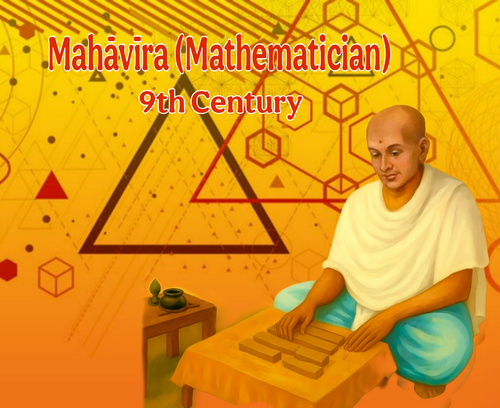
\includegraphics[width=1.0in]{images/mahavira.png}}
\caption*{\small ``There is no computation without the art of orderly enumeration.'' -- Paraphrased from Mah\={a}v\={\i}ra, \textit{Ga\d{n}itas\={a}rasa\d{n}graha} (9th century CE)}
\end{figure}

\begin{figure}[ht]       
\centerline{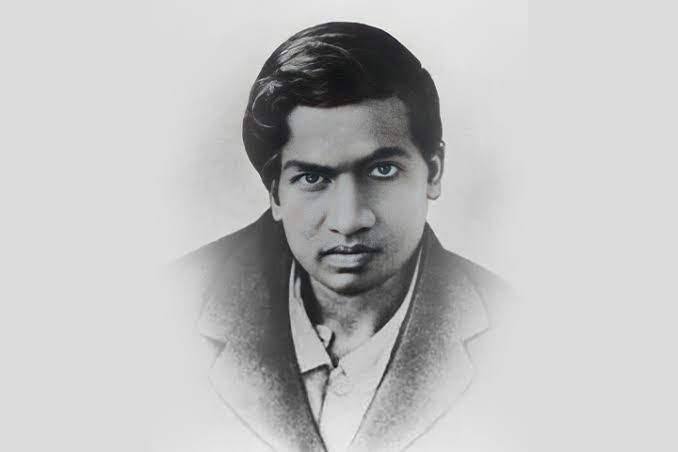
\includegraphics[width=1.0in]{images/ramanujan.jpeg}}
\caption*{\small ``There is no end to what can be counted; the more we count, the more we see patterns emerge.'' --  Paraphrased from the notebooks of Srinivasa Ramanujan}
\end{figure}


\section{Introduction}

Counting is one of the oldest and most universal human activities.
Long before the invention of symbols or written numbers, people used
stones, knots, or scratches on bones to keep track of livestock,
harvests, or trade. From these humble origins grew the entire
edifice of arithmetic, combinatorics, and probability theory.

In modern computer science and mathematics, counting is not merely an
act of enumeration but a way of understanding structure. How many
possible passwords of a given length can be formed? In how many distinct
ways can a set of vertices in a network be connected? In how many ways can certain objects be arranged? Each of these questions is,
at heart, a counting problem.

\medskip

The goal of this chapter is to develop systematic ways of counting the
number of possible outcomes in a finite discrete system, and then to
use these counts to reason about uncertainty and probability.

\begin{itemize}
  \item We first learn the \emph{basic counting principles}—the
  addition and multiplication rules—that form the backbone of all
  enumeration.
  \item We then study \emph{permutations} and \emph{combinations},
  which tell us how many ways elements can be arranged or selected.
%  \item The elegant yet deceptively powerful \emph{pigeonhole
%  principle} shows how counting can yield strong existence proofs.
\item We then study about the \emph{binomial theorem} and \emph{binomial coefficients}.
  \item Finally, we build upon these ideas to develop the foundations
  of \emph{discrete probability}—reasoning about likelihood when
  outcomes are finite and equally likely.
\end{itemize}

\section{The rules of sum and product}

\subsection{The rule of sum}
If a task can be done in $m$ ways, and another independent task can be
done in $n$ ways, and the two tasks cannot be done simultaneously,
then there are $m+n$ ways of choosing one of the two tasks.

\begin{example} 
\begin{enumerate}
\item Suppose you may take either a bus or a train to reach a city. If there
are 3 bus routes and 2 train routes, then there are $3+2=5$ ways to
travel.
\item Suppose the sections 1, 2 , and 3 of QRMT have 85, 90 and 88 students respectively. If we have to choose one class representative from the combined three sections, then there are $85 + 90 + 88 = 263$ ways
to choose the representative.
\end{enumerate}
\end{example}

\subsection{The rule of product}
If a task consists of two successive stages, the first of which can be
done in $m$ ways and the second in $n$ ways, then the entire task can
be done in $m \times n$ ways.

\begin{example}  
\begin{enumerate}
\item Suppose you must choose a shirt and a pair of trousers. If there are
4 shirts and 3 trousers, then there are $4 \times 3 = 12$ possible
outfits.
\item Suppose the sections 1, 2 , and 3 of QRMT have 85, 90 and 88 students respectively. If we have to choose one class representative from each of the three sections independently, then there are
$85 \times 90 \times 88 = 673200$ ways of choosing the three representatives.
\end{enumerate}
\end{example}

\section{Permutations}

\begin{definition}
A \emph{permutation} of a set of $n$ objects is an ordered arrangement
of all the objects. The number of permutations of $n$ objects is $n!$,
read as ``$n$ factorial'':
\[
n! = n \cdot (n-1) \cdot (n-2) \cdots 2 \cdot 1.
\]
\end{definition}

The first  can be chosen from $n$ objects, the second from the remaining $n-1$ objects, the third from the remaining $n-2$, and so on till 1.

\begin{example}
How many ways can 5 students line up for a photograph? \\
\emph{Solution:} There are $5! = 120$ possible line-ups.
\end{example}

Next, consider the number of ways of placing three balls coloured red, blue, and white in 10 boxes numbered $1,2,3,\ldots,10$, if each box can hold only one ball. The red ball can be placed in any of the 10 boxes, the blue ball can be place in any of the 9 remaining boxes, and the white ball can be placed in any of the remaining 8 boxes. Thus the total number of distinct ways to place these balls is $10 \times 9 \times 8 = 720$.

In general, if we have to place $r$ distinctly coloured balls in $n$ distinctly numbered boxes, then the number of distinct ways is
\[
n(n-1)(n-2) \cdots (n-r+1) =  \frac{n!}{(n-r)!}
\]

\begin{example}
\begin{enumerate}
\item In how many ways four examinations can be scheduled in a week so that no two examinations are scheduled on the same way? Considering the days as boxes and the examinations as distinct balls we obtain
the result as $7 \times 6 \times 5 \times 4 = 840$.
\item How many 3-digit numbers can be formed using the digits $\{1,2,3,4,5\}$ without repetition? Arguing similarly we arrive at  $5 \times 4 \times 3 = 60$.
\item How many four-digit decimal numbers can be formed without repeating the digits. This according to the above analysis is $10 \times 9 \times 8 \times 7 = 5040$. However, $9 \times 8 \times 7 = 504$ of them have 0 as the first digit. So, the number of distinct numbers that can be formed is $5040 - 504 = 4536$. We can also arrive at this result from the first principles by excluding 0 in the leading position. We then get the number of distinct numbers is $9 \times 9 \times 8 \times 7 = 4536$.
\end{enumerate}
\end{example}

An equivalent problem of placing distinct balls in boxes is that of arranging distinct objects. By permuting $r$ of $n$ distinct objects we mean to arrange $r$ of these $n$ objects in some order. For example, there are six ways to permute two out of three objects $a,b,c$. These are $ab,ba,ac,ca,bc,cb$. Arranging $r$ on $n$ objects amounts to filling $r$ positions with $r$ objects. We get the following definition:
\begin{definition}
\emph{Restricted permutations}: If only $r$ elements out of $n$ distinct elements are to be arranged, the number of permutations is
\[
P(n,r) = \frac{n!}{(n-r)!}.
\]
\end{definition}

\begin{example}
How many ways can 3 books be arranged on a shelf from a collection of 10?  
\[
P(10,3) = \frac{10!}{7!} = 720.
\]
\end{example}

\section{Counting functions and power sets}

Let us consider the problem of placing 3 distinctly coloured balls into 10 distinctly numbered boxes, but let a box hold as many balls as we wish. Since each of the red, blue, and the white ball can be placed in any of the 10 boxes the total number of ways is
\[
10 \times 10 \times 10 = 1000
\]
This is exactly the total number of functions that can be defined from the set of balls to the set of boxes.

In general, If there are $r$ distinct balls (the domain has $r$ elements) to be placed in $n$ distinct boxes (the co-domain has $n$ elements) and multiple balls can be mapped on to a box, then the total number of ways is $n^r$.

\begin{example}
Let us revisit the problem of scheduling four examinations in a week, but without any restrictions on number of examinations per day. This is exactly the problem of determining the number of functions that can be defined from the
courses to days of the week. The result is $7^4 = 2401$.
\end{example}

\begin{exercise}
Suppose that the popular tea company serve tea to their customers with 12 types of ingredients, each ingredient can be present or absent. How many different types of tea can they serve? 
\end{exercise}

\begin{exercise}
An $n$-bit binary number is defined as $b_0 + b_1 \times 2^1 + b_2 \times 2^2 + \ldots + b_{n-1} \times 2^{n-1}$, where each $b_i$ is 0 or 1. How many $n$-bit binary numbers are there? How many will have an even number of 1s?
\end{exercise}


\begin{exercise}
How many functions (truth tables) of $n$ boolean input and 1 boolean output can we define?
\end{exercise}

\subsection{Power set}
The Power set ${\cal P}(A)$ of a set $A$ is defined as the set of all subsets of $A$. For example, the set of all subsets of $A$ is ${\cal P}(A) = \left\{\phi, \left\{0\right\},  \left\{1\right\},  \left\{0,1\right\} \right\}$. Suppose the size of $A$ is
$r$. What is the size of ${\cal P}(A)$?

Consider the problem of placing each of the $r$ elements in two boxes -- inside the subset or outside. Since the $2^r$ ways of placing the $r$ elements, there are $2^r$ elements in ${\cal P}(A)$.


\section{Combinations} 

Consider now the problem of placing three balls, all red, in 10 boxes numbered $1,2,\ldots,10$. What are the total number of ways the balls can be placed if each box can hold at most one ball?

If the balls were of three shades of red, and hence distinguishable, then the answer would be $P(10,3)$. However, if  they are indistinguishable then $3!$ of the ways of their placement actually becomes one, and the number of ways reduces to $P(10,3)/3!$.

A problem equivalent to placing $r$ indistinguishable objects in $n$ numbered boxes is that of selection of $r$ objects from $n$ distinct objects. If we were to select $r$ objects from $n$, we can imagine the $n$ objects as boxes, and mark the selected ones. 

\begin{definition}
A \emph{combination} is a selection of objects without regard to order.
The number of combinations of $r$ objects chosen from $n$ is
\[
C(n,r) = \frac{n!}{r!(n-r)!}.
\]
\end{definition}
This is also sometimes denoted as $\binom{n}{r}$.

\begin{example}
\begin{enumerate}
\item Suppose Dining@Ashoka wants to schedule \emph{Tinda Kala Chana} at lunch three times a week. They can clearly do so in $\binom{7}{3} =  \frac{7!}{3!4!} = 35$ ways.
\item From 10 professors, in how many ways can a committee of 3 be chosen? The answer is $\binom{10}{3} = \frac{10!}{3! \, 7!} = 120$.
\end{enumerate}
\end{example}

\begin{exercise}
Clearly $\binom{n}{r} = \binom{n}{n-r}$. Give a combinatorial argument for the above.
 \end{exercise}
 \begin{example}
 \label{ex:rook}
Consider a $p \times q$ chess board. In how many ways a rook can move from the bottom-leftmost corner to the top-rightmost, moving only towards right and top? There are total  of $p-1$ right moves and $q-1$ top moves to be made. Think of them as red and blue balls respectively. Then, the problem is equivalent to the number of ways of choosing $p-1$ red balls from $p+q-2$ total balls, which is $\binom{p+q-2}{p-1}$. This is also exactly equal to $\binom{p+q-2}{q-1}$.
\end{example}


\begin{exercise}
Suppose we have to place $r$ balls in $n$ numbered boxes, where $q_1$ them are of one colour, $q_2$ of them are in second colour, $\ldots$, and $q_k$ of them are of the $k^{th}$ colour. Argue that the total number of ways to place the balls is
\[
\frac{P(n,r)}{q_1! q_2! \cdots q_k!}
\]
\end{exercise}

\begin{example}
\label{ex:rajan-suban}
Among 11 professors there are $C(11,5) = 462$ ways of selecting a committee of 5 members. Also, there are $C(10,4) = 210$ ways to select a committee of 5 members so that a particular professor, say professor Rajan, is always included, and there are $C(10,5) = 252$ ways of selecting a committee of 5 members so that professor Rajan is always excluded.  

We now ask in how many ways we can select a committee of 5 members so that at least one of prof Rajan and prof Suban will be included. The number of selections including both is $C(9,3) = 84$. The number of selections including Rajan but excluding Suban is $C(9,4) = 126$, as is the number of selections including Suban but excluding Rajan. Thus, the total number of ways is
\[
84+126+126 = 336
\]
Alternatively, since the total number of selections excluding both Rajan and Suban is $C(9,5)$, the total number of ways of selection is
\[
C(11,5) - C(9,5) = 462 - 126 = 336
\]
\end{example}

\subsection{Combination with repetitions}

Consider the problem of placing $r$ identical balls in $n$ numbered boxes, but allowing as many balls in a box as we wish. 

As an equivalent problem, consider the problem of arranging $n+1$ 1s and $r$ 0s with a 1 at the beginning and a 1 at the end of each arrangement. If we consider the 1s as inter-box partitions and 0s as balls, then every such arrangement is
a way of placing the $r$ balls in the $n$ boxes with possible repetitions. For example, let $ n= 5$, and $r = 4$. Then the sequence
\[
1011001101
\]
represents placing 1 ball in the first box, none in the second, 2 balls in the third box, none in the fourth, and 1 ball in the fifth box. The number of ways of arranging $r$ 0s and $n+1$ 1s with 1s at both ends is
\[
C(n+r-1,r) = \frac{(n+r-1)!}{r!(n-1)!}
\]

\begin{example}
\begin{enumerate}
\item The number of ways to select three days in a week with repetitions allowed is $C(9,3) = 84$.
\item The number of ways to select seven out of three days with repetitions allowed is $C(9,7) = 36$.
\item When three dices are rolled, the number of different outcomes is $C(8,3) = 56$.
\end{enumerate}
\end{example}
\section{The principle of Inclusion and Exclusion}

% ---------- Venn for two sets: inclusion–exclusion signs ----------
\begin{figure}[h]
\centering
\begin{tikzpicture}[scale=1.1, every node/.style={font=\small}]
  % Universe box
  \draw[rounded corners] (-3,-2) rectangle (3,2) node[anchor=south east] {$U$};

  % Circles A and B
  \def\r{1.5}
  \coordinate (cA) at (-0.9,0);
  \coordinate (cB) at ( 0.9,0);
  \draw[fill=black!8]  (cA) circle (\r);
  \draw[fill=black!8]  (cB) circle (\r);

  % Intersection hatch
  \begin{scope}
    \clip (cA) circle (\r);
    \fill[pattern=north east lines] (cB) circle (\r);
  \end{scope}

  % Set labels
  \node[anchor=south] at ($(cA)+(-0.2,\r)$) {$A$};
  \node[anchor=south] at ($(cB)+( 0.2,\r)$) {$B$};

  % PIE signs
  % Single-only regions (+)
  \node at ($ (cA)+(-0.65,0) $) {$+$};
  \node at ($ (cB)+( 0.65,0) $) {$+$};
  % Pairwise overlap (−)
  \node at ($ (cA)!0.5!(cB) $) {$-$};

  % Optional explanatory legend (comment out if not needed)
%  \node[align=left, anchor=north west] at (-2.8,-1.7) {%
%    \(\displaystyle |A\cup B|=|A|+|B|-|A\cap B|\)\\
%    \(\color{black}{+}\) singles,\ \(\color{black}{-}\) overlap
%  };
\end{tikzpicture}
\caption{The principle of inclusion and exclusion (2 sets).}
\label{fig:incl-excl-2}
\end{figure}
\begin{figure}[h]
\centering
\begin{tikzpicture}[scale=1.2, every node/.style={font=\footnotesize}]
  % Universe
  \draw[rounded corners] (-3.5,-3.0) rectangle (3.5,3.0);

  % Circle centers and radius
  \def\r{1.7}
  \coordinate (cA) at (-1,0.7);
  \coordinate (cB) at ( 1,0.7);
  \coordinate (cC) at ( 0,-1);

  % Fill each set lightly
  \draw[fill=black!10] (cA) circle (\r);
  \draw[fill=black!10] (cB) circle (\r);
  \draw[fill=black!10] (cC) circle (\r);

  % Pairwise overlaps (hatched)
  \begin{scope}
    \clip (cA) circle (\r);
    \fill[pattern=north east lines] (cB) circle (\r);
  \end{scope}
  \begin{scope}
    \clip (cA) circle (\r);
    \fill[pattern=north west lines] (cC) circle (\r);
  \end{scope}
  \begin{scope}
    \clip (cB) circle (\r);
    \fill[pattern=horizontal lines] (cC) circle (\r);
  \end{scope}

  % Triple overlap (darker)
  \begin{scope}
    \clip (cA) circle (\r);
    \clip (cB) circle (\r);
    \fill[black!30] (cC) circle (\r);
  \end{scope}

  % Set labels
  \node at ($(cA)+(0,\r+0.25)$) {$A$};
  \node at ($(cB)+(0,\r+0.25)$) {$B$};
  \node at ($(cC)+(0,-\r-0.20)$) {$C$};

  % Inclusion-Exclusion sign pattern
  \node at ($(cA)+(-0.9,0.1)$) {$+$};
  \node at ($(cB)+( 0.9,0.1)$) {$+$};
  \node at ($(cC)+( 0.0,-1.0)$) {$+$};

  \node at ($ (cA)!0.5!(cB) + (0,0.3) $) {$-$};
  \node at ($ (cA)!0.5!(cC) + (-0.3,-0.1) $) {$-$};
  \node at ($ (cB)!0.5!(cC) + (0.3,-0.1) $) {$-$};

  \node at ($(cA)!0.35!(cC)!0.5!(cB)$) {$+$};

  % Caption formula
%  \node[anchor=north west, align=left] at (-3.1,-2.3) {%
%    $|A\cup B\cup C| =$\\
%    $\quad |A|+|B|+|C|$\\
%    $\quad -(|A\cap B|+|A\cap C|+|B\cap C|)$\\
%    $\quad +|A\cap B\cap C|$};

\end{tikzpicture}
\caption{The principle of inclusion and exclusion (3 sets).}
\label{fig:incl-excl-3}
\end{figure}

The problem of Example \ref{ex:rajan-suban} can also be solved by the following method. Among the 462 ways of selecting the committee of 5, let $A_1$ and $A_2$ be the set of ways of selection that include Rajan and Suban respectively.  Now, since
\[
\begin{array}{l}
\mid A_1 \mid = C(10,4) = 210 \\
\mid A_2 \mid = C(10,4) = 210 \\
\mid A_1 \cap A_2 \mid = C(9,3) = 84 \\
\end{array}
\]
We. can estimate $\mid A_1 \cup A_2 \mid$, the number ways to include at least one of Rajan and Suban, as 
\[
\mid A_1 \cup A_2 \mid = \mid A_1 \mid + \mid A_2 \mid - \mid A_1 \cap A_2 \mid  = 210+210-84 = 336
\]
The last subtraction is necessary because the number of ways where both Rajan and Suban are included is double counted in $\mid A_1 \mid + \mid A_2 \mid$.  This method of counting is called the \emph{principle of inclusion and exclusion}.

For any two finite sets $A$ and $B$,
\[
|A \cup B| = |A| + |B| - |A \cap B|.
\]
The subtraction corrects for the double counting of elements common to both sets (See Figure \ref{fig:incl-excl-2}) .

\begin{example}
Let $A$ be the set of students taking Mathematics (40 students) and
$B$ be those taking Physics (30 students), with 10 students taking
both. Then, the size of the set taking at least one of Mathematics and Physics is
\[
|A \cup B| = 40 + 30 - 10 = 60.
\]
\end{example}


For three finite sets $A,B,C$,
\[
|A \cup B \cup C| =
|A| + |B| + |C|
- |A \cap B| - |A \cap C| - |B \cap C|
+ |A \cap B \cap C|.
\]

\begin{exercise}
Argue the correctness of the above formula (see Figure \ref{fig:incl-excl-3}).
\end{exercise}

We can generalize the above for $n$ sets $A_1, A_2, \ldots, A_n$ as,
\[
\left|\bigcup_{i=1}^{n} A_i\right|
= \sum_{i} |A_i|
- \sum_{i<j} |A_i \cap A_j|
+ \sum_{i<j<k} |A_i \cap A_j \cap A_k|
- \cdots + (-1)^{n+1} |A_1 \cap A_2 \cap \cdots \cap A_n|.
\]

\begin{example}[Derangements]
How many permutations of $\{1,2,3\}$ have no fixed point (i.e., no
element appears in its original position)?  
Let $A_i$ denote the set of permutations that fix $i$.  
\[
|A_1|=|A_2|=|A_3|=2,\quad
|A_i \cap A_j|=1,\quad
|A_1 \cap A_2 \cap A_3|=1.
\]
Thus,
\[
|\overline{A_1 \cup A_2 \cup A_3}| =
3! - (3\times2) + (3\times1) - 1 = 6 - 6 + 3 - 1 = 2.
\]
Hence, there are 2 derangements.
\end{example}

\begin{example}
Suppose an Ashoka student wants to make up a schedule for a seven-day period during which she will study only one subject each day. She is taking four subjects - Environmental Studies (EVS), Great Books (GB), Economic Politics and Society (EPS) and Quantitative Reasoning and Mathematical Thinking (QRMT). Clearly, there are $4^7$ different schedules. We want to know the number of schedules that devote at least one day to each subject?

Let $A_1$ denote the set of schedules in which EVS is never studied; likewise $A_2$, $A_3$, $A_4$ for GB, EPS, and QRMT respectively. Then,
\[
A_1 \cup A_2  \cup A_3  \cup A_4
\]
is the set of schedules in one or more of the subjects is not included.
Since
\[
\begin{array}{l}
\mid A_1 \mid = \mid A_2  \mid = \mid A_3  \mid =  \mid A_4 \mid = 3^7 \\
\mid A_1 \cap A_2 \mid = \mid A_1 \cap A_3 \mid = \mid A_1 \cap A_4 \mid = \mid A_2 \cap A_3 \mid =  \mid A_2 \cap A_4 \mid = \mid A_3 \cap A_4 \mid = 2^7 \\
\mid A_1 \cap A_2 \cap A_3 \mid = \mid A_1 \cap A_2 \cap A_4 \mid =  \mid A_1 \cap A_3 \cap A_4 \mid = \mid A_3 \cap A_3 \cap A_4 \mid = 1^7 \\
\mid A_1 \cap A_2 \cap A_3 \cap A_4 \mid = 0 \\
\end{array}
\]
We obtain
\[
\mid A_1 \cup A_2  \cup A_3  \cup A_4 \mid = 4(3^7) - 6(2^7) + 4
\]
\end{example}
Consequently, the number of schedules in which all subjects will be included is
\[
4^7 - (4(3^7) - 6(2^7) + 4)
\]
\begin{exercise}
Convince yourself $P(7,4)*4^3$ -- there are $P(7,4)$ ways to schedule 4 subjects for 4 of the 7 days, and $4^3$ ways to schedule three subjects for the remaining three days -- is not the correct answer.
\end{exercise}

\section{Recurrences: Counting by Relations}

Consider the following algorithms for sorting a list of integers in ascending order. Suppose we start with a sequence in random order such as
\[
\mid 8 \;3\;5\;9\;7
\] 
The symbol $\mid$ denotes that the elements to the right are unsorted. At the first step we can search through the list for the minimum element, and swap it with the element in the first position. We obtain a sorted part and an unsorted part
\[
3\mid8\;5\;9\;7
\]
Then, keeping the sorted part fixed, we can search through the rest of the list for the minimum element and swap it with the first element in the unsorted part to obtain
\[
3\;5\mid8\;9\;7
\]
Repeating the process we obtain in a sequence
\[
3\;5\;7\mid 9\;8
\]
and
\[
\begin{array}{l}
3\;5\;7\;8\mid 9 \\
3\;5\;7\;8\; 9 \mid
\end{array}
\]
Our problem is to count the number of comparisons required to sort a random sequence of $n$ elements.  

We can do this using the principle of mathematical induction. Let $T(n)$ be the number of comparisons required to solve a sorting problem of size $n$. If $n = 1$ then the sequence is sorted by default. Otherwise, we need to search
through $n$ elements to find the minimum which requires $n - 1$ comparisons, and are left with an identical subproblem of size $n-1$ which forms the induction hypothesis $T(n-1)$. Hence,
\[
T(n) = \left\{ 
            \begin{array}{ll}
            0 & \mbox{if $n = 1$} \\
            T(n-1) + (n-1) & \mbox{if $n > 1$}
            \end{array}
           \right.
\]
The above is called a \emph{recurrence relation}. We can solve this by telescoping
\[
\begin{array}{lll}
T(n) & = & T(n-1) + (n-1) \\
        & = & T(n-2) + (n-2) + (n-1) \\
        & \vdots & \vdots \\
         & = & T(1) + 1 + 2 + \ldots + (n-1) \\
         & = &  1 + 2 + \ldots + (n-1) = n(n-1)/2
\end{array}
\]
Thus we require $n(n-1)/2$ comparisons.


A \emph{recurrence relation} defines a sequence by relating each term to earlier ones.
Recurrences arise naturally in counting when a choice splits a problem into
smaller subproblems.  In fact, all counting problems can be expressed through recurrences. Consider the following examples.

\begin{example}
Consider the counting problem of number of distinct ways of arranging $n$ objects. There is only one way to arrange an empty set of objects, which forms the base case $P(0) = 1$. Suppose $P(n-1)$ is the number of ways
of arranging $n-1$ objects for $n > 0$ (the induction hypothesis). Then, the $n^{th}$ object can be inserted in each of the $P(n-1)$ arrangements in $n$ ways. Thus we have
\[
P(n) = \left\{ 
            \begin{array}{ll}
            1 & \mbox{if $n = 0$} \\
            n * P(n-1)  & \mbox{if $n > 0$}
            \end{array}
           \right.
\]

which evaluates to $P(n) = n!$
\end{example}
\begin{example}
Consider the rook problem of Example \ref{ex:rook}. In how many ways a rook can move from the bottom-leftmost corner to the top-rightmost in a $p \times q$ chessboard, moving only towards right and top? If $p = 1$ or $q = 1$ (a 1-dimensional chessboard), then there clearly is only one way giving us our base case. Otherwise, by the rule of sum, it is the sum of the total number of ways by taking the first step towards the right and the total number of ways by taking the first step towards the top. We obtain
\[
Rook(p,q) = \left\{ 
            \begin{array}{ll}
            1 & \mbox{if $p = 1$ or $q = 1$} \\
             Rook(p-1,q) + Rook(p,q-1) & \mbox{otherwise}
            \end{array}
           \right.
\]
Note that $Rook(p-1,q)$ and $Rook(p,q-1)$ are identical subproblems of smaller sizes, and hence are valid induction hypotheses. We saw earlier that this must be equal to $\binom{p+q-2}{p-1} = \binom{p+q-2}{q-1}$.
\end{example}

\subsection{\href{https://mathworld.wolfram.com/PascalsTriangle.html}{Pascal's triangle}}
The fact that the above recurrence evaluates to a combination suggests that  combination may itself be expressed as a recurrence. Consider the problem of selecting $r$ identical balls from $n$ boxes without repetition. Clearly,
if $r=0$ or $r=n$ we have exactly one way, giving our bases cases as $C(n,0) = C(n,n) = 1$. Now, by the rule of sum, the total number of ways of selecting is equal to the sum of the total number of ways of selecting by picking one from the $n^{th}$ box and the total number of ways by not picking at all from the $n^{th}$ box. This gives us
\[
C(n,r) = \left\{ 
            \begin{array}{ll}
            1 & \mbox{if $r = 0$ or $r = n$} \\
             C(n-1,r-1) + C(n-1,r) & \mbox{otherwise}
            \end{array}
           \right.
\]

The above recurrence leads us to the famous triangle of numbers called the \href{https://mathworld.wolfram.com/PascalsTriangle.html}{Pascal's triangle}\footnote{The triangular arrangement of binomial coefficients is commonly associated
with Blaise Pascal, whose posthumous work (1665) presented it systematically.
However, the structure was known much earlier. The Italian algebraist 
Niccol\`o Tartaglia published its first six rows in 1556. Even earlier, it
appeared in the writings of the Chinese mathematician Y\`ang Hu\`i and in the
work of the Persian scholar Omar Khayy\=am. Consequently, the triangle is known
by different names in different traditions:  Y\`ang Hu\`i triangle in China,
Khayy\=am's triangle in Persia, and Tartaglia's triangle in Italy.}.

Starting with $n=0$ the triangle is
\[
\begin{array}{lllllll}
1 \\
1 & 1 \\
1 & 2 & 1 \\
1 & 3 & 3  & 1 \\
1 & 4 & 6  & 4  & 1 \\
1 & 5 & 10 & 10 & 5 & 1 \\
1 & 6 & 15  & 20  & 15 &  6 &  1 
\end{array}
\]
Note that each number $\binom{n}{r}$ can be obtained by adding the two to the top and left in the previous row. Instead of computing $n!$ and $r!$ which are rather inefficient, the triangle gives faster method of computing $\binom{n}{r}$.

\begin{exercise}
A curious fact about the Pascal's triangle is that is we start from each of the 1s in the first column and add up the numbers along the anti-diagonals (in the direction $\nearrow$), then we obtain the Fibonacci numbers.  For example
\[
\begin{array}{l}
1 \\
1 \\
1 + 1 = 2\\
1 + 2 = 3 \\
1 + 3 + 1 = 5 \\
1 + 4 + 3 = 8 \\
1 + 5 + 6 + 1 = 13 \\
1 + 6 + 10 + 4 = 21 \\
\vdots
\end{array}
\]

Can you figure out why?
\end{exercise}

\begin{example}
 A shop keeper in the Asawarpur village adjoining Ashoka university thought of the following problem: 
      how many ways can one make a change of \rupee 1, given coins of 
      denomination 50p, 25p, 10p, 5p and 1p? More generally, can one write a 
      function to compute the number of ways to change any given amount of 
      money?  After giving some thought to the problem she noted that the 
      total number of ways to make change for some amount is equal to the 
      number of ways to make change for the amount without using any of the 
      first kind of coin, plus the number of ways to make change assuming we 
      do use a coin of the first kind. But the latter number is equal to the 
      number of ways to make change for the amount that remains after using 
      one coin of the first kind.  With this solution in mind she approached 
      the students of QRMT  for a recurrence for the problem. 
      Assume that there is a 
      function $d: \N \rightarrow \N$ that given you the denomination
      of the $n^{th}$ type of coin (for example, $d(1) = 1$, $d(2)=25$, $d(3) = 10$, $d(4)=5$ and
      $d(5) = 50$)\footnote{This is a special case of a general class of problems called the \href{https://en.wikipedia.org/wiki/Integer_partition}{partition problem}}.
\end{example}
\begin{exercise}
Suppose the amount for which change has to be generate is $a$. Argue that a solution to the counting problem is given by the following recurrence.
\[
Coin(a,n) = \left\{ 
            \begin{array}{ll}
            0 & \mbox{if $a < 0$ or $n = 0$} \\
             Coin(a,n-1) + Coin(a-d(n),n) & \mbox{otherwise}
            \end{array}
           \right.
\]

\end{exercise}


\section{The Binomial Theorem}\label{sec:binomial-theorem}

When we expand an expression of the form $(x+y)^n$ for a positive integer $n$,
we obtain a sum of products involving powers of $x$ and $y$. For small $n$, we
can compute these expansions by hand:
\[
(x+y)^2 = x^2 + 2xy + y^2, \qquad
(x+y)^3 = x^3 + 3x^2y + 3xy^2 + y^3.
\]
A clear pattern emerges: each term consists of a power of $x$ multiplied by a
power of $y$, and the coefficients follow the rows of Pascal's triangle. The
binomial theorem makes this pattern precise, expressing $(x+y)^n$ as a sum in
which the coefficients are exactly the binomial numbers $\binom{n}{k}$.

\begin{theorem}[Binomial Theorem]
For any integer $n \ge 0$ and for all commuting symbols or numbers $x,y$,
\[
(x+y)^n = \sum_{k=0}^{n} \binom{n}{k}\, x^{\,n-k} y^{\,k}.
\]
\end{theorem}

\begin{proof} ({\bf A combinatorial proof})
Expand $(x+y)^n$ as a product of $n$ identical factors:
\[
(x+y)^n = (x+y)(x+y)\cdots(x+y).
\]
A term $x^{\,n-k}y^{\,k}$ is formed by choosing $y$ from exactly $k$ of the $n$
factors and choosing $x$ from the remaining $n-k$ factors. The number of ways to
choose which $k$ factors contribute the $y$ is $\binom{n}{k}$. Thus,
\[
(x+y)^n = \sum_{k=0}^{n} \binom{n}{k}\, x^{\,n-k} y^{\,k}.
\]
\end{proof}

\begin{proof} ({\bf An inductive proof})
We prove the identity by induction on $n$.

\emph{Base case:} $n=0$. $(x+y)^0 = 1$ agrees with the right-hand side.

\emph{Inductive step:} 
Assume that for some $n \ge 0$,
\[
(x+y)^n = \sum_{k=0}^{n} \binom{n}{k} x^{\,n-k} y^{\,k}. \tag{$\ast$}
\]
We prove the identity for $n+1$.

\[
(x+y)^{n+1}
= (x+y)(x+y)^n
= (x+y)\sum_{k=0}^{n} \binom{n}{k} x^{\,n-k} y^{\,k}.
\]

Distribute:
\[
(x+y)^{n+1}
= \sum_{k=0}^{n} \binom{n}{k} x^{\,n+1-k} y^{\,k}
  + \sum_{k=0}^{n} \binom{n}{k} x^{\,n-k} y^{\,k+1}. \tag{1}
\]

We now \emph{reindex} the second sum. Let $j = k+1$. Then when $k=0$, $j=1$,
and when $k=n$, $j=n+1$. Also $k = j-1$. Therefore:
\[
\sum_{k=0}^{n} \binom{n}{k} x^{\,n-k} y^{\,k+1}
= \sum_{j=1}^{n+1} \binom{n}{\,j-1\,} x^{\,n-(j-1)} y^{\,j}
= \sum_{j=1}^{n+1} \binom{n}{\,j-1\,} x^{\,n+1-j} y^{\,j}. \tag{2}
\]

Now substitute $(2)$ into $(1)$ and combine the sums by matching powers:
\[
(x+y)^{n+1}
= \binom{n}{0} x^{\,n+1}
  + \sum_{j=1}^{n} \left(\binom{n}{j} + \binom{n}{j-1}\right) x^{\,n+1-j} y^{\,j}
  + \binom{n}{n} y^{\,n+1}. \tag{3}
\]

\medskip
Finally, we apply \textbf{Pascal's identity}:
\[
\binom{n}{j} + \binom{n}{j-1} = \binom{n+1}{j}.
\]

Substituting this into $(3)$ gives:
\[
(x+y)^{n+1}
= \sum_{j=0}^{n+1} \binom{n+1}{j} x^{\,n+1-j} y^{\,j}.
\]

This is exactly the binomial expansion for $(x+y)^{n+1}$, completing the induction.
\[
\boxed{(x+y)^n = \sum_{k=0}^{n} \binom{n}{k} x^{\,n-k} y^{\,k} \text{ for all } n \ge 0.}
\]
\end{proof}

\subsection*{Corollaries}
\begin{enumerate}
  \item $(1+1)^n = \sum_{k=0}^{n}\binom{n}{k} = 2^{n}$. (Give a purely combinatorial argument for this identity.)
  \item $(1-1)^n = \sum_{k=0}^{n}(-1)^k\binom{n}{k} = 0$ for $n \ge 1$.
  \item The coefficient of $x^{\,n-k}y^{\,k}$ in $(x+y)^n$ is $\binom{n}{k}$.
\end{enumerate}

\begin{example}
Using the binomial theorem,
\[
(2x - 3)^4
= \sum_{k=0}^{4} \binom{4}{k} (2x)^{4-k} (-3)^k
= 16x^4 - 96x^3 + 216x^2 - 216x + 81.
\]
\end{example}

\section{Discrete Probability}

Probability provides a mathematical language for reasoning about uncertainty.
Everyday situations such as tossing a coin, rolling a die, shuffling cards,
choosing passwords, or hashing data involve outcomes that cannot be predicted
with certainty in advance. Yet, they are not completely unpredictable: the set
of all possible outcomes is known, and many useful questions concern the
\emph{likelihood} of particular events. In this section we develop a framework
for thinking systematically about such situations.

We begin by describing random experiments and their sample spaces, and how
events are formed from outcomes. We then introduce probability measures and the
basic axioms that govern them. Next, we discuss random variables, which allow
us to assign numerical values to outcomes and reason about distributions,
independence, and conditional probabilities. Bayes' theorem provides a powerful
tool for updating beliefs in the light of new information. Finally, we conclude
with the concepts of information and entropy, which quantify uncertainty and
play a central role in modern data science, coding theory, and learning systems.

\subsection{Experiments, Sample Spaces, and Events}

A \emph{random experiment} is a process whose outcome cannot be predicted with
certainty in advance, even though all possible outcomes are known.
The set of all possible outcomes is called the \emph{sample space}, denoted $S$.
An \emph{event} is a subset $E \subseteq S$.

\begin{example}
\begin{enumerate}
  \item Tossing a fair coin: $S = \{\text{H}, \text{T}\}$.
  \item Rolling a fair die: $S = \{1,2,3,4,5,6\}$.
  \item Drawing a card from a standard deck of 52 cards.
\end{enumerate}
\end{example}

Two events $A$ and $B$ are \emph{mutually exclusive} if $A \cap B=\varnothing$.
A collection of events $A_1, \dots, A_k$ is \emph{exhaustive} if
$A_1 \cup A_2 \cup \cdots \cup A_k = S$.

\subsection{Probability Measure and Axioms}

A \emph{probability measure} assigns to each event $E\subseteq S$ a number
$P(E)$ satisfying:
\[
P(E)\ge 0,\qquad P(S)=1,\qquad.
\]

When $S$ is finite and all outcomes are equally likely,
\[
P(E)=\frac{|E|}{|S|}.
\]

\begin{example}
\begin{enumerate}
  \item $P(\text{even number when rolling a die}) = \frac{3}{6} = \frac{1}{2}$.
  \item $P(\text{ace from a deck}) = \frac{4}{52} = \frac{1}{13}$.
  \item Consider the problem of dealing a poker hand out of a deck of cards. The sample space consists of $C(52,5)$ different hands that can be dealt. We assume that all of these are equally probable. What is the
          probability of getting four aces? We note that 48 possible outcomes from the sample space contain 4 aces (1 way to choose 4 aces and 48 ways to choose the remaining card). So, the probability is
          $48/C(52,5) = 0.0000185$.
  \item What is the probability that in the QRMT class of 88 students, no two have the same birthday (assuming no leap year)? Each of the 88 students can have their birthdays in 365 ways, so the sample space is $365^{88}$.Out of
           these $P(365,88)$ correspond to the distribution of birthdays so that no two are the same. So, the probability that no two have the same birthday is $P(365,88)/365^{88} \approx 10^{-5}$, which is rather small. Hence, the probability is close to 1 (almost certain) that at least two people have the same birthday. For how many students is the probability nearly 0.5?
  \item Suppose 8 Ashoka students are in a tug-of-war team. What is the probability that there are exactly two from each of the four years? Clearly, the sample space is of size $4^8$. The total number of ways to select exactly two from each batch is $8!/(2!2!2!2!)$. So the probability is
  \[
    \frac{8!}{2!2!2!2!4^8} = 0.0385
  \]
\item Consider the experiment of shooting a target until there is a hit where the probability of a hit or a miss in a single shot is 1/2 (not a very good shooter). The, the probability of $k$ misses before a hit is $2^{-(k+1)}$. Let
$A$ denote the event that there is a hit in no more than 5 misses. Then $A = \{h,mh,mmh,mmmh,mmmmh,mmmmmh\}$. Thus
\[
P(A) = \sum_{k=0}^5 2^{-(k+1)} = 0.984
\]
Let $B$ denote the event that there is a hit after odd number of misses. Then\footnote{We will study the methods to evaluate such infinite summations in Section \ref{sec:apgp}.},
\[
P(B) = \sum_{i=1}^\infty 2^{-2i} = 1/3
\]
On the other  hand, if $C$ is the event that there is a hit after an even number of misses, then
\[
P(C) = \sum_{i=1}^\infty 2^{-2i+1} = 2/3
\]
\end{enumerate}
\end{example}

\subsection{Random Variables, probability distribution, expectation and variance}

A \emph{random variable} is a function
\[
X : S \longrightarrow \mathbb{R}.
\]
It assigns a numerical value to each outcome of the experiment.

\begin{example}
If $S=\{1,2,3,4,5,6\}$, then $X(\omega)=\omega$ simply records the number rolled.
\end{example}

The \emph{distribution} of $X$ is given by
\[
P(X=x)=|\{\omega\in S : X(\omega)=x\}|/|S|.
\]


The \emph{expectation} or \emph{expected value} of a discrete random variable
$X$ is the weighted average of its possible values, where each value is
weighted by its probability. It captures the \emph{long-run average} or the \emph{mean} outcome
if the experiment is repeated many times.

Let $X$ take values $x_1, x_2, \dots, x_n$ with probabilities
$P(X=x_i)$, or more generally let $X$ take countably many values.
Then the expectation of $X$ is defined as
\[
\mathbb{E}[X] = \sum_{x} x \, P(X=x).
\]

\paragraph{Interpretation.}
If we repeat the experiment many times and record the values of $X$, the
average of the recorded values will be close to $\mathbb{E}[X]$.
Thus, expectation represents the \emph{typical} or \emph{average}
outcome in the long run.

\begin{example}
\begin{enumerate}
  \item \textbf{Fair Die.}  
  The random variable $X$ equals the number rolled:
  \[
  \mathbb{E}[X]
  = \frac{1}{6}(1+2+3+4+5+6)
  = \frac{21}{6}
  = 3.5.
  \]
  The expected value need not be a possible outcome.

  \item \textbf{Indicator Variables.}  
  If $I_A$ is the indicator of event $A$ (i.e., $I_A=1$ if $A$ occurs and
  $0$ otherwise), then
  \[
  \mathbb{E}[I_A] = P(A).
  \]
  So expectations generalize probabilities.
\end{enumerate}
\end{example}

\begin{example}
Consider rolling two fair six-sided dice. Let $X$ be the value on the first die
and $Y$ the value on the second die. Define the random variable
\[
S = X + Y,
\]
the \emph{sum} of the two dice.

Since each die has 6 faces and the dice are independent, the sample space
consists of $36$ equally likely ordered pairs:
\[
S = \{(1,1), (1,2), \dots, (6,6)\}, \qquad P((i,j)) = \frac{1}{36}.
\]

The possible values of the sum $S$ range from $2$ to $12$.
To compute $P(S = s)$, we count how many ordered pairs $(i,j)$ satisfy $i+j=s$.

\[
P(S = s)=\frac{\mid\{(i,j):\, i+j=s\}\mid}{36}.
\]

The number of such pairs increases from $s=2$ up to $s=7$, then decreases symmetrically:

\[
P(S = s)=
\begin{cases}
\frac{s-1}{36}, & 2 \le s \le 7,\\[6pt]
\frac{13-s}{36}, & 8 \le s \le 12.
\end{cases}
\]

\paragraph{Distribution Table.}  
\[
\begin{array}{c|ccccccccccc}
s & 2 & 3 & 4 & 5 & 6 & 7 & 8 & 9 & 10 & 11 & 12 \\ \hline
\text{number of pairs }(i,j) & 1 & 2 & 3 & 4 & 5 & 6 & 5 & 4 & 3 & 2 & 1 \\
P(S=s) & \frac{1}{36} & \frac{2}{36} & \frac{3}{36} & \frac{4}{36} &
\frac{5}{36} & \frac{6}{36} & \frac{5}{36} & \frac{4}{36} &
\frac{3}{36} & \frac{2}{36} & \frac{1}{36}
\end{array}
\]

\paragraph{Explanation.}
The value $S=7$ is the most likely because there are more pairs of dice that add
to $7$ than to any other sum:
\[
(1,6), (2,5), (3,4), (4,3), (5,2), (6,1).
\]
There are $6$ such pairs, giving $P(S=7)=6/36=1/6$.

The distribution is symmetric because $(i,j)$ and $(j,i)$ contribute to sums
equally. Values near the center have the largest number of combinations, while
values near the extremes have fewer.
\end{example}
\begin{example}
Suppose we repeat an experiment consisting of independent identical trials,
each of which results in a \emph{success} with probability $p$ and a
\emph{failure} with probability $1-p$, where $0<p\le 1$.

Let $T$ be the random variable defined as:
\[
T = \text{the number of trials until the first success occurs}.
\]

Thus $T$ takes values in $\{1,2,3,\dots\}$.

\paragraph{Probability Distribution.}
For the first success to occur on trial $k$, the first $k-1$ trials must be
failures (each with probability $1-p$), and the $k$-th trial must be a success.

\[
P(T = k) = (1-p)^{k-1} \, p, \qquad k=1,2,3,\dots
\]

This distribution is called the \emph{Geometric distribution} with parameter $p$.

\paragraph{Verification.}
The probabilities sum to $1$\footnote{We will study the methods to evaluate such infinite summations in Section \ref{sec:apgp}.}:
\[
\sum_{k=1}^{\infty} (1-p)^{k-1} p 
= p \sum_{k=0}^{\infty} (1-p)^k
= p \cdot \frac{1}{1-(1-p)}
= 1.
\]

\paragraph{Expected Value.}
\[
\mathbb{E}[T]
= \sum_{k=1}^{\infty} k \, (1-p)^{k-1} p
= \frac{1}{p}.
\]

Thus, the average number of trials needed to get a success is $\dfrac{1}{p}$.

\paragraph{Example.}
If the probability of success on each trial is $p=\tfrac{1}{4}$ (for example,
getting a four when rolling a die), then
\[
\mathbb{E}[T] = \frac{1}{p} = 4.
\]
On average, one must roll the die $4$ times to get the first four.
\end{example}

While the expectation of a random variable measures its average value,
the \emph{variance} measures how much the values of the random variable
tend to spread out around the mean.

Let $X$ be a discrete random variable with expectation $\mu = \mathbb{E}[X]$.
The \emph{variance} of $X$ is defined as
\[
\mathrm{Var}(X)
    = \mathbb{E}\big[(X - \mu)^2\big].
\]
The quantity $(X-\mu)^2$ measures the squared deviation of $X$ from its
mean, and the expectation averages this deviation over all outcomes.

\medskip
The square root of the variance is called the \emph{standard deviation}:
\[
\sigma = \sqrt{\mathrm{Var}(X)}.
\]

Often it is easier to compute variance using the identity
\[
\mathrm{Var}(X)
= E[X^2] - (E[X])^2.
\]
This follows by expanding $(X-\mu)^2 = X^2 - 2\mu X + \mu^2$ and taking
expectation.
\subsection{The Bernoulli Distribution}

\subsubsection{Introduction}
Many experiments in probability have only two possible outcomes — such as
\emph{success/failure}, \emph{yes/no}, or \emph{head/tail}. The simplest
random variable that models such an experiment is called a
\emph{Bernoulli random variable}.

\subsubsection{Definition}
A random variable $X$ is said to have a \emph{Bernoulli distribution}
with parameter $p$ (where $0 \le p \le 1$) if
\[
P(X=1)=p \quad \text{and} \quad P(X=0)=1-p.
\]
We write this as
\[
X \sim \text{Bernoulli}(p).
\]
Here $X=1$ represents ``success'' and $X=0$ represents ``failure''.

\subsubsection{Probability Mass Function}
The probability mass function (PMF) of $X$ can be compactly expressed as
\[
P(X=x)=p^x(1-p)^{1-x}, \qquad x \in \{0,1\}.
\]

\subsubsection{Expectation and Variance}
The \emph{expected value} (mean) and \emph{variance} of a Bernoulli random
variable are
\[
E[X] = p, \qquad \text{Var}(X) = p(1-p).
\]
\emph{Proof:}
\[
E[X] = (0)(1-p) + (1)(p) = p,
\]
and
\[
E[X^2] = (0^2)(1-p) + (1^2)(p) = p.
\]
Therefore
\[
\text{Var}(X) = E[X^2] - (E[X])^2 = p - p^2 = p(1-p).
\]

\subsubsection{Example}
Consider a fair coin toss where success is ``getting a head''.
Then $p=\tfrac{1}{2}$ and
\[
P(X=1)=P(X=0)=\tfrac{1}{2}.
\]
Hence $E[X]=\tfrac{1}{2}$ and $\text{Var}(X)=\tfrac{1}{4}$.

\subsubsection{Remarks}
\begin{itemize}
  \item The Bernoulli distribution is the simplest discrete distribution.
  \item The sum of $n$ independent Bernoulli($p$) random variables follows
        a \emph{Binomial} distribution $\text{Binomial}(n,p)$.
  \item Many random processes—such as coin tossing, system reliability,
        and binary classification—are modeled as Bernoulli trials.
\end{itemize}


\subsection{Independence}

Two events $A$ and $B$ are independent if
\[
P(A\cap B)=P(A)P(B)
\]

Two random variables $X$ and $Y$ are independent if for all $x,y$,
\[
P(X=x, Y=y)=P(X=x)\,P(Y=y).
\]

\begin{example}
\begin{enumerate}
\item Consider two independent coin tosses. The sample space is  $S = \{hh,ht,th,tt\}$. If $P(h) = P(t) = 1/2$ for each toss, then $P(hh) = P(ht) = P(th) = P(tt) = 1/4$.
\item Let $X =$ result of die 1, $Y =$ result of die 2.
Then $X$ and $Y$ are independent:
\[
P(X=4, Y=2)=\frac{1}{6}\cdot\frac{1}{6}.
\]
\item  Roll two fair dice. Let
\[
A = \{\text{the first die shows a } 4\}, \qquad
B = \{\text{the second die shows an even number}\}.
\]
Then
\[
P(A)=\frac{1}{6},\qquad P(B)=\frac{1}{2}.
\]
Since the dice are independent,
\[
P(A \cap B)=P(\text{first die is }4 \text{ and second die is even})
= \frac{1}{6}\cdot \frac{1}{2} = \frac{1}{12}.
\]

\item Select one card uniformly from a standard 52-card deck. Let
\[
C = \{\text{the card is red}\}, \qquad
D = \{\text{the card is a Heart}\}.
\]
Then:
\[
P(C)=\frac{26}{52}=\frac{1}{2},\qquad
P(D)=\frac{13}{52}=\frac{1}{4}.
\]
However,
\[
P(C \cap D)=P(\text{the card is a red Heart}) = \frac{13}{52}=\frac{1}{4}.
\]
But
\[
P(C)\,P(D)=\frac{1}{2}\cdot\frac{1}{4}=\frac{1}{8}.
\]

The events $C$ and $D$ are \emph{not} independent.  Knowing that the card is a Heart \emph{already implies} that it is red.
So the occurrence of $D$ changes the probability of $C$.
\end{enumerate}
\end{example}



\subsection{Conditional Probability}

In many situations, additional information is available about the outcome of
an experiment. Such information can change the likelihood of events. The idea
of \emph{conditional probability} allows us to update probabilities when we
learn that some event has already occurred.

If $P(B)>0$, $P(A\mid B)$ is the probability of $A$ given that $B$ has occurred is given as
\[
P(A\mid B)=\frac{P(A\cap B)}{P(B)}.
\]


\begin{example}
Let $A=$ “card is a King”, $B=$ “card is a face card”.
Then
\[
P(A\mid B) = \frac{4/52}{12/52} = \frac{1}{3}.
\]
\end{example}

\subsubsection{Bayes' Theorem}

\[
P(A \mid B)=\frac{P(B\mid A)P(A)}{P(B)}.
\]
More generally, if $\{A_1,\dots,A_k\}$ partitions $S$,
\[
P(A_i\mid B)=\frac{P(B\mid A_i)P(A_i)}{\sum_{j=1}^{k}P(B\mid A_j)P(A_j)}.
\]

\begin{example}
\begin{enumerate}
\item A disease has a probability  $P(D)=0.01$.
A test has a probability $P(\text{positive}\mid D)=0.99$ and $P(\text{positive}\mid \overline{D})=0.05$.
\[
P(D\mid\text{positive})
=\frac{0.99\cdot 0.01}{0.99\cdot0.01+0.05\cdot0.99}
\approx 0.166.
\]
\item A coin was chosen at random and tossed. The probability that a fair coin was chosen  and head shows is 1/3.  The probability that a fair coin was chosen  and tail shows is  also 1/3. The probability that an unfair coin was chosen  and head shows is 1/12. The probability that an unfair coin was chosen  and head shows is 1/4. 

Clearly, the probability that head shows is
\[
\frac{1}{3} + \frac{1}{12} =  \frac{5}{12}
\]
and the probability that an unfair coin was chosen is 
\[
\frac{1}{12} + \frac{1}{4} =  \frac{1}{3}
\]
Thus, the conditional probability that an unfair coin was chosen given that head shows is
\[
\frac{1/12}{5/12}  =  \frac{1}{5}
\]
and the conditional probability that head shows given an unfair coin was chosen is
\[
\frac{1/12}{1/3}  =  \frac{1}{4}
\]
\item Three dice were rolled. Given that no two faces were the same, what is the probability that there was an ace? Let $A$ denote the event that there was an ace, and $B$ the event that no two faces were the same. Note that
\[
P(B) = \frac{P(6,3)}{6^3} \;\;\;\;\; P(A \cap B) =  \frac{3P(5,2)}{6^3}
\]
Hence,
\[
P(A \mid B) =  \frac{3P(5,2)}{P(6,3)} = \frac{1}{2}
\]
\end{enumerate}
\end{example}
%\subsection{Information and Entropy}
%
%The \emph{information content} of an event with probability $p$ is
%\[
%I(p) = -\log_2 p.
%\]
%
%A random variable $X$ with distribution $p(x)$ has \emph{entropy}
%\[
%H(X) = -\sum_{x} p(x)\log_2 p(x).
%\]
%
%\paragraph{Examples.}
%\begin{itemize}
%  \item Fair coin: $H(X)=1$ bit.
%  \item Fair die: $H(X)=\log_2 6 \approx 2.585$ bits.
%  \item Biased coin $p,1-p$: $H(p)=-p\log_2 p - (1-p)\log_2(1-p)$.
%\end{itemize}

\section*{Problems}

\begin{enumerate}

% --- SUM & PRODUCT RULES ---
\item 
A department offers 6 foundation courses, 8 elective courses, and 3 project courses.  
\begin{enumerate}
    \item In how many ways can a student choose exactly one course of any type?  
    \item In how many ways can a student choose one foundation and one elective course?  
\end{enumerate}
\item 
A password consists of either:
\begin{itemize}
    \item any string of 4 lowercase letters, or
    \item any string of 3 digits.
\end{itemize}
How many possible passwords are there?

\item 
A student rolls a fair six-sided die until a 6 is obtained.  
How many different length-$n$ outcome sequences are possible?  
(Hint: sequences end with a 6.)


% --- PERMUTATIONS ---
\item 
How many permutations of the letters A, B, C, D, E begin with a consonant and end with a vowel?

\item  
In how many ways can 10 runners finish a race if ties are not allowed?  
How many ways if the top 3 places matter but the remaining order does not?

% --- FUNCTIONS, POWER SET ---
\item  
How many functions are there from an $n$-element set to a $k$-element set?  
How many of these functions are injective?

\item 
Show that a set of size $n$ has $2^n$ subsets.  
(Hint: Use the binary string representation or apply the product rule.)

% --- COMBINATIONS ---
\item 
Prove that $\binom{n}{k} = \binom{n}{n-k}$ using  
\begin{enumerate}
    \item a bijection between $k$-subsets and $(n-k)$-subsets,  
    \item counting of bitstrings of length $n$ with $k$ ones.
\end{enumerate}

\item  
A class of 40 students must form project teams of size 3.  
How many different teams are possible?  
How many different collections of \emph{five disjoint} teams of size 3 can be formed?

% --- PIE ---
\item 
In a group of 120 students,
\[
|A| = 50,\quad |B| = 60,\quad |C| = 40,\quad 
|A \cap B| = 20,\ |A \cap C| = 15,\ |B \cap C| = 18,\ |A \cap B \cap C| = 8.
\]
How many students take at least one of the three courses?

\item  
How many integers between 1 and 1000 are divisible by at least one of 2, 3, or 5?

\item  
Prove the general $n$-set inclusion–exclusion formula.  
(Hint: Count how many times each element is included/excluded.)

% --- RECURRENCES ---
\item
Let $a_n$ be the number of binary strings of length $n$ with no two consecutive 1s.  
\begin{enumerate}
    \item Derive a recurrence for $a_n$.  
    \item Compute $a_1, a_2, a_3, a_4, a_5$.  
    \item Show that the recurrence is the Fibonacci recurrence.
\end{enumerate}

\item  
Let $D_n$ be the number of derangements of $n$ items.  
Using the argument from class, show that  
\[
D_n = (n-1)(D_{n-1} + D_{n-2}).
\]

% --- PASCAL AND BINOMIAL ---
\item
Using the combinatorial argument “subsets that contain $n$ and subsets that do not,”  
prove Pascal’s identity  
\[
\binom{n}{k} = \binom{n-1}{k-1} + \binom{n-1}{k}.
\]

\item \textbf{Binomial theorem.}  
Expand $(x+y)^6$ and determine the coefficient of $x^4 y^2$ and of $x^2 y^4$.  
Verify using $\binom{6}{2} = \binom{6}{4}$.

\item 
Show that 
\[
\sum_{k=0}^n \binom{n}{k}^2 = \binom{2n}{n}.
\]
(Hint: Interpret both sides combinatorially.)

% --- DISCRETE PROBABILITY ---

\item  
Each student in a class of $n$ students writes down the last digit of their phone number  
(an integer from $0$ to $9$, assumed equally likely).  

\begin{enumerate}
    \item What is the probability that all $n$ students have \emph{different} last digits?  
          (Express the answer as a product.)
    \item Evaluate this probability for $n=5$ and for $n=10$.
    \item For what smallest $n$ is this probability less than $0.5$?
\end{enumerate}

\item 
How many 5-card poker hands are possible?  
How many contain at most four aces?

\item How many subsets of {1,2,...,n}have an even number of elements? (Show your reasoning.)

\item 
Roll two fair dice.  
\begin{enumerate}
    \item Write down the sample space explicitly.  
    \item Compute the distribution of the sum.  
    \item Compute $P(\text{sum is even})$, $P(\text{sum is a prime})$, and $P(\text{sum}=10)$.  
\end{enumerate}

% --- RANDOM VARIABLES, EXPECTATION, VARIANCE ---
\item \
Let $X$ be the number of heads in 4 tosses of a fair coin.  
Compute $\mathbb{E}[X]$ (a) from the definition, (b) using linearity of expectation.

\item 
For the same random variable $X$, compute $\mathrm{Var}(X)$ using  
\[
\mathrm{Var}(X)=\mathbb{E}[X^2]-\mathbb{E}[X]^2.
\]

\item  
A fair die is rolled twice.  
Let $X$ be the maximum of the two outcomes.  
Find the probability distribution of $X$ and compute $\mathbb{E}[X]$.

% --- INDEPENDENCE ---
\item 
Two fair dice are rolled.  
Let $A$ be the event “sum is 7” and $B$ be the event “first die is even.”  
Are $A$ and $B$ independent? Justify carefully.

\item  
You pick a card from a well-shuffled deck.  
Let $A$ be the event “the card is red,” and $B$ be “the card is a king.”  
Are $A$ and $B$ independent?

% --- CONDITIONAL PROBABILITY & BAYES ---
\item 
In a class, 40\% of students play basketball, 30\% play football, and 15\% play both.  
Compute $P(\text{basketball}\mid\text{football})$.

\item Three cards are drawn without replacement from a standard deck.
Compute the probability that all three are face cards given that the first is a face card.

\item
A spam-filtering system flags emails as ``spam'' or ``not spam.''  
Suppose:
\[
P(\text{email is spam})=0.20,
\]
\[
P(\text{flagged as spam} \mid \text{spam}) = 0.95,\qquad
P(\text{flagged as spam} \mid \text{not spam}) = 0.05.
\]
If an incoming email is flagged as spam, compute the probability that it is actually spam.

% --- DISTRIBUTIONS ---
\item 
Let $X \sim \mathrm{Bernoulli}(p)$.  
Compute the distribution, expectation, and variance of  
\[
S_n = X_1 + X_2 + \cdots + X_n,
\]
where the $X_i$ are independent Bernoulli($p$) random variables.

\end{enumerate}

\chapter{Even infinity admits a hierarchy we must confront: The Real Numbers}

\begin{figure}[ht]       
\centerline{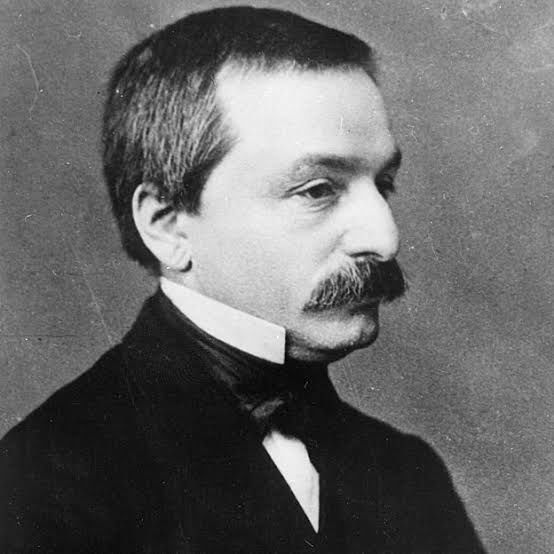
\includegraphics[width=1.0in]{images/kronecker.jpeg}}
\caption*{\small ``God created the integers; all else is the work of man'' -- \href{https://en.wikipedia.org/wiki/Leopold\_Kronecker}{Leopold Kronecker}}
\end{figure}

\begin{figure}[ht]       
\centerline{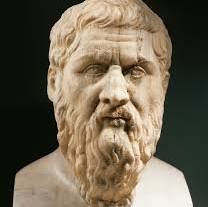
\includegraphics[width=1.0in]{images/plato2.jpeg}}
\caption*{\small ``He is unworthy of the name of man who is ignorant of the fact that the diagonal of a square is incommensurable with its side'' -- \href{https://en.wikipedia.org/wiki/Plato}{Plato}}
\end{figure}
%\epigraph{``God created the integers; all else is the work of man.''}{\textit{Leopold Kronecker (1886)}}



The real numbers are the backbone of modern mathematics. They unify discrete and continuous quantities, allow us to measure lengths, areas, speeds, and forces, and they form the natural domain for calculus, physics, probability, and geometry. Yet the construction of the real numbers is not obvious, and their necessity arises from deep conceptual difficulties that puzzled mathematicians for millennia.

In this chapter we try to build a conceptual and computational foundation for understanding the real numbers, their structure, and the functions defined on them.

\bigskip

%%%%%%%%%%%%%%%%%%%%%%%%%%%%%%%%%%%%%%%%%%%%%%%%%%%%%%%%%%%%%%
\section{Why Do We Need Real Numbers?}

As we saw earlier in these notes, mathematics begins with the natural numbers $\mathbb{N}$,  which suffice for counting and simple arithmetic. But subtraction motivates the integers $\mathbb{Z}$, division motivates the rationals $\mathbb{Q}$, and geometry quickly reveals that even rational numbers are insufficient.  


%\subsection{Why Rational Numbers Are Not Enough}
%
%Examples that push us out of $\mathbb{Q}$:
%
%\begin{itemize}
%\item $\sqrt{2}, \sqrt{3}$ from geometry.
%\item $\pi$ from circle circumference and area.
%\item $e$ from continuous growth.
%\item Infinite decimals such as $0.1010010001\ldots$.
%\end{itemize}
%
%All of these lie outside $\mathbb{Q}$.

\subsection{Incompleteness of the Rationals and the irrational persecution of \href{https://en.wikipedia.org/wiki/Hippasus}{Hippasus}}

In Theorem \ref{thm:sqrt2} we discussed a  classical proof  that shows that $\sqrt{2}\notin \mathbb{Q}$. This was shocking in antiquity and led to the development of more sophisticated number systems. Thus geometry forces us beyond the rationals.

\begin{quote}
``He is unworthy of the name of man who is ignorant of the fact that the diagonal of a square is incommensurable with its side''\quad -- (Plato)
\end{quote}

\href{https://en.wikipedia.org/wiki/Hippasus}{Hippasus} is often credited with the discovery of irrational numbers. According to common folklore the Pythagoreans was rather upset with this discovery, and Hippasus is supposed to have drowned at sea, apparently as a punishment from the gods for divulging this troublesome fact.

There are more reason as to why rational are incomplete. Although $\mathbb{Q}$ is dense on the line, it contains ``holes''. A sequence of rational numbers may converge to a limit that is not rational.

Consider, for example,
\[
y_n = \sum_{k=1}^n 10^{-k!}
\]
Each $y_n$ is rational, but the limit is the Liouville constant, which is not rational.

\begin{theorem}
The \href{https://en.wikipedia.org/wiki/Liouville\_number}{Liouville constant}
\[
L = \sum_{k=1}^{\infty} \frac{1}{10^{k!}}
= \frac{1}{10}+\frac{1}{10^{2}}+\frac{1}{10^{6}}+\frac{1}{10^{24}}+\cdots
\]
is irrational.
\end{theorem}

\begin{proof}
We will use the fact that a decimal number is rational if and only if its decimal expansion is
\emph{eventually periodic}; that is, after some point its digits repeat with a
fixed period. We will prove this in a exercise problem at the end of this chapter.

Let us analyse the decimal expansion of $L$.  The term $\tfrac{1}{10^{k!}}$
contributes a single `1' in the $k!$-th decimal place and zeros elsewhere.
Thus $L$ has a `1' in the decimal positions
\[
1!, \; 2!,\; 3!,\; 4!,\; \dots
\]
and all other digits are $0$.  Therefore the distances between successive
positions of `1' are
\[
\begin{array}{c}
2! -1! = 1  \\
3! - 2! =4 \\
4! - 3! =18 \\
5! -4! =96 \\
\end{array}
\]
and in general

\[
(k+1)! - k! = k!\cdot k
\]


These gaps grow without bound as $k\to\infty$.

Now suppose, for the sake of contradiction, that $L$ is rational.  Then its
decimal expansion would be eventually periodic: there exist integers $N\ge 1$
and $p\ge 1$ such that all digits from position $N$ onward repeat with period
$p$.  In particular, after position $N$, if a digit `1' occurs once, then the
same digit `1' must occur again exactly $p$ places later, and then again $p$
places after that, and so on.  Thus the distances between successive `1's
beyond $N$ must all be \emph{exactly} $p$.

However, choose $k$ large enough that $k!\cdot k > p$ and also $k! > N$.
Then between the `1' at position $k!$ and the next `1' at position $(k+1)!$
there are
\[
(k+1)! - k! = k!\cdot k
\]
zeros --- a gap strictly greater than $p$.  This contradicts the assumption
that the decimal expansion is eventually periodic with period $p$.

Hence no such period $p$ can exist, and the decimal expansion of $L$ is not
eventually periodic.  Therefore $L$ is irrational.
\end{proof}


Hence, rhe rational numbers are not complete. Limits of rational sequences need not be rational. To properly define limits, infinite series, areas, lengths, and solutions of differential equations, we need a larger number system.

\subsection{Zeno's paradox and infinite processes: Achilles and the Tortoise}

\href{https://en.wikipedia.org/wiki/Zeno\_of\_Elea}{Zeno of Elea (5th century BCE)} presented several paradoxes to argue that
motion is impossible.  His most famous example is the paradox of
\emph{Achilles and the Tortoise}, which troubled mathematicians and
philosophers for centuries.  We now explain the paradox in detail and
show how it naturally leads to the concept of limits and infinite series.

\subsubsection*{The Setup}

Suppose Achilles, the fastest of the Greek heroes, runs ten times faster
than a tortoise.  The tortoise is given a head start of $D$ metres.
Common sense says Achilles will quickly overtake the tortoise.  Zeno's
reasoning, however, appeared to show otherwise.

\subsubsection*{Zeno's Argument}

Zeno argued as follows:
\begin{enumerate}
    \item Achilles first runs to the tortoise's starting point (distance $D$).
    \item During that time, the tortoise moves ahead a little.
    \item Achilles then runs to this new position.
    \item Again the tortoise moves slightly ahead.
    \item This continues forever, \emph{ad infinitum}.
\end{enumerate}

Thus Achilles must complete \emph{infinitely many tasks}:
first reach $D$, then $D(1+r)$, then $D(1+r+r^2)$, and so on, where
$r$ is the ratio of the tortoise's speed to Achilles' speed.
Zeno concluded that Achilles can never overtake the tortoise.

\subsubsection*{Mathematical Formulation}

Let $v_A$ be Achilles' speed and $v_T$ be the tortoise's speed, with
$v_A > v_T$.  Let the tortoise's head start be $D$.

The time Achilles takes to reach the tortoise's initial position is
\[
t_1 = \frac{D}{v_A}.
\]
During this time the tortoise moves
\[
D_1 = v_T t_1 = D\cdot \frac{v_T}{v_A}.
\]

Next, Achilles takes
\[
t_2 = \frac{D_1}{v_A} = \frac{D}{v_A}\left(\frac{v_T}{v_A}\right)
\]
to reach that point; during this period the tortoise moves
\[
D_2 = D \left(\frac{v_T}{v_A}\right)^2.
\]

Continuing, we obtain an infinite sequence of positive times
\[
t_1, \; t_2, \; t_3,\; \dots
\]
with
\[
t_n = \frac{D}{v_A}\left(\frac{v_T}{v_A}\right)^{n-1}.
\]

Thus the total time required for Achilles to reach all points previously
occupied by the tortoise is
\[
T = t_1 + t_2 + t_3 + \cdots
 = \frac{D}{v_A}
   \left(1 + r + r^2 + r^3 + \cdots\right),
\]
where
\[
r = \frac{v_T}{v_A} \quad \text{and} \quad 0 < r < 1.
\]

\subsubsection*{Resolution via convergent geometric series}

We will show in Section \ref{sec:apgp} that the  infinite geometric series with $0 < r < 1$ satisfies
\[
1 + r + r^2 + r^3 + \cdots = \frac{1}{1-r}.
\]

Hence
\[
T
 = \frac{D}{v_A}\cdot \frac{1}{1-r}
 = \frac{D}{v_A - v_T}.
\]

That is, the infinite sum actually converges to a finite quantity, a rational number if $r$ is rational. This is the standard ``relative speed'' formula for the time taken for a
faster runner to catch a slower one.  The total time $T$ is finite.

\emph{Achilles does indeed overtake the tortoise.}

\subsubsection*{What Zeno misunderstood}

Zeno implicitly assumed that a process involving infinitely many steps
must take an infinite amount of time.  Modern mathematics shows that
an infinite series of positive quantities may converge to a finite sum.
Here the quantities $t_n$ become smaller so rapidly that their infinite
sum remains finite.

This is only made rigorous in the \emph{real numbers}, which allow us to
define limits and convergent series.  In this sense, Zeno's paradox
hints at the need for a complete number system.


%Bertrand Russell famously observed:
%\begin{quote}
%``Zeno's arguments were designed to bring out contradictions implicit
%in the ordinary ideas of space and time.''
%\end{quote}

\begin{figure}[ht]       
\centerline{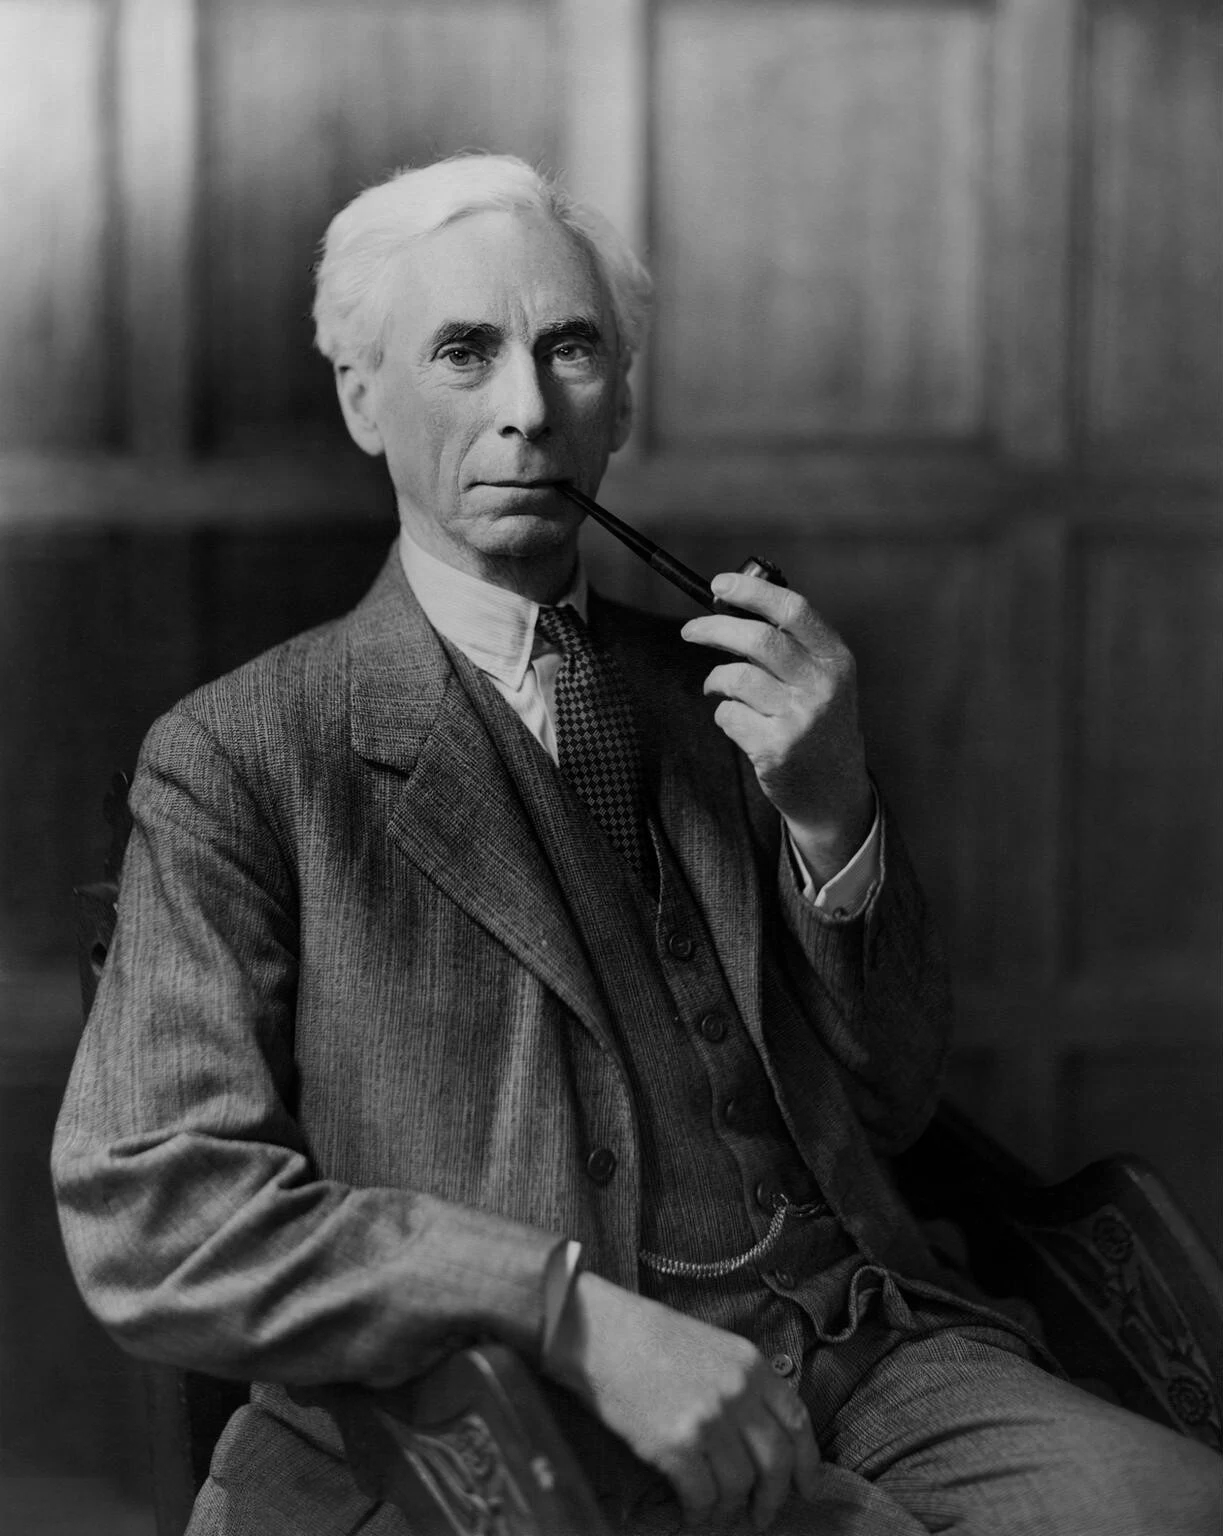
\includegraphics[width=1.0in]{images/russel2.jpg}}
\caption*{\small ``The paradoxes of Zeno the Eleatic and the difficulties in the analysis of space, 
of time, and of motion, are all completely explained by means of the modern 
theory of continuity. This is because a non-contradictory theory has been 
found, according to which the continuum is composed of an infinity of distinct 
elements; and this formerly appeared impossible'' --  \href{https://en.wikipedia.org/wiki/Bertrand_Russell}{Bertrand Russell}}
\end{figure}
\begin{figure}[ht]       
\centerline{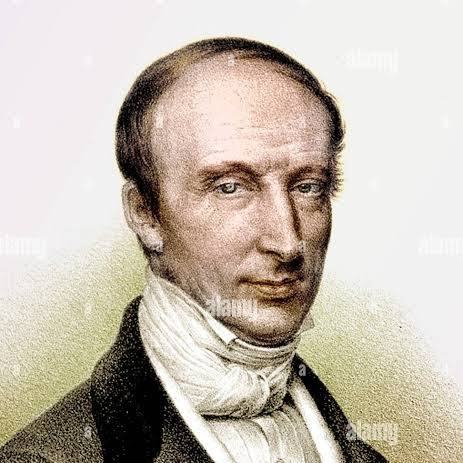
\includegraphics[width=1.0in]{images/cauchy.jpg}}
\caption*{\small ``It is by the idea of limit alone that the calculus becomes a rigorous science.'' --  \href{https://en.wikipedia.org/wiki/Augustin-Louis_Cauchy}{A.–L. Cauchy}, Cours d’Analyse (1821)}
\end{figure}
\begin{figure}[ht]       
\centerline{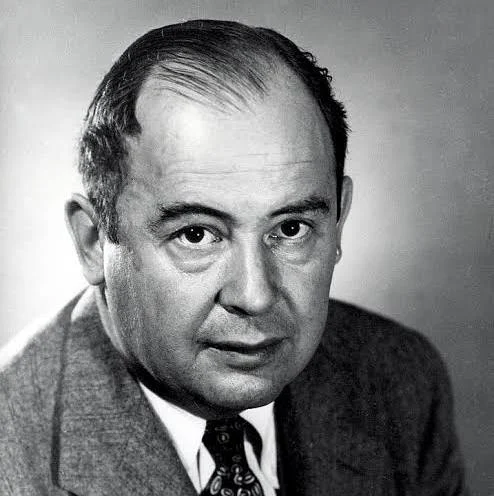
\includegraphics[width=1.0in]{images/vonneumann.png}}
\caption*{\small ``The calculus was the first achievement of modern mathematics and it is difficult to overestimate its importance. I think it defines more unequivocally than anything else the inception of modern mathematics; and the system of mathematical analysis, which is its logical development, still constitutes the greatest technical advance in exact thinking.'' --  \href{https://en.wikipedia.org/wiki/John_von_Neumann}{John von Neumann}}
\end{figure}


Understanding the resolution of Zeno's paradox requires understanding limits, convergence, and the structure of the real numbers. 
The resolution uses \emph{infinite series} and the idea of a \emph{limit}. These require a complete number system --- the real numbers. A follow up course on \emph{Calculus} is strongly recommended.

\section{The Real Line as a Continuum}

One way to view the real line is as the set of all (possibly infinite, non-repeating) decimals. Another is to view the real line as the completion of the rationals under limits of Cauchy sequences.

\begin{definition}[Cauchy Sequence]
A sequence $(x_n)$ of real or rational numbers is called a \emph{Cauchy
sequence} if for every $\varepsilon>0$ there exists $N\in\mathbb{N}$
such that for all $m,n\ge N$,
\[
|x_m - x_n| < \varepsilon.
\]
\end{definition}

In other words, the terms of the sequence eventually become arbitrarily
close to one another.  It turns out that every Cauchy sequence converges in $\mathbb{R}$,
but not necessarily in $\mathbb{Q}$, which shows that the rationals are
not complete.


\subsection{Cantor: The Reals are uncountable}

\begin{figure}[ht]       
\centerline{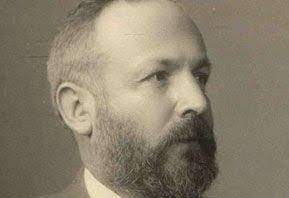
\includegraphics[width=1.0in]{images/cantor2.jpeg}}
\caption*{\small ``I see it, but I don't believe it!'' -- \href{https://en.wikipedia.org/wiki/Georg_Cantor}{Georg Cantor}}
\end{figure}

In 1874, Cantor used his celebrated \emph{diagonal argument} to prove that no list can contain all real numbers in $(0,1)$.

\begin{theorem}[Cantor's Diagonal Argument]
The interval $(0,1)$ is uncountable.  In particular, there is no bijection
between the natural numbers $\mathbb{N}$ and the real numbers in $(0,1)$.
\end{theorem}

\begin{proof}
Suppose, for the sake of contradiction, that $(0,1)$ is countable.
Then every real number in $(0,1)$ has a decimal expansion of the form
\[
0.a_1 a_2 a_3 \dots,
\]
and our assumption implies that it is possible to list \emph{all} such
numbers in a single infinite sequence.  Thus suppose we have an
enumeration
\[
x_1, x_2, x_3, \ldots
\]
of all real numbers in $(0,1)$, where each $x_n$ is written in decimal
form as
\[
\begin{array}{ccc}
x_1 & = & 0.a_{11} a_{12} a_{13} a_{14} \dots \\
x_2 & = & 0.a_{21} a_{22} a_{23} a_{24} \dots \\
       & \vdots & \\
x_n & = & 0.a_{n1} a_{n2} a_{n3} a_{n4} \dots \\
  & \vdots & \\
\end{array}
\]
Here $a_{nk} \in \{0,1,2,\dots,9\}$ is the $k$-th digit of the $n$-th
number in the list.

\medskip
\noindent\emph{Important convention.}  
To avoid the ambiguity of decimal expansions such as
$0.2499999\ldots = 0.25$, we assume that no number in the list ends in
an infinite tail of $9$'s.  Every real number in $(0,1)$ has at least one
representation without trailing $9$'s, so this assumption does not omit
any real number.

\medskip
Now we construct a new number $y$ whose decimal digits differ from
the diagonal digits of the list.  Define
$y = 0.b_1 b_2 b_3 \dots$ by
\[
b_k =
\begin{cases}
5, &\text{if } a_{kk} \neq 5,\\[4pt]
4, &\text{if } a_{kk} = 5.
\end{cases}
\]
In other words, $b_k$ is chosen so that it \emph{differs} from $a_{kk}$.
This is always possible because there are ten possible digits, and we
deliberately avoid choosing the digit $9$, so $y$ will not end in an
infinite string of $9$'s.

\medskip
Consider any index $n\in\mathbb{N}$.  We compare $y$ with the $n$-th
number $x_n$ in the list.  The $n$-th digit of $x_n$ is $a_{nn}$, while
the $n$-th digit of $y$ is $b_n$, which was chosen to be \emph{different}
from $a_{nn}$.  Therefore,
\[
y \neq x_n.
\]

Since this argument holds for every $n$, we conclude that the constructed
number $y$ is different from $x_n$ for all $n\in\mathbb{N}$.  But this
contradicts our assumption that $(0,1)$ was completely enumerated by the
sequence $x_1, x_2, x_3, \dots$.

\medskip
Thus our original assumption was false.  No such complete enumeration
exists, and therefore $(0,1)$ is uncountable.
\end{proof}

\begin{figure}[ht]       
\centerline{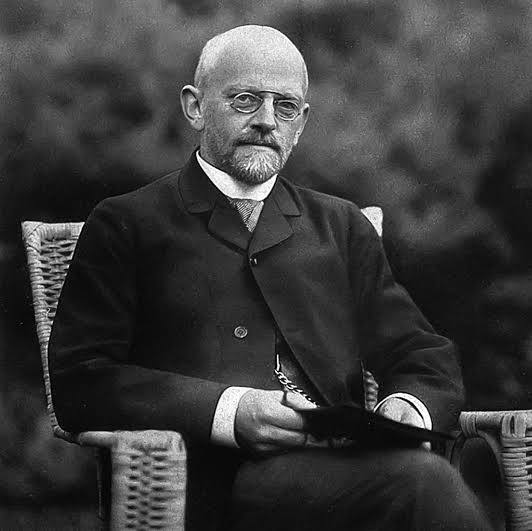
\includegraphics[width=1.0in]{images/hilbert.jpeg}}
\caption*{\small ``No one shall expel us from the paradise that Cantor has created.'' --  \href{https://en.wikipedia.org/wiki/David_Hilbert}{David Hilbert}}
\end{figure}

The result was revolutionary and laid the foundations of modern set theory. Quite amazingly, \emph{diagonalization} as a  proof technique has also turned out to be foundational in logic and computer science.

%%%%%%%%%%%%%%%%%%%%%%%%%%%%%%%%%%%%%%%%%%%%%%%%%%%%%%%%%%%%%%
\section{Algebraic and Transcendental Numbers}
\label{sec:algebraicnumbers}
The irrationals split into two classes.

A real number $x$ is \emph{algebraic} if it is a root of (a solution of) an equation like
\[
a_n x^n + a_{n-1}x^{n-1} + \cdots + a_1 x + a_0 = 0
\]
with rational coefficients $a_0, a_1,\dots,a_n$. Expressions such as the left hand side of the above equation are called \emph{polynomials} and the solutions are called its \emph{roots}.

Some examples are
\[
\sqrt{2},\qquad \sqrt[3]{5},\qquad \frac{1+\sqrt{5}}{2}
\]

If a number is not algebraic, it is \emph{transcendental}.  
Some famous examples are $e$ and $\pi$ which will soon discuss.


\href{https://en.wikipedia.org/wiki/Liouville\_number}{Liouville (1844)} constructed numbers that are ``too well approximated'' by rationals:
\[
L = \sum_{k=1}^\infty 10^{-k!}
\]
Liouville proved that $L$ is transcendental.

\begin{quote}
``Transcendental numbers are not rare; they are, in fact, the rule.''  
\textit{--- \href{https://en.wikipedia.org/wiki/Kurt_Mahler}{Kurt Mahler}}
\end{quote}

%%%%%%%%%%%%%%%%%%%%%%%%%%%%%%%%%%%%%%%%%%%%%%%%%%%%%%%%%%%%%%
\subsection{How fast do our money grow? Simple and compound interests}

When we invest  in a financial instrument our money earns \emph{interest} and grows.

\emph{Simple interest}
assumes that interest is calculated only on the original principal, and
that previously earned interest does not itself earn further interest.

Let
\[
P = \text{principal (initial amount)}, \qquad
r = \text{annual interest rate}, \qquad
t = \text{time in years}.
\]
Under simple interest, the total amount after $t$ years is
\[
A(t) = P(1 + rt).
\]

This is a linear function of $t$.  The amount increases at a constant
rate $Pr$ per year, so the graph of $A(t)$ against $t$ is a straight line.

\begin{example}
Suppose you invest
\[
P = \mbox{\rupee}10{,}000 
\]
at an annual simple interest rate of $r = 0.08$ (i.e.\ 8\% per year). Then

\vspace{0.25in}
\begin{tabular}{ll}
\hline
After 1 year: &  $A(1) = 10000(1 + 0.08) = 10800$ \\
After 3 years: &  $A(3) = 10000(1 + 0.08\times 3) = 10000(1 + 0.24) = 12400$ \\
After 10 years: & $A(10) = 10000(1 + 0.08\times 10)  = 10000(1 + 0.80) = 18000$ \\
\hline
\end{tabular}
\vspace{0.25in}

In each year, the amount increases by the same amount:
\[
Pr = 10000\times 0.08 = \mbox{\rupee} 800 
\]
\end{example}


Under \emph{compound interest}, interest is added periodically and in each period
the previously earned interest itself earns further interest.  If $P$ is
the principal, $r$ is the annual interest rate, and interest is compounded
once per year, then the amount after $t$ years is
\[
A_c(t) = P(1+r)^{t}.
\]

\begin{example}
For the same values as in the simple–interest example,
\[
P = 10{,}000,\qquad r = 0.08,
\]
we obtain
\[
A_c(t)=10000(1.08)^t
\]
Thus,

\vspace{0.25in}
\begin{tabular}{ll}
\hline
After 1 year: &  $A(1) = 10000(1.08) = 10800$ \\
After 3 years: &  $A(3) = 10000(1.08)^3 = 12597.12 $ \\
After 10 years: & $A(10) = 10000(1.08)^10  = 21589.25$ \\
\hline
\end{tabular}
\vspace{0.25in}

\end{example}

While simple interest grows linearly, compound interest grows
exponentially.  Over long durations the difference becomes significant, 
and compounded growth eventually ``pulls away'' from linear
growth.

\begin{figure}[h]
\centering
\resizebox{0.7\textwidth}{!}{%
\begin{tikzpicture}[scale=0.85]

% ----- Axes -----
\draw[->] (0,0) -- (21,0) node[right] {Time $t$ (years)};
\draw[->] (0,0) -- (0,8) node[above] {Amount (rupees)};

% y-axis ticks (scaled: +5000 rupees = +1 unit)
\foreach \y/\lab in {0/10, 1/15, 2/20, 3/25, 4/30, 5/35, 6/40, 7/45, 8/50} {
    \draw (-0.15,\y) -- (0.15,\y);
    \node[left] at (-0.25,\y) {\lab,000};
}

% x-axis ticks
\foreach \x in {0,5,10,15,20} {
    \draw (\x,0) -- (\x,-0.15);
    \node[below] at (\x,-0.2) {\x};
}

% ----- Simple interest: y=0.16 t -----
\draw[thick] (0,0) -- (20,3.2);
\foreach \t/\y in {0/0, 5/0.8, 10/1.6, 15/2.4, 20/3.2} {
    \fill (\t,\y) circle (2pt);
}

% ----- Compound interest: annual -----
% Precomputed values:
% t=0: 10000       -> y=0
% t=5: 14693.28    -> y=0.938656
% t=10: 21589.25   -> y=2.31785
% t=15: 31721.64   -> y=4.34433
% t=20: 46517.34   -> y=7.30347

\draw[thick, dashed]
    plot[smooth] coordinates {
        (0,0)
        (5,0.938656)
        (10,2.31785)
        (15,4.34433)
        (20,7.30347)
    };

\foreach \t/\y in {0/0, 5/0.938656, 10/2.31785, 15/4.34433, 20/7.30347} {
    \fill (\t,\y) rectangle ++(0.12,0.12);
}

% ----- Legend -----
\begin{scope}[shift={(12,7.2)}]
    \draw[thick] (0,0) -- (1,0);
    \node[right] at (1.2,0) {Simple interest};

    \draw[thick, dashed] (0,-0.7) -- (1,-0.7);
    \node[right] at (1.2,-0.7) {Compound interest};
\end{scope}

\end{tikzpicture}%
}
\caption{Simple vs annually compounded growth at $8\%$ for $P=10{,}000$ over 20 years.
Vertical scale: $y=(A(t)-10000)/5000$.}
\end{figure}

As $n$ increases, this expression approaches the continuously compounded
growth
\[
A(t) = Pe^{rt},
\]
revealing the natural appearance of the constant $e$.  Thus the transition
from simple to compound interest provides a natural pathway from linear
to exponential growth.

\subsection{From compound interest to the number \texorpdfstring{$e$}{e}}

Compound interest provides a natural setting in which the exponential
number $e$ appears.  Suppose a principal amount $P$ is invested at an
annual interest rate $r$, but interest is now credited not once a year,
but $n$ times per year.  In each compounding period the interest rate is
$r/n$, so the amount after one year becomes
\[
A_n(1) = P\left(1 + \frac{r}{n}\right)^{n}.
\]

For example:
\begin{itemize}
    \item with $n=1$ (annual compounding), we obtain $P(1+r)$,
    \item with $n=4$ (quarterly compounding), we obtain
    $P\left(1+\frac{r}{4}\right)^4$,
    \item with $n=12$ (monthly compounding), we obtain
    $P\left(1+\frac{r}{12}\right)^{12}$,
    \item with $n=365$ (daily compounding), we obtain
    $P\left(1+\frac{r}{365}\right)^{365}$.
\end{itemize}

As $n$ increases, interest is credited more and more frequently, and the
amount grows slightly larger.  A natural mathematical question is:
\[
\textit{What happens as } n \to \infty?
\]

\medskip
\noindent
To study this limit, let us first focus on the core expression
\[
\left(1 + \frac{1}{n}\right)^{n}.
\]
One can check numerically that
\[
\left(1+\frac{1}{n}\right)^n
=
2.0000,\; 2.2500,\; 2.3707,\; 2.3979,\; 2.7048,\;\dots
\]
for $n=1,2,3,4,10,\dots$, and that the sequence increases and approaches
a limiting value.  This limit is denoted by the symbol $e$\footnote{Estimating its value will require some advanced techniques which an interested reader may look up.}.
\[
e = \lim_{n\to\infty}\left(1+\frac{1}{n}\right)^{n} \approx  2.71828
\]

The limit can also be written as an infinite sum. The full Binomial expansion becomes
\[
\left(1+\frac{1}{n}\right)^{n}
=
1
+ 1
+ \frac{1}{2}\left(1-\frac{1}{n}\right)
+ \frac{1}{6}\left(1-\frac{1}{n}\right)\left(1-\frac{2}{n}\right)
+ \cdots.
\]

As $n\to\infty$, $\frac{1}{n}\to 0$, Hence,
\[
e = 1 + 1 + \frac{1}{2!} +  \frac{1}{3!} +  \frac{1}{4!} + \cdots
\]

\vspace{0.25in}
Thus, continuous compounding at rate $r$ leads to the amount
\[
A(1)=Pe^{\,r}
\]

\noindent
In general, after $t$ years the continuously compounded amount becomes\footnote{\href{https://en.wikipedia.org/wiki/Jacob_Bernoulli}{Jacob Bernoulli} discovered this limit while studying compound interest in 1683. \href{https://en.wikipedia.org/wiki/Leonhard_Euler}{Leonhard Euler} later linked it to calculus and defined it analytically.}
\[
A(t)=Pe^{\,rt}.
\]
This is the fundamental exponential-growth formula.  The appearance of
$e$ is therefore not mysterious: it arises naturally as the limiting
value of compound interest when interest is credited infinitely often.

\begin{quote}
\emph{``The number $e$ is the unique real number for which continuous
growth at rate 1 yields a unit increase in one time unit.''}
\end{quote}

This interpretation makes $e$ one of the most important constants in
mathematics, appearing in finance, probability theory, calculus,
differential equations, and many dynamical processes in the natural and
social sciences.

%%%%%%%%%%%%%%%%%%%%%%%%%%%%%%%%%%%%%%%%%%%%%%%%%%%%%%%%%%%%%%
\subsection{The Number $\pi$ from Geometry}

All circles are similar: any circle can be obtained from any other by a
uniform scaling.  Under scaling by a factor $k>0$, every length is multiplied
by $k$.  Hence circumference and diameter scale by the same factor, so their
ratio is unchanged.

\begin{figure}[h]
\centering
\begin{tikzpicture}[scale=1]

% Small circle
\draw[thick] (-3,0) circle (1.2);
\fill (-3,0) circle (1pt);
\node at (-3,-1.7) {$\text{Circle of radius } r$};

% Radius arrow small
\draw[->] (-3,0) -- (-1.8,0) node[midway, above] {$r$};

% Diameter arrow small
\draw[<->] (-4.2,0) -- (-1.8,0) node[midway, below] {$D=2r$};

% label circumference
\node at (-3,1.55) {$C$};

% Big circle (scaled)
\draw[thick] (3,0) circle (2.2);
\fill (3,0) circle (1pt);
\node at (3,-2.7) {$\text{Circle of radius } kr$};

% Radius arrow big
\draw[->] (3,0) -- (5.2,0) node[midway, above] {$kr$};

% Diameter arrow big
\draw[<->] (0.8,0) -- (5.2,0) node[midway, below] {$D'=2kr=kD$};

% label circumference
\node at (3,2.55) {$C'$};

% Scaling arrow between circles
\draw[->, thick] (-0.4,1.8) -- (0.4,1.8);
\node at (0,2.1) {scale by $k$};

% Text below to emphasize ratio
\node[align=center] at (0,-4.0)
{$C' = kC,\quad D' = kD\quad\Rightarrow\quad \dfrac{C'}{D'}=\dfrac{C}{D}.$};

\end{tikzpicture}
\caption{Scaling a circle by factor $k$ multiplies both circumference and
diameter by $k$, so the ratio $C/D$ is the same for all circles.}
\end{figure}
\begin{definition}
For every circle,
\[
\pi = \frac{C}{D} = \frac{C}{2r}.
\]
\end{definition}

For a disk of radius $r$, the area is given as
\[
A(r) = \pi r^2.
\]

Thus $\pi = A(1)$: the area of the unit disk.

\subsubsection{Approximations of $\pi$}

\href{https://en.wikipedia.org/wiki/Archimedes}{Archimedes} approximated $\pi$ using inscribed and circumscribed $n$-gons. Using a $96$-gon, he showed
\[
3\frac{10}{71} < \pi < 3\frac{1}{7}.
\]

The \href{https://en.wikipedia.org/wiki/Leibniz_formula_for_\%CF\%80}{Leibniz formula for $\pi$} obtained using a geometric series approximation and integration is given as
\[
\frac{\pi}{4} = 1 - \frac13 + \frac15 - \frac17 + \cdots
\]
This series converges slowly but gives an exact expression.  This series is also sometimes called the Madhava-Leibniz series as it was first discovered by \href{https://en.wikipedia.org/wiki/Madhava_of_Sangamagrama}{Madhava of Sangamagrama}\footnote{See \href{https://en.wikipedia.org/wiki/Approximations_of_\%CF\%80}{https://en.wikipedia.org/wiki/Approximations\_of\_$\pi$} for a history of various approximations of $\pi$.}. It can be shown that $\pi$ is a transcendental number.


\section*{Problems}

\begin{enumerate}

\item (\textbf{Incompleteness of the rationals})
Give an example of a Cauchy sequence of rational numbers that does \emph{not} converge
to any rational number. Explain why this demonstrates a “gap’’ in $\mathbb{Q}$.

\item (\textbf{Achilles and the Tortoise})
In the Achilles–Tortoise setup where Achilles runs at twice the speed of the tortoise,
write the explicit geometric series representing Achilles’ motion.  
Compute its sum and argue why the paradox dissolves once infinite sums are allowed.

\item (\textbf{Density})
Prove that between any two irrational numbers there exists a rational number.
(Hint: scale and shift.)

\item (\textbf{Decimal expansions})
Give an example of a non-terminating repeating decimal and a non-repeating decimal.
Classify each as rational or irrational and justify your answer.

\item (\textbf{Cantor’s diagonal argument})
Explain why the diagonal method does not contradict the fact that decimal
representations have non-uniqueness (e.g.\ $0.4999\ldots = 0.5$).
Why does the argument still go through?

\item (\textbf{Countability vs uncountability})
Show that the set of all infinite binary sequences is uncountable
by giving a diagonal proof analogous to Cantor’s proof for $(0,1)$.

\item (\textbf{Algebraic vs transcendental})
Prove that the number
\[
L = \sum_{k=1}^\infty 10^{-k!}
\]
is irrational.  
(Hint: compare $L$ with rational numbers truncated after $n!$ decimal places.)

\item (\textbf{From compound interest to $e$})
Compute $\left(1+\frac{1}{n}\right)^{n}$ for $n=1,2,5,10,100,1000$.
Does the sequence appear to converge?
How does this motivate the definition of $e$?

\item (\textbf{$e$ as a limit})
Show that the sequence
\[
a_n = \left(1+\frac{1}{n}\right)^{n+1}
\]
is bounded above by $e$.  
(Hint: use monotonicity and the binomial expansion.)

\item (\textbf{Archimedes' method})
Using a circumscribed $n$-gon around a unit circle, derive an upper bound on $\pi$.
Compute the bound explicitly for $n=6$ and $n=12$.

\item (\textbf{Transcendentals exist “in abundance’’})
Show that the set of algebraic numbers is countable.
Conclude that “almost all’’ real numbers are transcendental.

\end{enumerate}

\chapter{The Real Toolkit: Sequences, Functions, and Equations}

\begin{figure}[ht]       
\centerline{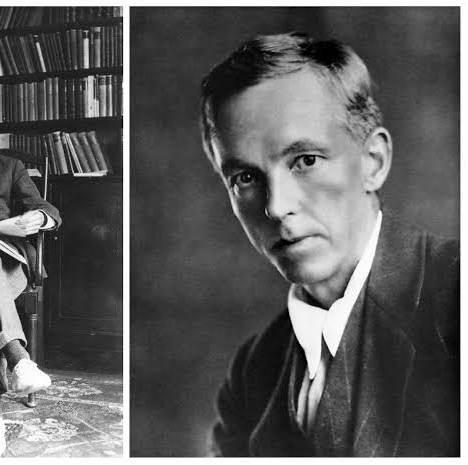
\includegraphics[width=1.0in]{images/hardy2.jpeg}}
\caption*{\small ``A mathematician, like a painter or a poet, is a maker of patterns'' -- \href{https://en.wikipedia.org/wiki/G._H._Hardy}{G. H. Hardy}}
\end{figure}

%\begin{figure}[ht]       
%\centerline{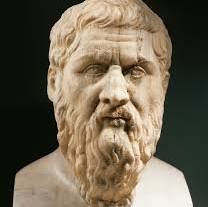
\includegraphics[width=1.0in]{images/plato2.jpeg}}
%\caption*{\small ``He is unworthy of the name of man who is ignorant of the fact that the diagonal of a square is incommensurable with its side'' -- \href{https://en.wikipedia.org/wiki/Plato}{Plato}}
%\end{figure}

The real numbers are more than a continuum filling the gaps left by the rationals—they form a versatile algebraic toolkit for describing change, predicting patterns, and solving practical problems. In this chapter we develop the basic algebra of the reals as it appears in everyday mathematical modelling: from  arithmetic and geometric progressions; from polynomials and their remarkable power of unique interpolation to the curve-fitting techniques that underlie modern data analysis; and from real-valued functions to systems of linear equations that allow us to solve for unknowns in structured ways. Together, these ideas illustrate how the algebra of the real numbers becomes a unifying language for patterns, growth, and relationships in both mathematics and the world around us.

%%%%%%%%%%%%%%%%%%%%%%%%%%%%%%%%%%%%%%%%%%%%%%%%%%%%%%%%%%%%%%
\section{Arithmetic and geometric progressions}
\label{sec:apgp}

Arithmetic and geometric progressions are two of the simplest infinite families
of sequences, and they sit at the gateway between discrete sums and the
idea of limits.  They also provide the first nontrivial examples of
closed-form formulas for sums.

\subsection{Arithmetic progressions (AP)}

\begin{definition}
A sequence $(a_n)$ is an \emph{arithmetic progression} if the difference between
consecutive terms is constant.  That is, there exists a real number $d$
such that
\[
a_{n+1}-a_n=d\quad\text{for all }n\ge 1.
\]
The number $d$ is called the \emph{common difference}.
\end{definition}

Hence an AP has the form
\[
a,\ a+d,\ a+2d,\ \dots,\ a+(n-1)d,\ \dots
\]
and the $n$-th term is
\[
a_n=a+(n-1)d.
\]

\subsubsection*{Sum of the first $n$ terms: a double-counting derivation}

Let
\[
S_n = a + (a+d) + (a+2d) + \cdots + (a+(n-1)d)
\]
be the sum of the first $n$ terms.

Write the same sum in reverse order:
\[
S_n = (a+(n-1)d) + (a+(n-2)d) + \cdots + (a+d) + a.
\]

Now add these two expressions term-by-term.  Each pair adds to the same value\footnote{This ``pairing'' trick is often attributed to the young \href{https://en.wikipedia.org/wiki/Carl_Friedrich_Gauss}{Gauss}, who is said
to have summed $1+2+\cdots+100$ instantly by noticing that $1+100=2+99=\cdots=101$.}:
\[
\bigl(a+(k-1)d\bigr) + \bigl(a+(n-k)d\bigr)=2a+(n-1)d.
\]
There are $n$ such pairs, so
\[
2S_n = n\bigl(2a+(n-1)d\bigr).
\]
Therefore,
\[
\boxed{\displaystyle
S_n = \frac{n}{2}\bigl(2a+(n-1)d\bigr)
     = \frac{n}{2}\,(a_1+a_n).
}
\]

\begin{example}[Sum of the first $n$ natural numbers]
Here $a=1$ and $d=1$, so
\[
S_n=\frac{n}{2}(2+(n-1))=\frac{n(n+1)}{2}.
\]
\end{example}

\begin{example}[Sum of the first $n$ odd numbers]
The odd numbers form an AP:
\[
1,3,5,\dots,(2n-1),
\]
with $a=1$, $d=2$. Thus
\[
S_n=\frac{n}{2}\bigl(2\cdot 1+(n-1)\cdot 2\bigr)
=\frac{n}{2}(2n)=n^2.
\]
So the sum of the first $n$ odd numbers is $n^2$.
\end{example}

\subsection{Geometric progressions (GP)}

\begin{definition}
A sequence $(g_n)$ is a \emph{geometric progression} if the ratio between
consecutive terms is constant.  That is, there exists a real number $r$
such that
\[
\frac{g_{n+1}}{g_n}=r\quad\text{for all }n\ge 1,
\]
provided $g_n\neq 0$.
The number $r$ is called the \emph{common ratio}.
\end{definition}

A GP has the form
\[
a,\ ar,\ ar^2,\ \dots,\ ar^{n-1},\ \dots
\]
and the $n$-th term is
\[
g_n=ar^{n-1}.
\]

\subsubsection*{Sum of the first $n$ terms}

Let
\[
S_n = a + ar + ar^2 + \cdots + ar^{n-1}.
\]
Multiply both sides by $r$:
\[
rS_n = ar + ar^2 + \cdots + ar^{n}.
\]
Subtract:
\[
S_n - rS_n = a - ar^{n}.
\]
Hence
\[
(1-r)S_n = a(1-r^n),
\]
and therefore, if $r\neq 1$,
\[
\boxed{\displaystyle
S_n = a\,\frac{1-r^{n}}{1-r}.
}
\]
When $r=1$, the GP is constant and $S_n=na$.

\subsubsection*{Infinite geometric series}

If $|r|<1$, then $r^n\to 0$ as $n\to\infty$, so
\[
S_\infty
=\lim_{n\to\infty} S_n
=\lim_{n\to\infty} a\,\frac{1-r^n}{1-r}
=\frac{a}{1-r}.
\]
Thus
\[
\boxed{\displaystyle
a+ar+ar^2+\cdots = \frac{a}{1-r}\quad (|r|<1).
}
\]

This is one of the earliest places where limits naturally enter: an infinite
sum makes sense only because the partial sums converge.


\begin{example}[Zeno's geometric series]
\[
\frac12+\frac14+\frac18+\cdots
\]
is a GP with $a=\tfrac12$ and $r=\tfrac12$, so
\[
S_\infty = \frac{1/2}{1-1/2}=1.
\]
This is exactly the mathematical resolution of Zeno’s paradox.
\end{example}

\begin{example}[A repeating decimal as a GP]
\[
0.\overline{3}=0.3+0.03+0.003+\cdots
\]
is a GP with $a=0.3$ and $r=0.1$. Hence
\[
0.\overline{3} = \frac{0.3}{1-0.1}=\frac{0.3}{0.9}=\frac13.
\]
\end{example}

\subsection*{Remarks}

\begin{itemize}
    \item AP sums grow \emph{quadratically} in $n$ when $d\neq 0$,
          reflecting linear increments.
    \item GP sums grow \emph{exponentially} in $n$ when $|r|>1$,
          reflecting multiplicative change.
    \item The infinite GP formula is the first rigorous example of
          a convergent infinite series, and is a key bridge to calculus.
\end{itemize}

\section{Polynomials}

Polynomials are among the most fundamental objects in algebra.  They form
a rich class of functions that are easy to compute with, easy to
approximate, and powerful enough to model a wide variety of phenomena.
In this section we introduce the basic theory of polynomials, discuss the
unique interpolation theorem, and show how polynomials naturally arise in
curve fitting and other applications.

\subsection{Definition and degree}

A \emph{polynomial} over the real numbers is a function of the form
\[
P(x) = a_0 + a_1 x + a_2 x^2 + \cdots + a_n x^n,
\]
where $a_0,a_1,\dots,a_n\in\mathbb{R}$ and $n$ is a nonnegative integer.
The number $n$ is the \emph{degree} of the polynomial (provided $a_n\neq 0$).

\begin{itemize}
    \item A polynomial of degree $0$ is a constant function.
    \item A polynomial of degree $1$ is a linear function. It gives the equation of a straight line.
    \item A polynomial of degree $2$ is a quadratic function.
    \item A polynomial of degree $3$ is a cubic function, and so on.
\end{itemize}

The set of all polynomials with real coefficients is denoted by
$\mathbb{R}[x]$.  Polynomials are defined everywhere on $\mathbb{R}$.  They also satisfy the useful property that if
\[
P(x)=0\quad\text{for infinitely many distinct }x\in\mathbb{R},
\]
then $P$ must be the zero polynomial.  This is called the
\emph{identity theorem for polynomials}.

\subsection{Basic algebraic properties}

Polynomials can be added and multiplied term-by-term, following the same
rules as with ordinary algebraic expressions.  Here we illustrate both
operations with simple examples.

\[
\deg(P+Q)\le\max(\deg P,\deg Q),\qquad
\deg(PQ)=\deg P+\deg Q,
\]
unless cancellation occurs in the leading terms.

\subsubsection*{Polynomial addition}

Let
\[
P(x)=3x^3 - 2x + 5,\qquad
Q(x)=4x^2 + x - 1.
\]
To compute $P(x)+Q(x)$, we combine like terms:
\[
\begin{aligned}
P(x)+Q(x)
&= (3x^3) + (4x^2) + (-2x+x) + (5-1) \\
&= 3x^3 + 4x^2 - x + 4.
\end{aligned}
\]
Thus
\[
\boxed{\,P(x)+Q(x)=3x^3 + 4x^2 - x + 4.\,}
\]

\subsubsection*{Polynomial multiplication}

Let
\[
A(x)=2x^2 - 3x + 1,\qquad
B(x)=x - 4.
\]
Multiplying out (using distributivity):
\[
\begin{aligned}
A(x)B(x)
&=(2x^2)(x) + (2x^2)(-4)
 +(-3x)(x)+(-3x)(-4)
 +(1)(x)+(1)(-4) \\
&= 2x^3 - 8x^2 - 3x^2 + 12x + x -4.
\end{aligned}
\]
Now combine like terms:
\[
\begin{aligned}
A(x)B(x)
&= 2x^3 - 11x^2 + 13x - 4.
\end{aligned}
\]
So
\[
\boxed{\,A(x)B(x)=2x^3 - 11x^2 + 13x - 4.\,}
\]

\subsection{The decimal system as a polynomial representation}

Every finite decimal expansion
\[
d_k d_{k-1} \cdots d_1 d_0
\]
represents a number that can be interpreted as a polynomial in~$10$:
\[
d_k 10^{k} + d_{k-1} 10^{k-1} + \cdots + d_1 10 + d_0.
\]
In this sense, the decimal numeral system is simply a \emph{polynomial in the base~$10$}.

\begin{example}
\begin{enumerate}
\item A whole number:
\[
374 = 3\cdot 10^2 + 7\cdot 10^1 + 4\cdot 10^0.
\]
\item A larger number:
\[
5{,}182
= 5\cdot 10^3 + 1\cdot 10^2 + 8\cdot 10 + 2.
\]
\item A decimal (fractional) number:
For digits after the decimal point, we use negative powers of~10:
\[
46.327
= 4\cdot 10^1
+ 6\cdot 10^0
+ 3\cdot 10^{-1}
+ 2\cdot 10^{-2}
+ 7\cdot 10^{-3}.
\]
\end{enumerate}
\end{example}
\medskip

Thus every decimal numeral is nothing more than a polynomial expression
in the base~$10$ with coefficients drawn from $\{0,1,\dots,9\}$.
This viewpoint is fundamental in computer science (base~2),
engineering (base~16), and number theory (general base-$b$ expansions).

\begin{exercise}
Explain the junior school algorithm for integer multiplication in terms of polynomial multiplications. Explain how is this repeated addition?
\end{exercise}

\subsection{The unique interpolation theorem}

One of the most remarkable facts about polynomials is that they can be
used to fit any finite collection of data points with a unique polynomial
of sufficiently small degree.

\begin{theorem}[Unique Interpolating Polynomial]
Let $(x_0,y_0), (x_1,y_1), \dots, (x_n,y_n)$ be $n\!+\!1$ data points with
\[
x_i \neq x_j \quad \text{whenever } i\neq j.
\]
Then there exists a polynomial $P(x)$ of degree at most $n$ such that
\[
P(x_i)=y_i \quad \text{for all } i=0,1,\dots,n,
\]
and this polynomial is unique.
\end{theorem}

\begin{proof}
We prove existence and uniqueness.

\subsubsection*{Existence (\href{https://en.wikipedia.org/wiki/Joseph-Louis_Lagrange}{Lagrange} construction)}
For each $k\in\{0,1,\dots,n\}$ define the \emph{Lagrange basis polynomial}
\[
L_k(x)
=
\prod_{\substack{0\le j\le n \\ j\neq k}}
\frac{x-x_j}{x_k-x_j}.
\]
This is well-defined because $x_k-x_j\neq 0$ for $j\neq k$.

\medskip
\noindent
\textbf{Claim 1.} For all $i,k\in\{0,\dots,n\}$,
\[
L_k(x_i)=\delta_{ik}=
\begin{cases}
1,& i=k,\\
0,& i\neq k.
\end{cases}
\]

\noindent
\emph{Proof of Claim 1.}
If $i=k$, then every factor in the product equals
\[
\frac{x_k-x_j}{x_k-x_j}=1,
\]
so $L_k(x_k)=1$.
If $i\neq k$, then the product defining $L_k$ contains the factor with
$j=i$, namely
\[
\frac{x_i-x_i}{x_k-x_i}=0,
\]
so $L_k(x_i)=0$.  This proves the claim. \hfill $\square$

\medskip
Now define
\[
P(x)=\sum_{k=0}^n y_k\,L_k(x).
\]
Each $L_k$ is a polynomial of degree $n$ (a product of $n$ linear factors),
so $P$ is a polynomial of degree at most $n$.

Evaluate $P$ at each interpolation point $x_i$:
\[
P(x_i)
=
\sum_{k=0}^n y_k\,L_k(x_i)
=
\sum_{k=0}^n y_k\,\delta_{ik}
=
y_i.
\]
Hence $P$ interpolates all the given data.  Existence is proved.

\subsubsection*{Uniqueness}
We need one standard fact.

\medskip
\noindent
\textbf{Lemma.} A nonzero polynomial of degree at most $n$ can have at most
$n$ distinct real roots.

\noindent
\emph{Proof of Lemma.}
We proceed by induction on $n$.
For $n=0$, a nonzero constant polynomial has no roots.  
Assume the statement true for degree at most $n-1$.
Let $Q$ be a nonzero polynomial of degree at most $n$ with a root $a$.
Then $(x-a)$ divides $Q(x)$, so
\[
Q(x)=(x-a)R(x)
\]
for some polynomial $R$ of degree at most $n-1$.
Any root of $Q$ different from $a$ must be a root of $R$, and by the
induction hypothesis $R$ has at most $n-1$ distinct roots.  
Thus $Q$ has at most $n$ distinct roots in total. \hfill $\square$

\medskip
Now suppose $P$ and $Q$ are two polynomials of degree at most $n$ both
interpolating the data:
\[
P(x_i)=Q(x_i)=y_i \quad \text{for all } i=0,\dots,n.
\]
Consider their difference
\[
R(x)=P(x)-Q(x).
\]
Then $\deg R\le n$, and
\[
R(x_i)=P(x_i)-Q(x_i)=0 \quad \text{for all } i=0,\dots,n.
\]
So $R$ has at least $n\!+\!1$ distinct roots.  
By the lemma, the only polynomial of degree at most $n$ that can have
$n\!+\!1$ roots is the zero polynomial.  Hence $R\equiv 0$, i.e.
\[
P(x)=Q(x)\quad\text{for all }x.
\]
Therefore the interpolating polynomial is unique.
\end{proof}
\subsubsection*{A simple example}

Given
\[
(0,1),\qquad (1,2),\qquad (2,5),
\]
there is a unique quadratic polynomial through these points.  Using the
Lagrange formula,
\[
P(x)=1\cdot \frac{(x-1)(x-2)}{(0-1)(0-2)}
      +2\cdot \frac{(x-0)(x-2)}{(1-0)(1-2)}
      +5\cdot \frac{(x-0)(x-1)}{(2-0)(2-1)}.
\]
Simplifying yields
\[
P(x)=x^2+1.
\]

\subsection{Polynomials and curve fitting}

Interpolation provides an exact polynomial passing through given data,
but  we often only have noisy measurements or more data points
than we want the degree of the polynomial to match.  
In practice, measured data points rarely lie exactly on a straight line, a
quadratic curve, or any simple mathematical model.  We therefore need a way
to choose a ``best'' curve that captures the overall trend of the data,
without requiring a perfect fit to every point.  The most widely used
approach is the \emph{method of least squares}, which selects the curve
whose predicted values come, on average, as close as possible to the
observations.

The idea is simple to state: among all candidate lines or curves, choose the
one that \emph{minimises the total squared error}
\[
\sum_{i=1}^n (y_i - P(x_i))^2,
\]
where $P(x)$ is the model we want to fit.  Squaring the errors penalises
large deviations more strongly and leads to a unique, stable solution.
Although the derivation is not required here, the resulting formulas give
clean, explicit expressions for the best-fitting straight line or quadratic
polynomial.

Historically, the method was developed by \href{https://en.wikipedia.org/wiki/Carl_Friedrich_Gauss}{Carl Friedrich Gauss} in
the early 19th century in his work on determining planetary orbits from
noisy astronomical measurements.  Gauss famously used least squares to
recover the orbit of the asteroid \emph{Ceres} in~1801, demonstrating that
the best-fitting curve---in the least-squares sense---provides the most
reliable prediction from imperfect data.  Today the same principle forms the
basis of regression, statistical modelling, and modern machine learning.

We will not describe his methods in these notes and leave it for a future course. In what follows we give some examples to illustrate the use of least squares approximation.

\begin{example}[Linear Fit Example (Economics): Wage vs.\ Experience]

A common empirical observation in labour economics is that, over an early
career window, wages rise approximately linearly with experience.
Suppose we measure monthly wage $W$ (in thousand rupees) for workers with
different years of experience $x$:

\begin{center}
\begin{tabular}{c|cccccc}
Experience $x$ (years) & 0 & 2 & 4 & 6 & 8 & 10\\ \hline
Wage $W$ (\rupee'000/month)  & 30 & 38 & 46 & 55 & 63 & 70
\end{tabular}
\end{center}

\begin{figure}[h]
\centering
\begin{tikzpicture}[scale=0.5]

% Axes
\draw[->] (0,0) -- (11,0) node[right] {Experience $x$ (years)};
\draw[->] (0,0) -- (0,8) node[above] {Wage (\rupee'000/month)};

% x ticks
\foreach \x in {0,2,4,6,8,10} {
  \draw (\x,0) -- (\x,-0.12);
  \node[below] at (\x,-0.18) {\x};
}

% y ticks: 0 to 80k in 10k increments
\foreach \y/\lab in {0/0,1/10,2/20,3/30,4/40,5/50,6/60,7/70,8/80} {
  \draw (0,\y) -- (-0.12,\y);
  \node[left] at (-0.18,\y) {\lab};
}

% Data points (actual wages divided by 10)
\fill (0,3.0) circle (2pt);   % 30k
\fill (2,3.8) circle (2pt);   % 38k
\fill (4,4.6) circle (2pt);   % 46k
\fill (6,5.5) circle (2pt);   % 55k
\fill (8,6.3) circle (2pt);   % 63k
\fill (10,7.0) circle (2pt);  % 70k

% Best-fit line: W = 4.06x + 30.05   (in thousands)
% y = (W/10) = 0.406x + 3.005
\draw[thick, dashed] (0,3.005) -- (10,7.065);

% Legend
%\begin{scope}[shift={(6.0,7.0)}]
%  \fill (0,0) circle (2pt);
%  \node[right] at (0.2,0) {\small data};
%
%  \draw[thick, dashed] (0,-0.6) -- (1.0,-0.6);
%  \node[right] at (1.2,-0.6) {\small least-squares line};
%\end{scope}

\end{tikzpicture}

\caption{Wage vs.\ experience.}
\label{fig:linear-fit}
\end{figure}

We model this by a straight line
\[
W(x) \approx mx + c.
\]
A least--squares calculation gives (See Figure \ref{fig:linear-fit})
\[
m \approx 4.06,\qquad c \approx 30.05,
\]
so the fitted wage equation is
\[
\boxed{\,W(x) \approx 4.06x + 30.05.\,}
\]

\noindent
\textbf{Interpretation.}
The slope means that each additional year of experience raises expected
wage by about \rupee4,060 per month in this range.  The intercept estimates a
starting wage around \rupee30,000 per month.

\end{example}

\begin{example}[Quadratic Fit Example (Economics): Profit vs.\ Output]

In many production settings, profits rise with output at first, but beyond
some point diminishing returns and rising costs reduce profits.  This often
produces a concave (downward-opening) quadratic relationship.

Suppose a firm varies daily output $q$ (in hundreds of units) and observes
profit $\Pi$ (in thousand rupees):

\begin{center}
\begin{tabular}{c|ccccccc}
Output $q$ (hundreds) & 0 & 1 & 2 & 3 & 4 & 5 & 6\\ \hline
Profit $\Pi$ (\rupee'000)  & 0 & 8 & 14 & 18 & 20 & 19 & 15
\end{tabular}
\end{center}

\begin{figure}[h]
\centering
\begin{tikzpicture}[scale=0.95]

% Axes
\draw[->] (0,0) -- (6.7,0) node[right] {Output $q$ (hundreds of units)};
\draw[->] (0,0) -- (0,5.5) node[above] {Profit $\Pi$ (\rupee'000)};

% x ticks
\foreach \x in {0,1,2,3,4,5,6} {
  \draw (\x,0) -- (\x,-0.15);
  \node[below] at (\x,-0.2) {\x};
}

% y ticks (scale: 4k per unit, so 20k -> 5)
\foreach \y/\lab in {0/0,1/4,2/8,3/12,4/16,5/20} {
  \draw (0,\y) -- (-0.15,\y);
  \node[left] at (-0.2,\y) {\lab};
}

% Data points (scaled y = Profit/4)
\fill (0,0.0) circle (2pt);
\fill (1,2.0) circle (2pt);   % 8/4
\fill (2,3.5) circle (2pt);   % 14/4
\fill (3,4.5) circle (2pt);   % 18/4
\fill (4,5.0) circle (2pt);   % 20/4
\fill (5,4.75) circle (2pt);  % 19/4
\fill (6,3.75) circle (2pt);  % 15/4

% Quadratic fit curve: Pi(q)=-1.18q^2+9.68q-0.29 (in thousands)
% scaled y = Pi/4.
% Sample points (precomputed, scaled):
% q : Pi(q) -> y=Pi/4
% 0   :  0.00 -> 0.000
% 0.5 :  4.26 -> 1.065
% 1   :  8.21 -> 2.054
% 1.5 : 11.58 -> 2.895
% 2   : 14.36 -> 3.589
% 2.5 : 16.55 -> 4.137
% 3   : 18.16 -> 4.540
% 3.5 : 19.19 -> 4.797
% 4   : 19.64 -> 4.910
% 4.5 : 19.51 -> 4.878
% 5   : 18.79 -> 4.697
% 5.5 : 17.49 -> 4.372
% 6   : 15.36 -> 3.839

\draw[thick, dashed]
  plot[smooth] coordinates {
    (0,0.000)
    (0.5,1.065)
    (1,2.054)
    (1.5,2.895)
    (2,3.589)
    (2.5,4.137)
    (3,4.540)
    (3.5,4.797)
    (4,4.910)
    (4.5,4.878)
    (5,4.697)
    (5.5,4.372)
    (6,3.839)
  };

% Legend
%\begin{scope}[shift={(3.8,5.0)}]
%  \fill (0,0) circle (2pt);
%  \node[right] at (0.2,0) {\small data};
%
%  \draw[thick, dashed] (0,-0.6) -- (1.0,-0.6);
%  \node[right] at (1.2,-0.6) {\small quadratic fit};
%\end{scope}

\end{tikzpicture}
\caption{Profit vs.\ output showing a concave quadratic least-squares fit.}
\label{fig:quadratic-fit}
\end{figure}

We fit a quadratic model
\[
\Pi(q)\approx aq^2 + bq + c,\qquad a<0.
\]
Least squares gives (See Figure \ref{fig:quadratic-fit})
\[
a\approx -1.18,\qquad b\approx 9.68,\qquad c\approx -0.29,
\]
so
\[
\boxed{\,\Pi(q)\approx -1.18q^2 + 9.68q - 0.29.\,}
\]

\noindent
\textbf{Interpretation.}
The negative coefficient $a$ reflects diminishing returns.  
The profit-maximising output is near the vertex:
\[
q^* = -\frac{b}{2a} \approx \frac{9.68}{2.36} \approx 4.1,
\]
i.e., roughly $4.1$ hundred units per day.


\end{example}


Polynomials offer some of the simplest yet most expressive ``laws of
variation'' in mathematics, and they occur in many different contexts.

%%%%%%%%%%%%%%%%%%%%%%%%%%%%%%%%%%%%%%%%%%%%%%%%%%%%%%%%%%%%%%
\section{Systems of linear equations}

A system of linear equations is a collection of $m$ equations in $n$ unknowns $x_1,x_2,\ldots,x_n$ of the form
\[
\begin{array}{lcl}
a_{11}x_1 + a_{12}x_2 + \cdots + a_{in}x_n &= &b_1 \\
a_{21}x_1 + a_{22}x_2 + \cdots + a_{2n}x_n &= &b_2\\
\vdots & \vdots & \vdots \\
a_{m1}x_1 + a_{m2}x_2 + \cdots + a_{mn}x_n &= &b_m\\

\end{array}
\]
where the $a_{ij}$ and $b_i$ are known real numbers and the $x_j$ are the
unknowns. In general, if the equations are independent (none can be obtained as a combination of the others) and $m = n$ (as many equations as unknowns), then there is a unique solution for the $x_i$s.

 Linear systems are among the oldest and most fundamental objects
in algebra: they form the basis of modern numerical computation,
optimization, statistics, and scientific modelling.  Despite their simple
appearance, linear systems encode a remarkable variety of real-world
relationships.

\subsection{Why linear equations matter}

Even when the underlying model is complicated or nonlinear, it is often
approximated by a linear system.  This process, called \emph{linearisation},
relies on the fact that over sufficiently small ranges many functions behave
almost linearly.  Because linear equations can be solved efficiently,
stably, and exactly by well-understood methods, they serve as the computational
workhorse of applied mathematics.

Linear systems also arise naturally whenever several quantities influence
one another additively.  In economics, physics, and engineering, additive
effects are frequently easier to measure or estimate, so linear models
become the default starting point for analysis.  In higher dimensions,
linear systems form the algebraic language of vectors, matrices, and
multivariable functions which an interested reader may study in a later course.

\begin{example}[A simple example puzzle]

In a lab there are two kinds of metal blocks, type $A$ and type $B$.
Let $x$ be the weight (in kg) of one $A$-block and $y$ the weight of one
$B$-block.

\begin{itemize}
    \item Three $A$-blocks and two $B$-blocks weigh $18$ kg.
    \item Two $A$-blocks and five $B$-blocks weigh $24$ kg.
\end{itemize}

\noindent
\textbf{Question:} Find $x$ and $y$.

\medskip
\noindent
\textbf{Solution.}
The statements translate directly into the linear system
\[
\begin{aligned}
3x + 2y &= 18,\\
2x + 5y &= 24.
\end{aligned}
\]

Multiply the first equation by $5$ and the second by $2$:
\[
\begin{aligned}
15x + 10y &= 90,\\
4x + 10y  &= 48.
\end{aligned}
\]
Subtracting gives
\[
11x = 42 \quad\Rightarrow\quad x=\frac{42}{11}.
\]
Substitute into $3x+2y=18$:
\[
3\cdot\frac{42}{11}+2y=18
\quad\Rightarrow\quad
\frac{126}{11}+2y=\frac{198}{11}
\quad\Rightarrow\quad
2y=\frac{72}{11}
\quad\Rightarrow\quad
y=\frac{36}{11}.
\]

\[
\boxed{
x=\frac{42}{11}\approx 3.82\text{ kg},\qquad
y=\frac{36}{11}\approx 3.27\text{ kg}.
}
\]
\end{example}
\medskip
This illustrates a key point: linear systems arise whenever several unknown
quantities contribute additively to measured outcomes.  The same algebraic
tool solves problems in mixtures, balances, circuits, flows, and data fitting.
\subsection{Some real-world examples of linear systems}

\paragraph{1. Economics: input--output models.}
In \href{https://en.wikipedia.org/wiki/Wassily_Leontief}{Leontief}'s input--output theory, each industry requires fixed proportions
of output from other industries.  If $x_j$ is the total output of industry
$j$, linear balance equations
\[
x_i = a_{i1}x_1 + a_{i2}x_2 + \cdots + a_{in}x_n + d_i
\]
relate production to inter-industry consumption and final demand $d_i$.
This leads directly to a system of linear equations solved for $x_1,\dots,x_n$.


\paragraph{2. Electronics: nodal analysis in circuits.}
Using Kirchhoff’s current laws, the voltages $V_1,\dots,V_n$ at electrical
nodes satisfy
\[
\sum_{j} G_{ij}(V_i - V_j) = I_i,
\]
where $G_{ij}$ are conductances and $I_i$ are source currents.  The result
is a linear system $GV=I$, solved billions of times per second inside
circuit simulators.

\paragraph{3. Data analysis: linear regression.}
A straight-line fit $y = mx + c$ to data $(x_i,y_i)$ leads to the normal
equations
\[
\begin{pmatrix}
\sum x_i^2 & \sum x_i\\[4pt]
\sum x_i   & n
\end{pmatrix}
\begin{pmatrix} m \\ c \end{pmatrix}
=
\begin{pmatrix}
\sum x_i y_i \\[4pt]
\sum y_i
\end{pmatrix},
\]
a $2\times 2$ linear system whose solution yields the least-squares fit.

\paragraph{4. Physics and engineering: equilibrium conditions.}
Static equilibrium of forces in structures---bridges, frames, trusses---is
governed by equations of the form
\[
\sum F_{x}=0,\qquad \sum F_{y}=0,
\]
which, when decomposed by components, give linear relations between unknown
tensions and forces.

\subsection*{Summary}

Systems of linear equations are central because:

\begin{itemize}
\item they model many real-world relationships directly,
\item they provide the local approximation to nonlinear systems,
\item they admit efficient and reliable solution methods,
\item and they unify ideas across economics, science, engineering, and data analysis.
\end{itemize}

They form the algebraic backbone of the ``real toolkit'' of functions,
approximations, and computational methods.

%%%%%%%%%%%%%%%%%%%%%%%%%%%%%%%%%%%%%%%%%%%%%%%%%%%%%%%%%%%%%%
\section{Some fascinating real-valued functions}

Real-valued functions are the language in which we describe patterns, growth,
decay, saturation, symmetry, oscillation, and randomness.  In this section we
collect a few of the most important and beautiful functions that appear
repeatedly across mathematics, the sciences, economics, and data analysis.
For each function we list salient properties and a couple of canonical uses.

\medskip

% ------------------------------------------------------------
\subsection{The quadratic function}

\[
f(x)=ax^2+bx+c,\qquad a\neq 0.
\]

\textbf{Salient properties.}
\begin{itemize}
\item Graph is a parabola opening upward if $a>0$ and downward if $a<0$.
\item Vertex at 
\[
x^*=-\frac{b}{2a},\qquad f(x^*)=c-\frac{b^2}{4a}.
\]
\item Symmetric about $x=x^*$.
\end{itemize}

\textbf{Uses.}
\begin{itemize}
\item Uniform acceleration: $s(t)=\tfrac12gt^2+vt+s_0$.
\item Concave approximations in economics (diminishing returns).
\end{itemize}

\begin{figure}[h]
\centering
\begin{tikzpicture}
\begin{axis}[
  width=0.6\textwidth, height=0.36\textwidth,
  axis lines=middle,
  xmin=-6, xmax=6, ymin=-2, ymax=20,
  samples=250, domain=-6:6,
  xlabel={$x$}, ylabel={$f(x)$}
]
\addplot[black, line width=0.7pt] {x^2};
\end{axis}
\end{tikzpicture}
\caption{A quadratic: $f(x)=x^2$.}
\end{figure}

% ------------------------------------------------------------
\subsection{The exponential function}

\[
f(x)=e^x.
\]

\textbf{Properties:} always positive, strictly increasing, derivative equals itself.

\textbf{Uses:} population growth, compound interest, differential equations.

\begin{figure}[h]
\centering
\begin{tikzpicture}
\begin{axis}[
  width=0.6\textwidth, height=0.36\textwidth,
  axis lines=middle,
  xmin=-4, xmax=4, ymin=0, ymax=60,
  samples=250, domain=-4:4,
  xlabel={$x$}, ylabel={$e^x$}
]
\addplot[black, line width=0.7pt] {exp(x)};
\end{axis}
\end{tikzpicture}
\caption{Exponential growth: $f(x)=e^x$.}
\end{figure}

% ------------------------------------------------------------
\subsection{The negative exponential}

\[
f(x)=e^{-x}.
\]

\textbf{Properties:} positive, strictly decreasing, approaches $0$ as $x\to\infty$.

\textbf{Uses:} radioactive decay, discounting, cooling.

\begin{figure}[h]
\centering
\begin{tikzpicture}
\begin{axis}[
  width=0.6\textwidth, height=0.36\textwidth,
  axis lines=middle,
  xmin=-4, xmax=8, ymin=0, ymax=8,
  samples=250, domain=-4:8,
  xlabel={$x$}, ylabel={$e^{-x}$}
]
\addplot[black, line width=0.7pt] {exp(-x)};
\end{axis}
\end{tikzpicture}
\caption{Exponential decay.}
\end{figure}

% ------------------------------------------------------------
\subsection{The logarithm}

\[
f(x)=\ln x,\qquad x>0.
\]

\textbf{Properties:} strictly increasing, slow growth, inverse of $e^x$.

\textbf{Uses:} multiplicative-to-additive conversion, data compression, statistics.

\begin{figure}[h]
\centering
\begin{tikzpicture}
\begin{axis}[
  width=0.6\textwidth, height=0.36\textwidth,
  axis lines=middle,
  xmin=0.1, xmax=20, ymin=-4, ymax=4,
  samples=200, domain=0.1:20,
  xlabel={$x$}, ylabel={$\ln x$}
]
\addplot[black, line width=0.7pt] {ln(x)};
\end{axis}
\end{tikzpicture}
\caption{Logarithmic growth: $f(x)=\ln x$.}
\end{figure}

% ------------------------------------------------------------
\subsection{The sinusoid}

\[
f(x)=\sin x.
\]

\textbf{Properties:} periodic, oscillatory, bounded, smooth.

\textbf{Uses:} waves, AC electricity, tides, Fourier series.

\begin{figure}[h]
\centering
\begin{tikzpicture}
\begin{axis}[
  width=0.55\textwidth, height=0.33\textwidth,
  axis lines=middle,
  xmin=-2*pi, xmax=2*pi, ymin=-1.3, ymax=1.3,
  samples=300, domain=-2*pi:2*pi,
  xlabel={$x$}, ylabel={$\sin x$},
  xtick={-6.28318,-3.14159,0,3.14159,6.28318},
  xticklabels={$-2\pi$,$-\pi$,0,$\pi$,$2\pi$}
]
\addplot[black, line width=0.7pt] {sin(deg(x))};
\end{axis}
\end{tikzpicture}
\caption{A sinusoidal oscillation: $f(x)=\sin x$.}
\end{figure}

% ------------------------------------------------------------
\subsection{The Gaussian (normal curve)}

\[
f(x)=\frac{1}{\sqrt{2\pi}}\,e^{-x^2/2}.
\]

\textbf{Properties:} symmetric, bell-shaped, rapidly decaying tails.

\textbf{Uses:} measurement error, statistics, noise modelling.

\begin{figure}[h]
\centering
\begin{tikzpicture}
\begin{axis}[
  width=0.55\textwidth, height=0.33\textwidth,
  axis lines=middle,
  xmin=-4, xmax=4, ymin=0, ymax=0.5,
  samples=250, domain=-4:4,
  xlabel={$x$}, ylabel={$f(x)$}
]
\addplot[black, line width=0.7pt] {1/sqrt(2*pi)*exp(-x^2/2)};
\end{axis}
\end{tikzpicture}
\caption{Standard Gaussian density.}
\end{figure}

% ------------------------------------------------------------
\subsection{The logistic function}

\[
f(x)=\frac{1}{1+e^{-x}}.
\]

\textbf{Properties:} S-shaped, bounded, symmetric about $x=0$.

\textbf{Uses:} constrained growth, technology adoption, logistic regression.

\begin{figure}[h]
\centering
\begin{tikzpicture}
\begin{axis}[
  width=0.55\textwidth, height=0.33\textwidth,
  axis lines=middle,
  xmin=-6, xmax=6, ymin=-0.1, ymax=1.1,
  samples=250, domain=-6:6,
  xlabel={$x$}, ylabel={$f(x)$}
]
\addplot[black, line width=0.7pt] {1/(1+exp(-x))};
\end{axis}
\end{tikzpicture}
\caption{Logistic (saturation) curve.}
\end{figure}

% ------------------------------------------------------------
\subsection*{A closing remark}

These functions recur because each captures a deep ``shape'' that nature and
society repeatedly exhibit: quadratic curvature, exponential growth and decay,
logarithmic compression, sinusoidal oscillation, Gaussian randomness, and
logistic saturation.  Learning their properties is like acquiring a small but
powerful vocabulary for the real world.
%%%%%%%%%%%%%%%%%%%%%%%%%%%%%%%%%%%%%%%%%%%%%%%%%%%%%%%%%%%%%%
\section*{Summary}

The real numbers complete the rationals, resolve ancient paradoxes, and support the modern theory of limits, continuity, and calculus. They underpin geometry, physics, finance, and modelling, and form the domain for the most important functions in science. Understanding real numbers is therefore a gateway into nearly every field of mathematics and its applications.

\section*{Problems}

\begin{enumerate}

% ------------------------------
\item (\textbf{Arithmetic sequences})
An arithmetic progression has first term $a$ and common difference $d$.
Show that the average of the first $n$ terms equals the average of the first and $n$th terms.
Use this fact to re-derive the sum formula $S_n = \frac{n}{2}(2a + (n-1)d)$.

% ------------------------------
\item (\textbf{Geometric growth})
A bacteria culture triples every hour.
If it starts with $B_0$ bacteria at time $t=0$, express $B_t$ as a geometric progression.
How long does it take to exceed $50\,B_0$?

% ------------------------------
\item (\textbf{Polynomial addition and multiplication})
Let 
\[
p(x)=3x^3-2x+7,\qquad q(x)=x^2-4.
\]
Compute $p(x)+q(x)$ and $p(x)\cdot q(x)$ and state their degrees.
Explain why degrees add under multiplication.

% ------------------------------
\item (\textbf{Decimal as a polynomial})
Interpret the decimal number $40756$ as a polynomial in $10$
evaluated at $10$.  
Rewrite it using powers of $2$ instead of $10$ by expanding it in base $2$.

% ------------------------------
\item (\textbf{Interpolation})
Given three points $(0,1)$, $(1,3)$, $(2,6)$:
\begin{enumerate}
    \item Construct the Lagrange basis polynomials $L_0(x)$, $L_1(x)$, $L_2(x)$.
    \item Write down the interpolating polynomial explicitly.
    \item Evaluate it at $x = 1/2$.
\end{enumerate}

% ------------------------------
\item (\textbf{Overfitting with polynomials})
Explain why there always exists a polynomial of degree $n-1$
passing through $n$ given data points,
but why such a polynomial might be a poor model for prediction.

% ------------------------------
\item (\textbf{Linear regression intuition})
Consider the data points $(0,3)$, $(1,2)$, $(2,2)$, $(3,5)$.
Sketch a line that “best fits’’ the data by eye.
Explain qualitatively why the least-squares line minimises the sum of squared vertical errors.

% ------------------------------
\item (\textbf{Systems of equations})
Solve the system:
\[
\begin{cases}
3x + y = 7,\\
2x - y = 1.
\end{cases}
\]
Then interpret the solution as the intersection of two lines.

% ------------------------------
\item (\textbf{Linearity in modelling})
A factory produces two products $A$ and $B$.
Each unit of $A$ requires $2$ hours of machine time and $3$ units of raw material.
Each unit of $B$ requires $1$ hour of machine time and $4$ units of raw material.
If the factory uses $23$ hours of machine time and $41$ units of raw material in total,
set up the linear system and solve for the production quantities.

% ------------------------------
\item (\textbf{Uniqueness of solutions})
Give an example of a $2\times 2$ linear system with:
\begin{itemize}
    \item exactly one solution,
    \item infinitely many solutions,
    \item no solution.
\end{itemize}
Explain geometrically why these cases correspond to
intersecting lines, coincident lines, and parallel lines.

% ------------------------------
\item (\textbf{Function families})
For each of the functions below—quadratic, exponential, logarithmic,
sinusoidal, logistic—provide:
\begin{enumerate}
    \item a real-world phenomenon it models,
    \item whether it is increasing, decreasing, periodic, or saturating,
    \item the effect of scaling the input (e.g.\ replacing $x$ by $kx$).
\end{enumerate}

% ------------------------------
\item (\textbf{Gaussian decay})
Show that the Gaussian function
\[
g(x)=e^{-x^2}
\]
decays faster than any exponential $e^{-c x}$ as $x\to\infty$.
(Hint: compare exponents.)

\end{enumerate}

\end{document}
